% Created by tikzDevice version 0.12.3.1 on 2022-06-13 20:17:19
% !TEX encoding = UTF-8 Unicode
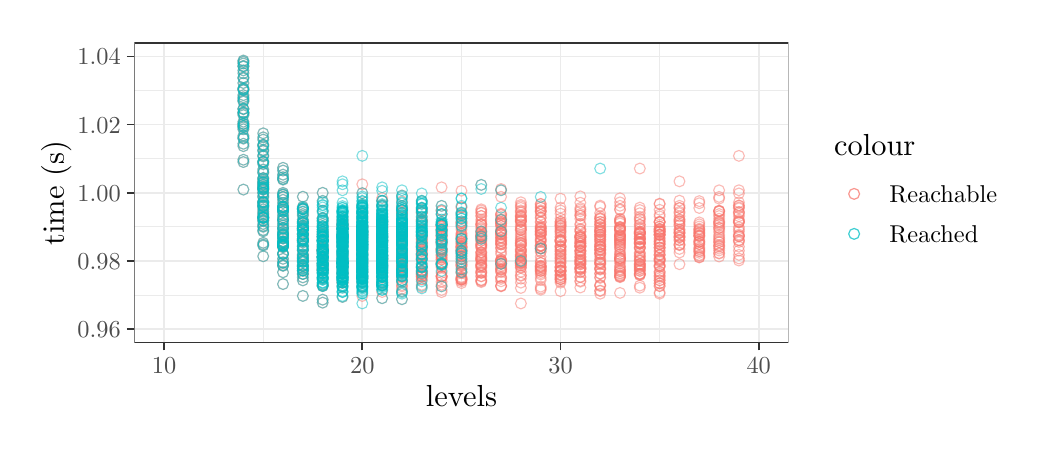
\begin{tikzpicture}[x=1pt,y=1pt]
\definecolor{fillColor}{RGB}{255,255,255}
\path[use as bounding box,fill=fillColor,fill opacity=0.00] (0,0) rectangle (361.35,144.54);
\begin{scope}
\path[clip] (  0.00,  0.00) rectangle (361.35,144.54);
\definecolor{drawColor}{RGB}{255,255,255}
\definecolor{fillColor}{RGB}{255,255,255}

\path[draw=drawColor,line width= 0.6pt,line join=round,line cap=round,fill=fillColor] (  0.00,  0.00) rectangle (361.35,144.54);
\end{scope}
\begin{scope}
\path[clip] ( 38.56, 30.69) rectangle (274.92,139.04);
\definecolor{fillColor}{RGB}{255,255,255}

\path[fill=fillColor] ( 38.56, 30.69) rectangle (274.92,139.04);
\definecolor{drawColor}{gray}{0.92}

\path[draw=drawColor,line width= 0.3pt,line join=round] ( 38.56, 47.92) --
	(274.92, 47.92);

\path[draw=drawColor,line width= 0.3pt,line join=round] ( 38.56, 72.55) --
	(274.92, 72.55);

\path[draw=drawColor,line width= 0.3pt,line join=round] ( 38.56, 97.18) --
	(274.92, 97.18);

\path[draw=drawColor,line width= 0.3pt,line join=round] ( 38.56,121.80) --
	(274.92,121.80);

\path[draw=drawColor,line width= 0.3pt,line join=round] ( 85.11, 30.69) --
	( 85.11,139.04);

\path[draw=drawColor,line width= 0.3pt,line join=round] (156.74, 30.69) --
	(156.74,139.04);

\path[draw=drawColor,line width= 0.3pt,line join=round] (228.36, 30.69) --
	(228.36,139.04);

\path[draw=drawColor,line width= 0.6pt,line join=round] ( 38.56, 35.61) --
	(274.92, 35.61);

\path[draw=drawColor,line width= 0.6pt,line join=round] ( 38.56, 60.24) --
	(274.92, 60.24);

\path[draw=drawColor,line width= 0.6pt,line join=round] ( 38.56, 84.86) --
	(274.92, 84.86);

\path[draw=drawColor,line width= 0.6pt,line join=round] ( 38.56,109.49) --
	(274.92,109.49);

\path[draw=drawColor,line width= 0.6pt,line join=round] ( 38.56,134.11) --
	(274.92,134.11);

\path[draw=drawColor,line width= 0.6pt,line join=round] ( 49.30, 30.69) --
	( 49.30,139.04);

\path[draw=drawColor,line width= 0.6pt,line join=round] (120.92, 30.69) --
	(120.92,139.04);

\path[draw=drawColor,line width= 0.6pt,line join=round] (192.55, 30.69) --
	(192.55,139.04);

\path[draw=drawColor,line width= 0.6pt,line join=round] (264.17, 30.69) --
	(264.17,139.04);
\definecolor{drawColor}{RGB}{248,118,109}

\path[draw=drawColor,draw opacity=0.50,line width= 0.4pt,line join=round,line cap=round] ( 77.95,113.96) circle (  1.96);

\path[draw=drawColor,draw opacity=0.50,line width= 0.4pt,line join=round,line cap=round] ( 77.95,130.49) circle (  1.96);

\path[draw=drawColor,draw opacity=0.50,line width= 0.4pt,line join=round,line cap=round] ( 77.95,109.85) circle (  1.96);

\path[draw=drawColor,draw opacity=0.50,line width= 0.4pt,line join=round,line cap=round] ( 77.95,122.17) circle (  1.96);

\path[draw=drawColor,draw opacity=0.50,line width= 0.4pt,line join=round,line cap=round] ( 77.95,119.40) circle (  1.96);

\path[draw=drawColor,draw opacity=0.50,line width= 0.4pt,line join=round,line cap=round] ( 77.95,126.59) circle (  1.96);

\path[draw=drawColor,draw opacity=0.50,line width= 0.4pt,line join=round,line cap=round] ( 77.95,105.45) circle (  1.96);

\path[draw=drawColor,draw opacity=0.50,line width= 0.4pt,line join=round,line cap=round] ( 77.95,107.83) circle (  1.96);

\path[draw=drawColor,draw opacity=0.50,line width= 0.4pt,line join=round,line cap=round] ( 77.95,132.19) circle (  1.96);

\path[draw=drawColor,draw opacity=0.50,line width= 0.4pt,line join=round,line cap=round] ( 77.95,112.94) circle (  1.96);

\path[draw=drawColor,draw opacity=0.50,line width= 0.4pt,line join=round,line cap=round] ( 77.95,108.52) circle (  1.96);

\path[draw=drawColor,draw opacity=0.50,line width= 0.4pt,line join=round,line cap=round] ( 77.95,120.16) circle (  1.96);

\path[draw=drawColor,draw opacity=0.50,line width= 0.4pt,line join=round,line cap=round] ( 77.95,108.95) circle (  1.96);

\path[draw=drawColor,draw opacity=0.50,line width= 0.4pt,line join=round,line cap=round] ( 77.95,132.66) circle (  1.96);

\path[draw=drawColor,draw opacity=0.50,line width= 0.4pt,line join=round,line cap=round] ( 85.11, 76.95) circle (  1.96);

\path[draw=drawColor,draw opacity=0.50,line width= 0.4pt,line join=round,line cap=round] ( 85.11, 75.87) circle (  1.96);

\path[draw=drawColor,draw opacity=0.50,line width= 0.4pt,line join=round,line cap=round] ( 85.11, 81.26) circle (  1.96);

\path[draw=drawColor,draw opacity=0.50,line width= 0.4pt,line join=round,line cap=round] ( 85.11, 83.75) circle (  1.96);

\path[draw=drawColor,draw opacity=0.50,line width= 0.4pt,line join=round,line cap=round] ( 85.11, 90.02) circle (  1.96);

\path[draw=drawColor,draw opacity=0.50,line width= 0.4pt,line join=round,line cap=round] ( 85.11, 86.97) circle (  1.96);

\path[draw=drawColor,draw opacity=0.50,line width= 0.4pt,line join=round,line cap=round] ( 85.11, 87.79) circle (  1.96);

\path[draw=drawColor,draw opacity=0.50,line width= 0.4pt,line join=round,line cap=round] ( 85.11,102.28) circle (  1.96);

\path[draw=drawColor,draw opacity=0.50,line width= 0.4pt,line join=round,line cap=round] ( 85.11, 86.31) circle (  1.96);

\path[draw=drawColor,draw opacity=0.50,line width= 0.4pt,line join=round,line cap=round] ( 85.11, 95.24) circle (  1.96);

\path[draw=drawColor,draw opacity=0.50,line width= 0.4pt,line join=round,line cap=round] ( 85.11, 87.21) circle (  1.96);

\path[draw=drawColor,draw opacity=0.50,line width= 0.4pt,line join=round,line cap=round] ( 85.11, 80.18) circle (  1.96);

\path[draw=drawColor,draw opacity=0.50,line width= 0.4pt,line join=round,line cap=round] ( 85.11, 87.77) circle (  1.96);

\path[draw=drawColor,draw opacity=0.50,line width= 0.4pt,line join=round,line cap=round] ( 85.11,104.90) circle (  1.96);

\path[draw=drawColor,draw opacity=0.50,line width= 0.4pt,line join=round,line cap=round] ( 85.11, 98.38) circle (  1.96);

\path[draw=drawColor,draw opacity=0.50,line width= 0.4pt,line join=round,line cap=round] ( 85.11, 88.61) circle (  1.96);

\path[draw=drawColor,draw opacity=0.50,line width= 0.4pt,line join=round,line cap=round] ( 85.11, 77.45) circle (  1.96);

\path[draw=drawColor,draw opacity=0.50,line width= 0.4pt,line join=round,line cap=round] ( 85.11,102.11) circle (  1.96);

\path[draw=drawColor,draw opacity=0.50,line width= 0.4pt,line join=round,line cap=round] ( 85.11,100.33) circle (  1.96);

\path[draw=drawColor,draw opacity=0.50,line width= 0.4pt,line join=round,line cap=round] ( 85.11, 88.82) circle (  1.96);

\path[draw=drawColor,draw opacity=0.50,line width= 0.4pt,line join=round,line cap=round] ( 85.11, 98.04) circle (  1.96);

\path[draw=drawColor,draw opacity=0.50,line width= 0.4pt,line join=round,line cap=round] ( 85.11, 93.29) circle (  1.96);

\path[draw=drawColor,draw opacity=0.50,line width= 0.4pt,line join=round,line cap=round] ( 85.11,104.09) circle (  1.96);

\path[draw=drawColor,draw opacity=0.50,line width= 0.4pt,line join=round,line cap=round] ( 85.11, 85.97) circle (  1.96);

\path[draw=drawColor,draw opacity=0.50,line width= 0.4pt,line join=round,line cap=round] ( 85.11, 92.05) circle (  1.96);

\path[draw=drawColor,draw opacity=0.50,line width= 0.4pt,line join=round,line cap=round] ( 85.11, 89.45) circle (  1.96);

\path[draw=drawColor,draw opacity=0.50,line width= 0.4pt,line join=round,line cap=round] ( 85.11, 86.15) circle (  1.96);

\path[draw=drawColor,draw opacity=0.50,line width= 0.4pt,line join=round,line cap=round] ( 85.11, 96.26) circle (  1.96);

\path[draw=drawColor,draw opacity=0.50,line width= 0.4pt,line join=round,line cap=round] ( 85.11, 90.23) circle (  1.96);

\path[draw=drawColor,draw opacity=0.50,line width= 0.4pt,line join=round,line cap=round] ( 85.11, 79.65) circle (  1.96);

\path[draw=drawColor,draw opacity=0.50,line width= 0.4pt,line join=round,line cap=round] ( 85.11, 95.88) circle (  1.96);

\path[draw=drawColor,draw opacity=0.50,line width= 0.4pt,line join=round,line cap=round] ( 85.11,101.69) circle (  1.96);

\path[draw=drawColor,draw opacity=0.50,line width= 0.4pt,line join=round,line cap=round] ( 85.11, 84.88) circle (  1.96);

\path[draw=drawColor,draw opacity=0.50,line width= 0.4pt,line join=round,line cap=round] ( 92.27, 70.41) circle (  1.96);

\path[draw=drawColor,draw opacity=0.50,line width= 0.4pt,line join=round,line cap=round] ( 92.27, 78.79) circle (  1.96);

\path[draw=drawColor,draw opacity=0.50,line width= 0.4pt,line join=round,line cap=round] ( 92.27, 78.53) circle (  1.96);

\path[draw=drawColor,draw opacity=0.50,line width= 0.4pt,line join=round,line cap=round] ( 92.27, 83.47) circle (  1.96);

\path[draw=drawColor,draw opacity=0.50,line width= 0.4pt,line join=round,line cap=round] ( 92.27, 68.42) circle (  1.96);

\path[draw=drawColor,draw opacity=0.50,line width= 0.4pt,line join=round,line cap=round] ( 92.27, 82.33) circle (  1.96);

\path[draw=drawColor,draw opacity=0.50,line width= 0.4pt,line join=round,line cap=round] ( 92.27, 93.89) circle (  1.96);

\path[draw=drawColor,draw opacity=0.50,line width= 0.4pt,line join=round,line cap=round] ( 92.27, 77.98) circle (  1.96);

\path[draw=drawColor,draw opacity=0.50,line width= 0.4pt,line join=round,line cap=round] ( 92.27, 75.15) circle (  1.96);

\path[draw=drawColor,draw opacity=0.50,line width= 0.4pt,line join=round,line cap=round] ( 92.27, 75.99) circle (  1.96);

\path[draw=drawColor,draw opacity=0.50,line width= 0.4pt,line join=round,line cap=round] ( 92.27, 79.91) circle (  1.96);

\path[draw=drawColor,draw opacity=0.50,line width= 0.4pt,line join=round,line cap=round] ( 92.27, 89.90) circle (  1.96);

\path[draw=drawColor,draw opacity=0.50,line width= 0.4pt,line join=round,line cap=round] ( 92.27, 78.94) circle (  1.96);

\path[draw=drawColor,draw opacity=0.50,line width= 0.4pt,line join=round,line cap=round] ( 92.27, 71.78) circle (  1.96);

\path[draw=drawColor,draw opacity=0.50,line width= 0.4pt,line join=round,line cap=round] ( 92.27, 79.42) circle (  1.96);

\path[draw=drawColor,draw opacity=0.50,line width= 0.4pt,line join=round,line cap=round] ( 92.27, 80.01) circle (  1.96);

\path[draw=drawColor,draw opacity=0.50,line width= 0.4pt,line join=round,line cap=round] ( 92.27, 79.59) circle (  1.96);

\path[draw=drawColor,draw opacity=0.50,line width= 0.4pt,line join=round,line cap=round] ( 92.27, 79.67) circle (  1.96);

\path[draw=drawColor,draw opacity=0.50,line width= 0.4pt,line join=round,line cap=round] ( 92.27, 84.84) circle (  1.96);

\path[draw=drawColor,draw opacity=0.50,line width= 0.4pt,line join=round,line cap=round] ( 92.27, 69.88) circle (  1.96);

\path[draw=drawColor,draw opacity=0.50,line width= 0.4pt,line join=round,line cap=round] ( 92.27, 84.31) circle (  1.96);

\path[draw=drawColor,draw opacity=0.50,line width= 0.4pt,line join=round,line cap=round] ( 92.27, 76.81) circle (  1.96);

\path[draw=drawColor,draw opacity=0.50,line width= 0.4pt,line join=round,line cap=round] ( 92.27, 78.09) circle (  1.96);

\path[draw=drawColor,draw opacity=0.50,line width= 0.4pt,line join=round,line cap=round] ( 92.27, 73.87) circle (  1.96);

\path[draw=drawColor,draw opacity=0.50,line width= 0.4pt,line join=round,line cap=round] ( 92.27, 90.51) circle (  1.96);

\path[draw=drawColor,draw opacity=0.50,line width= 0.4pt,line join=round,line cap=round] ( 92.27, 92.91) circle (  1.96);

\path[draw=drawColor,draw opacity=0.50,line width= 0.4pt,line join=round,line cap=round] ( 92.27, 69.60) circle (  1.96);

\path[draw=drawColor,draw opacity=0.50,line width= 0.4pt,line join=round,line cap=round] ( 92.27, 84.14) circle (  1.96);

\path[draw=drawColor,draw opacity=0.50,line width= 0.4pt,line join=round,line cap=round] ( 92.27, 66.41) circle (  1.96);

\path[draw=drawColor,draw opacity=0.50,line width= 0.4pt,line join=round,line cap=round] ( 92.27, 89.63) circle (  1.96);

\path[draw=drawColor,draw opacity=0.50,line width= 0.4pt,line join=round,line cap=round] ( 92.27, 91.42) circle (  1.96);

\path[draw=drawColor,draw opacity=0.50,line width= 0.4pt,line join=round,line cap=round] ( 92.27, 73.13) circle (  1.96);

\path[draw=drawColor,draw opacity=0.50,line width= 0.4pt,line join=round,line cap=round] ( 92.27, 75.17) circle (  1.96);

\path[draw=drawColor,draw opacity=0.50,line width= 0.4pt,line join=round,line cap=round] ( 99.44, 67.91) circle (  1.96);

\path[draw=drawColor,draw opacity=0.50,line width= 0.4pt,line join=round,line cap=round] ( 99.44, 79.03) circle (  1.96);

\path[draw=drawColor,draw opacity=0.50,line width= 0.4pt,line join=round,line cap=round] ( 99.44, 67.56) circle (  1.96);

\path[draw=drawColor,draw opacity=0.50,line width= 0.4pt,line join=round,line cap=round] ( 99.44, 70.07) circle (  1.96);

\path[draw=drawColor,draw opacity=0.50,line width= 0.4pt,line join=round,line cap=round] ( 99.44, 68.30) circle (  1.96);

\path[draw=drawColor,draw opacity=0.50,line width= 0.4pt,line join=round,line cap=round] ( 99.44, 72.05) circle (  1.96);

\path[draw=drawColor,draw opacity=0.50,line width= 0.4pt,line join=round,line cap=round] ( 99.44, 64.15) circle (  1.96);

\path[draw=drawColor,draw opacity=0.50,line width= 0.4pt,line join=round,line cap=round] ( 99.44, 74.09) circle (  1.96);

\path[draw=drawColor,draw opacity=0.50,line width= 0.4pt,line join=round,line cap=round] ( 99.44, 78.99) circle (  1.96);

\path[draw=drawColor,draw opacity=0.50,line width= 0.4pt,line join=round,line cap=round] ( 99.44, 72.94) circle (  1.96);

\path[draw=drawColor,draw opacity=0.50,line width= 0.4pt,line join=round,line cap=round] ( 99.44, 78.90) circle (  1.96);

\path[draw=drawColor,draw opacity=0.50,line width= 0.4pt,line join=round,line cap=round] ( 99.44, 74.48) circle (  1.96);

\path[draw=drawColor,draw opacity=0.50,line width= 0.4pt,line join=round,line cap=round] ( 99.44, 68.08) circle (  1.96);

\path[draw=drawColor,draw opacity=0.50,line width= 0.4pt,line join=round,line cap=round] ( 99.44, 75.22) circle (  1.96);

\path[draw=drawColor,draw opacity=0.50,line width= 0.4pt,line join=round,line cap=round] ( 99.44, 77.20) circle (  1.96);

\path[draw=drawColor,draw opacity=0.50,line width= 0.4pt,line join=round,line cap=round] ( 99.44, 77.95) circle (  1.96);

\path[draw=drawColor,draw opacity=0.50,line width= 0.4pt,line join=round,line cap=round] ( 99.44, 73.96) circle (  1.96);

\path[draw=drawColor,draw opacity=0.50,line width= 0.4pt,line join=round,line cap=round] ( 99.44, 79.32) circle (  1.96);

\path[draw=drawColor,draw opacity=0.50,line width= 0.4pt,line join=round,line cap=round] ( 99.44, 64.46) circle (  1.96);

\path[draw=drawColor,draw opacity=0.50,line width= 0.4pt,line join=round,line cap=round] ( 99.44, 66.92) circle (  1.96);

\path[draw=drawColor,draw opacity=0.50,line width= 0.4pt,line join=round,line cap=round] ( 99.44, 72.50) circle (  1.96);

\path[draw=drawColor,draw opacity=0.50,line width= 0.4pt,line join=round,line cap=round] ( 99.44, 69.88) circle (  1.96);

\path[draw=drawColor,draw opacity=0.50,line width= 0.4pt,line join=round,line cap=round] ( 99.44, 58.83) circle (  1.96);

\path[draw=drawColor,draw opacity=0.50,line width= 0.4pt,line join=round,line cap=round] ( 99.44, 71.97) circle (  1.96);

\path[draw=drawColor,draw opacity=0.50,line width= 0.4pt,line join=round,line cap=round] ( 99.44, 69.86) circle (  1.96);

\path[draw=drawColor,draw opacity=0.50,line width= 0.4pt,line join=round,line cap=round] ( 99.44, 69.12) circle (  1.96);

\path[draw=drawColor,draw opacity=0.50,line width= 0.4pt,line join=round,line cap=round] ( 99.44, 79.79) circle (  1.96);

\path[draw=drawColor,draw opacity=0.50,line width= 0.4pt,line join=round,line cap=round] ( 99.44, 71.37) circle (  1.96);

\path[draw=drawColor,draw opacity=0.50,line width= 0.4pt,line join=round,line cap=round] ( 99.44, 73.83) circle (  1.96);

\path[draw=drawColor,draw opacity=0.50,line width= 0.4pt,line join=round,line cap=round] ( 99.44, 72.00) circle (  1.96);

\path[draw=drawColor,draw opacity=0.50,line width= 0.4pt,line join=round,line cap=round] ( 99.44, 72.43) circle (  1.96);

\path[draw=drawColor,draw opacity=0.50,line width= 0.4pt,line join=round,line cap=round] ( 99.44, 61.97) circle (  1.96);

\path[draw=drawColor,draw opacity=0.50,line width= 0.4pt,line join=round,line cap=round] ( 99.44, 65.50) circle (  1.96);

\path[draw=drawColor,draw opacity=0.50,line width= 0.4pt,line join=round,line cap=round] (106.60, 84.86) circle (  1.96);

\path[draw=drawColor,draw opacity=0.50,line width= 0.4pt,line join=round,line cap=round] (106.60, 69.23) circle (  1.96);

\path[draw=drawColor,draw opacity=0.50,line width= 0.4pt,line join=round,line cap=round] (106.60, 67.50) circle (  1.96);

\path[draw=drawColor,draw opacity=0.50,line width= 0.4pt,line join=round,line cap=round] (106.60, 61.84) circle (  1.96);

\path[draw=drawColor,draw opacity=0.50,line width= 0.4pt,line join=round,line cap=round] (106.60, 67.71) circle (  1.96);

\path[draw=drawColor,draw opacity=0.50,line width= 0.4pt,line join=round,line cap=round] (106.60, 68.29) circle (  1.96);

\path[draw=drawColor,draw opacity=0.50,line width= 0.4pt,line join=round,line cap=round] (106.60, 74.70) circle (  1.96);

\path[draw=drawColor,draw opacity=0.50,line width= 0.4pt,line join=round,line cap=round] (106.60, 64.10) circle (  1.96);

\path[draw=drawColor,draw opacity=0.50,line width= 0.4pt,line join=round,line cap=round] (106.60, 67.83) circle (  1.96);

\path[draw=drawColor,draw opacity=0.50,line width= 0.4pt,line join=round,line cap=round] (106.60, 68.92) circle (  1.96);

\path[draw=drawColor,draw opacity=0.50,line width= 0.4pt,line join=round,line cap=round] (106.60, 64.83) circle (  1.96);

\path[draw=drawColor,draw opacity=0.50,line width= 0.4pt,line join=round,line cap=round] (106.60, 70.13) circle (  1.96);

\path[draw=drawColor,draw opacity=0.50,line width= 0.4pt,line join=round,line cap=round] (106.60, 69.85) circle (  1.96);

\path[draw=drawColor,draw opacity=0.50,line width= 0.4pt,line join=round,line cap=round] (106.60, 61.92) circle (  1.96);

\path[draw=drawColor,draw opacity=0.50,line width= 0.4pt,line join=round,line cap=round] (106.60, 57.52) circle (  1.96);

\path[draw=drawColor,draw opacity=0.50,line width= 0.4pt,line join=round,line cap=round] (106.60, 63.13) circle (  1.96);

\path[draw=drawColor,draw opacity=0.50,line width= 0.4pt,line join=round,line cap=round] (106.60, 63.43) circle (  1.96);

\path[draw=drawColor,draw opacity=0.50,line width= 0.4pt,line join=round,line cap=round] (106.60, 70.70) circle (  1.96);

\path[draw=drawColor,draw opacity=0.50,line width= 0.4pt,line join=round,line cap=round] (106.60, 68.92) circle (  1.96);

\path[draw=drawColor,draw opacity=0.50,line width= 0.4pt,line join=round,line cap=round] (106.60, 75.60) circle (  1.96);

\path[draw=drawColor,draw opacity=0.50,line width= 0.4pt,line join=round,line cap=round] (106.60, 61.30) circle (  1.96);

\path[draw=drawColor,draw opacity=0.50,line width= 0.4pt,line join=round,line cap=round] (106.60, 65.09) circle (  1.96);

\path[draw=drawColor,draw opacity=0.50,line width= 0.4pt,line join=round,line cap=round] (106.60, 75.78) circle (  1.96);

\path[draw=drawColor,draw opacity=0.50,line width= 0.4pt,line join=round,line cap=round] (106.60, 63.87) circle (  1.96);

\path[draw=drawColor,draw opacity=0.50,line width= 0.4pt,line join=round,line cap=round] (106.60, 73.62) circle (  1.96);

\path[draw=drawColor,draw opacity=0.50,line width= 0.4pt,line join=round,line cap=round] (106.60, 67.30) circle (  1.96);

\path[draw=drawColor,draw opacity=0.50,line width= 0.4pt,line join=round,line cap=round] (106.60, 65.39) circle (  1.96);

\path[draw=drawColor,draw opacity=0.50,line width= 0.4pt,line join=round,line cap=round] (106.60, 81.95) circle (  1.96);

\path[draw=drawColor,draw opacity=0.50,line width= 0.4pt,line join=round,line cap=round] (106.60, 63.78) circle (  1.96);

\path[draw=drawColor,draw opacity=0.50,line width= 0.4pt,line join=round,line cap=round] (106.60, 64.41) circle (  1.96);

\path[draw=drawColor,draw opacity=0.50,line width= 0.4pt,line join=round,line cap=round] (106.60, 62.75) circle (  1.96);

\path[draw=drawColor,draw opacity=0.50,line width= 0.4pt,line join=round,line cap=round] (106.60, 64.16) circle (  1.96);

\path[draw=drawColor,draw opacity=0.50,line width= 0.4pt,line join=round,line cap=round] (106.60, 69.00) circle (  1.96);

\path[draw=drawColor,draw opacity=0.50,line width= 0.4pt,line join=round,line cap=round] (113.76, 72.97) circle (  1.96);

\path[draw=drawColor,draw opacity=0.50,line width= 0.4pt,line join=round,line cap=round] (113.76, 73.76) circle (  1.96);

\path[draw=drawColor,draw opacity=0.50,line width= 0.4pt,line join=round,line cap=round] (113.76, 59.34) circle (  1.96);

\path[draw=drawColor,draw opacity=0.50,line width= 0.4pt,line join=round,line cap=round] (113.76, 70.00) circle (  1.96);

\path[draw=drawColor,draw opacity=0.50,line width= 0.4pt,line join=round,line cap=round] (113.76, 69.71) circle (  1.96);

\path[draw=drawColor,draw opacity=0.50,line width= 0.4pt,line join=round,line cap=round] (113.76, 69.31) circle (  1.96);

\path[draw=drawColor,draw opacity=0.50,line width= 0.4pt,line join=round,line cap=round] (113.76, 66.32) circle (  1.96);

\path[draw=drawColor,draw opacity=0.50,line width= 0.4pt,line join=round,line cap=round] (113.76, 58.16) circle (  1.96);

\path[draw=drawColor,draw opacity=0.50,line width= 0.4pt,line join=round,line cap=round] (113.76, 65.86) circle (  1.96);

\path[draw=drawColor,draw opacity=0.50,line width= 0.4pt,line join=round,line cap=round] (113.76, 66.92) circle (  1.96);

\path[draw=drawColor,draw opacity=0.50,line width= 0.4pt,line join=round,line cap=round] (113.76, 73.41) circle (  1.96);

\path[draw=drawColor,draw opacity=0.50,line width= 0.4pt,line join=round,line cap=round] (113.76, 73.18) circle (  1.96);

\path[draw=drawColor,draw opacity=0.50,line width= 0.4pt,line join=round,line cap=round] (113.76, 64.26) circle (  1.96);

\path[draw=drawColor,draw opacity=0.50,line width= 0.4pt,line join=round,line cap=round] (113.76, 73.17) circle (  1.96);

\path[draw=drawColor,draw opacity=0.50,line width= 0.4pt,line join=round,line cap=round] (113.76, 74.43) circle (  1.96);

\path[draw=drawColor,draw opacity=0.50,line width= 0.4pt,line join=round,line cap=round] (113.76, 63.01) circle (  1.96);

\path[draw=drawColor,draw opacity=0.50,line width= 0.4pt,line join=round,line cap=round] (113.76, 72.00) circle (  1.96);

\path[draw=drawColor,draw opacity=0.50,line width= 0.4pt,line join=round,line cap=round] (113.76, 74.87) circle (  1.96);

\path[draw=drawColor,draw opacity=0.50,line width= 0.4pt,line join=round,line cap=round] (113.76, 72.02) circle (  1.96);

\path[draw=drawColor,draw opacity=0.50,line width= 0.4pt,line join=round,line cap=round] (113.76, 73.81) circle (  1.96);

\path[draw=drawColor,draw opacity=0.50,line width= 0.4pt,line join=round,line cap=round] (113.76, 75.99) circle (  1.96);

\path[draw=drawColor,draw opacity=0.50,line width= 0.4pt,line join=round,line cap=round] (113.76, 69.82) circle (  1.96);

\path[draw=drawColor,draw opacity=0.50,line width= 0.4pt,line join=round,line cap=round] (113.76, 71.72) circle (  1.96);

\path[draw=drawColor,draw opacity=0.50,line width= 0.4pt,line join=round,line cap=round] (113.76, 69.07) circle (  1.96);

\path[draw=drawColor,draw opacity=0.50,line width= 0.4pt,line join=round,line cap=round] (113.76, 73.58) circle (  1.96);

\path[draw=drawColor,draw opacity=0.50,line width= 0.4pt,line join=round,line cap=round] (113.76, 72.53) circle (  1.96);

\path[draw=drawColor,draw opacity=0.50,line width= 0.4pt,line join=round,line cap=round] (113.76, 67.25) circle (  1.96);

\path[draw=drawColor,draw opacity=0.50,line width= 0.4pt,line join=round,line cap=round] (113.76, 61.97) circle (  1.96);

\path[draw=drawColor,draw opacity=0.50,line width= 0.4pt,line join=round,line cap=round] (113.76, 63.63) circle (  1.96);

\path[draw=drawColor,draw opacity=0.50,line width= 0.4pt,line join=round,line cap=round] (113.76, 71.67) circle (  1.96);

\path[draw=drawColor,draw opacity=0.50,line width= 0.4pt,line join=round,line cap=round] (113.76, 74.96) circle (  1.96);

\path[draw=drawColor,draw opacity=0.50,line width= 0.4pt,line join=round,line cap=round] (113.76, 62.17) circle (  1.96);

\path[draw=drawColor,draw opacity=0.50,line width= 0.4pt,line join=round,line cap=round] (113.76, 58.93) circle (  1.96);

\path[draw=drawColor,draw opacity=0.50,line width= 0.4pt,line join=round,line cap=round] (120.92, 64.10) circle (  1.96);

\path[draw=drawColor,draw opacity=0.50,line width= 0.4pt,line join=round,line cap=round] (120.92, 68.22) circle (  1.96);

\path[draw=drawColor,draw opacity=0.50,line width= 0.4pt,line join=round,line cap=round] (120.92, 78.12) circle (  1.96);

\path[draw=drawColor,draw opacity=0.50,line width= 0.4pt,line join=round,line cap=round] (120.92, 69.50) circle (  1.96);

\path[draw=drawColor,draw opacity=0.50,line width= 0.4pt,line join=round,line cap=round] (120.92, 72.93) circle (  1.96);

\path[draw=drawColor,draw opacity=0.50,line width= 0.4pt,line join=round,line cap=round] (120.92, 72.69) circle (  1.96);

\path[draw=drawColor,draw opacity=0.50,line width= 0.4pt,line join=round,line cap=round] (120.92, 63.97) circle (  1.96);

\path[draw=drawColor,draw opacity=0.50,line width= 0.4pt,line join=round,line cap=round] (120.92, 77.37) circle (  1.96);

\path[draw=drawColor,draw opacity=0.50,line width= 0.4pt,line join=round,line cap=round] (120.92, 72.46) circle (  1.96);

\path[draw=drawColor,draw opacity=0.50,line width= 0.4pt,line join=round,line cap=round] (120.92, 67.71) circle (  1.96);

\path[draw=drawColor,draw opacity=0.50,line width= 0.4pt,line join=round,line cap=round] (120.92, 64.58) circle (  1.96);

\path[draw=drawColor,draw opacity=0.50,line width= 0.4pt,line join=round,line cap=round] (120.92, 61.99) circle (  1.96);

\path[draw=drawColor,draw opacity=0.50,line width= 0.4pt,line join=round,line cap=round] (120.92, 75.33) circle (  1.96);

\path[draw=drawColor,draw opacity=0.50,line width= 0.4pt,line join=round,line cap=round] (120.92, 69.23) circle (  1.96);

\path[draw=drawColor,draw opacity=0.50,line width= 0.4pt,line join=round,line cap=round] (120.92, 77.45) circle (  1.96);

\path[draw=drawColor,draw opacity=0.50,line width= 0.4pt,line join=round,line cap=round] (120.92, 68.49) circle (  1.96);

\path[draw=drawColor,draw opacity=0.50,line width= 0.4pt,line join=round,line cap=round] (120.92, 72.40) circle (  1.96);

\path[draw=drawColor,draw opacity=0.50,line width= 0.4pt,line join=round,line cap=round] (120.92, 74.89) circle (  1.96);

\path[draw=drawColor,draw opacity=0.50,line width= 0.4pt,line join=round,line cap=round] (120.92, 59.88) circle (  1.96);

\path[draw=drawColor,draw opacity=0.50,line width= 0.4pt,line join=round,line cap=round] (120.92, 68.66) circle (  1.96);

\path[draw=drawColor,draw opacity=0.50,line width= 0.4pt,line join=round,line cap=round] (120.92, 69.75) circle (  1.96);

\path[draw=drawColor,draw opacity=0.50,line width= 0.4pt,line join=round,line cap=round] (120.92, 70.73) circle (  1.96);

\path[draw=drawColor,draw opacity=0.50,line width= 0.4pt,line join=round,line cap=round] (120.92, 71.02) circle (  1.96);

\path[draw=drawColor,draw opacity=0.50,line width= 0.4pt,line join=round,line cap=round] (120.92, 70.00) circle (  1.96);

\path[draw=drawColor,draw opacity=0.50,line width= 0.4pt,line join=round,line cap=round] (120.92, 84.74) circle (  1.96);

\path[draw=drawColor,draw opacity=0.50,line width= 0.4pt,line join=round,line cap=round] (120.92, 87.96) circle (  1.96);

\path[draw=drawColor,draw opacity=0.50,line width= 0.4pt,line join=round,line cap=round] (120.92, 80.52) circle (  1.96);

\path[draw=drawColor,draw opacity=0.50,line width= 0.4pt,line join=round,line cap=round] (120.92, 69.86) circle (  1.96);

\path[draw=drawColor,draw opacity=0.50,line width= 0.4pt,line join=round,line cap=round] (120.92, 70.85) circle (  1.96);

\path[draw=drawColor,draw opacity=0.50,line width= 0.4pt,line join=round,line cap=round] (120.92, 63.51) circle (  1.96);

\path[draw=drawColor,draw opacity=0.50,line width= 0.4pt,line join=round,line cap=round] (120.92, 72.55) circle (  1.96);

\path[draw=drawColor,draw opacity=0.50,line width= 0.4pt,line join=round,line cap=round] (120.92, 69.61) circle (  1.96);

\path[draw=drawColor,draw opacity=0.50,line width= 0.4pt,line join=round,line cap=round] (120.92, 68.57) circle (  1.96);

\path[draw=drawColor,draw opacity=0.50,line width= 0.4pt,line join=round,line cap=round] (128.09, 69.06) circle (  1.96);

\path[draw=drawColor,draw opacity=0.50,line width= 0.4pt,line join=round,line cap=round] (128.09, 78.39) circle (  1.96);

\path[draw=drawColor,draw opacity=0.50,line width= 0.4pt,line join=round,line cap=round] (128.09, 80.40) circle (  1.96);

\path[draw=drawColor,draw opacity=0.50,line width= 0.4pt,line join=round,line cap=round] (128.09, 67.59) circle (  1.96);

\path[draw=drawColor,draw opacity=0.50,line width= 0.4pt,line join=round,line cap=round] (128.09, 63.48) circle (  1.96);

\path[draw=drawColor,draw opacity=0.50,line width= 0.4pt,line join=round,line cap=round] (128.09, 70.26) circle (  1.96);

\path[draw=drawColor,draw opacity=0.50,line width= 0.4pt,line join=round,line cap=round] (128.09, 64.89) circle (  1.96);

\path[draw=drawColor,draw opacity=0.50,line width= 0.4pt,line join=round,line cap=round] (128.09, 61.75) circle (  1.96);

\path[draw=drawColor,draw opacity=0.50,line width= 0.4pt,line join=round,line cap=round] (128.09, 68.85) circle (  1.96);

\path[draw=drawColor,draw opacity=0.50,line width= 0.4pt,line join=round,line cap=round] (128.09, 81.97) circle (  1.96);

\path[draw=drawColor,draw opacity=0.50,line width= 0.4pt,line join=round,line cap=round] (128.09, 68.69) circle (  1.96);

\path[draw=drawColor,draw opacity=0.50,line width= 0.4pt,line join=round,line cap=round] (128.09, 81.95) circle (  1.96);

\path[draw=drawColor,draw opacity=0.50,line width= 0.4pt,line join=round,line cap=round] (128.09, 64.37) circle (  1.96);

\path[draw=drawColor,draw opacity=0.50,line width= 0.4pt,line join=round,line cap=round] (128.09, 72.50) circle (  1.96);

\path[draw=drawColor,draw opacity=0.50,line width= 0.4pt,line join=round,line cap=round] (128.09, 67.31) circle (  1.96);

\path[draw=drawColor,draw opacity=0.50,line width= 0.4pt,line join=round,line cap=round] (128.09, 73.01) circle (  1.96);

\path[draw=drawColor,draw opacity=0.50,line width= 0.4pt,line join=round,line cap=round] (128.09, 68.95) circle (  1.96);

\path[draw=drawColor,draw opacity=0.50,line width= 0.4pt,line join=round,line cap=round] (128.09, 66.82) circle (  1.96);

\path[draw=drawColor,draw opacity=0.50,line width= 0.4pt,line join=round,line cap=round] (128.09, 80.12) circle (  1.96);

\path[draw=drawColor,draw opacity=0.50,line width= 0.4pt,line join=round,line cap=round] (128.09, 73.98) circle (  1.96);

\path[draw=drawColor,draw opacity=0.50,line width= 0.4pt,line join=round,line cap=round] (128.09, 62.19) circle (  1.96);

\path[draw=drawColor,draw opacity=0.50,line width= 0.4pt,line join=round,line cap=round] (128.09, 72.37) circle (  1.96);

\path[draw=drawColor,draw opacity=0.50,line width= 0.4pt,line join=round,line cap=round] (128.09, 67.78) circle (  1.96);

\path[draw=drawColor,draw opacity=0.50,line width= 0.4pt,line join=round,line cap=round] (128.09, 73.56) circle (  1.96);

\path[draw=drawColor,draw opacity=0.50,line width= 0.4pt,line join=round,line cap=round] (128.09, 68.09) circle (  1.96);

\path[draw=drawColor,draw opacity=0.50,line width= 0.4pt,line join=round,line cap=round] (128.09, 69.95) circle (  1.96);

\path[draw=drawColor,draw opacity=0.50,line width= 0.4pt,line join=round,line cap=round] (128.09, 62.30) circle (  1.96);

\path[draw=drawColor,draw opacity=0.50,line width= 0.4pt,line join=round,line cap=round] (128.09, 82.98) circle (  1.96);

\path[draw=drawColor,draw opacity=0.50,line width= 0.4pt,line join=round,line cap=round] (128.09, 71.46) circle (  1.96);

\path[draw=drawColor,draw opacity=0.50,line width= 0.4pt,line join=round,line cap=round] (128.09, 72.14) circle (  1.96);

\path[draw=drawColor,draw opacity=0.50,line width= 0.4pt,line join=round,line cap=round] (128.09, 74.04) circle (  1.96);

\path[draw=drawColor,draw opacity=0.50,line width= 0.4pt,line join=round,line cap=round] (128.09, 73.12) circle (  1.96);

\path[draw=drawColor,draw opacity=0.50,line width= 0.4pt,line join=round,line cap=round] (128.09, 76.26) circle (  1.96);

\path[draw=drawColor,draw opacity=0.50,line width= 0.4pt,line join=round,line cap=round] (135.25, 77.78) circle (  1.96);

\path[draw=drawColor,draw opacity=0.50,line width= 0.4pt,line join=round,line cap=round] (135.25, 75.36) circle (  1.96);

\path[draw=drawColor,draw opacity=0.50,line width= 0.4pt,line join=round,line cap=round] (135.25, 70.66) circle (  1.96);

\path[draw=drawColor,draw opacity=0.50,line width= 0.4pt,line join=round,line cap=round] (135.25, 64.85) circle (  1.96);

\path[draw=drawColor,draw opacity=0.50,line width= 0.4pt,line join=round,line cap=round] (135.25, 69.24) circle (  1.96);

\path[draw=drawColor,draw opacity=0.50,line width= 0.4pt,line join=round,line cap=round] (135.25, 75.95) circle (  1.96);

\path[draw=drawColor,draw opacity=0.50,line width= 0.4pt,line join=round,line cap=round] (135.25, 78.76) circle (  1.96);

\path[draw=drawColor,draw opacity=0.50,line width= 0.4pt,line join=round,line cap=round] (135.25, 77.54) circle (  1.96);

\path[draw=drawColor,draw opacity=0.50,line width= 0.4pt,line join=round,line cap=round] (135.25, 58.90) circle (  1.96);

\path[draw=drawColor,draw opacity=0.50,line width= 0.4pt,line join=round,line cap=round] (135.25, 68.16) circle (  1.96);

\path[draw=drawColor,draw opacity=0.50,line width= 0.4pt,line join=round,line cap=round] (135.25, 78.51) circle (  1.96);

\path[draw=drawColor,draw opacity=0.50,line width= 0.4pt,line join=round,line cap=round] (135.25, 83.89) circle (  1.96);

\path[draw=drawColor,draw opacity=0.50,line width= 0.4pt,line join=round,line cap=round] (135.25, 62.98) circle (  1.96);

\path[draw=drawColor,draw opacity=0.50,line width= 0.4pt,line join=round,line cap=round] (135.25, 62.54) circle (  1.96);

\path[draw=drawColor,draw opacity=0.50,line width= 0.4pt,line join=round,line cap=round] (135.25, 67.19) circle (  1.96);

\path[draw=drawColor,draw opacity=0.50,line width= 0.4pt,line join=round,line cap=round] (135.25, 79.48) circle (  1.96);

\path[draw=drawColor,draw opacity=0.50,line width= 0.4pt,line join=round,line cap=round] (135.25, 71.87) circle (  1.96);

\path[draw=drawColor,draw opacity=0.50,line width= 0.4pt,line join=round,line cap=round] (135.25, 69.95) circle (  1.96);

\path[draw=drawColor,draw opacity=0.50,line width= 0.4pt,line join=round,line cap=round] (135.25, 72.50) circle (  1.96);

\path[draw=drawColor,draw opacity=0.50,line width= 0.4pt,line join=round,line cap=round] (135.25, 66.69) circle (  1.96);

\path[draw=drawColor,draw opacity=0.50,line width= 0.4pt,line join=round,line cap=round] (135.25, 69.07) circle (  1.96);

\path[draw=drawColor,draw opacity=0.50,line width= 0.4pt,line join=round,line cap=round] (135.25, 63.18) circle (  1.96);

\path[draw=drawColor,draw opacity=0.50,line width= 0.4pt,line join=round,line cap=round] (135.25, 71.24) circle (  1.96);

\path[draw=drawColor,draw opacity=0.50,line width= 0.4pt,line join=round,line cap=round] (135.25, 80.07) circle (  1.96);

\path[draw=drawColor,draw opacity=0.50,line width= 0.4pt,line join=round,line cap=round] (135.25, 70.17) circle (  1.96);

\path[draw=drawColor,draw opacity=0.50,line width= 0.4pt,line join=round,line cap=round] (135.25, 65.86) circle (  1.96);

\path[draw=drawColor,draw opacity=0.50,line width= 0.4pt,line join=round,line cap=round] (135.25, 70.89) circle (  1.96);

\path[draw=drawColor,draw opacity=0.50,line width= 0.4pt,line join=round,line cap=round] (135.25, 69.86) circle (  1.96);

\path[draw=drawColor,draw opacity=0.50,line width= 0.4pt,line join=round,line cap=round] (135.25, 68.60) circle (  1.96);

\path[draw=drawColor,draw opacity=0.50,line width= 0.4pt,line join=round,line cap=round] (135.25, 67.67) circle (  1.96);

\path[draw=drawColor,draw opacity=0.50,line width= 0.4pt,line join=round,line cap=round] (135.25, 77.65) circle (  1.96);

\path[draw=drawColor,draw opacity=0.50,line width= 0.4pt,line join=round,line cap=round] (135.25, 71.48) circle (  1.96);

\path[draw=drawColor,draw opacity=0.50,line width= 0.4pt,line join=round,line cap=round] (135.25, 66.56) circle (  1.96);

\path[draw=drawColor,draw opacity=0.50,line width= 0.4pt,line join=round,line cap=round] (142.41, 77.55) circle (  1.96);

\path[draw=drawColor,draw opacity=0.50,line width= 0.4pt,line join=round,line cap=round] (142.41, 73.24) circle (  1.96);

\path[draw=drawColor,draw opacity=0.50,line width= 0.4pt,line join=round,line cap=round] (142.41, 71.39) circle (  1.96);

\path[draw=drawColor,draw opacity=0.50,line width= 0.4pt,line join=round,line cap=round] (142.41, 74.98) circle (  1.96);

\path[draw=drawColor,draw opacity=0.50,line width= 0.4pt,line join=round,line cap=round] (142.41, 69.57) circle (  1.96);

\path[draw=drawColor,draw opacity=0.50,line width= 0.4pt,line join=round,line cap=round] (142.41, 73.86) circle (  1.96);

\path[draw=drawColor,draw opacity=0.50,line width= 0.4pt,line join=round,line cap=round] (142.41, 67.48) circle (  1.96);

\path[draw=drawColor,draw opacity=0.50,line width= 0.4pt,line join=round,line cap=round] (142.41, 69.10) circle (  1.96);

\path[draw=drawColor,draw opacity=0.50,line width= 0.4pt,line join=round,line cap=round] (142.41, 76.00) circle (  1.96);

\path[draw=drawColor,draw opacity=0.50,line width= 0.4pt,line join=round,line cap=round] (142.41, 62.26) circle (  1.96);

\path[draw=drawColor,draw opacity=0.50,line width= 0.4pt,line join=round,line cap=round] (142.41, 74.34) circle (  1.96);

\path[draw=drawColor,draw opacity=0.50,line width= 0.4pt,line join=round,line cap=round] (142.41, 79.41) circle (  1.96);

\path[draw=drawColor,draw opacity=0.50,line width= 0.4pt,line join=round,line cap=round] (142.41, 66.78) circle (  1.96);

\path[draw=drawColor,draw opacity=0.50,line width= 0.4pt,line join=round,line cap=round] (142.41, 75.14) circle (  1.96);

\path[draw=drawColor,draw opacity=0.50,line width= 0.4pt,line join=round,line cap=round] (142.41, 69.35) circle (  1.96);

\path[draw=drawColor,draw opacity=0.50,line width= 0.4pt,line join=round,line cap=round] (142.41, 67.27) circle (  1.96);

\path[draw=drawColor,draw opacity=0.50,line width= 0.4pt,line join=round,line cap=round] (142.41, 68.06) circle (  1.96);

\path[draw=drawColor,draw opacity=0.50,line width= 0.4pt,line join=round,line cap=round] (142.41, 70.61) circle (  1.96);

\path[draw=drawColor,draw opacity=0.50,line width= 0.4pt,line join=round,line cap=round] (142.41, 74.62) circle (  1.96);

\path[draw=drawColor,draw opacity=0.50,line width= 0.4pt,line join=round,line cap=round] (142.41, 81.94) circle (  1.96);

\path[draw=drawColor,draw opacity=0.50,line width= 0.4pt,line join=round,line cap=round] (142.41, 64.50) circle (  1.96);

\path[draw=drawColor,draw opacity=0.50,line width= 0.4pt,line join=round,line cap=round] (142.41, 65.35) circle (  1.96);

\path[draw=drawColor,draw opacity=0.50,line width= 0.4pt,line join=round,line cap=round] (142.41, 77.65) circle (  1.96);

\path[draw=drawColor,draw opacity=0.50,line width= 0.4pt,line join=round,line cap=round] (142.41, 66.90) circle (  1.96);

\path[draw=drawColor,draw opacity=0.50,line width= 0.4pt,line join=round,line cap=round] (142.41, 66.23) circle (  1.96);

\path[draw=drawColor,draw opacity=0.50,line width= 0.4pt,line join=round,line cap=round] (142.41, 69.14) circle (  1.96);

\path[draw=drawColor,draw opacity=0.50,line width= 0.4pt,line join=round,line cap=round] (142.41, 74.90) circle (  1.96);

\path[draw=drawColor,draw opacity=0.50,line width= 0.4pt,line join=round,line cap=round] (142.41, 62.79) circle (  1.96);

\path[draw=drawColor,draw opacity=0.50,line width= 0.4pt,line join=round,line cap=round] (142.41, 68.96) circle (  1.96);

\path[draw=drawColor,draw opacity=0.50,line width= 0.4pt,line join=round,line cap=round] (142.41, 67.98) circle (  1.96);

\path[draw=drawColor,draw opacity=0.50,line width= 0.4pt,line join=round,line cap=round] (142.41, 78.73) circle (  1.96);

\path[draw=drawColor,draw opacity=0.50,line width= 0.4pt,line join=round,line cap=round] (142.41, 65.54) circle (  1.96);

\path[draw=drawColor,draw opacity=0.50,line width= 0.4pt,line join=round,line cap=round] (142.41, 65.87) circle (  1.96);

\path[draw=drawColor,draw opacity=0.50,line width= 0.4pt,line join=round,line cap=round] (149.57, 69.70) circle (  1.96);

\path[draw=drawColor,draw opacity=0.50,line width= 0.4pt,line join=round,line cap=round] (149.57, 70.60) circle (  1.96);

\path[draw=drawColor,draw opacity=0.50,line width= 0.4pt,line join=round,line cap=round] (149.57, 78.47) circle (  1.96);

\path[draw=drawColor,draw opacity=0.50,line width= 0.4pt,line join=round,line cap=round] (149.57, 73.94) circle (  1.96);

\path[draw=drawColor,draw opacity=0.50,line width= 0.4pt,line join=round,line cap=round] (149.57, 76.99) circle (  1.96);

\path[draw=drawColor,draw opacity=0.50,line width= 0.4pt,line join=round,line cap=round] (149.57, 69.33) circle (  1.96);

\path[draw=drawColor,draw opacity=0.50,line width= 0.4pt,line join=round,line cap=round] (149.57, 66.99) circle (  1.96);

\path[draw=drawColor,draw opacity=0.50,line width= 0.4pt,line join=round,line cap=round] (149.57, 73.04) circle (  1.96);

\path[draw=drawColor,draw opacity=0.50,line width= 0.4pt,line join=round,line cap=round] (149.57, 58.28) circle (  1.96);

\path[draw=drawColor,draw opacity=0.50,line width= 0.4pt,line join=round,line cap=round] (149.57, 80.12) circle (  1.96);

\path[draw=drawColor,draw opacity=0.50,line width= 0.4pt,line join=round,line cap=round] (149.57, 71.00) circle (  1.96);

\path[draw=drawColor,draw opacity=0.50,line width= 0.4pt,line join=round,line cap=round] (149.57, 61.33) circle (  1.96);

\path[draw=drawColor,draw opacity=0.50,line width= 0.4pt,line join=round,line cap=round] (149.57, 67.13) circle (  1.96);

\path[draw=drawColor,draw opacity=0.50,line width= 0.4pt,line join=round,line cap=round] (149.57, 67.19) circle (  1.96);

\path[draw=drawColor,draw opacity=0.50,line width= 0.4pt,line join=round,line cap=round] (149.57, 71.78) circle (  1.96);

\path[draw=drawColor,draw opacity=0.50,line width= 0.4pt,line join=round,line cap=round] (149.57, 73.19) circle (  1.96);

\path[draw=drawColor,draw opacity=0.50,line width= 0.4pt,line join=round,line cap=round] (149.57, 71.31) circle (  1.96);

\path[draw=drawColor,draw opacity=0.50,line width= 0.4pt,line join=round,line cap=round] (149.57, 70.26) circle (  1.96);

\path[draw=drawColor,draw opacity=0.50,line width= 0.4pt,line join=round,line cap=round] (149.57, 72.06) circle (  1.96);

\path[draw=drawColor,draw opacity=0.50,line width= 0.4pt,line join=round,line cap=round] (149.57, 73.57) circle (  1.96);

\path[draw=drawColor,draw opacity=0.50,line width= 0.4pt,line join=round,line cap=round] (149.57, 73.19) circle (  1.96);

\path[draw=drawColor,draw opacity=0.50,line width= 0.4pt,line join=round,line cap=round] (149.57, 67.17) circle (  1.96);

\path[draw=drawColor,draw opacity=0.50,line width= 0.4pt,line join=round,line cap=round] (149.57, 69.15) circle (  1.96);

\path[draw=drawColor,draw opacity=0.50,line width= 0.4pt,line join=round,line cap=round] (149.57, 86.85) circle (  1.96);

\path[draw=drawColor,draw opacity=0.50,line width= 0.4pt,line join=round,line cap=round] (149.57, 71.06) circle (  1.96);

\path[draw=drawColor,draw opacity=0.50,line width= 0.4pt,line join=round,line cap=round] (149.57, 66.14) circle (  1.96);

\path[draw=drawColor,draw opacity=0.50,line width= 0.4pt,line join=round,line cap=round] (149.57, 72.69) circle (  1.96);

\path[draw=drawColor,draw opacity=0.50,line width= 0.4pt,line join=round,line cap=round] (149.57, 72.54) circle (  1.96);

\path[draw=drawColor,draw opacity=0.50,line width= 0.4pt,line join=round,line cap=round] (149.57, 64.28) circle (  1.96);

\path[draw=drawColor,draw opacity=0.50,line width= 0.4pt,line join=round,line cap=round] (149.57, 66.85) circle (  1.96);

\path[draw=drawColor,draw opacity=0.50,line width= 0.4pt,line join=round,line cap=round] (149.57, 64.67) circle (  1.96);

\path[draw=drawColor,draw opacity=0.50,line width= 0.4pt,line join=round,line cap=round] (149.57, 68.12) circle (  1.96);

\path[draw=drawColor,draw opacity=0.50,line width= 0.4pt,line join=round,line cap=round] (149.57, 68.72) circle (  1.96);

\path[draw=drawColor,draw opacity=0.50,line width= 0.4pt,line join=round,line cap=round] (156.74, 58.26) circle (  1.96);

\path[draw=drawColor,draw opacity=0.50,line width= 0.4pt,line join=round,line cap=round] (156.74, 73.73) circle (  1.96);

\path[draw=drawColor,draw opacity=0.50,line width= 0.4pt,line join=round,line cap=round] (156.74, 77.11) circle (  1.96);

\path[draw=drawColor,draw opacity=0.50,line width= 0.4pt,line join=round,line cap=round] (156.74, 72.26) circle (  1.96);

\path[draw=drawColor,draw opacity=0.50,line width= 0.4pt,line join=round,line cap=round] (156.74, 73.99) circle (  1.96);

\path[draw=drawColor,draw opacity=0.50,line width= 0.4pt,line join=round,line cap=round] (156.74, 62.00) circle (  1.96);

\path[draw=drawColor,draw opacity=0.50,line width= 0.4pt,line join=round,line cap=round] (156.74, 65.63) circle (  1.96);

\path[draw=drawColor,draw opacity=0.50,line width= 0.4pt,line join=round,line cap=round] (156.74, 71.55) circle (  1.96);

\path[draw=drawColor,draw opacity=0.50,line width= 0.4pt,line join=round,line cap=round] (156.74, 85.61) circle (  1.96);

\path[draw=drawColor,draw opacity=0.50,line width= 0.4pt,line join=round,line cap=round] (156.74, 67.25) circle (  1.96);

\path[draw=drawColor,draw opacity=0.50,line width= 0.4pt,line join=round,line cap=round] (156.74, 65.01) circle (  1.96);

\path[draw=drawColor,draw opacity=0.50,line width= 0.4pt,line join=round,line cap=round] (156.74, 67.23) circle (  1.96);

\path[draw=drawColor,draw opacity=0.50,line width= 0.4pt,line join=round,line cap=round] (156.74, 69.42) circle (  1.96);

\path[draw=drawColor,draw opacity=0.50,line width= 0.4pt,line join=round,line cap=round] (156.74, 64.32) circle (  1.96);

\path[draw=drawColor,draw opacity=0.50,line width= 0.4pt,line join=round,line cap=round] (156.74, 76.17) circle (  1.96);

\path[draw=drawColor,draw opacity=0.50,line width= 0.4pt,line join=round,line cap=round] (156.74, 69.99) circle (  1.96);

\path[draw=drawColor,draw opacity=0.50,line width= 0.4pt,line join=round,line cap=round] (156.74, 64.75) circle (  1.96);

\path[draw=drawColor,draw opacity=0.50,line width= 0.4pt,line join=round,line cap=round] (156.74, 68.58) circle (  1.96);

\path[draw=drawColor,draw opacity=0.50,line width= 0.4pt,line join=round,line cap=round] (156.74, 65.23) circle (  1.96);

\path[draw=drawColor,draw opacity=0.50,line width= 0.4pt,line join=round,line cap=round] (156.74, 68.94) circle (  1.96);

\path[draw=drawColor,draw opacity=0.50,line width= 0.4pt,line join=round,line cap=round] (156.74, 79.59) circle (  1.96);

\path[draw=drawColor,draw opacity=0.50,line width= 0.4pt,line join=round,line cap=round] (156.74, 63.30) circle (  1.96);

\path[draw=drawColor,draw opacity=0.50,line width= 0.4pt,line join=round,line cap=round] (156.74, 60.82) circle (  1.96);

\path[draw=drawColor,draw opacity=0.50,line width= 0.4pt,line join=round,line cap=round] (156.74, 74.36) circle (  1.96);

\path[draw=drawColor,draw opacity=0.50,line width= 0.4pt,line join=round,line cap=round] (156.74, 73.96) circle (  1.96);

\path[draw=drawColor,draw opacity=0.50,line width= 0.4pt,line join=round,line cap=round] (156.74, 59.87) circle (  1.96);

\path[draw=drawColor,draw opacity=0.50,line width= 0.4pt,line join=round,line cap=round] (156.74, 79.63) circle (  1.96);

\path[draw=drawColor,draw opacity=0.50,line width= 0.4pt,line join=round,line cap=round] (156.74, 65.71) circle (  1.96);

\path[draw=drawColor,draw opacity=0.50,line width= 0.4pt,line join=round,line cap=round] (156.74, 69.31) circle (  1.96);

\path[draw=drawColor,draw opacity=0.50,line width= 0.4pt,line join=round,line cap=round] (156.74, 64.11) circle (  1.96);

\path[draw=drawColor,draw opacity=0.50,line width= 0.4pt,line join=round,line cap=round] (156.74, 63.68) circle (  1.96);

\path[draw=drawColor,draw opacity=0.50,line width= 0.4pt,line join=round,line cap=round] (156.74, 66.29) circle (  1.96);

\path[draw=drawColor,draw opacity=0.50,line width= 0.4pt,line join=round,line cap=round] (156.74, 68.27) circle (  1.96);

\path[draw=drawColor,draw opacity=0.50,line width= 0.4pt,line join=round,line cap=round] (163.90, 67.50) circle (  1.96);

\path[draw=drawColor,draw opacity=0.50,line width= 0.4pt,line join=round,line cap=round] (163.90, 66.70) circle (  1.96);

\path[draw=drawColor,draw opacity=0.50,line width= 0.4pt,line join=round,line cap=round] (163.90, 75.22) circle (  1.96);

\path[draw=drawColor,draw opacity=0.50,line width= 0.4pt,line join=round,line cap=round] (163.90, 78.48) circle (  1.96);

\path[draw=drawColor,draw opacity=0.50,line width= 0.4pt,line join=round,line cap=round] (163.90, 63.35) circle (  1.96);

\path[draw=drawColor,draw opacity=0.50,line width= 0.4pt,line join=round,line cap=round] (163.90, 70.29) circle (  1.96);

\path[draw=drawColor,draw opacity=0.50,line width= 0.4pt,line join=round,line cap=round] (163.90, 69.39) circle (  1.96);

\path[draw=drawColor,draw opacity=0.50,line width= 0.4pt,line join=round,line cap=round] (163.90, 69.25) circle (  1.96);

\path[draw=drawColor,draw opacity=0.50,line width= 0.4pt,line join=round,line cap=round] (163.90, 73.48) circle (  1.96);

\path[draw=drawColor,draw opacity=0.50,line width= 0.4pt,line join=round,line cap=round] (163.90, 61.62) circle (  1.96);

\path[draw=drawColor,draw opacity=0.50,line width= 0.4pt,line join=round,line cap=round] (163.90, 62.13) circle (  1.96);

\path[draw=drawColor,draw opacity=0.50,line width= 0.4pt,line join=round,line cap=round] (163.90, 72.43) circle (  1.96);

\path[draw=drawColor,draw opacity=0.50,line width= 0.4pt,line join=round,line cap=round] (163.90, 87.73) circle (  1.96);

\path[draw=drawColor,draw opacity=0.50,line width= 0.4pt,line join=round,line cap=round] (163.90, 64.91) circle (  1.96);

\path[draw=drawColor,draw opacity=0.50,line width= 0.4pt,line join=round,line cap=round] (163.90, 68.38) circle (  1.96);

\path[draw=drawColor,draw opacity=0.50,line width= 0.4pt,line join=round,line cap=round] (163.90, 73.36) circle (  1.96);

\path[draw=drawColor,draw opacity=0.50,line width= 0.4pt,line join=round,line cap=round] (163.90, 70.98) circle (  1.96);

\path[draw=drawColor,draw opacity=0.50,line width= 0.4pt,line join=round,line cap=round] (163.90, 69.00) circle (  1.96);

\path[draw=drawColor,draw opacity=0.50,line width= 0.4pt,line join=round,line cap=round] (163.90, 66.20) circle (  1.96);

\path[draw=drawColor,draw opacity=0.50,line width= 0.4pt,line join=round,line cap=round] (163.90, 68.73) circle (  1.96);

\path[draw=drawColor,draw opacity=0.50,line width= 0.4pt,line join=round,line cap=round] (163.90, 69.09) circle (  1.96);

\path[draw=drawColor,draw opacity=0.50,line width= 0.4pt,line join=round,line cap=round] (163.90, 70.64) circle (  1.96);

\path[draw=drawColor,draw opacity=0.50,line width= 0.4pt,line join=round,line cap=round] (163.90, 74.48) circle (  1.96);

\path[draw=drawColor,draw opacity=0.50,line width= 0.4pt,line join=round,line cap=round] (163.90, 77.57) circle (  1.96);

\path[draw=drawColor,draw opacity=0.50,line width= 0.4pt,line join=round,line cap=round] (163.90, 67.58) circle (  1.96);

\path[draw=drawColor,draw opacity=0.50,line width= 0.4pt,line join=round,line cap=round] (163.90, 60.94) circle (  1.96);

\path[draw=drawColor,draw opacity=0.50,line width= 0.4pt,line join=round,line cap=round] (163.90, 62.54) circle (  1.96);

\path[draw=drawColor,draw opacity=0.50,line width= 0.4pt,line join=round,line cap=round] (163.90, 71.91) circle (  1.96);

\path[draw=drawColor,draw opacity=0.50,line width= 0.4pt,line join=round,line cap=round] (163.90, 60.30) circle (  1.96);

\path[draw=drawColor,draw opacity=0.50,line width= 0.4pt,line join=round,line cap=round] (163.90, 77.80) circle (  1.96);

\path[draw=drawColor,draw opacity=0.50,line width= 0.4pt,line join=round,line cap=round] (163.90, 73.20) circle (  1.96);

\path[draw=drawColor,draw opacity=0.50,line width= 0.4pt,line join=round,line cap=round] (163.90, 76.46) circle (  1.96);

\path[draw=drawColor,draw opacity=0.50,line width= 0.4pt,line join=round,line cap=round] (163.90, 69.71) circle (  1.96);

\path[draw=drawColor,draw opacity=0.50,line width= 0.4pt,line join=round,line cap=round] (171.06, 70.55) circle (  1.96);

\path[draw=drawColor,draw opacity=0.50,line width= 0.4pt,line join=round,line cap=round] (171.06, 77.08) circle (  1.96);

\path[draw=drawColor,draw opacity=0.50,line width= 0.4pt,line join=round,line cap=round] (171.06, 69.67) circle (  1.96);

\path[draw=drawColor,draw opacity=0.50,line width= 0.4pt,line join=round,line cap=round] (171.06, 70.17) circle (  1.96);

\path[draw=drawColor,draw opacity=0.50,line width= 0.4pt,line join=round,line cap=round] (171.06, 66.23) circle (  1.96);

\path[draw=drawColor,draw opacity=0.50,line width= 0.4pt,line join=round,line cap=round] (171.06, 67.48) circle (  1.96);

\path[draw=drawColor,draw opacity=0.50,line width= 0.4pt,line join=round,line cap=round] (171.06, 73.04) circle (  1.96);

\path[draw=drawColor,draw opacity=0.50,line width= 0.4pt,line join=round,line cap=round] (171.06, 75.44) circle (  1.96);

\path[draw=drawColor,draw opacity=0.50,line width= 0.4pt,line join=round,line cap=round] (171.06, 73.98) circle (  1.96);

\path[draw=drawColor,draw opacity=0.50,line width= 0.4pt,line join=round,line cap=round] (171.06, 73.93) circle (  1.96);

\path[draw=drawColor,draw opacity=0.50,line width= 0.4pt,line join=round,line cap=round] (171.06, 75.09) circle (  1.96);

\path[draw=drawColor,draw opacity=0.50,line width= 0.4pt,line join=round,line cap=round] (171.06, 75.09) circle (  1.96);

\path[draw=drawColor,draw opacity=0.50,line width= 0.4pt,line join=round,line cap=round] (171.06, 66.76) circle (  1.96);

\path[draw=drawColor,draw opacity=0.50,line width= 0.4pt,line join=round,line cap=round] (171.06, 68.83) circle (  1.96);

\path[draw=drawColor,draw opacity=0.50,line width= 0.4pt,line join=round,line cap=round] (171.06, 74.43) circle (  1.96);

\path[draw=drawColor,draw opacity=0.50,line width= 0.4pt,line join=round,line cap=round] (171.06, 60.23) circle (  1.96);

\path[draw=drawColor,draw opacity=0.50,line width= 0.4pt,line join=round,line cap=round] (171.06, 86.25) circle (  1.96);

\path[draw=drawColor,draw opacity=0.50,line width= 0.4pt,line join=round,line cap=round] (171.06, 85.79) circle (  1.96);

\path[draw=drawColor,draw opacity=0.50,line width= 0.4pt,line join=round,line cap=round] (171.06, 65.03) circle (  1.96);

\path[draw=drawColor,draw opacity=0.50,line width= 0.4pt,line join=round,line cap=round] (171.06, 76.12) circle (  1.96);

\path[draw=drawColor,draw opacity=0.50,line width= 0.4pt,line join=round,line cap=round] (171.06, 70.89) circle (  1.96);

\path[draw=drawColor,draw opacity=0.50,line width= 0.4pt,line join=round,line cap=round] (171.06, 70.80) circle (  1.96);

\path[draw=drawColor,draw opacity=0.50,line width= 0.4pt,line join=round,line cap=round] (171.06, 74.48) circle (  1.96);

\path[draw=drawColor,draw opacity=0.50,line width= 0.4pt,line join=round,line cap=round] (171.06, 83.43) circle (  1.96);

\path[draw=drawColor,draw opacity=0.50,line width= 0.4pt,line join=round,line cap=round] (171.06, 64.85) circle (  1.96);

\path[draw=drawColor,draw opacity=0.50,line width= 0.4pt,line join=round,line cap=round] (171.06, 67.81) circle (  1.96);

\path[draw=drawColor,draw opacity=0.50,line width= 0.4pt,line join=round,line cap=round] (171.06, 60.13) circle (  1.96);

\path[draw=drawColor,draw opacity=0.50,line width= 0.4pt,line join=round,line cap=round] (171.06, 73.70) circle (  1.96);

\path[draw=drawColor,draw opacity=0.50,line width= 0.4pt,line join=round,line cap=round] (171.06, 59.90) circle (  1.96);

\path[draw=drawColor,draw opacity=0.50,line width= 0.4pt,line join=round,line cap=round] (171.06, 71.22) circle (  1.96);

\path[draw=drawColor,draw opacity=0.50,line width= 0.4pt,line join=round,line cap=round] (171.06, 71.70) circle (  1.96);

\path[draw=drawColor,draw opacity=0.50,line width= 0.4pt,line join=round,line cap=round] (171.06, 76.83) circle (  1.96);

\path[draw=drawColor,draw opacity=0.50,line width= 0.4pt,line join=round,line cap=round] (171.06, 77.34) circle (  1.96);

\path[draw=drawColor,draw opacity=0.50,line width= 0.4pt,line join=round,line cap=round] (178.22, 74.93) circle (  1.96);

\path[draw=drawColor,draw opacity=0.50,line width= 0.4pt,line join=round,line cap=round] (178.22, 80.52) circle (  1.96);

\path[draw=drawColor,draw opacity=0.50,line width= 0.4pt,line join=round,line cap=round] (178.22, 59.61) circle (  1.96);

\path[draw=drawColor,draw opacity=0.50,line width= 0.4pt,line join=round,line cap=round] (178.22, 68.21) circle (  1.96);

\path[draw=drawColor,draw opacity=0.50,line width= 0.4pt,line join=round,line cap=round] (178.22, 74.63) circle (  1.96);

\path[draw=drawColor,draw opacity=0.50,line width= 0.4pt,line join=round,line cap=round] (178.22, 73.32) circle (  1.96);

\path[draw=drawColor,draw opacity=0.50,line width= 0.4pt,line join=round,line cap=round] (178.22, 77.74) circle (  1.96);

\path[draw=drawColor,draw opacity=0.50,line width= 0.4pt,line join=round,line cap=round] (178.22, 71.72) circle (  1.96);

\path[draw=drawColor,draw opacity=0.50,line width= 0.4pt,line join=round,line cap=round] (178.22, 67.43) circle (  1.96);

\path[draw=drawColor,draw opacity=0.50,line width= 0.4pt,line join=round,line cap=round] (178.22, 76.51) circle (  1.96);

\path[draw=drawColor,draw opacity=0.50,line width= 0.4pt,line join=round,line cap=round] (178.22, 80.01) circle (  1.96);

\path[draw=drawColor,draw opacity=0.50,line width= 0.4pt,line join=round,line cap=round] (178.22, 72.58) circle (  1.96);

\path[draw=drawColor,draw opacity=0.50,line width= 0.4pt,line join=round,line cap=round] (178.22, 76.76) circle (  1.96);

\path[draw=drawColor,draw opacity=0.50,line width= 0.4pt,line join=round,line cap=round] (178.22, 69.60) circle (  1.96);

\path[draw=drawColor,draw opacity=0.50,line width= 0.4pt,line join=round,line cap=round] (178.22, 75.63) circle (  1.96);

\path[draw=drawColor,draw opacity=0.50,line width= 0.4pt,line join=round,line cap=round] (178.22, 66.69) circle (  1.96);

\path[draw=drawColor,draw opacity=0.50,line width= 0.4pt,line join=round,line cap=round] (178.22, 72.27) circle (  1.96);

\path[draw=drawColor,draw opacity=0.50,line width= 0.4pt,line join=round,line cap=round] (178.22, 74.54) circle (  1.96);

\path[draw=drawColor,draw opacity=0.50,line width= 0.4pt,line join=round,line cap=round] (178.22, 63.43) circle (  1.96);

\path[draw=drawColor,draw opacity=0.50,line width= 0.4pt,line join=round,line cap=round] (178.22, 79.44) circle (  1.96);

\path[draw=drawColor,draw opacity=0.50,line width= 0.4pt,line join=round,line cap=round] (178.22, 65.67) circle (  1.96);

\path[draw=drawColor,draw opacity=0.50,line width= 0.4pt,line join=round,line cap=round] (178.22, 78.50) circle (  1.96);

\path[draw=drawColor,draw opacity=0.50,line width= 0.4pt,line join=round,line cap=round] (178.22, 70.39) circle (  1.96);

\path[draw=drawColor,draw opacity=0.50,line width= 0.4pt,line join=round,line cap=round] (178.22, 66.76) circle (  1.96);

\path[draw=drawColor,draw opacity=0.50,line width= 0.4pt,line join=round,line cap=round] (178.22, 64.37) circle (  1.96);

\path[draw=drawColor,draw opacity=0.50,line width= 0.4pt,line join=round,line cap=round] (178.22, 76.09) circle (  1.96);

\path[draw=drawColor,draw opacity=0.50,line width= 0.4pt,line join=round,line cap=round] (178.22, 78.09) circle (  1.96);

\path[draw=drawColor,draw opacity=0.50,line width= 0.4pt,line join=round,line cap=round] (178.22, 76.35) circle (  1.96);

\path[draw=drawColor,draw opacity=0.50,line width= 0.4pt,line join=round,line cap=round] (178.22, 71.44) circle (  1.96);

\path[draw=drawColor,draw opacity=0.50,line width= 0.4pt,line join=round,line cap=round] (178.22, 81.46) circle (  1.96);

\path[draw=drawColor,draw opacity=0.50,line width= 0.4pt,line join=round,line cap=round] (178.22, 62.56) circle (  1.96);

\path[draw=drawColor,draw opacity=0.50,line width= 0.4pt,line join=round,line cap=round] (178.22, 74.36) circle (  1.96);

\path[draw=drawColor,draw opacity=0.50,line width= 0.4pt,line join=round,line cap=round] (178.22, 75.14) circle (  1.96);

\path[draw=drawColor,draw opacity=0.50,line width= 0.4pt,line join=round,line cap=round] (185.39, 74.26) circle (  1.96);

\path[draw=drawColor,draw opacity=0.50,line width= 0.4pt,line join=round,line cap=round] (185.39, 69.84) circle (  1.96);

\path[draw=drawColor,draw opacity=0.50,line width= 0.4pt,line join=round,line cap=round] (185.39, 79.49) circle (  1.96);

\path[draw=drawColor,draw opacity=0.50,line width= 0.4pt,line join=round,line cap=round] (185.39, 70.71) circle (  1.96);

\path[draw=drawColor,draw opacity=0.50,line width= 0.4pt,line join=round,line cap=round] (185.39, 78.58) circle (  1.96);

\path[draw=drawColor,draw opacity=0.50,line width= 0.4pt,line join=round,line cap=round] (185.39, 75.79) circle (  1.96);

\path[draw=drawColor,draw opacity=0.50,line width= 0.4pt,line join=round,line cap=round] (185.39, 74.34) circle (  1.96);

\path[draw=drawColor,draw opacity=0.50,line width= 0.4pt,line join=round,line cap=round] (185.39, 63.84) circle (  1.96);

\path[draw=drawColor,draw opacity=0.50,line width= 0.4pt,line join=round,line cap=round] (185.39, 78.21) circle (  1.96);

\path[draw=drawColor,draw opacity=0.50,line width= 0.4pt,line join=round,line cap=round] (185.39, 63.48) circle (  1.96);

\path[draw=drawColor,draw opacity=0.50,line width= 0.4pt,line join=round,line cap=round] (185.39, 75.91) circle (  1.96);

\path[draw=drawColor,draw opacity=0.50,line width= 0.4pt,line join=round,line cap=round] (185.39, 77.99) circle (  1.96);

\path[draw=drawColor,draw opacity=0.50,line width= 0.4pt,line join=round,line cap=round] (185.39, 67.07) circle (  1.96);

\path[draw=drawColor,draw opacity=0.50,line width= 0.4pt,line join=round,line cap=round] (185.39, 72.58) circle (  1.96);

\path[draw=drawColor,draw opacity=0.50,line width= 0.4pt,line join=round,line cap=round] (185.39, 67.48) circle (  1.96);

\path[draw=drawColor,draw opacity=0.50,line width= 0.4pt,line join=round,line cap=round] (185.39, 72.90) circle (  1.96);

\path[draw=drawColor,draw opacity=0.50,line width= 0.4pt,line join=round,line cap=round] (185.39, 78.15) circle (  1.96);

\path[draw=drawColor,draw opacity=0.50,line width= 0.4pt,line join=round,line cap=round] (185.39, 65.88) circle (  1.96);

\path[draw=drawColor,draw opacity=0.50,line width= 0.4pt,line join=round,line cap=round] (185.39, 70.90) circle (  1.96);

\path[draw=drawColor,draw opacity=0.50,line width= 0.4pt,line join=round,line cap=round] (185.39, 67.91) circle (  1.96);

\path[draw=drawColor,draw opacity=0.50,line width= 0.4pt,line join=round,line cap=round] (185.39, 80.09) circle (  1.96);

\path[draw=drawColor,draw opacity=0.50,line width= 0.4pt,line join=round,line cap=round] (185.39, 68.56) circle (  1.96);

\path[draw=drawColor,draw opacity=0.50,line width= 0.4pt,line join=round,line cap=round] (185.39, 64.83) circle (  1.96);

\path[draw=drawColor,draw opacity=0.50,line width= 0.4pt,line join=round,line cap=round] (185.39, 80.88) circle (  1.96);

\path[draw=drawColor,draw opacity=0.50,line width= 0.4pt,line join=round,line cap=round] (185.39, 70.50) circle (  1.96);

\path[draw=drawColor,draw opacity=0.50,line width= 0.4pt,line join=round,line cap=round] (185.39, 65.52) circle (  1.96);

\path[draw=drawColor,draw opacity=0.50,line width= 0.4pt,line join=round,line cap=round] (185.39, 69.67) circle (  1.96);

\path[draw=drawColor,draw opacity=0.50,line width= 0.4pt,line join=round,line cap=round] (185.39, 72.02) circle (  1.96);

\path[draw=drawColor,draw opacity=0.50,line width= 0.4pt,line join=round,line cap=round] (185.39, 65.72) circle (  1.96);

\path[draw=drawColor,draw opacity=0.50,line width= 0.4pt,line join=round,line cap=round] (185.39, 71.15) circle (  1.96);

\path[draw=drawColor,draw opacity=0.50,line width= 0.4pt,line join=round,line cap=round] (185.39, 72.04) circle (  1.96);

\path[draw=drawColor,draw opacity=0.50,line width= 0.4pt,line join=round,line cap=round] (185.39, 80.80) circle (  1.96);

\path[draw=drawColor,draw opacity=0.50,line width= 0.4pt,line join=round,line cap=round] (185.39, 76.90) circle (  1.96);

\path[draw=drawColor,draw opacity=0.50,line width= 0.4pt,line join=round,line cap=round] (192.55, 69.88) circle (  1.96);

\path[draw=drawColor,draw opacity=0.50,line width= 0.4pt,line join=round,line cap=round] (192.55, 67.64) circle (  1.96);

\path[draw=drawColor,draw opacity=0.50,line width= 0.4pt,line join=round,line cap=round] (192.55, 67.23) circle (  1.96);

\path[draw=drawColor,draw opacity=0.50,line width= 0.4pt,line join=round,line cap=round] (192.55, 72.83) circle (  1.96);

\path[draw=drawColor,draw opacity=0.50,line width= 0.4pt,line join=round,line cap=round] (192.55, 61.69) circle (  1.96);

\path[draw=drawColor,draw opacity=0.50,line width= 0.4pt,line join=round,line cap=round] (192.55, 67.28) circle (  1.96);

\path[draw=drawColor,draw opacity=0.50,line width= 0.4pt,line join=round,line cap=round] (192.55, 63.70) circle (  1.96);

\path[draw=drawColor,draw opacity=0.50,line width= 0.4pt,line join=round,line cap=round] (192.55, 74.40) circle (  1.96);

\path[draw=drawColor,draw opacity=0.50,line width= 0.4pt,line join=round,line cap=round] (192.55, 73.12) circle (  1.96);

\path[draw=drawColor,draw opacity=0.50,line width= 0.4pt,line join=round,line cap=round] (192.55, 70.65) circle (  1.96);

\path[draw=drawColor,draw opacity=0.50,line width= 0.4pt,line join=round,line cap=round] (192.55, 82.75) circle (  1.96);

\path[draw=drawColor,draw opacity=0.50,line width= 0.4pt,line join=round,line cap=round] (192.55, 63.64) circle (  1.96);

\path[draw=drawColor,draw opacity=0.50,line width= 0.4pt,line join=round,line cap=round] (192.55, 77.33) circle (  1.96);

\path[draw=drawColor,draw opacity=0.50,line width= 0.4pt,line join=round,line cap=round] (192.55, 75.56) circle (  1.96);

\path[draw=drawColor,draw opacity=0.50,line width= 0.4pt,line join=round,line cap=round] (192.55, 78.49) circle (  1.96);

\path[draw=drawColor,draw opacity=0.50,line width= 0.4pt,line join=round,line cap=round] (192.55, 64.19) circle (  1.96);

\path[draw=drawColor,draw opacity=0.50,line width= 0.4pt,line join=round,line cap=round] (192.55, 62.69) circle (  1.96);

\path[draw=drawColor,draw opacity=0.50,line width= 0.4pt,line join=round,line cap=round] (192.55, 59.62) circle (  1.96);

\path[draw=drawColor,draw opacity=0.50,line width= 0.4pt,line join=round,line cap=round] (192.55, 67.81) circle (  1.96);

\path[draw=drawColor,draw opacity=0.50,line width= 0.4pt,line join=round,line cap=round] (192.55, 71.30) circle (  1.96);

\path[draw=drawColor,draw opacity=0.50,line width= 0.4pt,line join=round,line cap=round] (192.55, 67.90) circle (  1.96);

\path[draw=drawColor,draw opacity=0.50,line width= 0.4pt,line join=round,line cap=round] (192.55, 74.45) circle (  1.96);

\path[draw=drawColor,draw opacity=0.50,line width= 0.4pt,line join=round,line cap=round] (192.55, 64.55) circle (  1.96);

\path[draw=drawColor,draw opacity=0.50,line width= 0.4pt,line join=round,line cap=round] (192.55, 67.77) circle (  1.96);

\path[draw=drawColor,draw opacity=0.50,line width= 0.4pt,line join=round,line cap=round] (192.55, 70.89) circle (  1.96);

\path[draw=drawColor,draw opacity=0.50,line width= 0.4pt,line join=round,line cap=round] (192.55, 79.51) circle (  1.96);

\path[draw=drawColor,draw opacity=0.50,line width= 0.4pt,line join=round,line cap=round] (192.55, 56.26) circle (  1.96);

\path[draw=drawColor,draw opacity=0.50,line width= 0.4pt,line join=round,line cap=round] (192.55, 72.30) circle (  1.96);

\path[draw=drawColor,draw opacity=0.50,line width= 0.4pt,line join=round,line cap=round] (192.55, 68.83) circle (  1.96);

\path[draw=drawColor,draw opacity=0.50,line width= 0.4pt,line join=round,line cap=round] (192.55, 71.88) circle (  1.96);

\path[draw=drawColor,draw opacity=0.50,line width= 0.4pt,line join=round,line cap=round] (192.55, 73.53) circle (  1.96);

\path[draw=drawColor,draw opacity=0.50,line width= 0.4pt,line join=round,line cap=round] (192.55, 67.29) circle (  1.96);

\path[draw=drawColor,draw opacity=0.50,line width= 0.4pt,line join=round,line cap=round] (192.55, 65.29) circle (  1.96);

\path[draw=drawColor,draw opacity=0.50,line width= 0.4pt,line join=round,line cap=round] (199.71, 67.12) circle (  1.96);

\path[draw=drawColor,draw opacity=0.50,line width= 0.4pt,line join=round,line cap=round] (199.71, 73.64) circle (  1.96);

\path[draw=drawColor,draw opacity=0.50,line width= 0.4pt,line join=round,line cap=round] (199.71, 63.90) circle (  1.96);

\path[draw=drawColor,draw opacity=0.50,line width= 0.4pt,line join=round,line cap=round] (199.71, 62.64) circle (  1.96);

\path[draw=drawColor,draw opacity=0.50,line width= 0.4pt,line join=round,line cap=round] (199.71, 60.14) circle (  1.96);

\path[draw=drawColor,draw opacity=0.50,line width= 0.4pt,line join=round,line cap=round] (199.71, 65.71) circle (  1.96);

\path[draw=drawColor,draw opacity=0.50,line width= 0.4pt,line join=round,line cap=round] (199.71, 67.73) circle (  1.96);

\path[draw=drawColor,draw opacity=0.50,line width= 0.4pt,line join=round,line cap=round] (199.71, 68.72) circle (  1.96);

\path[draw=drawColor,draw opacity=0.50,line width= 0.4pt,line join=round,line cap=round] (199.71, 78.19) circle (  1.96);

\path[draw=drawColor,draw opacity=0.50,line width= 0.4pt,line join=round,line cap=round] (199.71, 60.63) circle (  1.96);

\path[draw=drawColor,draw opacity=0.50,line width= 0.4pt,line join=round,line cap=round] (199.71, 69.06) circle (  1.96);

\path[draw=drawColor,draw opacity=0.50,line width= 0.4pt,line join=round,line cap=round] (199.71, 63.03) circle (  1.96);

\path[draw=drawColor,draw opacity=0.50,line width= 0.4pt,line join=round,line cap=round] (199.71, 79.41) circle (  1.96);

\path[draw=drawColor,draw opacity=0.50,line width= 0.4pt,line join=round,line cap=round] (199.71, 63.65) circle (  1.96);

\path[draw=drawColor,draw opacity=0.50,line width= 0.4pt,line join=round,line cap=round] (199.71, 66.46) circle (  1.96);

\path[draw=drawColor,draw opacity=0.50,line width= 0.4pt,line join=round,line cap=round] (199.71, 69.48) circle (  1.96);

\path[draw=drawColor,draw opacity=0.50,line width= 0.4pt,line join=round,line cap=round] (199.71, 66.60) circle (  1.96);

\path[draw=drawColor,draw opacity=0.50,line width= 0.4pt,line join=round,line cap=round] (199.71, 78.86) circle (  1.96);

\path[draw=drawColor,draw opacity=0.50,line width= 0.4pt,line join=round,line cap=round] (199.71, 76.65) circle (  1.96);

\path[draw=drawColor,draw opacity=0.50,line width= 0.4pt,line join=round,line cap=round] (199.71, 68.84) circle (  1.96);

\path[draw=drawColor,draw opacity=0.50,line width= 0.4pt,line join=round,line cap=round] (199.71, 73.22) circle (  1.96);

\path[draw=drawColor,draw opacity=0.50,line width= 0.4pt,line join=round,line cap=round] (199.71, 75.48) circle (  1.96);

\path[draw=drawColor,draw opacity=0.50,line width= 0.4pt,line join=round,line cap=round] (199.71, 65.82) circle (  1.96);

\path[draw=drawColor,draw opacity=0.50,line width= 0.4pt,line join=round,line cap=round] (199.71, 69.39) circle (  1.96);

\path[draw=drawColor,draw opacity=0.50,line width= 0.4pt,line join=round,line cap=round] (199.71, 65.46) circle (  1.96);

\path[draw=drawColor,draw opacity=0.50,line width= 0.4pt,line join=round,line cap=round] (199.71, 76.61) circle (  1.96);

\path[draw=drawColor,draw opacity=0.50,line width= 0.4pt,line join=round,line cap=round] (199.71, 68.67) circle (  1.96);

\path[draw=drawColor,draw opacity=0.50,line width= 0.4pt,line join=round,line cap=round] (199.71, 71.57) circle (  1.96);

\path[draw=drawColor,draw opacity=0.50,line width= 0.4pt,line join=round,line cap=round] (199.71, 68.09) circle (  1.96);

\path[draw=drawColor,draw opacity=0.50,line width= 0.4pt,line join=round,line cap=round] (199.71, 70.99) circle (  1.96);

\path[draw=drawColor,draw opacity=0.50,line width= 0.4pt,line join=round,line cap=round] (199.71, 71.78) circle (  1.96);

\path[draw=drawColor,draw opacity=0.50,line width= 0.4pt,line join=round,line cap=round] (199.71, 81.29) circle (  1.96);

\path[draw=drawColor,draw opacity=0.50,line width= 0.4pt,line join=round,line cap=round] (199.71, 66.65) circle (  1.96);

\path[draw=drawColor,draw opacity=0.50,line width= 0.4pt,line join=round,line cap=round] (206.87, 66.18) circle (  1.96);

\path[draw=drawColor,draw opacity=0.50,line width= 0.4pt,line join=round,line cap=round] (206.87, 69.65) circle (  1.96);

\path[draw=drawColor,draw opacity=0.50,line width= 0.4pt,line join=round,line cap=round] (206.87, 62.54) circle (  1.96);

\path[draw=drawColor,draw opacity=0.50,line width= 0.4pt,line join=round,line cap=round] (206.87, 62.90) circle (  1.96);

\path[draw=drawColor,draw opacity=0.50,line width= 0.4pt,line join=round,line cap=round] (206.87, 68.57) circle (  1.96);

\path[draw=drawColor,draw opacity=0.50,line width= 0.4pt,line join=round,line cap=round] (206.87, 75.59) circle (  1.96);

\path[draw=drawColor,draw opacity=0.50,line width= 0.4pt,line join=round,line cap=round] (206.87, 73.20) circle (  1.96);

\path[draw=drawColor,draw opacity=0.50,line width= 0.4pt,line join=round,line cap=round] (206.87, 71.42) circle (  1.96);

\path[draw=drawColor,draw opacity=0.50,line width= 0.4pt,line join=round,line cap=round] (206.87, 69.74) circle (  1.96);

\path[draw=drawColor,draw opacity=0.50,line width= 0.4pt,line join=round,line cap=round] (206.87, 65.47) circle (  1.96);

\path[draw=drawColor,draw opacity=0.50,line width= 0.4pt,line join=round,line cap=round] (206.87, 67.95) circle (  1.96);

\path[draw=drawColor,draw opacity=0.50,line width= 0.4pt,line join=round,line cap=round] (206.87, 74.32) circle (  1.96);

\path[draw=drawColor,draw opacity=0.50,line width= 0.4pt,line join=round,line cap=round] (206.87, 74.44) circle (  1.96);

\path[draw=drawColor,draw opacity=0.50,line width= 0.4pt,line join=round,line cap=round] (206.87, 69.77) circle (  1.96);

\path[draw=drawColor,draw opacity=0.50,line width= 0.4pt,line join=round,line cap=round] (206.87, 59.79) circle (  1.96);

\path[draw=drawColor,draw opacity=0.50,line width= 0.4pt,line join=round,line cap=round] (206.87, 79.79) circle (  1.96);

\path[draw=drawColor,draw opacity=0.50,line width= 0.4pt,line join=round,line cap=round] (206.87, 75.72) circle (  1.96);

\path[draw=drawColor,draw opacity=0.50,line width= 0.4pt,line join=round,line cap=round] (206.87, 71.24) circle (  1.96);

\path[draw=drawColor,draw opacity=0.50,line width= 0.4pt,line join=round,line cap=round] (206.87, 72.38) circle (  1.96);

\path[draw=drawColor,draw opacity=0.50,line width= 0.4pt,line join=round,line cap=round] (206.87, 64.45) circle (  1.96);

\path[draw=drawColor,draw opacity=0.50,line width= 0.4pt,line join=round,line cap=round] (206.87, 67.44) circle (  1.96);

\path[draw=drawColor,draw opacity=0.50,line width= 0.4pt,line join=round,line cap=round] (206.87, 64.47) circle (  1.96);

\path[draw=drawColor,draw opacity=0.50,line width= 0.4pt,line join=round,line cap=round] (206.87, 75.35) circle (  1.96);

\path[draw=drawColor,draw opacity=0.50,line width= 0.4pt,line join=round,line cap=round] (206.87, 65.48) circle (  1.96);

\path[draw=drawColor,draw opacity=0.50,line width= 0.4pt,line join=round,line cap=round] (206.87, 72.16) circle (  1.96);

\path[draw=drawColor,draw opacity=0.50,line width= 0.4pt,line join=round,line cap=round] (206.87, 73.47) circle (  1.96);

\path[draw=drawColor,draw opacity=0.50,line width= 0.4pt,line join=round,line cap=round] (206.87, 70.66) circle (  1.96);

\path[draw=drawColor,draw opacity=0.50,line width= 0.4pt,line join=round,line cap=round] (206.87, 70.69) circle (  1.96);

\path[draw=drawColor,draw opacity=0.50,line width= 0.4pt,line join=round,line cap=round] (206.87, 80.24) circle (  1.96);

\path[draw=drawColor,draw opacity=0.50,line width= 0.4pt,line join=round,line cap=round] (206.87, 71.52) circle (  1.96);

\path[draw=drawColor,draw opacity=0.50,line width= 0.4pt,line join=round,line cap=round] (206.87, 76.35) circle (  1.96);

\path[draw=drawColor,draw opacity=0.50,line width= 0.4pt,line join=round,line cap=round] (206.87, 73.51) circle (  1.96);

\path[draw=drawColor,draw opacity=0.50,line width= 0.4pt,line join=round,line cap=round] (206.87, 77.55) circle (  1.96);

\path[draw=drawColor,draw opacity=0.50,line width= 0.4pt,line join=round,line cap=round] (214.04, 69.19) circle (  1.96);

\path[draw=drawColor,draw opacity=0.50,line width= 0.4pt,line join=round,line cap=round] (214.04, 68.35) circle (  1.96);

\path[draw=drawColor,draw opacity=0.50,line width= 0.4pt,line join=round,line cap=round] (214.04, 72.42) circle (  1.96);

\path[draw=drawColor,draw opacity=0.50,line width= 0.4pt,line join=round,line cap=round] (214.04, 69.55) circle (  1.96);

\path[draw=drawColor,draw opacity=0.50,line width= 0.4pt,line join=round,line cap=round] (214.04, 67.40) circle (  1.96);

\path[draw=drawColor,draw opacity=0.50,line width= 0.4pt,line join=round,line cap=round] (214.04, 74.61) circle (  1.96);

\path[draw=drawColor,draw opacity=0.50,line width= 0.4pt,line join=round,line cap=round] (214.04, 65.43) circle (  1.96);

\path[draw=drawColor,draw opacity=0.50,line width= 0.4pt,line join=round,line cap=round] (214.04, 72.38) circle (  1.96);

\path[draw=drawColor,draw opacity=0.50,line width= 0.4pt,line join=round,line cap=round] (214.04, 66.89) circle (  1.96);

\path[draw=drawColor,draw opacity=0.50,line width= 0.4pt,line join=round,line cap=round] (214.04, 74.35) circle (  1.96);

\path[draw=drawColor,draw opacity=0.50,line width= 0.4pt,line join=round,line cap=round] (214.04, 67.86) circle (  1.96);

\path[draw=drawColor,draw opacity=0.50,line width= 0.4pt,line join=round,line cap=round] (214.04, 69.78) circle (  1.96);

\path[draw=drawColor,draw opacity=0.50,line width= 0.4pt,line join=round,line cap=round] (214.04, 56.58) circle (  1.96);

\path[draw=drawColor,draw opacity=0.50,line width= 0.4pt,line join=round,line cap=round] (214.04, 68.64) circle (  1.96);

\path[draw=drawColor,draw opacity=0.50,line width= 0.4pt,line join=round,line cap=round] (214.04, 61.32) circle (  1.96);

\path[draw=drawColor,draw opacity=0.50,line width= 0.4pt,line join=round,line cap=round] (214.04, 70.41) circle (  1.96);

\path[draw=drawColor,draw opacity=0.50,line width= 0.4pt,line join=round,line cap=round] (214.04, 75.45) circle (  1.96);

\path[draw=drawColor,draw opacity=0.50,line width= 0.4pt,line join=round,line cap=round] (214.04, 69.47) circle (  1.96);

\path[draw=drawColor,draw opacity=0.50,line width= 0.4pt,line join=round,line cap=round] (214.04, 59.42) circle (  1.96);

\path[draw=drawColor,draw opacity=0.50,line width= 0.4pt,line join=round,line cap=round] (214.04, 71.76) circle (  1.96);

\path[draw=drawColor,draw opacity=0.50,line width= 0.4pt,line join=round,line cap=round] (214.04, 82.88) circle (  1.96);

\path[draw=drawColor,draw opacity=0.50,line width= 0.4pt,line join=round,line cap=round] (214.04, 78.98) circle (  1.96);

\path[draw=drawColor,draw opacity=0.50,line width= 0.4pt,line join=round,line cap=round] (214.04, 67.95) circle (  1.96);

\path[draw=drawColor,draw opacity=0.50,line width= 0.4pt,line join=round,line cap=round] (214.04, 73.82) circle (  1.96);

\path[draw=drawColor,draw opacity=0.50,line width= 0.4pt,line join=round,line cap=round] (214.04, 71.72) circle (  1.96);

\path[draw=drawColor,draw opacity=0.50,line width= 0.4pt,line join=round,line cap=round] (214.04, 71.27) circle (  1.96);

\path[draw=drawColor,draw opacity=0.50,line width= 0.4pt,line join=round,line cap=round] (214.04, 65.10) circle (  1.96);

\path[draw=drawColor,draw opacity=0.50,line width= 0.4pt,line join=round,line cap=round] (214.04, 80.17) circle (  1.96);

\path[draw=drawColor,draw opacity=0.50,line width= 0.4pt,line join=round,line cap=round] (214.04, 69.03) circle (  1.96);

\path[draw=drawColor,draw opacity=0.50,line width= 0.4pt,line join=round,line cap=round] (214.04, 72.57) circle (  1.96);

\path[draw=drawColor,draw opacity=0.50,line width= 0.4pt,line join=round,line cap=round] (214.04, 74.74) circle (  1.96);

\path[draw=drawColor,draw opacity=0.50,line width= 0.4pt,line join=round,line cap=round] (214.04, 81.42) circle (  1.96);

\path[draw=drawColor,draw opacity=0.50,line width= 0.4pt,line join=round,line cap=round] (214.04, 75.27) circle (  1.96);

\path[draw=drawColor,draw opacity=0.50,line width= 0.4pt,line join=round,line cap=round] (221.20, 75.19) circle (  1.96);

\path[draw=drawColor,draw opacity=0.50,line width= 0.4pt,line join=round,line cap=round] (221.20, 68.92) circle (  1.96);

\path[draw=drawColor,draw opacity=0.50,line width= 0.4pt,line join=round,line cap=round] (221.20, 57.97) circle (  1.96);

\path[draw=drawColor,draw opacity=0.50,line width= 0.4pt,line join=round,line cap=round] (221.20, 68.11) circle (  1.96);

\path[draw=drawColor,draw opacity=0.50,line width= 0.4pt,line join=round,line cap=round] (221.20, 75.57) circle (  1.96);

\path[draw=drawColor,draw opacity=0.50,line width= 0.4pt,line join=round,line cap=round] (221.20, 93.64) circle (  1.96);

\path[draw=drawColor,draw opacity=0.50,line width= 0.4pt,line join=round,line cap=round] (221.20, 72.31) circle (  1.96);

\path[draw=drawColor,draw opacity=0.50,line width= 0.4pt,line join=round,line cap=round] (221.20, 74.40) circle (  1.96);

\path[draw=drawColor,draw opacity=0.50,line width= 0.4pt,line join=round,line cap=round] (221.20, 66.98) circle (  1.96);

\path[draw=drawColor,draw opacity=0.50,line width= 0.4pt,line join=round,line cap=round] (221.20, 70.82) circle (  1.96);

\path[draw=drawColor,draw opacity=0.50,line width= 0.4pt,line join=round,line cap=round] (221.20, 79.51) circle (  1.96);

\path[draw=drawColor,draw opacity=0.50,line width= 0.4pt,line join=round,line cap=round] (221.20, 70.92) circle (  1.96);

\path[draw=drawColor,draw opacity=0.50,line width= 0.4pt,line join=round,line cap=round] (221.20, 66.50) circle (  1.96);

\path[draw=drawColor,draw opacity=0.50,line width= 0.4pt,line join=round,line cap=round] (221.20, 70.17) circle (  1.96);

\path[draw=drawColor,draw opacity=0.50,line width= 0.4pt,line join=round,line cap=round] (221.20, 66.65) circle (  1.96);

\path[draw=drawColor,draw opacity=0.50,line width= 0.4pt,line join=round,line cap=round] (221.20, 65.11) circle (  1.96);

\path[draw=drawColor,draw opacity=0.50,line width= 0.4pt,line join=round,line cap=round] (221.20, 68.35) circle (  1.96);

\path[draw=drawColor,draw opacity=0.50,line width= 0.4pt,line join=round,line cap=round] (221.20, 70.53) circle (  1.96);

\path[draw=drawColor,draw opacity=0.50,line width= 0.4pt,line join=round,line cap=round] (221.20, 76.19) circle (  1.96);

\path[draw=drawColor,draw opacity=0.50,line width= 0.4pt,line join=round,line cap=round] (221.20, 62.98) circle (  1.96);

\path[draw=drawColor,draw opacity=0.50,line width= 0.4pt,line join=round,line cap=round] (221.20, 78.65) circle (  1.96);

\path[draw=drawColor,draw opacity=0.50,line width= 0.4pt,line join=round,line cap=round] (221.20, 69.81) circle (  1.96);

\path[draw=drawColor,draw opacity=0.50,line width= 0.4pt,line join=round,line cap=round] (221.20, 66.46) circle (  1.96);

\path[draw=drawColor,draw opacity=0.50,line width= 0.4pt,line join=round,line cap=round] (221.20, 73.33) circle (  1.96);

\path[draw=drawColor,draw opacity=0.50,line width= 0.4pt,line join=round,line cap=round] (221.20, 77.50) circle (  1.96);

\path[draw=drawColor,draw opacity=0.50,line width= 0.4pt,line join=round,line cap=round] (221.20, 67.95) circle (  1.96);

\path[draw=drawColor,draw opacity=0.50,line width= 0.4pt,line join=round,line cap=round] (221.20, 65.29) circle (  1.96);

\path[draw=drawColor,draw opacity=0.50,line width= 0.4pt,line join=round,line cap=round] (221.20, 64.86) circle (  1.96);

\path[draw=drawColor,draw opacity=0.50,line width= 0.4pt,line join=round,line cap=round] (221.20, 67.11) circle (  1.96);

\path[draw=drawColor,draw opacity=0.50,line width= 0.4pt,line join=round,line cap=round] (221.20, 70.40) circle (  1.96);

\path[draw=drawColor,draw opacity=0.50,line width= 0.4pt,line join=round,line cap=round] (221.20, 73.29) circle (  1.96);

\path[draw=drawColor,draw opacity=0.50,line width= 0.4pt,line join=round,line cap=round] (221.20, 70.15) circle (  1.96);

\path[draw=drawColor,draw opacity=0.50,line width= 0.4pt,line join=round,line cap=round] (221.20, 64.82) circle (  1.96);

\path[draw=drawColor,draw opacity=0.50,line width= 0.4pt,line join=round,line cap=round] (228.36, 80.78) circle (  1.96);

\path[draw=drawColor,draw opacity=0.50,line width= 0.4pt,line join=round,line cap=round] (228.36, 70.64) circle (  1.96);

\path[draw=drawColor,draw opacity=0.50,line width= 0.4pt,line join=round,line cap=round] (228.36, 67.22) circle (  1.96);

\path[draw=drawColor,draw opacity=0.50,line width= 0.4pt,line join=round,line cap=round] (228.36, 74.46) circle (  1.96);

\path[draw=drawColor,draw opacity=0.50,line width= 0.4pt,line join=round,line cap=round] (228.36, 69.61) circle (  1.96);

\path[draw=drawColor,draw opacity=0.50,line width= 0.4pt,line join=round,line cap=round] (228.36, 67.11) circle (  1.96);

\path[draw=drawColor,draw opacity=0.50,line width= 0.4pt,line join=round,line cap=round] (228.36, 69.98) circle (  1.96);

\path[draw=drawColor,draw opacity=0.50,line width= 0.4pt,line join=round,line cap=round] (228.36, 80.96) circle (  1.96);

\path[draw=drawColor,draw opacity=0.50,line width= 0.4pt,line join=round,line cap=round] (228.36, 68.61) circle (  1.96);

\path[draw=drawColor,draw opacity=0.50,line width= 0.4pt,line join=round,line cap=round] (228.36, 77.06) circle (  1.96);

\path[draw=drawColor,draw opacity=0.50,line width= 0.4pt,line join=round,line cap=round] (228.36, 71.78) circle (  1.96);

\path[draw=drawColor,draw opacity=0.50,line width= 0.4pt,line join=round,line cap=round] (228.36, 72.58) circle (  1.96);

\path[draw=drawColor,draw opacity=0.50,line width= 0.4pt,line join=round,line cap=round] (228.36, 71.74) circle (  1.96);

\path[draw=drawColor,draw opacity=0.50,line width= 0.4pt,line join=round,line cap=round] (228.36, 74.24) circle (  1.96);

\path[draw=drawColor,draw opacity=0.50,line width= 0.4pt,line join=round,line cap=round] (228.36, 70.75) circle (  1.96);

\path[draw=drawColor,draw opacity=0.50,line width= 0.4pt,line join=round,line cap=round] (228.36, 72.72) circle (  1.96);

\path[draw=drawColor,draw opacity=0.50,line width= 0.4pt,line join=round,line cap=round] (228.36, 71.33) circle (  1.96);

\path[draw=drawColor,draw opacity=0.50,line width= 0.4pt,line join=round,line cap=round] (228.36, 74.29) circle (  1.96);

\path[draw=drawColor,draw opacity=0.50,line width= 0.4pt,line join=round,line cap=round] (228.36, 67.59) circle (  1.96);

\path[draw=drawColor,draw opacity=0.50,line width= 0.4pt,line join=round,line cap=round] (228.36, 71.87) circle (  1.96);

\path[draw=drawColor,draw opacity=0.50,line width= 0.4pt,line join=round,line cap=round] (228.36, 70.82) circle (  1.96);

\path[draw=drawColor,draw opacity=0.50,line width= 0.4pt,line join=round,line cap=round] (228.36, 68.23) circle (  1.96);

\path[draw=drawColor,draw opacity=0.50,line width= 0.4pt,line join=round,line cap=round] (228.36, 69.64) circle (  1.96);

\path[draw=drawColor,draw opacity=0.50,line width= 0.4pt,line join=round,line cap=round] (228.36, 65.07) circle (  1.96);

\path[draw=drawColor,draw opacity=0.50,line width= 0.4pt,line join=round,line cap=round] (228.36, 76.34) circle (  1.96);

\path[draw=drawColor,draw opacity=0.50,line width= 0.4pt,line join=round,line cap=round] (228.36, 64.06) circle (  1.96);

\path[draw=drawColor,draw opacity=0.50,line width= 0.4pt,line join=round,line cap=round] (228.36, 69.69) circle (  1.96);

\path[draw=drawColor,draw opacity=0.50,line width= 0.4pt,line join=round,line cap=round] (228.36, 65.17) circle (  1.96);

\path[draw=drawColor,draw opacity=0.50,line width= 0.4pt,line join=round,line cap=round] (228.36, 66.25) circle (  1.96);

\path[draw=drawColor,draw opacity=0.50,line width= 0.4pt,line join=round,line cap=round] (228.36, 71.32) circle (  1.96);

\path[draw=drawColor,draw opacity=0.50,line width= 0.4pt,line join=round,line cap=round] (228.36, 63.57) circle (  1.96);

\path[draw=drawColor,draw opacity=0.50,line width= 0.4pt,line join=round,line cap=round] (228.36, 70.87) circle (  1.96);

\path[draw=drawColor,draw opacity=0.50,line width= 0.4pt,line join=round,line cap=round] (228.36, 78.73) circle (  1.96);

\path[draw=drawColor,draw opacity=0.50,line width= 0.4pt,line join=round,line cap=round] (235.52, 68.80) circle (  1.96);

\path[draw=drawColor,draw opacity=0.50,line width= 0.4pt,line join=round,line cap=round] (235.52, 77.52) circle (  1.96);

\path[draw=drawColor,draw opacity=0.50,line width= 0.4pt,line join=round,line cap=round] (235.52, 67.84) circle (  1.96);

\path[draw=drawColor,draw opacity=0.50,line width= 0.4pt,line join=round,line cap=round] (235.52, 71.67) circle (  1.96);

\path[draw=drawColor,draw opacity=0.50,line width= 0.4pt,line join=round,line cap=round] (235.52, 70.26) circle (  1.96);

\path[draw=drawColor,draw opacity=0.50,line width= 0.4pt,line join=round,line cap=round] (235.52, 63.28) circle (  1.96);

\path[draw=drawColor,draw opacity=0.50,line width= 0.4pt,line join=round,line cap=round] (235.52, 69.04) circle (  1.96);

\path[draw=drawColor,draw opacity=0.50,line width= 0.4pt,line join=round,line cap=round] (235.52, 70.87) circle (  1.96);

\path[draw=drawColor,draw opacity=0.50,line width= 0.4pt,line join=round,line cap=round] (235.52, 78.01) circle (  1.96);

\path[draw=drawColor,draw opacity=0.50,line width= 0.4pt,line join=round,line cap=round] (235.52, 64.58) circle (  1.96);

\path[draw=drawColor,draw opacity=0.50,line width= 0.4pt,line join=round,line cap=round] (235.52, 73.13) circle (  1.96);

\path[draw=drawColor,draw opacity=0.50,line width= 0.4pt,line join=round,line cap=round] (235.52, 80.17) circle (  1.96);

\path[draw=drawColor,draw opacity=0.50,line width= 0.4pt,line join=round,line cap=round] (235.52, 76.38) circle (  1.96);

\path[draw=drawColor,draw opacity=0.50,line width= 0.4pt,line join=round,line cap=round] (235.52, 89.01) circle (  1.96);

\path[draw=drawColor,draw opacity=0.50,line width= 0.4pt,line join=round,line cap=round] (235.52, 71.44) circle (  1.96);

\path[draw=drawColor,draw opacity=0.50,line width= 0.4pt,line join=round,line cap=round] (235.52, 67.66) circle (  1.96);

\path[draw=drawColor,draw opacity=0.50,line width= 0.4pt,line join=round,line cap=round] (235.52, 75.11) circle (  1.96);

\path[draw=drawColor,draw opacity=0.50,line width= 0.4pt,line join=round,line cap=round] (235.52, 69.36) circle (  1.96);

\path[draw=drawColor,draw opacity=0.50,line width= 0.4pt,line join=round,line cap=round] (235.52, 79.41) circle (  1.96);

\path[draw=drawColor,draw opacity=0.50,line width= 0.4pt,line join=round,line cap=round] (235.52, 65.97) circle (  1.96);

\path[draw=drawColor,draw opacity=0.50,line width= 0.4pt,line join=round,line cap=round] (235.52, 59.06) circle (  1.96);

\path[draw=drawColor,draw opacity=0.50,line width= 0.4pt,line join=round,line cap=round] (235.52, 82.03) circle (  1.96);

\path[draw=drawColor,draw opacity=0.50,line width= 0.4pt,line join=round,line cap=round] (235.52, 73.78) circle (  1.96);

\path[draw=drawColor,draw opacity=0.50,line width= 0.4pt,line join=round,line cap=round] (235.52, 68.71) circle (  1.96);

\path[draw=drawColor,draw opacity=0.50,line width= 0.4pt,line join=round,line cap=round] (235.52, 75.32) circle (  1.96);

\path[draw=drawColor,draw opacity=0.50,line width= 0.4pt,line join=round,line cap=round] (235.52, 70.44) circle (  1.96);

\path[draw=drawColor,draw opacity=0.50,line width= 0.4pt,line join=round,line cap=round] (235.52, 66.29) circle (  1.96);

\path[draw=drawColor,draw opacity=0.50,line width= 0.4pt,line join=round,line cap=round] (235.52, 73.18) circle (  1.96);

\path[draw=drawColor,draw opacity=0.50,line width= 0.4pt,line join=round,line cap=round] (235.52, 74.43) circle (  1.96);

\path[draw=drawColor,draw opacity=0.50,line width= 0.4pt,line join=round,line cap=round] (235.52, 70.36) circle (  1.96);

\path[draw=drawColor,draw opacity=0.50,line width= 0.4pt,line join=round,line cap=round] (235.52, 74.64) circle (  1.96);

\path[draw=drawColor,draw opacity=0.50,line width= 0.4pt,line join=round,line cap=round] (235.52, 79.35) circle (  1.96);

\path[draw=drawColor,draw opacity=0.50,line width= 0.4pt,line join=round,line cap=round] (235.52, 66.02) circle (  1.96);

\path[draw=drawColor,draw opacity=0.50,line width= 0.4pt,line join=round,line cap=round] (242.69, 66.37) circle (  1.96);

\path[draw=drawColor,draw opacity=0.50,line width= 0.4pt,line join=round,line cap=round] (242.69, 81.10) circle (  1.96);

\path[draw=drawColor,draw opacity=0.50,line width= 0.4pt,line join=round,line cap=round] (242.69, 69.36) circle (  1.96);

\path[draw=drawColor,draw opacity=0.50,line width= 0.4pt,line join=round,line cap=round] (242.69, 67.08) circle (  1.96);

\path[draw=drawColor,draw opacity=0.50,line width= 0.4pt,line join=round,line cap=round] (242.69, 70.58) circle (  1.96);

\path[draw=drawColor,draw opacity=0.50,line width= 0.4pt,line join=round,line cap=round] (242.69, 64.68) circle (  1.96);

\path[draw=drawColor,draw opacity=0.50,line width= 0.4pt,line join=round,line cap=round] (242.69, 71.94) circle (  1.96);

\path[draw=drawColor,draw opacity=0.50,line width= 0.4pt,line join=round,line cap=round] (242.69, 67.14) circle (  1.96);

\path[draw=drawColor,draw opacity=0.50,line width= 0.4pt,line join=round,line cap=round] (242.69, 72.71) circle (  1.96);

\path[draw=drawColor,draw opacity=0.50,line width= 0.4pt,line join=round,line cap=round] (242.69, 71.61) circle (  1.96);

\path[draw=drawColor,draw opacity=0.50,line width= 0.4pt,line join=round,line cap=round] (242.69, 71.47) circle (  1.96);

\path[draw=drawColor,draw opacity=0.50,line width= 0.4pt,line join=round,line cap=round] (242.69, 69.05) circle (  1.96);

\path[draw=drawColor,draw opacity=0.50,line width= 0.4pt,line join=round,line cap=round] (242.69, 70.18) circle (  1.96);

\path[draw=drawColor,draw opacity=0.50,line width= 0.4pt,line join=round,line cap=round] (242.69, 62.03) circle (  1.96);

\path[draw=drawColor,draw opacity=0.50,line width= 0.4pt,line join=round,line cap=round] (242.69, 65.15) circle (  1.96);

\path[draw=drawColor,draw opacity=0.50,line width= 0.4pt,line join=round,line cap=round] (242.69, 62.37) circle (  1.96);

\path[draw=drawColor,draw opacity=0.50,line width= 0.4pt,line join=round,line cap=round] (242.69, 69.38) circle (  1.96);

\path[draw=drawColor,draw opacity=0.50,line width= 0.4pt,line join=round,line cap=round] (242.69, 79.38) circle (  1.96);

\path[draw=drawColor,draw opacity=0.50,line width= 0.4pt,line join=round,line cap=round] (242.69, 67.87) circle (  1.96);

\path[draw=drawColor,draw opacity=0.50,line width= 0.4pt,line join=round,line cap=round] (242.69, 61.49) circle (  1.96);

\path[draw=drawColor,draw opacity=0.50,line width= 0.4pt,line join=round,line cap=round] (242.69, 69.50) circle (  1.96);

\path[draw=drawColor,draw opacity=0.50,line width= 0.4pt,line join=round,line cap=round] (242.69, 64.35) circle (  1.96);

\path[draw=drawColor,draw opacity=0.50,line width= 0.4pt,line join=round,line cap=round] (242.69, 70.98) circle (  1.96);

\path[draw=drawColor,draw opacity=0.50,line width= 0.4pt,line join=round,line cap=round] (242.69, 70.23) circle (  1.96);

\path[draw=drawColor,draw opacity=0.50,line width= 0.4pt,line join=round,line cap=round] (242.69, 63.80) circle (  1.96);

\path[draw=drawColor,draw opacity=0.50,line width= 0.4pt,line join=round,line cap=round] (242.69, 63.18) circle (  1.96);

\path[draw=drawColor,draw opacity=0.50,line width= 0.4pt,line join=round,line cap=round] (242.69, 81.86) circle (  1.96);

\path[draw=drawColor,draw opacity=0.50,line width= 0.4pt,line join=round,line cap=round] (242.69, 66.23) circle (  1.96);

\path[draw=drawColor,draw opacity=0.50,line width= 0.4pt,line join=round,line cap=round] (242.69, 73.48) circle (  1.96);

\path[draw=drawColor,draw opacity=0.50,line width= 0.4pt,line join=round,line cap=round] (242.69, 74.18) circle (  1.96);

\path[draw=drawColor,draw opacity=0.50,line width= 0.4pt,line join=round,line cap=round] (242.69, 61.61) circle (  1.96);

\path[draw=drawColor,draw opacity=0.50,line width= 0.4pt,line join=round,line cap=round] (242.69, 67.27) circle (  1.96);

\path[draw=drawColor,draw opacity=0.50,line width= 0.4pt,line join=round,line cap=round] (242.69, 63.74) circle (  1.96);

\path[draw=drawColor,draw opacity=0.50,line width= 0.4pt,line join=round,line cap=round] (249.85, 70.71) circle (  1.96);

\path[draw=drawColor,draw opacity=0.50,line width= 0.4pt,line join=round,line cap=round] (249.85, 67.09) circle (  1.96);

\path[draw=drawColor,draw opacity=0.50,line width= 0.4pt,line join=round,line cap=round] (249.85, 85.77) circle (  1.96);

\path[draw=drawColor,draw opacity=0.50,line width= 0.4pt,line join=round,line cap=round] (249.85, 72.21) circle (  1.96);

\path[draw=drawColor,draw opacity=0.50,line width= 0.4pt,line join=round,line cap=round] (249.85, 65.74) circle (  1.96);

\path[draw=drawColor,draw opacity=0.50,line width= 0.4pt,line join=round,line cap=round] (249.85, 73.16) circle (  1.96);

\path[draw=drawColor,draw opacity=0.50,line width= 0.4pt,line join=round,line cap=round] (249.85, 74.03) circle (  1.96);

\path[draw=drawColor,draw opacity=0.50,line width= 0.4pt,line join=round,line cap=round] (249.85, 64.71) circle (  1.96);

\path[draw=drawColor,draw opacity=0.50,line width= 0.4pt,line join=round,line cap=round] (249.85, 65.37) circle (  1.96);

\path[draw=drawColor,draw opacity=0.50,line width= 0.4pt,line join=round,line cap=round] (249.85, 64.02) circle (  1.96);

\path[draw=drawColor,draw opacity=0.50,line width= 0.4pt,line join=round,line cap=round] (249.85, 67.01) circle (  1.96);

\path[draw=drawColor,draw opacity=0.50,line width= 0.4pt,line join=round,line cap=round] (249.85, 66.03) circle (  1.96);

\path[draw=drawColor,draw opacity=0.50,line width= 0.4pt,line join=round,line cap=round] (249.85, 68.30) circle (  1.96);

\path[draw=drawColor,draw opacity=0.50,line width= 0.4pt,line join=round,line cap=round] (249.85, 78.19) circle (  1.96);

\path[draw=drawColor,draw opacity=0.50,line width= 0.4pt,line join=round,line cap=round] (249.85, 63.10) circle (  1.96);

\path[draw=drawColor,draw opacity=0.50,line width= 0.4pt,line join=round,line cap=round] (249.85, 74.59) circle (  1.96);

\path[draw=drawColor,draw opacity=0.50,line width= 0.4pt,line join=round,line cap=round] (249.85, 67.78) circle (  1.96);

\path[draw=drawColor,draw opacity=0.50,line width= 0.4pt,line join=round,line cap=round] (249.85, 62.89) circle (  1.96);

\path[draw=drawColor,draw opacity=0.50,line width= 0.4pt,line join=round,line cap=round] (249.85, 71.55) circle (  1.96);

\path[draw=drawColor,draw opacity=0.50,line width= 0.4pt,line join=round,line cap=round] (249.85, 61.83) circle (  1.96);

\path[draw=drawColor,draw opacity=0.50,line width= 0.4pt,line join=round,line cap=round] (249.85, 72.24) circle (  1.96);

\path[draw=drawColor,draw opacity=0.50,line width= 0.4pt,line join=round,line cap=round] (249.85, 76.48) circle (  1.96);

\path[draw=drawColor,draw opacity=0.50,line width= 0.4pt,line join=round,line cap=round] (249.85, 68.95) circle (  1.96);

\path[draw=drawColor,draw opacity=0.50,line width= 0.4pt,line join=round,line cap=round] (249.85, 69.65) circle (  1.96);

\path[draw=drawColor,draw opacity=0.50,line width= 0.4pt,line join=round,line cap=round] (249.85, 73.62) circle (  1.96);

\path[draw=drawColor,draw opacity=0.50,line width= 0.4pt,line join=round,line cap=round] (249.85, 75.50) circle (  1.96);

\path[draw=drawColor,draw opacity=0.50,line width= 0.4pt,line join=round,line cap=round] (249.85, 78.42) circle (  1.96);

\path[draw=drawColor,draw opacity=0.50,line width= 0.4pt,line join=round,line cap=round] (249.85, 82.76) circle (  1.96);

\path[draw=drawColor,draw opacity=0.50,line width= 0.4pt,line join=round,line cap=round] (249.85, 74.30) circle (  1.96);

\path[draw=drawColor,draw opacity=0.50,line width= 0.4pt,line join=round,line cap=round] (249.85, 83.39) circle (  1.96);

\path[draw=drawColor,draw opacity=0.50,line width= 0.4pt,line join=round,line cap=round] (249.85, 78.35) circle (  1.96);

\path[draw=drawColor,draw opacity=0.50,line width= 0.4pt,line join=round,line cap=round] (249.85, 78.12) circle (  1.96);

\path[draw=drawColor,draw opacity=0.50,line width= 0.4pt,line join=round,line cap=round] (249.85, 77.20) circle (  1.96);

\path[draw=drawColor,draw opacity=0.50,line width= 0.4pt,line join=round,line cap=round] (257.01, 74.24) circle (  1.96);

\path[draw=drawColor,draw opacity=0.50,line width= 0.4pt,line join=round,line cap=round] (257.01, 84.65) circle (  1.96);

\path[draw=drawColor,draw opacity=0.50,line width= 0.4pt,line join=round,line cap=round] (257.01, 80.28) circle (  1.96);

\path[draw=drawColor,draw opacity=0.50,line width= 0.4pt,line join=round,line cap=round] (257.01, 71.66) circle (  1.96);

\path[draw=drawColor,draw opacity=0.50,line width= 0.4pt,line join=round,line cap=round] (257.01, 74.35) circle (  1.96);

\path[draw=drawColor,draw opacity=0.50,line width= 0.4pt,line join=round,line cap=round] (257.01, 79.62) circle (  1.96);

\path[draw=drawColor,draw opacity=0.50,line width= 0.4pt,line join=round,line cap=round] (257.01, 98.22) circle (  1.96);

\path[draw=drawColor,draw opacity=0.50,line width= 0.4pt,line join=round,line cap=round] (257.01, 74.73) circle (  1.96);

\path[draw=drawColor,draw opacity=0.50,line width= 0.4pt,line join=round,line cap=round] (257.01, 69.36) circle (  1.96);

\path[draw=drawColor,draw opacity=0.50,line width= 0.4pt,line join=round,line cap=round] (257.01, 80.23) circle (  1.96);

\path[draw=drawColor,draw opacity=0.50,line width= 0.4pt,line join=round,line cap=round] (257.01, 85.79) circle (  1.96);

\path[draw=drawColor,draw opacity=0.50,line width= 0.4pt,line join=round,line cap=round] (257.01, 77.89) circle (  1.96);

\path[draw=drawColor,draw opacity=0.50,line width= 0.4pt,line join=round,line cap=round] (257.01, 63.96) circle (  1.96);

\path[draw=drawColor,draw opacity=0.50,line width= 0.4pt,line join=round,line cap=round] (257.01, 67.65) circle (  1.96);

\path[draw=drawColor,draw opacity=0.50,line width= 0.4pt,line join=round,line cap=round] (257.01, 72.45) circle (  1.96);

\path[draw=drawColor,draw opacity=0.50,line width= 0.4pt,line join=round,line cap=round] (257.01, 77.28) circle (  1.96);

\path[draw=drawColor,draw opacity=0.50,line width= 0.4pt,line join=round,line cap=round] (257.01, 74.23) circle (  1.96);

\path[draw=drawColor,draw opacity=0.50,line width= 0.4pt,line join=round,line cap=round] (257.01, 79.26) circle (  1.96);

\path[draw=drawColor,draw opacity=0.50,line width= 0.4pt,line join=round,line cap=round] (257.01, 60.39) circle (  1.96);

\path[draw=drawColor,draw opacity=0.50,line width= 0.4pt,line join=round,line cap=round] (257.01, 81.40) circle (  1.96);

\path[draw=drawColor,draw opacity=0.50,line width= 0.4pt,line join=round,line cap=round] (257.01, 77.88) circle (  1.96);

\path[draw=drawColor,draw opacity=0.50,line width= 0.4pt,line join=round,line cap=round] (257.01, 75.19) circle (  1.96);

\path[draw=drawColor,draw opacity=0.50,line width= 0.4pt,line join=round,line cap=round] (257.01, 61.13) circle (  1.96);

\path[draw=drawColor,draw opacity=0.50,line width= 0.4pt,line join=round,line cap=round] (257.01, 67.11) circle (  1.96);

\path[draw=drawColor,draw opacity=0.50,line width= 0.4pt,line join=round,line cap=round] (257.01, 76.40) circle (  1.96);

\path[draw=drawColor,draw opacity=0.50,line width= 0.4pt,line join=round,line cap=round] (257.01, 67.81) circle (  1.96);

\path[draw=drawColor,draw opacity=0.50,line width= 0.4pt,line join=round,line cap=round] (257.01, 69.21) circle (  1.96);

\path[draw=drawColor,draw opacity=0.50,line width= 0.4pt,line join=round,line cap=round] (257.01, 69.05) circle (  1.96);

\path[draw=drawColor,draw opacity=0.50,line width= 0.4pt,line join=round,line cap=round] (257.01, 70.91) circle (  1.96);

\path[draw=drawColor,draw opacity=0.50,line width= 0.4pt,line join=round,line cap=round] (257.01, 62.44) circle (  1.96);

\path[draw=drawColor,draw opacity=0.50,line width= 0.4pt,line join=round,line cap=round] (257.01, 69.77) circle (  1.96);

\path[draw=drawColor,draw opacity=0.50,line width= 0.4pt,line join=round,line cap=round] (257.01, 65.41) circle (  1.96);

\path[draw=drawColor,draw opacity=0.50,line width= 0.4pt,line join=round,line cap=round] ( 77.95, 86.03) circle (  1.96);

\path[draw=drawColor,draw opacity=0.50,line width= 0.4pt,line join=round,line cap=round] ( 77.95,122.41) circle (  1.96);

\path[draw=drawColor,draw opacity=0.50,line width= 0.4pt,line join=round,line cap=round] ( 77.95,118.80) circle (  1.96);

\path[draw=drawColor,draw opacity=0.50,line width= 0.4pt,line join=round,line cap=round] ( 77.95,128.09) circle (  1.96);

\path[draw=drawColor,draw opacity=0.50,line width= 0.4pt,line join=round,line cap=round] ( 77.95,118.24) circle (  1.96);

\path[draw=drawColor,draw opacity=0.50,line width= 0.4pt,line join=round,line cap=round] ( 77.95,117.84) circle (  1.96);

\path[draw=drawColor,draw opacity=0.50,line width= 0.4pt,line join=round,line cap=round] ( 77.95,110.53) circle (  1.96);

\path[draw=drawColor,draw opacity=0.50,line width= 0.4pt,line join=round,line cap=round] ( 77.95,126.26) circle (  1.96);

\path[draw=drawColor,draw opacity=0.50,line width= 0.4pt,line join=round,line cap=round] ( 77.95,129.09) circle (  1.96);

\path[draw=drawColor,draw opacity=0.50,line width= 0.4pt,line join=round,line cap=round] ( 77.95,121.95) circle (  1.96);

\path[draw=drawColor,draw opacity=0.50,line width= 0.4pt,line join=round,line cap=round] ( 77.95,104.45) circle (  1.96);

\path[draw=drawColor,draw opacity=0.50,line width= 0.4pt,line join=round,line cap=round] ( 77.95,113.49) circle (  1.96);

\path[draw=drawColor,draw opacity=0.50,line width= 0.4pt,line join=round,line cap=round] ( 77.95, 95.99) circle (  1.96);

\path[draw=drawColor,draw opacity=0.50,line width= 0.4pt,line join=round,line cap=round] ( 77.95,101.74) circle (  1.96);

\path[draw=drawColor,draw opacity=0.50,line width= 0.4pt,line join=round,line cap=round] ( 77.95,113.83) circle (  1.96);

\path[draw=drawColor,draw opacity=0.50,line width= 0.4pt,line join=round,line cap=round] ( 77.95, 96.81) circle (  1.96);

\path[draw=drawColor,draw opacity=0.50,line width= 0.4pt,line join=round,line cap=round] ( 77.95,124.54) circle (  1.96);

\path[draw=drawColor,draw opacity=0.50,line width= 0.4pt,line join=round,line cap=round] ( 77.95,122.72) circle (  1.96);

\path[draw=drawColor,draw opacity=0.50,line width= 0.4pt,line join=round,line cap=round] ( 77.95,115.24) circle (  1.96);

\path[draw=drawColor,draw opacity=0.50,line width= 0.4pt,line join=round,line cap=round] ( 77.95,131.60) circle (  1.96);

\path[draw=drawColor,draw opacity=0.50,line width= 0.4pt,line join=round,line cap=round] ( 77.95,109.68) circle (  1.96);

\path[draw=drawColor,draw opacity=0.50,line width= 0.4pt,line join=round,line cap=round] ( 77.95,130.73) circle (  1.96);

\path[draw=drawColor,draw opacity=0.50,line width= 0.4pt,line join=round,line cap=round] ( 77.95,115.10) circle (  1.96);

\path[draw=drawColor,draw opacity=0.50,line width= 0.4pt,line join=round,line cap=round] ( 77.95,102.58) circle (  1.96);

\path[draw=drawColor,draw opacity=0.50,line width= 0.4pt,line join=round,line cap=round] ( 77.95,104.76) circle (  1.96);

\path[draw=drawColor,draw opacity=0.50,line width= 0.4pt,line join=round,line cap=round] ( 77.95,109.10) circle (  1.96);

\path[draw=drawColor,draw opacity=0.50,line width= 0.4pt,line join=round,line cap=round] ( 85.11, 75.89) circle (  1.96);

\path[draw=drawColor,draw opacity=0.50,line width= 0.4pt,line join=round,line cap=round] ( 85.11, 96.03) circle (  1.96);

\path[draw=drawColor,draw opacity=0.50,line width= 0.4pt,line join=round,line cap=round] ( 85.11, 86.63) circle (  1.96);

\path[draw=drawColor,draw opacity=0.50,line width= 0.4pt,line join=round,line cap=round] ( 85.11, 73.59) circle (  1.96);

\path[draw=drawColor,draw opacity=0.50,line width= 0.4pt,line join=round,line cap=round] ( 85.11, 80.25) circle (  1.96);

\path[draw=drawColor,draw opacity=0.50,line width= 0.4pt,line join=round,line cap=round] ( 85.11, 80.72) circle (  1.96);

\path[draw=drawColor,draw opacity=0.50,line width= 0.4pt,line join=round,line cap=round] ( 85.11, 81.58) circle (  1.96);

\path[draw=drawColor,draw opacity=0.50,line width= 0.4pt,line join=round,line cap=round] ( 85.11, 78.08) circle (  1.96);

\path[draw=drawColor,draw opacity=0.50,line width= 0.4pt,line join=round,line cap=round] ( 85.11, 86.62) circle (  1.96);

\path[draw=drawColor,draw opacity=0.50,line width= 0.4pt,line join=round,line cap=round] ( 85.11, 74.93) circle (  1.96);

\path[draw=drawColor,draw opacity=0.50,line width= 0.4pt,line join=round,line cap=round] ( 85.11, 66.18) circle (  1.96);

\path[draw=drawColor,draw opacity=0.50,line width= 0.4pt,line join=round,line cap=round] ( 85.11, 70.96) circle (  1.96);

\path[draw=drawColor,draw opacity=0.50,line width= 0.4pt,line join=round,line cap=round] ( 85.11, 72.91) circle (  1.96);

\path[draw=drawColor,draw opacity=0.50,line width= 0.4pt,line join=round,line cap=round] ( 85.11, 81.36) circle (  1.96);

\path[draw=drawColor,draw opacity=0.50,line width= 0.4pt,line join=round,line cap=round] ( 85.11, 76.08) circle (  1.96);

\path[draw=drawColor,draw opacity=0.50,line width= 0.4pt,line join=round,line cap=round] ( 85.11, 88.35) circle (  1.96);

\path[draw=drawColor,draw opacity=0.50,line width= 0.4pt,line join=round,line cap=round] ( 85.11, 76.29) circle (  1.96);

\path[draw=drawColor,draw opacity=0.50,line width= 0.4pt,line join=round,line cap=round] ( 85.11, 92.40) circle (  1.96);

\path[draw=drawColor,draw opacity=0.50,line width= 0.4pt,line join=round,line cap=round] ( 85.11, 83.29) circle (  1.96);

\path[draw=drawColor,draw opacity=0.50,line width= 0.4pt,line join=round,line cap=round] ( 85.11, 78.92) circle (  1.96);

\path[draw=drawColor,draw opacity=0.50,line width= 0.4pt,line join=round,line cap=round] ( 85.11, 81.75) circle (  1.96);

\path[draw=drawColor,draw opacity=0.50,line width= 0.4pt,line join=round,line cap=round] ( 85.11, 65.81) circle (  1.96);

\path[draw=drawColor,draw opacity=0.50,line width= 0.4pt,line join=round,line cap=round] ( 85.11, 75.86) circle (  1.96);

\path[draw=drawColor,draw opacity=0.50,line width= 0.4pt,line join=round,line cap=round] ( 85.11, 71.38) circle (  1.96);

\path[draw=drawColor,draw opacity=0.50,line width= 0.4pt,line join=round,line cap=round] ( 85.11, 84.89) circle (  1.96);

\path[draw=drawColor,draw opacity=0.50,line width= 0.4pt,line join=round,line cap=round] ( 85.11, 75.62) circle (  1.96);

\path[draw=drawColor,draw opacity=0.50,line width= 0.4pt,line join=round,line cap=round] ( 85.11, 74.73) circle (  1.96);

\path[draw=drawColor,draw opacity=0.50,line width= 0.4pt,line join=round,line cap=round] ( 85.11, 99.98) circle (  1.96);

\path[draw=drawColor,draw opacity=0.50,line width= 0.4pt,line join=round,line cap=round] ( 85.11, 66.78) circle (  1.96);

\path[draw=drawColor,draw opacity=0.50,line width= 0.4pt,line join=round,line cap=round] ( 85.11, 61.93) circle (  1.96);

\path[draw=drawColor,draw opacity=0.50,line width= 0.4pt,line join=round,line cap=round] ( 85.11,106.36) circle (  1.96);

\path[draw=drawColor,draw opacity=0.50,line width= 0.4pt,line join=round,line cap=round] ( 85.11, 80.02) circle (  1.96);

\path[draw=drawColor,draw opacity=0.50,line width= 0.4pt,line join=round,line cap=round] ( 85.11, 72.58) circle (  1.96);

\path[draw=drawColor,draw opacity=0.50,line width= 0.4pt,line join=round,line cap=round] ( 92.27, 58.48) circle (  1.96);

\path[draw=drawColor,draw opacity=0.50,line width= 0.4pt,line join=round,line cap=round] ( 92.27, 65.21) circle (  1.96);

\path[draw=drawColor,draw opacity=0.50,line width= 0.4pt,line join=round,line cap=round] ( 92.27, 70.81) circle (  1.96);

\path[draw=drawColor,draw opacity=0.50,line width= 0.4pt,line join=round,line cap=round] ( 92.27, 66.96) circle (  1.96);

\path[draw=drawColor,draw opacity=0.50,line width= 0.4pt,line join=round,line cap=round] ( 92.27, 74.81) circle (  1.96);

\path[draw=drawColor,draw opacity=0.50,line width= 0.4pt,line join=round,line cap=round] ( 92.27, 81.20) circle (  1.96);

\path[draw=drawColor,draw opacity=0.50,line width= 0.4pt,line join=round,line cap=round] ( 92.27, 65.59) circle (  1.96);

\path[draw=drawColor,draw opacity=0.50,line width= 0.4pt,line join=round,line cap=round] ( 92.27, 59.46) circle (  1.96);

\path[draw=drawColor,draw opacity=0.50,line width= 0.4pt,line join=round,line cap=round] ( 92.27, 68.36) circle (  1.96);

\path[draw=drawColor,draw opacity=0.50,line width= 0.4pt,line join=round,line cap=round] ( 92.27, 68.91) circle (  1.96);

\path[draw=drawColor,draw opacity=0.50,line width= 0.4pt,line join=round,line cap=round] ( 92.27, 62.69) circle (  1.96);

\path[draw=drawColor,draw opacity=0.50,line width= 0.4pt,line join=round,line cap=round] ( 92.27, 66.12) circle (  1.96);

\path[draw=drawColor,draw opacity=0.50,line width= 0.4pt,line join=round,line cap=round] ( 92.27, 72.28) circle (  1.96);

\path[draw=drawColor,draw opacity=0.50,line width= 0.4pt,line join=round,line cap=round] ( 92.27, 69.40) circle (  1.96);

\path[draw=drawColor,draw opacity=0.50,line width= 0.4pt,line join=round,line cap=round] ( 92.27, 61.02) circle (  1.96);

\path[draw=drawColor,draw opacity=0.50,line width= 0.4pt,line join=round,line cap=round] ( 92.27, 65.96) circle (  1.96);

\path[draw=drawColor,draw opacity=0.50,line width= 0.4pt,line join=round,line cap=round] ( 92.27, 67.36) circle (  1.96);

\path[draw=drawColor,draw opacity=0.50,line width= 0.4pt,line join=round,line cap=round] ( 92.27, 69.80) circle (  1.96);

\path[draw=drawColor,draw opacity=0.50,line width= 0.4pt,line join=round,line cap=round] ( 92.27, 59.79) circle (  1.96);

\path[draw=drawColor,draw opacity=0.50,line width= 0.4pt,line join=round,line cap=round] ( 92.27, 51.89) circle (  1.96);

\path[draw=drawColor,draw opacity=0.50,line width= 0.4pt,line join=round,line cap=round] ( 92.27, 62.74) circle (  1.96);

\path[draw=drawColor,draw opacity=0.50,line width= 0.4pt,line join=round,line cap=round] ( 92.27, 58.70) circle (  1.96);

\path[draw=drawColor,draw opacity=0.50,line width= 0.4pt,line join=round,line cap=round] ( 92.27, 65.82) circle (  1.96);

\path[draw=drawColor,draw opacity=0.50,line width= 0.4pt,line join=round,line cap=round] ( 92.27, 83.27) circle (  1.96);

\path[draw=drawColor,draw opacity=0.50,line width= 0.4pt,line join=round,line cap=round] ( 92.27, 66.78) circle (  1.96);

\path[draw=drawColor,draw opacity=0.50,line width= 0.4pt,line join=round,line cap=round] ( 92.27, 56.15) circle (  1.96);

\path[draw=drawColor,draw opacity=0.50,line width= 0.4pt,line join=round,line cap=round] ( 92.27, 66.83) circle (  1.96);

\path[draw=drawColor,draw opacity=0.50,line width= 0.4pt,line join=round,line cap=round] ( 92.27, 67.27) circle (  1.96);

\path[draw=drawColor,draw opacity=0.50,line width= 0.4pt,line join=round,line cap=round] ( 92.27, 65.43) circle (  1.96);

\path[draw=drawColor,draw opacity=0.50,line width= 0.4pt,line join=round,line cap=round] ( 92.27, 72.01) circle (  1.96);

\path[draw=drawColor,draw opacity=0.50,line width= 0.4pt,line join=round,line cap=round] ( 92.27, 65.73) circle (  1.96);

\path[draw=drawColor,draw opacity=0.50,line width= 0.4pt,line join=round,line cap=round] ( 92.27, 63.09) circle (  1.96);

\path[draw=drawColor,draw opacity=0.50,line width= 0.4pt,line join=round,line cap=round] ( 92.27, 65.81) circle (  1.96);

\path[draw=drawColor,draw opacity=0.50,line width= 0.4pt,line join=round,line cap=round] ( 99.44, 57.64) circle (  1.96);

\path[draw=drawColor,draw opacity=0.50,line width= 0.4pt,line join=round,line cap=round] ( 99.44, 60.28) circle (  1.96);

\path[draw=drawColor,draw opacity=0.50,line width= 0.4pt,line join=round,line cap=round] ( 99.44, 56.73) circle (  1.96);

\path[draw=drawColor,draw opacity=0.50,line width= 0.4pt,line join=round,line cap=round] ( 99.44, 61.48) circle (  1.96);

\path[draw=drawColor,draw opacity=0.50,line width= 0.4pt,line join=round,line cap=round] ( 99.44, 59.89) circle (  1.96);

\path[draw=drawColor,draw opacity=0.50,line width= 0.4pt,line join=round,line cap=round] ( 99.44, 60.25) circle (  1.96);

\path[draw=drawColor,draw opacity=0.50,line width= 0.4pt,line join=round,line cap=round] ( 99.44, 58.35) circle (  1.96);

\path[draw=drawColor,draw opacity=0.50,line width= 0.4pt,line join=round,line cap=round] ( 99.44, 58.25) circle (  1.96);

\path[draw=drawColor,draw opacity=0.50,line width= 0.4pt,line join=round,line cap=round] ( 99.44, 67.56) circle (  1.96);

\path[draw=drawColor,draw opacity=0.50,line width= 0.4pt,line join=round,line cap=round] ( 99.44, 83.46) circle (  1.96);

\path[draw=drawColor,draw opacity=0.50,line width= 0.4pt,line join=round,line cap=round] ( 99.44, 62.66) circle (  1.96);

\path[draw=drawColor,draw opacity=0.50,line width= 0.4pt,line join=round,line cap=round] ( 99.44, 60.88) circle (  1.96);

\path[draw=drawColor,draw opacity=0.50,line width= 0.4pt,line join=round,line cap=round] ( 99.44, 65.64) circle (  1.96);

\path[draw=drawColor,draw opacity=0.50,line width= 0.4pt,line join=round,line cap=round] ( 99.44, 56.97) circle (  1.96);

\path[draw=drawColor,draw opacity=0.50,line width= 0.4pt,line join=round,line cap=round] ( 99.44, 72.97) circle (  1.96);

\path[draw=drawColor,draw opacity=0.50,line width= 0.4pt,line join=round,line cap=round] ( 99.44, 67.47) circle (  1.96);

\path[draw=drawColor,draw opacity=0.50,line width= 0.4pt,line join=round,line cap=round] ( 99.44, 67.53) circle (  1.96);

\path[draw=drawColor,draw opacity=0.50,line width= 0.4pt,line join=round,line cap=round] ( 99.44, 68.23) circle (  1.96);

\path[draw=drawColor,draw opacity=0.50,line width= 0.4pt,line join=round,line cap=round] ( 99.44, 58.60) circle (  1.96);

\path[draw=drawColor,draw opacity=0.50,line width= 0.4pt,line join=round,line cap=round] ( 99.44, 71.45) circle (  1.96);

\path[draw=drawColor,draw opacity=0.50,line width= 0.4pt,line join=round,line cap=round] ( 99.44, 70.07) circle (  1.96);

\path[draw=drawColor,draw opacity=0.50,line width= 0.4pt,line join=round,line cap=round] ( 99.44, 56.69) circle (  1.96);

\path[draw=drawColor,draw opacity=0.50,line width= 0.4pt,line join=round,line cap=round] ( 99.44, 55.57) circle (  1.96);

\path[draw=drawColor,draw opacity=0.50,line width= 0.4pt,line join=round,line cap=round] ( 99.44, 63.99) circle (  1.96);

\path[draw=drawColor,draw opacity=0.50,line width= 0.4pt,line join=round,line cap=round] ( 99.44, 61.16) circle (  1.96);

\path[draw=drawColor,draw opacity=0.50,line width= 0.4pt,line join=round,line cap=round] ( 99.44, 69.61) circle (  1.96);

\path[draw=drawColor,draw opacity=0.50,line width= 0.4pt,line join=round,line cap=round] ( 99.44, 54.31) circle (  1.96);

\path[draw=drawColor,draw opacity=0.50,line width= 0.4pt,line join=round,line cap=round] ( 99.44, 76.58) circle (  1.96);

\path[draw=drawColor,draw opacity=0.50,line width= 0.4pt,line join=round,line cap=round] ( 99.44, 55.52) circle (  1.96);

\path[draw=drawColor,draw opacity=0.50,line width= 0.4pt,line join=round,line cap=round] ( 99.44, 62.33) circle (  1.96);

\path[draw=drawColor,draw opacity=0.50,line width= 0.4pt,line join=round,line cap=round] ( 99.44, 71.74) circle (  1.96);

\path[draw=drawColor,draw opacity=0.50,line width= 0.4pt,line join=round,line cap=round] ( 99.44, 53.23) circle (  1.96);

\path[draw=drawColor,draw opacity=0.50,line width= 0.4pt,line join=round,line cap=round] ( 99.44, 47.61) circle (  1.96);

\path[draw=drawColor,draw opacity=0.50,line width= 0.4pt,line join=round,line cap=round] (106.60, 54.11) circle (  1.96);

\path[draw=drawColor,draw opacity=0.50,line width= 0.4pt,line join=round,line cap=round] (106.60, 72.89) circle (  1.96);

\path[draw=drawColor,draw opacity=0.50,line width= 0.4pt,line join=round,line cap=round] (106.60, 64.19) circle (  1.96);

\path[draw=drawColor,draw opacity=0.50,line width= 0.4pt,line join=round,line cap=round] (106.60, 51.16) circle (  1.96);

\path[draw=drawColor,draw opacity=0.50,line width= 0.4pt,line join=round,line cap=round] (106.60, 46.25) circle (  1.96);

\path[draw=drawColor,draw opacity=0.50,line width= 0.4pt,line join=round,line cap=round] (106.60, 57.03) circle (  1.96);

\path[draw=drawColor,draw opacity=0.50,line width= 0.4pt,line join=round,line cap=round] (106.60, 64.24) circle (  1.96);

\path[draw=drawColor,draw opacity=0.50,line width= 0.4pt,line join=round,line cap=round] (106.60, 58.26) circle (  1.96);

\path[draw=drawColor,draw opacity=0.50,line width= 0.4pt,line join=round,line cap=round] (106.60, 57.34) circle (  1.96);

\path[draw=drawColor,draw opacity=0.50,line width= 0.4pt,line join=round,line cap=round] (106.60, 57.73) circle (  1.96);

\path[draw=drawColor,draw opacity=0.50,line width= 0.4pt,line join=round,line cap=round] (106.60, 63.72) circle (  1.96);

\path[draw=drawColor,draw opacity=0.50,line width= 0.4pt,line join=round,line cap=round] (106.60, 56.03) circle (  1.96);

\path[draw=drawColor,draw opacity=0.50,line width= 0.4pt,line join=round,line cap=round] (106.60, 70.88) circle (  1.96);

\path[draw=drawColor,draw opacity=0.50,line width= 0.4pt,line join=round,line cap=round] (106.60, 78.26) circle (  1.96);

\path[draw=drawColor,draw opacity=0.50,line width= 0.4pt,line join=round,line cap=round] (106.60, 53.76) circle (  1.96);

\path[draw=drawColor,draw opacity=0.50,line width= 0.4pt,line join=round,line cap=round] (106.60, 60.48) circle (  1.96);

\path[draw=drawColor,draw opacity=0.50,line width= 0.4pt,line join=round,line cap=round] (106.60, 66.13) circle (  1.96);

\path[draw=drawColor,draw opacity=0.50,line width= 0.4pt,line join=round,line cap=round] (106.60, 58.57) circle (  1.96);

\path[draw=drawColor,draw opacity=0.50,line width= 0.4pt,line join=round,line cap=round] (106.60, 45.18) circle (  1.96);

\path[draw=drawColor,draw opacity=0.50,line width= 0.4pt,line join=round,line cap=round] (106.60, 64.06) circle (  1.96);

\path[draw=drawColor,draw opacity=0.50,line width= 0.4pt,line join=round,line cap=round] (106.60, 59.13) circle (  1.96);

\path[draw=drawColor,draw opacity=0.50,line width= 0.4pt,line join=round,line cap=round] (106.60, 59.72) circle (  1.96);

\path[draw=drawColor,draw opacity=0.50,line width= 0.4pt,line join=round,line cap=round] (106.60, 59.29) circle (  1.96);

\path[draw=drawColor,draw opacity=0.50,line width= 0.4pt,line join=round,line cap=round] (106.60, 51.73) circle (  1.96);

\path[draw=drawColor,draw opacity=0.50,line width= 0.4pt,line join=round,line cap=round] (106.60, 61.55) circle (  1.96);

\path[draw=drawColor,draw opacity=0.50,line width= 0.4pt,line join=round,line cap=round] (106.60, 51.45) circle (  1.96);

\path[draw=drawColor,draw opacity=0.50,line width= 0.4pt,line join=round,line cap=round] (106.60, 61.41) circle (  1.96);

\path[draw=drawColor,draw opacity=0.50,line width= 0.4pt,line join=round,line cap=round] (106.60, 57.09) circle (  1.96);

\path[draw=drawColor,draw opacity=0.50,line width= 0.4pt,line join=round,line cap=round] (106.60, 56.65) circle (  1.96);

\path[draw=drawColor,draw opacity=0.50,line width= 0.4pt,line join=round,line cap=round] (106.60, 56.89) circle (  1.96);

\path[draw=drawColor,draw opacity=0.50,line width= 0.4pt,line join=round,line cap=round] (106.60, 59.22) circle (  1.96);

\path[draw=drawColor,draw opacity=0.50,line width= 0.4pt,line join=round,line cap=round] (106.60, 71.51) circle (  1.96);

\path[draw=drawColor,draw opacity=0.50,line width= 0.4pt,line join=round,line cap=round] (106.60, 58.51) circle (  1.96);

\path[draw=drawColor,draw opacity=0.50,line width= 0.4pt,line join=round,line cap=round] (113.76, 52.60) circle (  1.96);

\path[draw=drawColor,draw opacity=0.50,line width= 0.4pt,line join=round,line cap=round] (113.76, 56.73) circle (  1.96);

\path[draw=drawColor,draw opacity=0.50,line width= 0.4pt,line join=round,line cap=round] (113.76, 55.78) circle (  1.96);

\path[draw=drawColor,draw opacity=0.50,line width= 0.4pt,line join=round,line cap=round] (113.76, 71.95) circle (  1.96);

\path[draw=drawColor,draw opacity=0.50,line width= 0.4pt,line join=round,line cap=round] (113.76, 53.28) circle (  1.96);

\path[draw=drawColor,draw opacity=0.50,line width= 0.4pt,line join=round,line cap=round] (113.76, 52.38) circle (  1.96);

\path[draw=drawColor,draw opacity=0.50,line width= 0.4pt,line join=round,line cap=round] (113.76, 60.27) circle (  1.96);

\path[draw=drawColor,draw opacity=0.50,line width= 0.4pt,line join=round,line cap=round] (113.76, 59.86) circle (  1.96);

\path[draw=drawColor,draw opacity=0.50,line width= 0.4pt,line join=round,line cap=round] (113.76, 58.33) circle (  1.96);

\path[draw=drawColor,draw opacity=0.50,line width= 0.4pt,line join=round,line cap=round] (113.76, 54.44) circle (  1.96);

\path[draw=drawColor,draw opacity=0.50,line width= 0.4pt,line join=round,line cap=round] (113.76, 65.27) circle (  1.96);

\path[draw=drawColor,draw opacity=0.50,line width= 0.4pt,line join=round,line cap=round] (113.76, 57.22) circle (  1.96);

\path[draw=drawColor,draw opacity=0.50,line width= 0.4pt,line join=round,line cap=round] (113.76, 59.29) circle (  1.96);

\path[draw=drawColor,draw opacity=0.50,line width= 0.4pt,line join=round,line cap=round] (113.76, 70.86) circle (  1.96);

\path[draw=drawColor,draw opacity=0.50,line width= 0.4pt,line join=round,line cap=round] (113.76, 58.08) circle (  1.96);

\path[draw=drawColor,draw opacity=0.50,line width= 0.4pt,line join=round,line cap=round] (113.76, 55.74) circle (  1.96);

\path[draw=drawColor,draw opacity=0.50,line width= 0.4pt,line join=round,line cap=round] (113.76, 61.43) circle (  1.96);

\path[draw=drawColor,draw opacity=0.50,line width= 0.4pt,line join=round,line cap=round] (113.76, 56.10) circle (  1.96);

\path[draw=drawColor,draw opacity=0.50,line width= 0.4pt,line join=round,line cap=round] (113.76, 54.69) circle (  1.96);

\path[draw=drawColor,draw opacity=0.50,line width= 0.4pt,line join=round,line cap=round] (113.76, 47.24) circle (  1.96);

\path[draw=drawColor,draw opacity=0.50,line width= 0.4pt,line join=round,line cap=round] (113.76, 51.04) circle (  1.96);

\path[draw=drawColor,draw opacity=0.50,line width= 0.4pt,line join=round,line cap=round] (113.76, 58.41) circle (  1.96);

\path[draw=drawColor,draw opacity=0.50,line width= 0.4pt,line join=round,line cap=round] (113.76, 60.28) circle (  1.96);

\path[draw=drawColor,draw opacity=0.50,line width= 0.4pt,line join=round,line cap=round] (113.76, 55.55) circle (  1.96);

\path[draw=drawColor,draw opacity=0.50,line width= 0.4pt,line join=round,line cap=round] (113.76, 59.64) circle (  1.96);

\path[draw=drawColor,draw opacity=0.50,line width= 0.4pt,line join=round,line cap=round] (113.76, 63.31) circle (  1.96);

\path[draw=drawColor,draw opacity=0.50,line width= 0.4pt,line join=round,line cap=round] (113.76, 59.64) circle (  1.96);

\path[draw=drawColor,draw opacity=0.50,line width= 0.4pt,line join=round,line cap=round] (113.76, 54.24) circle (  1.96);

\path[draw=drawColor,draw opacity=0.50,line width= 0.4pt,line join=round,line cap=round] (113.76, 52.36) circle (  1.96);

\path[draw=drawColor,draw opacity=0.50,line width= 0.4pt,line join=round,line cap=round] (113.76, 58.28) circle (  1.96);

\path[draw=drawColor,draw opacity=0.50,line width= 0.4pt,line join=round,line cap=round] (113.76, 57.82) circle (  1.96);

\path[draw=drawColor,draw opacity=0.50,line width= 0.4pt,line join=round,line cap=round] (113.76, 56.04) circle (  1.96);

\path[draw=drawColor,draw opacity=0.50,line width= 0.4pt,line join=round,line cap=round] (113.76, 62.25) circle (  1.96);

\path[draw=drawColor,draw opacity=0.50,line width= 0.4pt,line join=round,line cap=round] (120.92, 50.87) circle (  1.96);

\path[draw=drawColor,draw opacity=0.50,line width= 0.4pt,line join=round,line cap=round] (120.92, 61.08) circle (  1.96);

\path[draw=drawColor,draw opacity=0.50,line width= 0.4pt,line join=round,line cap=round] (120.92, 65.97) circle (  1.96);

\path[draw=drawColor,draw opacity=0.50,line width= 0.4pt,line join=round,line cap=round] (120.92, 67.39) circle (  1.96);

\path[draw=drawColor,draw opacity=0.50,line width= 0.4pt,line join=round,line cap=round] (120.92, 59.44) circle (  1.96);

\path[draw=drawColor,draw opacity=0.50,line width= 0.4pt,line join=round,line cap=round] (120.92, 61.20) circle (  1.96);

\path[draw=drawColor,draw opacity=0.50,line width= 0.4pt,line join=round,line cap=round] (120.92, 52.35) circle (  1.96);

\path[draw=drawColor,draw opacity=0.50,line width= 0.4pt,line join=round,line cap=round] (120.92, 59.68) circle (  1.96);

\path[draw=drawColor,draw opacity=0.50,line width= 0.4pt,line join=round,line cap=round] (120.92, 62.78) circle (  1.96);

\path[draw=drawColor,draw opacity=0.50,line width= 0.4pt,line join=round,line cap=round] (120.92, 63.33) circle (  1.96);

\path[draw=drawColor,draw opacity=0.50,line width= 0.4pt,line join=round,line cap=round] (120.92, 56.83) circle (  1.96);

\path[draw=drawColor,draw opacity=0.50,line width= 0.4pt,line join=round,line cap=round] (120.92, 59.79) circle (  1.96);

\path[draw=drawColor,draw opacity=0.50,line width= 0.4pt,line join=round,line cap=round] (120.92, 53.66) circle (  1.96);

\path[draw=drawColor,draw opacity=0.50,line width= 0.4pt,line join=round,line cap=round] (120.92, 62.84) circle (  1.96);

\path[draw=drawColor,draw opacity=0.50,line width= 0.4pt,line join=round,line cap=round] (120.92, 58.78) circle (  1.96);

\path[draw=drawColor,draw opacity=0.50,line width= 0.4pt,line join=round,line cap=round] (120.92, 66.15) circle (  1.96);

\path[draw=drawColor,draw opacity=0.50,line width= 0.4pt,line join=round,line cap=round] (120.92, 67.43) circle (  1.96);

\path[draw=drawColor,draw opacity=0.50,line width= 0.4pt,line join=round,line cap=round] (120.92, 56.25) circle (  1.96);

\path[draw=drawColor,draw opacity=0.50,line width= 0.4pt,line join=round,line cap=round] (120.92, 59.28) circle (  1.96);

\path[draw=drawColor,draw opacity=0.50,line width= 0.4pt,line join=round,line cap=round] (120.92, 76.22) circle (  1.96);

\path[draw=drawColor,draw opacity=0.50,line width= 0.4pt,line join=round,line cap=round] (120.92, 54.74) circle (  1.96);

\path[draw=drawColor,draw opacity=0.50,line width= 0.4pt,line join=round,line cap=round] (120.92, 71.05) circle (  1.96);

\path[draw=drawColor,draw opacity=0.50,line width= 0.4pt,line join=round,line cap=round] (120.92, 57.16) circle (  1.96);

\path[draw=drawColor,draw opacity=0.50,line width= 0.4pt,line join=round,line cap=round] (120.92, 58.39) circle (  1.96);

\path[draw=drawColor,draw opacity=0.50,line width= 0.4pt,line join=round,line cap=round] (120.92, 54.13) circle (  1.96);

\path[draw=drawColor,draw opacity=0.50,line width= 0.4pt,line join=round,line cap=round] (120.92, 54.09) circle (  1.96);

\path[draw=drawColor,draw opacity=0.50,line width= 0.4pt,line join=round,line cap=round] (120.92, 60.67) circle (  1.96);

\path[draw=drawColor,draw opacity=0.50,line width= 0.4pt,line join=round,line cap=round] (120.92, 56.10) circle (  1.96);

\path[draw=drawColor,draw opacity=0.50,line width= 0.4pt,line join=round,line cap=round] (120.92, 62.93) circle (  1.96);

\path[draw=drawColor,draw opacity=0.50,line width= 0.4pt,line join=round,line cap=round] (120.92, 47.58) circle (  1.96);

\path[draw=drawColor,draw opacity=0.50,line width= 0.4pt,line join=round,line cap=round] (120.92, 52.65) circle (  1.96);

\path[draw=drawColor,draw opacity=0.50,line width= 0.4pt,line join=round,line cap=round] (120.92, 56.42) circle (  1.96);

\path[draw=drawColor,draw opacity=0.50,line width= 0.4pt,line join=round,line cap=round] (120.92, 56.10) circle (  1.96);

\path[draw=drawColor,draw opacity=0.50,line width= 0.4pt,line join=round,line cap=round] (128.09, 51.41) circle (  1.96);

\path[draw=drawColor,draw opacity=0.50,line width= 0.4pt,line join=round,line cap=round] (128.09, 57.01) circle (  1.96);

\path[draw=drawColor,draw opacity=0.50,line width= 0.4pt,line join=round,line cap=round] (128.09, 56.91) circle (  1.96);

\path[draw=drawColor,draw opacity=0.50,line width= 0.4pt,line join=round,line cap=round] (128.09, 51.99) circle (  1.96);

\path[draw=drawColor,draw opacity=0.50,line width= 0.4pt,line join=round,line cap=round] (128.09, 62.47) circle (  1.96);

\path[draw=drawColor,draw opacity=0.50,line width= 0.4pt,line join=round,line cap=round] (128.09, 54.17) circle (  1.96);

\path[draw=drawColor,draw opacity=0.50,line width= 0.4pt,line join=round,line cap=round] (128.09, 54.24) circle (  1.96);

\path[draw=drawColor,draw opacity=0.50,line width= 0.4pt,line join=round,line cap=round] (128.09, 74.80) circle (  1.96);

\path[draw=drawColor,draw opacity=0.50,line width= 0.4pt,line join=round,line cap=round] (128.09, 71.78) circle (  1.96);

\path[draw=drawColor,draw opacity=0.50,line width= 0.4pt,line join=round,line cap=round] (128.09, 62.18) circle (  1.96);

\path[draw=drawColor,draw opacity=0.50,line width= 0.4pt,line join=round,line cap=round] (128.09, 61.13) circle (  1.96);

\path[draw=drawColor,draw opacity=0.50,line width= 0.4pt,line join=round,line cap=round] (128.09, 60.75) circle (  1.96);

\path[draw=drawColor,draw opacity=0.50,line width= 0.4pt,line join=round,line cap=round] (128.09, 58.75) circle (  1.96);

\path[draw=drawColor,draw opacity=0.50,line width= 0.4pt,line join=round,line cap=round] (128.09, 56.18) circle (  1.96);

\path[draw=drawColor,draw opacity=0.50,line width= 0.4pt,line join=round,line cap=round] (128.09, 49.02) circle (  1.96);

\path[draw=drawColor,draw opacity=0.50,line width= 0.4pt,line join=round,line cap=round] (128.09, 61.08) circle (  1.96);

\path[draw=drawColor,draw opacity=0.50,line width= 0.4pt,line join=round,line cap=round] (128.09, 46.78) circle (  1.96);

\path[draw=drawColor,draw opacity=0.50,line width= 0.4pt,line join=round,line cap=round] (128.09, 67.63) circle (  1.96);

\path[draw=drawColor,draw opacity=0.50,line width= 0.4pt,line join=round,line cap=round] (128.09, 61.52) circle (  1.96);

\path[draw=drawColor,draw opacity=0.50,line width= 0.4pt,line join=round,line cap=round] (128.09, 58.44) circle (  1.96);

\path[draw=drawColor,draw opacity=0.50,line width= 0.4pt,line join=round,line cap=round] (128.09, 67.01) circle (  1.96);

\path[draw=drawColor,draw opacity=0.50,line width= 0.4pt,line join=round,line cap=round] (128.09, 58.31) circle (  1.96);

\path[draw=drawColor,draw opacity=0.50,line width= 0.4pt,line join=round,line cap=round] (128.09, 52.52) circle (  1.96);

\path[draw=drawColor,draw opacity=0.50,line width= 0.4pt,line join=round,line cap=round] (128.09, 60.96) circle (  1.96);

\path[draw=drawColor,draw opacity=0.50,line width= 0.4pt,line join=round,line cap=round] (128.09, 60.89) circle (  1.96);

\path[draw=drawColor,draw opacity=0.50,line width= 0.4pt,line join=round,line cap=round] (128.09, 72.31) circle (  1.96);

\path[draw=drawColor,draw opacity=0.50,line width= 0.4pt,line join=round,line cap=round] (128.09, 54.71) circle (  1.96);

\path[draw=drawColor,draw opacity=0.50,line width= 0.4pt,line join=round,line cap=round] (128.09, 59.35) circle (  1.96);

\path[draw=drawColor,draw opacity=0.50,line width= 0.4pt,line join=round,line cap=round] (128.09, 60.81) circle (  1.96);

\path[draw=drawColor,draw opacity=0.50,line width= 0.4pt,line join=round,line cap=round] (128.09, 59.68) circle (  1.96);

\path[draw=drawColor,draw opacity=0.50,line width= 0.4pt,line join=round,line cap=round] (128.09, 57.42) circle (  1.96);

\path[draw=drawColor,draw opacity=0.50,line width= 0.4pt,line join=round,line cap=round] (128.09, 61.44) circle (  1.96);

\path[draw=drawColor,draw opacity=0.50,line width= 0.4pt,line join=round,line cap=round] (128.09, 67.82) circle (  1.96);

\path[draw=drawColor,draw opacity=0.50,line width= 0.4pt,line join=round,line cap=round] (135.25, 46.42) circle (  1.96);

\path[draw=drawColor,draw opacity=0.50,line width= 0.4pt,line join=round,line cap=round] (135.25, 62.01) circle (  1.96);

\path[draw=drawColor,draw opacity=0.50,line width= 0.4pt,line join=round,line cap=round] (135.25, 54.82) circle (  1.96);

\path[draw=drawColor,draw opacity=0.50,line width= 0.4pt,line join=round,line cap=round] (135.25, 50.19) circle (  1.96);

\path[draw=drawColor,draw opacity=0.50,line width= 0.4pt,line join=round,line cap=round] (135.25, 49.20) circle (  1.96);

\path[draw=drawColor,draw opacity=0.50,line width= 0.4pt,line join=round,line cap=round] (135.25, 59.69) circle (  1.96);

\path[draw=drawColor,draw opacity=0.50,line width= 0.4pt,line join=round,line cap=round] (135.25, 51.50) circle (  1.96);

\path[draw=drawColor,draw opacity=0.50,line width= 0.4pt,line join=round,line cap=round] (135.25, 61.46) circle (  1.96);

\path[draw=drawColor,draw opacity=0.50,line width= 0.4pt,line join=round,line cap=round] (135.25, 56.93) circle (  1.96);

\path[draw=drawColor,draw opacity=0.50,line width= 0.4pt,line join=round,line cap=round] (135.25, 56.84) circle (  1.96);

\path[draw=drawColor,draw opacity=0.50,line width= 0.4pt,line join=round,line cap=round] (135.25, 59.08) circle (  1.96);

\path[draw=drawColor,draw opacity=0.50,line width= 0.4pt,line join=round,line cap=round] (135.25, 81.83) circle (  1.96);

\path[draw=drawColor,draw opacity=0.50,line width= 0.4pt,line join=round,line cap=round] (135.25, 62.74) circle (  1.96);

\path[draw=drawColor,draw opacity=0.50,line width= 0.4pt,line join=round,line cap=round] (135.25, 54.57) circle (  1.96);

\path[draw=drawColor,draw opacity=0.50,line width= 0.4pt,line join=round,line cap=round] (135.25, 56.12) circle (  1.96);

\path[draw=drawColor,draw opacity=0.50,line width= 0.4pt,line join=round,line cap=round] (135.25, 61.13) circle (  1.96);

\path[draw=drawColor,draw opacity=0.50,line width= 0.4pt,line join=round,line cap=round] (135.25, 58.54) circle (  1.96);

\path[draw=drawColor,draw opacity=0.50,line width= 0.4pt,line join=round,line cap=round] (135.25, 59.58) circle (  1.96);

\path[draw=drawColor,draw opacity=0.50,line width= 0.4pt,line join=round,line cap=round] (135.25, 54.26) circle (  1.96);

\path[draw=drawColor,draw opacity=0.50,line width= 0.4pt,line join=round,line cap=round] (135.25, 58.01) circle (  1.96);

\path[draw=drawColor,draw opacity=0.50,line width= 0.4pt,line join=round,line cap=round] (135.25, 72.21) circle (  1.96);

\path[draw=drawColor,draw opacity=0.50,line width= 0.4pt,line join=round,line cap=round] (135.25, 58.44) circle (  1.96);

\path[draw=drawColor,draw opacity=0.50,line width= 0.4pt,line join=round,line cap=round] (135.25, 62.09) circle (  1.96);

\path[draw=drawColor,draw opacity=0.50,line width= 0.4pt,line join=round,line cap=round] (135.25, 57.68) circle (  1.96);

\path[draw=drawColor,draw opacity=0.50,line width= 0.4pt,line join=round,line cap=round] (135.25, 55.79) circle (  1.96);

\path[draw=drawColor,draw opacity=0.50,line width= 0.4pt,line join=round,line cap=round] (135.25, 53.21) circle (  1.96);

\path[draw=drawColor,draw opacity=0.50,line width= 0.4pt,line join=round,line cap=round] (135.25, 55.85) circle (  1.96);

\path[draw=drawColor,draw opacity=0.50,line width= 0.4pt,line join=round,line cap=round] (135.25, 52.53) circle (  1.96);

\path[draw=drawColor,draw opacity=0.50,line width= 0.4pt,line join=round,line cap=round] (135.25, 58.19) circle (  1.96);

\path[draw=drawColor,draw opacity=0.50,line width= 0.4pt,line join=round,line cap=round] (135.25, 58.07) circle (  1.96);

\path[draw=drawColor,draw opacity=0.50,line width= 0.4pt,line join=round,line cap=round] (135.25, 65.80) circle (  1.96);

\path[draw=drawColor,draw opacity=0.50,line width= 0.4pt,line join=round,line cap=round] (135.25, 57.03) circle (  1.96);

\path[draw=drawColor,draw opacity=0.50,line width= 0.4pt,line join=round,line cap=round] (135.25, 51.05) circle (  1.96);

\path[draw=drawColor,draw opacity=0.50,line width= 0.4pt,line join=round,line cap=round] (142.41, 62.22) circle (  1.96);

\path[draw=drawColor,draw opacity=0.50,line width= 0.4pt,line join=round,line cap=round] (142.41, 50.77) circle (  1.96);

\path[draw=drawColor,draw opacity=0.50,line width= 0.4pt,line join=round,line cap=round] (142.41, 57.84) circle (  1.96);

\path[draw=drawColor,draw opacity=0.50,line width= 0.4pt,line join=round,line cap=round] (142.41, 54.87) circle (  1.96);

\path[draw=drawColor,draw opacity=0.50,line width= 0.4pt,line join=round,line cap=round] (142.41, 59.29) circle (  1.96);

\path[draw=drawColor,draw opacity=0.50,line width= 0.4pt,line join=round,line cap=round] (142.41, 58.93) circle (  1.96);

\path[draw=drawColor,draw opacity=0.50,line width= 0.4pt,line join=round,line cap=round] (142.41, 57.76) circle (  1.96);

\path[draw=drawColor,draw opacity=0.50,line width= 0.4pt,line join=round,line cap=round] (142.41, 60.84) circle (  1.96);

\path[draw=drawColor,draw opacity=0.50,line width= 0.4pt,line join=round,line cap=round] (142.41, 63.86) circle (  1.96);

\path[draw=drawColor,draw opacity=0.50,line width= 0.4pt,line join=round,line cap=round] (142.41, 61.62) circle (  1.96);

\path[draw=drawColor,draw opacity=0.50,line width= 0.4pt,line join=round,line cap=round] (142.41, 56.36) circle (  1.96);

\path[draw=drawColor,draw opacity=0.50,line width= 0.4pt,line join=round,line cap=round] (142.41, 63.71) circle (  1.96);

\path[draw=drawColor,draw opacity=0.50,line width= 0.4pt,line join=round,line cap=round] (142.41, 60.83) circle (  1.96);

\path[draw=drawColor,draw opacity=0.50,line width= 0.4pt,line join=round,line cap=round] (142.41, 62.04) circle (  1.96);

\path[draw=drawColor,draw opacity=0.50,line width= 0.4pt,line join=round,line cap=round] (142.41, 56.78) circle (  1.96);

\path[draw=drawColor,draw opacity=0.50,line width= 0.4pt,line join=round,line cap=round] (142.41, 77.91) circle (  1.96);

\path[draw=drawColor,draw opacity=0.50,line width= 0.4pt,line join=round,line cap=round] (142.41, 54.65) circle (  1.96);

\path[draw=drawColor,draw opacity=0.50,line width= 0.4pt,line join=round,line cap=round] (142.41, 54.46) circle (  1.96);

\path[draw=drawColor,draw opacity=0.50,line width= 0.4pt,line join=round,line cap=round] (142.41, 56.09) circle (  1.96);

\path[draw=drawColor,draw opacity=0.50,line width= 0.4pt,line join=round,line cap=round] (142.41, 55.71) circle (  1.96);

\path[draw=drawColor,draw opacity=0.50,line width= 0.4pt,line join=round,line cap=round] (142.41, 53.53) circle (  1.96);

\path[draw=drawColor,draw opacity=0.50,line width= 0.4pt,line join=round,line cap=round] (142.41, 55.59) circle (  1.96);

\path[draw=drawColor,draw opacity=0.50,line width= 0.4pt,line join=round,line cap=round] (142.41, 61.57) circle (  1.96);

\path[draw=drawColor,draw opacity=0.50,line width= 0.4pt,line join=round,line cap=round] (142.41, 56.69) circle (  1.96);

\path[draw=drawColor,draw opacity=0.50,line width= 0.4pt,line join=round,line cap=round] (142.41, 65.22) circle (  1.96);

\path[draw=drawColor,draw opacity=0.50,line width= 0.4pt,line join=round,line cap=round] (142.41, 64.26) circle (  1.96);

\path[draw=drawColor,draw opacity=0.50,line width= 0.4pt,line join=round,line cap=round] (142.41, 62.64) circle (  1.96);

\path[draw=drawColor,draw opacity=0.50,line width= 0.4pt,line join=round,line cap=round] (142.41, 63.07) circle (  1.96);

\path[draw=drawColor,draw opacity=0.50,line width= 0.4pt,line join=round,line cap=round] (142.41, 54.75) circle (  1.96);

\path[draw=drawColor,draw opacity=0.50,line width= 0.4pt,line join=round,line cap=round] (142.41, 55.40) circle (  1.96);

\path[draw=drawColor,draw opacity=0.50,line width= 0.4pt,line join=round,line cap=round] (142.41, 55.34) circle (  1.96);

\path[draw=drawColor,draw opacity=0.50,line width= 0.4pt,line join=round,line cap=round] (142.41, 53.62) circle (  1.96);

\path[draw=drawColor,draw opacity=0.50,line width= 0.4pt,line join=round,line cap=round] (142.41, 51.62) circle (  1.96);

\path[draw=drawColor,draw opacity=0.50,line width= 0.4pt,line join=round,line cap=round] (149.57, 55.93) circle (  1.96);

\path[draw=drawColor,draw opacity=0.50,line width= 0.4pt,line join=round,line cap=round] (149.57, 63.92) circle (  1.96);

\path[draw=drawColor,draw opacity=0.50,line width= 0.4pt,line join=round,line cap=round] (149.57, 59.56) circle (  1.96);

\path[draw=drawColor,draw opacity=0.50,line width= 0.4pt,line join=round,line cap=round] (149.57, 54.07) circle (  1.96);

\path[draw=drawColor,draw opacity=0.50,line width= 0.4pt,line join=round,line cap=round] (149.57, 54.67) circle (  1.96);

\path[draw=drawColor,draw opacity=0.50,line width= 0.4pt,line join=round,line cap=round] (149.57, 49.77) circle (  1.96);

\path[draw=drawColor,draw opacity=0.50,line width= 0.4pt,line join=round,line cap=round] (149.57, 64.11) circle (  1.96);

\path[draw=drawColor,draw opacity=0.50,line width= 0.4pt,line join=round,line cap=round] (149.57, 62.65) circle (  1.96);

\path[draw=drawColor,draw opacity=0.50,line width= 0.4pt,line join=round,line cap=round] (149.57, 69.19) circle (  1.96);

\path[draw=drawColor,draw opacity=0.50,line width= 0.4pt,line join=round,line cap=round] (149.57, 51.07) circle (  1.96);

\path[draw=drawColor,draw opacity=0.50,line width= 0.4pt,line join=round,line cap=round] (149.57, 60.72) circle (  1.96);

\path[draw=drawColor,draw opacity=0.50,line width= 0.4pt,line join=round,line cap=round] (149.57, 63.56) circle (  1.96);

\path[draw=drawColor,draw opacity=0.50,line width= 0.4pt,line join=round,line cap=round] (149.57, 59.20) circle (  1.96);

\path[draw=drawColor,draw opacity=0.50,line width= 0.4pt,line join=round,line cap=round] (149.57, 57.94) circle (  1.96);

\path[draw=drawColor,draw opacity=0.50,line width= 0.4pt,line join=round,line cap=round] (149.57, 48.99) circle (  1.96);

\path[draw=drawColor,draw opacity=0.50,line width= 0.4pt,line join=round,line cap=round] (149.57, 59.78) circle (  1.96);

\path[draw=drawColor,draw opacity=0.50,line width= 0.4pt,line join=round,line cap=round] (149.57, 61.66) circle (  1.96);

\path[draw=drawColor,draw opacity=0.50,line width= 0.4pt,line join=round,line cap=round] (149.57, 68.03) circle (  1.96);

\path[draw=drawColor,draw opacity=0.50,line width= 0.4pt,line join=round,line cap=round] (149.57, 52.72) circle (  1.96);

\path[draw=drawColor,draw opacity=0.50,line width= 0.4pt,line join=round,line cap=round] (149.57, 78.22) circle (  1.96);

\path[draw=drawColor,draw opacity=0.50,line width= 0.4pt,line join=round,line cap=round] (149.57, 62.42) circle (  1.96);

\path[draw=drawColor,draw opacity=0.50,line width= 0.4pt,line join=round,line cap=round] (149.57, 66.35) circle (  1.96);

\path[draw=drawColor,draw opacity=0.50,line width= 0.4pt,line join=round,line cap=round] (149.57, 54.75) circle (  1.96);

\path[draw=drawColor,draw opacity=0.50,line width= 0.4pt,line join=round,line cap=round] (149.57, 59.43) circle (  1.96);

\path[draw=drawColor,draw opacity=0.50,line width= 0.4pt,line join=round,line cap=round] (149.57, 54.67) circle (  1.96);

\path[draw=drawColor,draw opacity=0.50,line width= 0.4pt,line join=round,line cap=round] (149.57, 54.79) circle (  1.96);

\path[draw=drawColor,draw opacity=0.50,line width= 0.4pt,line join=round,line cap=round] (149.57, 58.78) circle (  1.96);

\path[draw=drawColor,draw opacity=0.50,line width= 0.4pt,line join=round,line cap=round] (149.57, 72.83) circle (  1.96);

\path[draw=drawColor,draw opacity=0.50,line width= 0.4pt,line join=round,line cap=round] (149.57, 60.80) circle (  1.96);

\path[draw=drawColor,draw opacity=0.50,line width= 0.4pt,line join=round,line cap=round] (149.57, 51.60) circle (  1.96);

\path[draw=drawColor,draw opacity=0.50,line width= 0.4pt,line join=round,line cap=round] (149.57, 64.32) circle (  1.96);

\path[draw=drawColor,draw opacity=0.50,line width= 0.4pt,line join=round,line cap=round] (149.57, 62.21) circle (  1.96);

\path[draw=drawColor,draw opacity=0.50,line width= 0.4pt,line join=round,line cap=round] (149.57, 64.69) circle (  1.96);

\path[draw=drawColor,draw opacity=0.50,line width= 0.4pt,line join=round,line cap=round] (156.74, 68.27) circle (  1.96);

\path[draw=drawColor,draw opacity=0.50,line width= 0.4pt,line join=round,line cap=round] (156.74, 56.34) circle (  1.96);

\path[draw=drawColor,draw opacity=0.50,line width= 0.4pt,line join=round,line cap=round] (156.74, 58.47) circle (  1.96);

\path[draw=drawColor,draw opacity=0.50,line width= 0.4pt,line join=round,line cap=round] (156.74, 58.72) circle (  1.96);

\path[draw=drawColor,draw opacity=0.50,line width= 0.4pt,line join=round,line cap=round] (156.74, 61.13) circle (  1.96);

\path[draw=drawColor,draw opacity=0.50,line width= 0.4pt,line join=round,line cap=round] (156.74, 77.46) circle (  1.96);

\path[draw=drawColor,draw opacity=0.50,line width= 0.4pt,line join=round,line cap=round] (156.74, 54.14) circle (  1.96);

\path[draw=drawColor,draw opacity=0.50,line width= 0.4pt,line join=round,line cap=round] (156.74, 54.45) circle (  1.96);

\path[draw=drawColor,draw opacity=0.50,line width= 0.4pt,line join=round,line cap=round] (156.74, 56.12) circle (  1.96);

\path[draw=drawColor,draw opacity=0.50,line width= 0.4pt,line join=round,line cap=round] (156.74, 59.93) circle (  1.96);

\path[draw=drawColor,draw opacity=0.50,line width= 0.4pt,line join=round,line cap=round] (156.74, 59.37) circle (  1.96);

\path[draw=drawColor,draw opacity=0.50,line width= 0.4pt,line join=round,line cap=round] (156.74, 53.74) circle (  1.96);

\path[draw=drawColor,draw opacity=0.50,line width= 0.4pt,line join=round,line cap=round] (156.74, 70.30) circle (  1.96);

\path[draw=drawColor,draw opacity=0.50,line width= 0.4pt,line join=round,line cap=round] (156.74, 59.10) circle (  1.96);

\path[draw=drawColor,draw opacity=0.50,line width= 0.4pt,line join=round,line cap=round] (156.74, 62.17) circle (  1.96);

\path[draw=drawColor,draw opacity=0.50,line width= 0.4pt,line join=round,line cap=round] (156.74, 53.44) circle (  1.96);

\path[draw=drawColor,draw opacity=0.50,line width= 0.4pt,line join=round,line cap=round] (156.74, 53.44) circle (  1.96);

\path[draw=drawColor,draw opacity=0.50,line width= 0.4pt,line join=round,line cap=round] (156.74, 66.50) circle (  1.96);

\path[draw=drawColor,draw opacity=0.50,line width= 0.4pt,line join=round,line cap=round] (156.74, 53.49) circle (  1.96);

\path[draw=drawColor,draw opacity=0.50,line width= 0.4pt,line join=round,line cap=round] (156.74, 53.98) circle (  1.96);

\path[draw=drawColor,draw opacity=0.50,line width= 0.4pt,line join=round,line cap=round] (156.74, 53.62) circle (  1.96);

\path[draw=drawColor,draw opacity=0.50,line width= 0.4pt,line join=round,line cap=round] (156.74, 55.86) circle (  1.96);

\path[draw=drawColor,draw opacity=0.50,line width= 0.4pt,line join=round,line cap=round] (156.74, 57.52) circle (  1.96);

\path[draw=drawColor,draw opacity=0.50,line width= 0.4pt,line join=round,line cap=round] (156.74, 73.05) circle (  1.96);

\path[draw=drawColor,draw opacity=0.50,line width= 0.4pt,line join=round,line cap=round] (156.74, 52.25) circle (  1.96);

\path[draw=drawColor,draw opacity=0.50,line width= 0.4pt,line join=round,line cap=round] (156.74, 62.88) circle (  1.96);

\path[draw=drawColor,draw opacity=0.50,line width= 0.4pt,line join=round,line cap=round] (156.74, 63.88) circle (  1.96);

\path[draw=drawColor,draw opacity=0.50,line width= 0.4pt,line join=round,line cap=round] (156.74, 66.70) circle (  1.96);

\path[draw=drawColor,draw opacity=0.50,line width= 0.4pt,line join=round,line cap=round] (156.74, 65.32) circle (  1.96);

\path[draw=drawColor,draw opacity=0.50,line width= 0.4pt,line join=round,line cap=round] (156.74, 58.90) circle (  1.96);

\path[draw=drawColor,draw opacity=0.50,line width= 0.4pt,line join=round,line cap=round] (156.74, 65.20) circle (  1.96);

\path[draw=drawColor,draw opacity=0.50,line width= 0.4pt,line join=round,line cap=round] (156.74, 52.87) circle (  1.96);

\path[draw=drawColor,draw opacity=0.50,line width= 0.4pt,line join=round,line cap=round] (156.74, 64.08) circle (  1.96);

\path[draw=drawColor,draw opacity=0.50,line width= 0.4pt,line join=round,line cap=round] (163.90, 53.22) circle (  1.96);

\path[draw=drawColor,draw opacity=0.50,line width= 0.4pt,line join=round,line cap=round] (163.90, 65.60) circle (  1.96);

\path[draw=drawColor,draw opacity=0.50,line width= 0.4pt,line join=round,line cap=round] (163.90, 63.14) circle (  1.96);

\path[draw=drawColor,draw opacity=0.50,line width= 0.4pt,line join=round,line cap=round] (163.90, 70.90) circle (  1.96);

\path[draw=drawColor,draw opacity=0.50,line width= 0.4pt,line join=round,line cap=round] (163.90, 58.62) circle (  1.96);

\path[draw=drawColor,draw opacity=0.50,line width= 0.4pt,line join=round,line cap=round] (163.90, 54.65) circle (  1.96);

\path[draw=drawColor,draw opacity=0.50,line width= 0.4pt,line join=round,line cap=round] (163.90, 53.37) circle (  1.96);

\path[draw=drawColor,draw opacity=0.50,line width= 0.4pt,line join=round,line cap=round] (163.90, 66.03) circle (  1.96);

\path[draw=drawColor,draw opacity=0.50,line width= 0.4pt,line join=round,line cap=round] (163.90, 55.88) circle (  1.96);

\path[draw=drawColor,draw opacity=0.50,line width= 0.4pt,line join=round,line cap=round] (163.90, 76.54) circle (  1.96);

\path[draw=drawColor,draw opacity=0.50,line width= 0.4pt,line join=round,line cap=round] (163.90, 60.85) circle (  1.96);

\path[draw=drawColor,draw opacity=0.50,line width= 0.4pt,line join=round,line cap=round] (163.90, 52.91) circle (  1.96);

\path[draw=drawColor,draw opacity=0.50,line width= 0.4pt,line join=round,line cap=round] (163.90, 58.69) circle (  1.96);

\path[draw=drawColor,draw opacity=0.50,line width= 0.4pt,line join=round,line cap=round] (163.90, 58.45) circle (  1.96);

\path[draw=drawColor,draw opacity=0.50,line width= 0.4pt,line join=round,line cap=round] (163.90, 69.61) circle (  1.96);

\path[draw=drawColor,draw opacity=0.50,line width= 0.4pt,line join=round,line cap=round] (163.90, 63.40) circle (  1.96);

\path[draw=drawColor,draw opacity=0.50,line width= 0.4pt,line join=round,line cap=round] (163.90, 68.22) circle (  1.96);

\path[draw=drawColor,draw opacity=0.50,line width= 0.4pt,line join=round,line cap=round] (163.90, 56.00) circle (  1.96);

\path[draw=drawColor,draw opacity=0.50,line width= 0.4pt,line join=round,line cap=round] (163.90, 54.79) circle (  1.96);

\path[draw=drawColor,draw opacity=0.50,line width= 0.4pt,line join=round,line cap=round] (163.90, 57.82) circle (  1.96);

\path[draw=drawColor,draw opacity=0.50,line width= 0.4pt,line join=round,line cap=round] (163.90, 59.39) circle (  1.96);

\path[draw=drawColor,draw opacity=0.50,line width= 0.4pt,line join=round,line cap=round] (163.90, 58.87) circle (  1.96);

\path[draw=drawColor,draw opacity=0.50,line width= 0.4pt,line join=round,line cap=round] (163.90, 58.01) circle (  1.96);

\path[draw=drawColor,draw opacity=0.50,line width= 0.4pt,line join=round,line cap=round] (163.90, 65.98) circle (  1.96);

\path[draw=drawColor,draw opacity=0.50,line width= 0.4pt,line join=round,line cap=round] (163.90, 61.45) circle (  1.96);

\path[draw=drawColor,draw opacity=0.50,line width= 0.4pt,line join=round,line cap=round] (163.90, 78.92) circle (  1.96);

\path[draw=drawColor,draw opacity=0.50,line width= 0.4pt,line join=round,line cap=round] (163.90, 61.09) circle (  1.96);

\path[draw=drawColor,draw opacity=0.50,line width= 0.4pt,line join=round,line cap=round] (163.90, 65.24) circle (  1.96);

\path[draw=drawColor,draw opacity=0.50,line width= 0.4pt,line join=round,line cap=round] (163.90, 52.61) circle (  1.96);

\path[draw=drawColor,draw opacity=0.50,line width= 0.4pt,line join=round,line cap=round] (163.90, 60.54) circle (  1.96);

\path[draw=drawColor,draw opacity=0.50,line width= 0.4pt,line join=round,line cap=round] (163.90, 56.22) circle (  1.96);

\path[draw=drawColor,draw opacity=0.50,line width= 0.4pt,line join=round,line cap=round] (163.90, 73.71) circle (  1.96);

\path[draw=drawColor,draw opacity=0.50,line width= 0.4pt,line join=round,line cap=round] (163.90, 56.66) circle (  1.96);

\path[draw=drawColor,draw opacity=0.50,line width= 0.4pt,line join=round,line cap=round] (171.06, 69.82) circle (  1.96);

\path[draw=drawColor,draw opacity=0.50,line width= 0.4pt,line join=round,line cap=round] (171.06, 57.40) circle (  1.96);

\path[draw=drawColor,draw opacity=0.50,line width= 0.4pt,line join=round,line cap=round] (171.06, 59.22) circle (  1.96);

\path[draw=drawColor,draw opacity=0.50,line width= 0.4pt,line join=round,line cap=round] (171.06, 60.84) circle (  1.96);

\path[draw=drawColor,draw opacity=0.50,line width= 0.4pt,line join=round,line cap=round] (171.06, 52.89) circle (  1.96);

\path[draw=drawColor,draw opacity=0.50,line width= 0.4pt,line join=round,line cap=round] (171.06, 70.07) circle (  1.96);

\path[draw=drawColor,draw opacity=0.50,line width= 0.4pt,line join=round,line cap=round] (171.06, 51.30) circle (  1.96);

\path[draw=drawColor,draw opacity=0.50,line width= 0.4pt,line join=round,line cap=round] (171.06, 57.04) circle (  1.96);

\path[draw=drawColor,draw opacity=0.50,line width= 0.4pt,line join=round,line cap=round] (171.06, 58.48) circle (  1.96);

\path[draw=drawColor,draw opacity=0.50,line width= 0.4pt,line join=round,line cap=round] (171.06, 68.48) circle (  1.96);

\path[draw=drawColor,draw opacity=0.50,line width= 0.4pt,line join=round,line cap=round] (171.06, 59.45) circle (  1.96);

\path[draw=drawColor,draw opacity=0.50,line width= 0.4pt,line join=round,line cap=round] (171.06, 56.49) circle (  1.96);

\path[draw=drawColor,draw opacity=0.50,line width= 0.4pt,line join=round,line cap=round] (171.06, 62.78) circle (  1.96);

\path[draw=drawColor,draw opacity=0.50,line width= 0.4pt,line join=round,line cap=round] (171.06, 72.90) circle (  1.96);

\path[draw=drawColor,draw opacity=0.50,line width= 0.4pt,line join=round,line cap=round] (171.06, 58.06) circle (  1.96);

\path[draw=drawColor,draw opacity=0.50,line width= 0.4pt,line join=round,line cap=round] (171.06, 60.24) circle (  1.96);

\path[draw=drawColor,draw opacity=0.50,line width= 0.4pt,line join=round,line cap=round] (171.06, 57.26) circle (  1.96);

\path[draw=drawColor,draw opacity=0.50,line width= 0.4pt,line join=round,line cap=round] (171.06, 59.19) circle (  1.96);

\path[draw=drawColor,draw opacity=0.50,line width= 0.4pt,line join=round,line cap=round] (171.06, 51.07) circle (  1.96);

\path[draw=drawColor,draw opacity=0.50,line width= 0.4pt,line join=round,line cap=round] (171.06, 54.26) circle (  1.96);

\path[draw=drawColor,draw opacity=0.50,line width= 0.4pt,line join=round,line cap=round] (171.06, 60.75) circle (  1.96);

\path[draw=drawColor,draw opacity=0.50,line width= 0.4pt,line join=round,line cap=round] (171.06, 63.66) circle (  1.96);

\path[draw=drawColor,draw opacity=0.50,line width= 0.4pt,line join=round,line cap=round] (171.06, 67.42) circle (  1.96);

\path[draw=drawColor,draw opacity=0.50,line width= 0.4pt,line join=round,line cap=round] (171.06, 56.16) circle (  1.96);

\path[draw=drawColor,draw opacity=0.50,line width= 0.4pt,line join=round,line cap=round] (171.06, 51.22) circle (  1.96);

\path[draw=drawColor,draw opacity=0.50,line width= 0.4pt,line join=round,line cap=round] (171.06, 59.92) circle (  1.96);

\path[draw=drawColor,draw opacity=0.50,line width= 0.4pt,line join=round,line cap=round] (171.06, 60.26) circle (  1.96);

\path[draw=drawColor,draw opacity=0.50,line width= 0.4pt,line join=round,line cap=round] (171.06, 59.29) circle (  1.96);

\path[draw=drawColor,draw opacity=0.50,line width= 0.4pt,line join=round,line cap=round] (171.06, 53.76) circle (  1.96);

\path[draw=drawColor,draw opacity=0.50,line width= 0.4pt,line join=round,line cap=round] (171.06, 66.55) circle (  1.96);

\path[draw=drawColor,draw opacity=0.50,line width= 0.4pt,line join=round,line cap=round] (171.06, 66.19) circle (  1.96);

\path[draw=drawColor,draw opacity=0.50,line width= 0.4pt,line join=round,line cap=round] (171.06, 68.68) circle (  1.96);

\path[draw=drawColor,draw opacity=0.50,line width= 0.4pt,line join=round,line cap=round] (171.06, 54.48) circle (  1.96);

\path[draw=drawColor,draw opacity=0.50,line width= 0.4pt,line join=round,line cap=round] (178.22, 59.30) circle (  1.96);

\path[draw=drawColor,draw opacity=0.50,line width= 0.4pt,line join=round,line cap=round] (178.22, 52.42) circle (  1.96);

\path[draw=drawColor,draw opacity=0.50,line width= 0.4pt,line join=round,line cap=round] (178.22, 62.35) circle (  1.96);

\path[draw=drawColor,draw opacity=0.50,line width= 0.4pt,line join=round,line cap=round] (178.22, 63.73) circle (  1.96);

\path[draw=drawColor,draw opacity=0.50,line width= 0.4pt,line join=round,line cap=round] (178.22, 66.64) circle (  1.96);

\path[draw=drawColor,draw opacity=0.50,line width= 0.4pt,line join=round,line cap=round] (178.22, 65.94) circle (  1.96);

\path[draw=drawColor,draw opacity=0.50,line width= 0.4pt,line join=round,line cap=round] (178.22, 50.48) circle (  1.96);

\path[draw=drawColor,draw opacity=0.50,line width= 0.4pt,line join=round,line cap=round] (178.22, 61.66) circle (  1.96);

\path[draw=drawColor,draw opacity=0.50,line width= 0.4pt,line join=round,line cap=round] (178.22, 59.81) circle (  1.96);

\path[draw=drawColor,draw opacity=0.50,line width= 0.4pt,line join=round,line cap=round] (178.22, 66.02) circle (  1.96);

\path[draw=drawColor,draw opacity=0.50,line width= 0.4pt,line join=round,line cap=round] (178.22, 63.98) circle (  1.96);

\path[draw=drawColor,draw opacity=0.50,line width= 0.4pt,line join=round,line cap=round] (178.22, 60.60) circle (  1.96);

\path[draw=drawColor,draw opacity=0.50,line width= 0.4pt,line join=round,line cap=round] (178.22, 60.24) circle (  1.96);

\path[draw=drawColor,draw opacity=0.50,line width= 0.4pt,line join=round,line cap=round] (178.22, 59.80) circle (  1.96);

\path[draw=drawColor,draw opacity=0.50,line width= 0.4pt,line join=round,line cap=round] (178.22, 67.68) circle (  1.96);

\path[draw=drawColor,draw opacity=0.50,line width= 0.4pt,line join=round,line cap=round] (178.22, 61.96) circle (  1.96);

\path[draw=drawColor,draw opacity=0.50,line width= 0.4pt,line join=round,line cap=round] (178.22, 56.31) circle (  1.96);

\path[draw=drawColor,draw opacity=0.50,line width= 0.4pt,line join=round,line cap=round] (178.22, 71.36) circle (  1.96);

\path[draw=drawColor,draw opacity=0.50,line width= 0.4pt,line join=round,line cap=round] (178.22, 68.86) circle (  1.96);

\path[draw=drawColor,draw opacity=0.50,line width= 0.4pt,line join=round,line cap=round] (178.22, 59.70) circle (  1.96);

\path[draw=drawColor,draw opacity=0.50,line width= 0.4pt,line join=round,line cap=round] (178.22, 54.86) circle (  1.96);

\path[draw=drawColor,draw opacity=0.50,line width= 0.4pt,line join=round,line cap=round] (178.22, 64.54) circle (  1.96);

\path[draw=drawColor,draw opacity=0.50,line width= 0.4pt,line join=round,line cap=round] (178.22, 53.85) circle (  1.96);

\path[draw=drawColor,draw opacity=0.50,line width= 0.4pt,line join=round,line cap=round] (178.22, 58.52) circle (  1.96);

\path[draw=drawColor,draw opacity=0.50,line width= 0.4pt,line join=round,line cap=round] (178.22, 57.73) circle (  1.96);

\path[draw=drawColor,draw opacity=0.50,line width= 0.4pt,line join=round,line cap=round] (178.22, 59.26) circle (  1.96);

\path[draw=drawColor,draw opacity=0.50,line width= 0.4pt,line join=round,line cap=round] (178.22, 60.41) circle (  1.96);

\path[draw=drawColor,draw opacity=0.50,line width= 0.4pt,line join=round,line cap=round] (178.22, 61.07) circle (  1.96);

\path[draw=drawColor,draw opacity=0.50,line width= 0.4pt,line join=round,line cap=round] (178.22, 62.02) circle (  1.96);

\path[draw=drawColor,draw opacity=0.50,line width= 0.4pt,line join=round,line cap=round] (178.22, 44.89) circle (  1.96);

\path[draw=drawColor,draw opacity=0.50,line width= 0.4pt,line join=round,line cap=round] (178.22, 57.90) circle (  1.96);

\path[draw=drawColor,draw opacity=0.50,line width= 0.4pt,line join=round,line cap=round] (178.22, 58.75) circle (  1.96);

\path[draw=drawColor,draw opacity=0.50,line width= 0.4pt,line join=round,line cap=round] (178.22, 55.09) circle (  1.96);

\path[draw=drawColor,draw opacity=0.50,line width= 0.4pt,line join=round,line cap=round] (185.39, 69.78) circle (  1.96);

\path[draw=drawColor,draw opacity=0.50,line width= 0.4pt,line join=round,line cap=round] (185.39, 56.61) circle (  1.96);

\path[draw=drawColor,draw opacity=0.50,line width= 0.4pt,line join=round,line cap=round] (185.39, 72.24) circle (  1.96);

\path[draw=drawColor,draw opacity=0.50,line width= 0.4pt,line join=round,line cap=round] (185.39, 79.52) circle (  1.96);

\path[draw=drawColor,draw opacity=0.50,line width= 0.4pt,line join=round,line cap=round] (185.39, 59.51) circle (  1.96);

\path[draw=drawColor,draw opacity=0.50,line width= 0.4pt,line join=round,line cap=round] (185.39, 56.56) circle (  1.96);

\path[draw=drawColor,draw opacity=0.50,line width= 0.4pt,line join=round,line cap=round] (185.39, 56.86) circle (  1.96);

\path[draw=drawColor,draw opacity=0.50,line width= 0.4pt,line join=round,line cap=round] (185.39, 71.66) circle (  1.96);

\path[draw=drawColor,draw opacity=0.50,line width= 0.4pt,line join=round,line cap=round] (185.39, 55.90) circle (  1.96);

\path[draw=drawColor,draw opacity=0.50,line width= 0.4pt,line join=round,line cap=round] (185.39, 57.87) circle (  1.96);

\path[draw=drawColor,draw opacity=0.50,line width= 0.4pt,line join=round,line cap=round] (185.39, 58.16) circle (  1.96);

\path[draw=drawColor,draw opacity=0.50,line width= 0.4pt,line join=round,line cap=round] (185.39, 58.47) circle (  1.96);

\path[draw=drawColor,draw opacity=0.50,line width= 0.4pt,line join=round,line cap=round] (185.39, 49.84) circle (  1.96);

\path[draw=drawColor,draw opacity=0.50,line width= 0.4pt,line join=round,line cap=round] (185.39, 70.98) circle (  1.96);

\path[draw=drawColor,draw opacity=0.50,line width= 0.4pt,line join=round,line cap=round] (185.39, 70.01) circle (  1.96);

\path[draw=drawColor,draw opacity=0.50,line width= 0.4pt,line join=round,line cap=round] (185.39, 64.72) circle (  1.96);

\path[draw=drawColor,draw opacity=0.50,line width= 0.4pt,line join=round,line cap=round] (185.39, 50.96) circle (  1.96);

\path[draw=drawColor,draw opacity=0.50,line width= 0.4pt,line join=round,line cap=round] (185.39, 65.65) circle (  1.96);

\path[draw=drawColor,draw opacity=0.50,line width= 0.4pt,line join=round,line cap=round] (185.39, 55.35) circle (  1.96);

\path[draw=drawColor,draw opacity=0.50,line width= 0.4pt,line join=round,line cap=round] (185.39, 64.79) circle (  1.96);

\path[draw=drawColor,draw opacity=0.50,line width= 0.4pt,line join=round,line cap=round] (185.39, 58.12) circle (  1.96);

\path[draw=drawColor,draw opacity=0.50,line width= 0.4pt,line join=round,line cap=round] (185.39, 65.80) circle (  1.96);

\path[draw=drawColor,draw opacity=0.50,line width= 0.4pt,line join=round,line cap=round] (185.39, 61.75) circle (  1.96);

\path[draw=drawColor,draw opacity=0.50,line width= 0.4pt,line join=round,line cap=round] (185.39, 58.50) circle (  1.96);

\path[draw=drawColor,draw opacity=0.50,line width= 0.4pt,line join=round,line cap=round] (185.39, 54.22) circle (  1.96);

\path[draw=drawColor,draw opacity=0.50,line width= 0.4pt,line join=round,line cap=round] (185.39, 57.49) circle (  1.96);

\path[draw=drawColor,draw opacity=0.50,line width= 0.4pt,line join=round,line cap=round] (185.39, 53.37) circle (  1.96);

\path[draw=drawColor,draw opacity=0.50,line width= 0.4pt,line join=round,line cap=round] (185.39, 67.88) circle (  1.96);

\path[draw=drawColor,draw opacity=0.50,line width= 0.4pt,line join=round,line cap=round] (185.39, 57.29) circle (  1.96);

\path[draw=drawColor,draw opacity=0.50,line width= 0.4pt,line join=round,line cap=round] (185.39, 59.60) circle (  1.96);

\path[draw=drawColor,draw opacity=0.50,line width= 0.4pt,line join=round,line cap=round] (185.39, 64.77) circle (  1.96);

\path[draw=drawColor,draw opacity=0.50,line width= 0.4pt,line join=round,line cap=round] (185.39, 60.41) circle (  1.96);

\path[draw=drawColor,draw opacity=0.50,line width= 0.4pt,line join=round,line cap=round] (185.39, 50.33) circle (  1.96);

\path[draw=drawColor,draw opacity=0.50,line width= 0.4pt,line join=round,line cap=round] (192.55, 56.91) circle (  1.96);

\path[draw=drawColor,draw opacity=0.50,line width= 0.4pt,line join=round,line cap=round] (192.55, 53.68) circle (  1.96);

\path[draw=drawColor,draw opacity=0.50,line width= 0.4pt,line join=round,line cap=round] (192.55, 58.18) circle (  1.96);

\path[draw=drawColor,draw opacity=0.50,line width= 0.4pt,line join=round,line cap=round] (192.55, 61.23) circle (  1.96);

\path[draw=drawColor,draw opacity=0.50,line width= 0.4pt,line join=round,line cap=round] (192.55, 54.99) circle (  1.96);

\path[draw=drawColor,draw opacity=0.50,line width= 0.4pt,line join=round,line cap=round] (192.55, 62.23) circle (  1.96);

\path[draw=drawColor,draw opacity=0.50,line width= 0.4pt,line join=round,line cap=round] (192.55, 56.57) circle (  1.96);

\path[draw=drawColor,draw opacity=0.50,line width= 0.4pt,line join=round,line cap=round] (192.55, 73.87) circle (  1.96);

\path[draw=drawColor,draw opacity=0.50,line width= 0.4pt,line join=round,line cap=round] (192.55, 54.44) circle (  1.96);

\path[draw=drawColor,draw opacity=0.50,line width= 0.4pt,line join=round,line cap=round] (192.55, 55.31) circle (  1.96);

\path[draw=drawColor,draw opacity=0.50,line width= 0.4pt,line join=round,line cap=round] (192.55, 62.84) circle (  1.96);

\path[draw=drawColor,draw opacity=0.50,line width= 0.4pt,line join=round,line cap=round] (192.55, 65.81) circle (  1.96);

\path[draw=drawColor,draw opacity=0.50,line width= 0.4pt,line join=round,line cap=round] (192.55, 73.00) circle (  1.96);

\path[draw=drawColor,draw opacity=0.50,line width= 0.4pt,line join=round,line cap=round] (192.55, 60.45) circle (  1.96);

\path[draw=drawColor,draw opacity=0.50,line width= 0.4pt,line join=round,line cap=round] (192.55, 57.80) circle (  1.96);

\path[draw=drawColor,draw opacity=0.50,line width= 0.4pt,line join=round,line cap=round] (192.55, 61.08) circle (  1.96);

\path[draw=drawColor,draw opacity=0.50,line width= 0.4pt,line join=round,line cap=round] (192.55, 54.24) circle (  1.96);

\path[draw=drawColor,draw opacity=0.50,line width= 0.4pt,line join=round,line cap=round] (192.55, 59.37) circle (  1.96);

\path[draw=drawColor,draw opacity=0.50,line width= 0.4pt,line join=round,line cap=round] (192.55, 56.73) circle (  1.96);

\path[draw=drawColor,draw opacity=0.50,line width= 0.4pt,line join=round,line cap=round] (192.55, 53.61) circle (  1.96);

\path[draw=drawColor,draw opacity=0.50,line width= 0.4pt,line join=round,line cap=round] (192.55, 57.87) circle (  1.96);

\path[draw=drawColor,draw opacity=0.50,line width= 0.4pt,line join=round,line cap=round] (192.55, 65.30) circle (  1.96);

\path[draw=drawColor,draw opacity=0.50,line width= 0.4pt,line join=round,line cap=round] (192.55, 53.69) circle (  1.96);

\path[draw=drawColor,draw opacity=0.50,line width= 0.4pt,line join=round,line cap=round] (192.55, 58.18) circle (  1.96);

\path[draw=drawColor,draw opacity=0.50,line width= 0.4pt,line join=round,line cap=round] (192.55, 60.03) circle (  1.96);

\path[draw=drawColor,draw opacity=0.50,line width= 0.4pt,line join=round,line cap=round] (192.55, 69.03) circle (  1.96);

\path[draw=drawColor,draw opacity=0.50,line width= 0.4pt,line join=round,line cap=round] (192.55, 65.54) circle (  1.96);

\path[draw=drawColor,draw opacity=0.50,line width= 0.4pt,line join=round,line cap=round] (192.55, 52.95) circle (  1.96);

\path[draw=drawColor,draw opacity=0.50,line width= 0.4pt,line join=round,line cap=round] (192.55, 49.32) circle (  1.96);

\path[draw=drawColor,draw opacity=0.50,line width= 0.4pt,line join=round,line cap=round] (192.55, 56.73) circle (  1.96);

\path[draw=drawColor,draw opacity=0.50,line width= 0.4pt,line join=round,line cap=round] (192.55, 55.21) circle (  1.96);

\path[draw=drawColor,draw opacity=0.50,line width= 0.4pt,line join=round,line cap=round] (192.55, 52.41) circle (  1.96);

\path[draw=drawColor,draw opacity=0.50,line width= 0.4pt,line join=round,line cap=round] (192.55, 56.64) circle (  1.96);

\path[draw=drawColor,draw opacity=0.50,line width= 0.4pt,line join=round,line cap=round] (199.71, 61.75) circle (  1.96);

\path[draw=drawColor,draw opacity=0.50,line width= 0.4pt,line join=round,line cap=round] (199.71, 60.26) circle (  1.96);

\path[draw=drawColor,draw opacity=0.50,line width= 0.4pt,line join=round,line cap=round] (199.71, 59.07) circle (  1.96);

\path[draw=drawColor,draw opacity=0.50,line width= 0.4pt,line join=round,line cap=round] (199.71, 57.55) circle (  1.96);

\path[draw=drawColor,draw opacity=0.50,line width= 0.4pt,line join=round,line cap=round] (199.71, 65.49) circle (  1.96);

\path[draw=drawColor,draw opacity=0.50,line width= 0.4pt,line join=round,line cap=round] (199.71, 53.05) circle (  1.96);

\path[draw=drawColor,draw opacity=0.50,line width= 0.4pt,line join=round,line cap=round] (199.71, 59.52) circle (  1.96);

\path[draw=drawColor,draw opacity=0.50,line width= 0.4pt,line join=round,line cap=round] (199.71, 67.23) circle (  1.96);

\path[draw=drawColor,draw opacity=0.50,line width= 0.4pt,line join=round,line cap=round] (199.71, 59.48) circle (  1.96);

\path[draw=drawColor,draw opacity=0.50,line width= 0.4pt,line join=round,line cap=round] (199.71, 61.75) circle (  1.96);

\path[draw=drawColor,draw opacity=0.50,line width= 0.4pt,line join=round,line cap=round] (199.71, 61.42) circle (  1.96);

\path[draw=drawColor,draw opacity=0.50,line width= 0.4pt,line join=round,line cap=round] (199.71, 83.58) circle (  1.96);

\path[draw=drawColor,draw opacity=0.50,line width= 0.4pt,line join=round,line cap=round] (199.71, 54.48) circle (  1.96);

\path[draw=drawColor,draw opacity=0.50,line width= 0.4pt,line join=round,line cap=round] (199.71, 57.28) circle (  1.96);

\path[draw=drawColor,draw opacity=0.50,line width= 0.4pt,line join=round,line cap=round] (199.71, 65.15) circle (  1.96);

\path[draw=drawColor,draw opacity=0.50,line width= 0.4pt,line join=round,line cap=round] (199.71, 57.82) circle (  1.96);

\path[draw=drawColor,draw opacity=0.50,line width= 0.4pt,line join=round,line cap=round] (199.71, 77.22) circle (  1.96);

\path[draw=drawColor,draw opacity=0.50,line width= 0.4pt,line join=round,line cap=round] (199.71, 58.97) circle (  1.96);

\path[draw=drawColor,draw opacity=0.50,line width= 0.4pt,line join=round,line cap=round] (199.71, 57.14) circle (  1.96);

\path[draw=drawColor,draw opacity=0.50,line width= 0.4pt,line join=round,line cap=round] (199.71, 56.17) circle (  1.96);

\path[draw=drawColor,draw opacity=0.50,line width= 0.4pt,line join=round,line cap=round] (199.71, 54.38) circle (  1.96);

\path[draw=drawColor,draw opacity=0.50,line width= 0.4pt,line join=round,line cap=round] (199.71, 58.00) circle (  1.96);

\path[draw=drawColor,draw opacity=0.50,line width= 0.4pt,line join=round,line cap=round] (199.71, 65.61) circle (  1.96);

\path[draw=drawColor,draw opacity=0.50,line width= 0.4pt,line join=round,line cap=round] (199.71, 68.89) circle (  1.96);

\path[draw=drawColor,draw opacity=0.50,line width= 0.4pt,line join=round,line cap=round] (199.71, 50.65) circle (  1.96);

\path[draw=drawColor,draw opacity=0.50,line width= 0.4pt,line join=round,line cap=round] (199.71, 57.58) circle (  1.96);

\path[draw=drawColor,draw opacity=0.50,line width= 0.4pt,line join=round,line cap=round] (199.71, 60.69) circle (  1.96);

\path[draw=drawColor,draw opacity=0.50,line width= 0.4pt,line join=round,line cap=round] (199.71, 52.75) circle (  1.96);

\path[draw=drawColor,draw opacity=0.50,line width= 0.4pt,line join=round,line cap=round] (199.71, 59.97) circle (  1.96);

\path[draw=drawColor,draw opacity=0.50,line width= 0.4pt,line join=round,line cap=round] (199.71, 63.93) circle (  1.96);

\path[draw=drawColor,draw opacity=0.50,line width= 0.4pt,line join=round,line cap=round] (199.71, 56.36) circle (  1.96);

\path[draw=drawColor,draw opacity=0.50,line width= 0.4pt,line join=round,line cap=round] (199.71, 64.13) circle (  1.96);

\path[draw=drawColor,draw opacity=0.50,line width= 0.4pt,line join=round,line cap=round] (199.71, 70.81) circle (  1.96);

\path[draw=drawColor,draw opacity=0.50,line width= 0.4pt,line join=round,line cap=round] (206.87, 51.17) circle (  1.96);

\path[draw=drawColor,draw opacity=0.50,line width= 0.4pt,line join=round,line cap=round] (206.87, 66.32) circle (  1.96);

\path[draw=drawColor,draw opacity=0.50,line width= 0.4pt,line join=round,line cap=round] (206.87, 64.07) circle (  1.96);

\path[draw=drawColor,draw opacity=0.50,line width= 0.4pt,line join=round,line cap=round] (206.87, 51.62) circle (  1.96);

\path[draw=drawColor,draw opacity=0.50,line width= 0.4pt,line join=round,line cap=round] (206.87, 57.48) circle (  1.96);

\path[draw=drawColor,draw opacity=0.50,line width= 0.4pt,line join=round,line cap=round] (206.87, 51.42) circle (  1.96);

\path[draw=drawColor,draw opacity=0.50,line width= 0.4pt,line join=round,line cap=round] (206.87, 49.58) circle (  1.96);

\path[draw=drawColor,draw opacity=0.50,line width= 0.4pt,line join=round,line cap=round] (206.87, 63.22) circle (  1.96);

\path[draw=drawColor,draw opacity=0.50,line width= 0.4pt,line join=round,line cap=round] (206.87, 55.65) circle (  1.96);

\path[draw=drawColor,draw opacity=0.50,line width= 0.4pt,line join=round,line cap=round] (206.87, 64.15) circle (  1.96);

\path[draw=drawColor,draw opacity=0.50,line width= 0.4pt,line join=round,line cap=round] (206.87, 67.93) circle (  1.96);

\path[draw=drawColor,draw opacity=0.50,line width= 0.4pt,line join=round,line cap=round] (206.87, 59.42) circle (  1.96);

\path[draw=drawColor,draw opacity=0.50,line width= 0.4pt,line join=round,line cap=round] (206.87, 65.64) circle (  1.96);

\path[draw=drawColor,draw opacity=0.50,line width= 0.4pt,line join=round,line cap=round] (206.87, 57.84) circle (  1.96);

\path[draw=drawColor,draw opacity=0.50,line width= 0.4pt,line join=round,line cap=round] (206.87, 59.01) circle (  1.96);

\path[draw=drawColor,draw opacity=0.50,line width= 0.4pt,line join=round,line cap=round] (206.87, 60.66) circle (  1.96);

\path[draw=drawColor,draw opacity=0.50,line width= 0.4pt,line join=round,line cap=round] (206.87, 67.09) circle (  1.96);

\path[draw=drawColor,draw opacity=0.50,line width= 0.4pt,line join=round,line cap=round] (206.87, 57.35) circle (  1.96);

\path[draw=drawColor,draw opacity=0.50,line width= 0.4pt,line join=round,line cap=round] (206.87, 54.10) circle (  1.96);

\path[draw=drawColor,draw opacity=0.50,line width= 0.4pt,line join=round,line cap=round] (206.87, 57.11) circle (  1.96);

\path[draw=drawColor,draw opacity=0.50,line width= 0.4pt,line join=round,line cap=round] (206.87, 59.77) circle (  1.96);

\path[draw=drawColor,draw opacity=0.50,line width= 0.4pt,line join=round,line cap=round] (206.87, 55.70) circle (  1.96);

\path[draw=drawColor,draw opacity=0.50,line width= 0.4pt,line join=round,line cap=round] (206.87, 60.78) circle (  1.96);

\path[draw=drawColor,draw opacity=0.50,line width= 0.4pt,line join=round,line cap=round] (206.87, 59.31) circle (  1.96);

\path[draw=drawColor,draw opacity=0.50,line width= 0.4pt,line join=round,line cap=round] (206.87, 65.14) circle (  1.96);

\path[draw=drawColor,draw opacity=0.50,line width= 0.4pt,line join=round,line cap=round] (206.87, 49.37) circle (  1.96);

\path[draw=drawColor,draw opacity=0.50,line width= 0.4pt,line join=round,line cap=round] (206.87, 54.40) circle (  1.96);

\path[draw=drawColor,draw opacity=0.50,line width= 0.4pt,line join=round,line cap=round] (206.87, 63.06) circle (  1.96);

\path[draw=drawColor,draw opacity=0.50,line width= 0.4pt,line join=round,line cap=round] (206.87, 69.10) circle (  1.96);

\path[draw=drawColor,draw opacity=0.50,line width= 0.4pt,line join=round,line cap=round] (206.87, 61.75) circle (  1.96);

\path[draw=drawColor,draw opacity=0.50,line width= 0.4pt,line join=round,line cap=round] (206.87, 48.40) circle (  1.96);

\path[draw=drawColor,draw opacity=0.50,line width= 0.4pt,line join=round,line cap=round] (206.87, 68.94) circle (  1.96);

\path[draw=drawColor,draw opacity=0.50,line width= 0.4pt,line join=round,line cap=round] (206.87, 70.94) circle (  1.96);

\path[draw=drawColor,draw opacity=0.50,line width= 0.4pt,line join=round,line cap=round] (214.04, 64.57) circle (  1.96);

\path[draw=drawColor,draw opacity=0.50,line width= 0.4pt,line join=round,line cap=round] (214.04, 60.87) circle (  1.96);

\path[draw=drawColor,draw opacity=0.50,line width= 0.4pt,line join=round,line cap=round] (214.04, 61.12) circle (  1.96);

\path[draw=drawColor,draw opacity=0.50,line width= 0.4pt,line join=round,line cap=round] (214.04, 54.37) circle (  1.96);

\path[draw=drawColor,draw opacity=0.50,line width= 0.4pt,line join=round,line cap=round] (214.04, 61.97) circle (  1.96);

\path[draw=drawColor,draw opacity=0.50,line width= 0.4pt,line join=round,line cap=round] (214.04, 63.55) circle (  1.96);

\path[draw=drawColor,draw opacity=0.50,line width= 0.4pt,line join=round,line cap=round] (214.04, 57.26) circle (  1.96);

\path[draw=drawColor,draw opacity=0.50,line width= 0.4pt,line join=round,line cap=round] (214.04, 48.69) circle (  1.96);

\path[draw=drawColor,draw opacity=0.50,line width= 0.4pt,line join=round,line cap=round] (214.04, 55.62) circle (  1.96);

\path[draw=drawColor,draw opacity=0.50,line width= 0.4pt,line join=round,line cap=round] (214.04, 54.56) circle (  1.96);

\path[draw=drawColor,draw opacity=0.50,line width= 0.4pt,line join=round,line cap=round] (214.04, 58.00) circle (  1.96);

\path[draw=drawColor,draw opacity=0.50,line width= 0.4pt,line join=round,line cap=round] (214.04, 61.12) circle (  1.96);

\path[draw=drawColor,draw opacity=0.50,line width= 0.4pt,line join=round,line cap=round] (214.04, 54.87) circle (  1.96);

\path[draw=drawColor,draw opacity=0.50,line width= 0.4pt,line join=round,line cap=round] (214.04, 56.50) circle (  1.96);

\path[draw=drawColor,draw opacity=0.50,line width= 0.4pt,line join=round,line cap=round] (214.04, 62.53) circle (  1.96);

\path[draw=drawColor,draw opacity=0.50,line width= 0.4pt,line join=round,line cap=round] (214.04, 66.13) circle (  1.96);

\path[draw=drawColor,draw opacity=0.50,line width= 0.4pt,line join=round,line cap=round] (214.04, 66.78) circle (  1.96);

\path[draw=drawColor,draw opacity=0.50,line width= 0.4pt,line join=round,line cap=round] (214.04, 66.15) circle (  1.96);

\path[draw=drawColor,draw opacity=0.50,line width= 0.4pt,line join=round,line cap=round] (214.04, 54.68) circle (  1.96);

\path[draw=drawColor,draw opacity=0.50,line width= 0.4pt,line join=round,line cap=round] (214.04, 71.48) circle (  1.96);

\path[draw=drawColor,draw opacity=0.50,line width= 0.4pt,line join=round,line cap=round] (214.04, 60.48) circle (  1.96);

\path[draw=drawColor,draw opacity=0.50,line width= 0.4pt,line join=round,line cap=round] (214.04, 55.12) circle (  1.96);

\path[draw=drawColor,draw opacity=0.50,line width= 0.4pt,line join=round,line cap=round] (214.04, 56.99) circle (  1.96);

\path[draw=drawColor,draw opacity=0.50,line width= 0.4pt,line join=round,line cap=round] (214.04, 67.55) circle (  1.96);

\path[draw=drawColor,draw opacity=0.50,line width= 0.4pt,line join=round,line cap=round] (214.04, 69.16) circle (  1.96);

\path[draw=drawColor,draw opacity=0.50,line width= 0.4pt,line join=round,line cap=round] (214.04, 55.86) circle (  1.96);

\path[draw=drawColor,draw opacity=0.50,line width= 0.4pt,line join=round,line cap=round] (214.04, 61.36) circle (  1.96);

\path[draw=drawColor,draw opacity=0.50,line width= 0.4pt,line join=round,line cap=round] (214.04, 71.48) circle (  1.96);

\path[draw=drawColor,draw opacity=0.50,line width= 0.4pt,line join=round,line cap=round] (214.04, 62.75) circle (  1.96);

\path[draw=drawColor,draw opacity=0.50,line width= 0.4pt,line join=round,line cap=round] (214.04, 58.39) circle (  1.96);

\path[draw=drawColor,draw opacity=0.50,line width= 0.4pt,line join=round,line cap=round] (214.04, 78.71) circle (  1.96);

\path[draw=drawColor,draw opacity=0.50,line width= 0.4pt,line join=round,line cap=round] (214.04, 72.10) circle (  1.96);

\path[draw=drawColor,draw opacity=0.50,line width= 0.4pt,line join=round,line cap=round] (214.04, 60.31) circle (  1.96);

\path[draw=drawColor,draw opacity=0.50,line width= 0.4pt,line join=round,line cap=round] (221.20, 69.06) circle (  1.96);

\path[draw=drawColor,draw opacity=0.50,line width= 0.4pt,line join=round,line cap=round] (221.20, 67.00) circle (  1.96);

\path[draw=drawColor,draw opacity=0.50,line width= 0.4pt,line join=round,line cap=round] (221.20, 60.44) circle (  1.96);

\path[draw=drawColor,draw opacity=0.50,line width= 0.4pt,line join=round,line cap=round] (221.20, 60.22) circle (  1.96);

\path[draw=drawColor,draw opacity=0.50,line width= 0.4pt,line join=round,line cap=round] (221.20, 55.30) circle (  1.96);

\path[draw=drawColor,draw opacity=0.50,line width= 0.4pt,line join=round,line cap=round] (221.20, 68.24) circle (  1.96);

\path[draw=drawColor,draw opacity=0.50,line width= 0.4pt,line join=round,line cap=round] (221.20, 55.08) circle (  1.96);

\path[draw=drawColor,draw opacity=0.50,line width= 0.4pt,line join=round,line cap=round] (221.20, 62.37) circle (  1.96);

\path[draw=drawColor,draw opacity=0.50,line width= 0.4pt,line join=round,line cap=round] (221.20, 58.74) circle (  1.96);

\path[draw=drawColor,draw opacity=0.50,line width= 0.4pt,line join=round,line cap=round] (221.20, 70.51) circle (  1.96);

\path[draw=drawColor,draw opacity=0.50,line width= 0.4pt,line join=round,line cap=round] (221.20, 61.63) circle (  1.96);

\path[draw=drawColor,draw opacity=0.50,line width= 0.4pt,line join=round,line cap=round] (221.20, 50.57) circle (  1.96);

\path[draw=drawColor,draw opacity=0.50,line width= 0.4pt,line join=round,line cap=round] (221.20, 57.25) circle (  1.96);

\path[draw=drawColor,draw opacity=0.50,line width= 0.4pt,line join=round,line cap=round] (221.20, 59.16) circle (  1.96);

\path[draw=drawColor,draw opacity=0.50,line width= 0.4pt,line join=round,line cap=round] (221.20, 68.30) circle (  1.96);

\path[draw=drawColor,draw opacity=0.50,line width= 0.4pt,line join=round,line cap=round] (221.20, 59.19) circle (  1.96);

\path[draw=drawColor,draw opacity=0.50,line width= 0.4pt,line join=round,line cap=round] (221.20, 55.53) circle (  1.96);

\path[draw=drawColor,draw opacity=0.50,line width= 0.4pt,line join=round,line cap=round] (221.20, 58.04) circle (  1.96);

\path[draw=drawColor,draw opacity=0.50,line width= 0.4pt,line join=round,line cap=round] (221.20, 59.06) circle (  1.96);

\path[draw=drawColor,draw opacity=0.50,line width= 0.4pt,line join=round,line cap=round] (221.20, 56.73) circle (  1.96);

\path[draw=drawColor,draw opacity=0.50,line width= 0.4pt,line join=round,line cap=round] (221.20, 57.41) circle (  1.96);

\path[draw=drawColor,draw opacity=0.50,line width= 0.4pt,line join=round,line cap=round] (221.20, 63.24) circle (  1.96);

\path[draw=drawColor,draw opacity=0.50,line width= 0.4pt,line join=round,line cap=round] (221.20, 56.62) circle (  1.96);

\path[draw=drawColor,draw opacity=0.50,line width= 0.4pt,line join=round,line cap=round] (221.20, 71.79) circle (  1.96);

\path[draw=drawColor,draw opacity=0.50,line width= 0.4pt,line join=round,line cap=round] (221.20, 55.70) circle (  1.96);

\path[draw=drawColor,draw opacity=0.50,line width= 0.4pt,line join=round,line cap=round] (221.20, 70.24) circle (  1.96);

\path[draw=drawColor,draw opacity=0.50,line width= 0.4pt,line join=round,line cap=round] (221.20, 61.89) circle (  1.96);

\path[draw=drawColor,draw opacity=0.50,line width= 0.4pt,line join=round,line cap=round] (221.20, 51.32) circle (  1.96);

\path[draw=drawColor,draw opacity=0.50,line width= 0.4pt,line join=round,line cap=round] (221.20, 58.39) circle (  1.96);

\path[draw=drawColor,draw opacity=0.50,line width= 0.4pt,line join=round,line cap=round] (221.20, 55.52) circle (  1.96);

\path[draw=drawColor,draw opacity=0.50,line width= 0.4pt,line join=round,line cap=round] (221.20, 60.96) circle (  1.96);

\path[draw=drawColor,draw opacity=0.50,line width= 0.4pt,line join=round,line cap=round] (221.20, 66.65) circle (  1.96);

\path[draw=drawColor,draw opacity=0.50,line width= 0.4pt,line join=round,line cap=round] (221.20, 60.51) circle (  1.96);

\path[draw=drawColor,draw opacity=0.50,line width= 0.4pt,line join=round,line cap=round] (228.36, 60.44) circle (  1.96);

\path[draw=drawColor,draw opacity=0.50,line width= 0.4pt,line join=round,line cap=round] (228.36, 62.63) circle (  1.96);

\path[draw=drawColor,draw opacity=0.50,line width= 0.4pt,line join=round,line cap=round] (228.36, 54.70) circle (  1.96);

\path[draw=drawColor,draw opacity=0.50,line width= 0.4pt,line join=round,line cap=round] (228.36, 61.23) circle (  1.96);

\path[draw=drawColor,draw opacity=0.50,line width= 0.4pt,line join=round,line cap=round] (228.36, 64.95) circle (  1.96);

\path[draw=drawColor,draw opacity=0.50,line width= 0.4pt,line join=round,line cap=round] (228.36, 52.14) circle (  1.96);

\path[draw=drawColor,draw opacity=0.50,line width= 0.4pt,line join=round,line cap=round] (228.36, 56.33) circle (  1.96);

\path[draw=drawColor,draw opacity=0.50,line width= 0.4pt,line join=round,line cap=round] (228.36, 58.31) circle (  1.96);

\path[draw=drawColor,draw opacity=0.50,line width= 0.4pt,line join=round,line cap=round] (228.36, 51.20) circle (  1.96);

\path[draw=drawColor,draw opacity=0.50,line width= 0.4pt,line join=round,line cap=round] (228.36, 69.76) circle (  1.96);

\path[draw=drawColor,draw opacity=0.50,line width= 0.4pt,line join=round,line cap=round] (228.36, 60.53) circle (  1.96);

\path[draw=drawColor,draw opacity=0.50,line width= 0.4pt,line join=round,line cap=round] (228.36, 58.10) circle (  1.96);

\path[draw=drawColor,draw opacity=0.50,line width= 0.4pt,line join=round,line cap=round] (228.36, 56.29) circle (  1.96);

\path[draw=drawColor,draw opacity=0.50,line width= 0.4pt,line join=round,line cap=round] (228.36, 53.28) circle (  1.96);

\path[draw=drawColor,draw opacity=0.50,line width= 0.4pt,line join=round,line cap=round] (228.36, 52.20) circle (  1.96);

\path[draw=drawColor,draw opacity=0.50,line width= 0.4pt,line join=round,line cap=round] (228.36, 62.34) circle (  1.96);

\path[draw=drawColor,draw opacity=0.50,line width= 0.4pt,line join=round,line cap=round] (228.36, 51.15) circle (  1.96);

\path[draw=drawColor,draw opacity=0.50,line width= 0.4pt,line join=round,line cap=round] (228.36, 55.68) circle (  1.96);

\path[draw=drawColor,draw opacity=0.50,line width= 0.4pt,line join=round,line cap=round] (228.36, 74.30) circle (  1.96);

\path[draw=drawColor,draw opacity=0.50,line width= 0.4pt,line join=round,line cap=round] (228.36, 48.41) circle (  1.96);

\path[draw=drawColor,draw opacity=0.50,line width= 0.4pt,line join=round,line cap=round] (228.36, 60.81) circle (  1.96);

\path[draw=drawColor,draw opacity=0.50,line width= 0.4pt,line join=round,line cap=round] (228.36, 62.40) circle (  1.96);

\path[draw=drawColor,draw opacity=0.50,line width= 0.4pt,line join=round,line cap=round] (228.36, 54.94) circle (  1.96);

\path[draw=drawColor,draw opacity=0.50,line width= 0.4pt,line join=round,line cap=round] (228.36, 58.76) circle (  1.96);

\path[draw=drawColor,draw opacity=0.50,line width= 0.4pt,line join=round,line cap=round] (228.36, 53.19) circle (  1.96);

\path[draw=drawColor,draw opacity=0.50,line width= 0.4pt,line join=round,line cap=round] (228.36, 58.54) circle (  1.96);

\path[draw=drawColor,draw opacity=0.50,line width= 0.4pt,line join=round,line cap=round] (228.36, 66.31) circle (  1.96);

\path[draw=drawColor,draw opacity=0.50,line width= 0.4pt,line join=round,line cap=round] (228.36, 66.40) circle (  1.96);

\path[draw=drawColor,draw opacity=0.50,line width= 0.4pt,line join=round,line cap=round] (228.36, 60.97) circle (  1.96);

\path[draw=drawColor,draw opacity=0.50,line width= 0.4pt,line join=round,line cap=round] (228.36, 48.91) circle (  1.96);

\path[draw=drawColor,draw opacity=0.50,line width= 0.4pt,line join=round,line cap=round] (228.36, 60.04) circle (  1.96);

\path[draw=drawColor,draw opacity=0.50,line width= 0.4pt,line join=round,line cap=round] (228.36, 54.04) circle (  1.96);
\definecolor{drawColor}{RGB}{0,191,196}

\path[draw=drawColor,draw opacity=0.50,line width= 0.4pt,line join=round,line cap=round] ( 77.95,113.96) circle (  1.96);

\path[draw=drawColor,draw opacity=0.50,line width= 0.4pt,line join=round,line cap=round] ( 77.95,130.49) circle (  1.96);

\path[draw=drawColor,draw opacity=0.50,line width= 0.4pt,line join=round,line cap=round] ( 77.95,109.85) circle (  1.96);

\path[draw=drawColor,draw opacity=0.50,line width= 0.4pt,line join=round,line cap=round] ( 77.95,122.17) circle (  1.96);

\path[draw=drawColor,draw opacity=0.50,line width= 0.4pt,line join=round,line cap=round] ( 77.95,119.40) circle (  1.96);

\path[draw=drawColor,draw opacity=0.50,line width= 0.4pt,line join=round,line cap=round] ( 77.95,126.59) circle (  1.96);

\path[draw=drawColor,draw opacity=0.50,line width= 0.4pt,line join=round,line cap=round] ( 77.95,105.45) circle (  1.96);

\path[draw=drawColor,draw opacity=0.50,line width= 0.4pt,line join=round,line cap=round] ( 77.95,107.83) circle (  1.96);

\path[draw=drawColor,draw opacity=0.50,line width= 0.4pt,line join=round,line cap=round] ( 77.95,132.19) circle (  1.96);

\path[draw=drawColor,draw opacity=0.50,line width= 0.4pt,line join=round,line cap=round] ( 77.95,112.94) circle (  1.96);

\path[draw=drawColor,draw opacity=0.50,line width= 0.4pt,line join=round,line cap=round] ( 77.95,108.52) circle (  1.96);

\path[draw=drawColor,draw opacity=0.50,line width= 0.4pt,line join=round,line cap=round] ( 77.95,120.16) circle (  1.96);

\path[draw=drawColor,draw opacity=0.50,line width= 0.4pt,line join=round,line cap=round] ( 77.95,108.95) circle (  1.96);

\path[draw=drawColor,draw opacity=0.50,line width= 0.4pt,line join=round,line cap=round] ( 77.95,132.66) circle (  1.96);

\path[draw=drawColor,draw opacity=0.50,line width= 0.4pt,line join=round,line cap=round] ( 85.11, 76.95) circle (  1.96);

\path[draw=drawColor,draw opacity=0.50,line width= 0.4pt,line join=round,line cap=round] ( 85.11, 75.87) circle (  1.96);

\path[draw=drawColor,draw opacity=0.50,line width= 0.4pt,line join=round,line cap=round] ( 85.11, 81.26) circle (  1.96);

\path[draw=drawColor,draw opacity=0.50,line width= 0.4pt,line join=round,line cap=round] ( 85.11, 83.75) circle (  1.96);

\path[draw=drawColor,draw opacity=0.50,line width= 0.4pt,line join=round,line cap=round] ( 85.11, 90.02) circle (  1.96);

\path[draw=drawColor,draw opacity=0.50,line width= 0.4pt,line join=round,line cap=round] ( 85.11, 86.97) circle (  1.96);

\path[draw=drawColor,draw opacity=0.50,line width= 0.4pt,line join=round,line cap=round] ( 85.11, 87.79) circle (  1.96);

\path[draw=drawColor,draw opacity=0.50,line width= 0.4pt,line join=round,line cap=round] ( 85.11,102.28) circle (  1.96);

\path[draw=drawColor,draw opacity=0.50,line width= 0.4pt,line join=round,line cap=round] ( 85.11, 86.31) circle (  1.96);

\path[draw=drawColor,draw opacity=0.50,line width= 0.4pt,line join=round,line cap=round] ( 85.11, 95.24) circle (  1.96);

\path[draw=drawColor,draw opacity=0.50,line width= 0.4pt,line join=round,line cap=round] ( 85.11, 87.21) circle (  1.96);

\path[draw=drawColor,draw opacity=0.50,line width= 0.4pt,line join=round,line cap=round] ( 85.11, 80.18) circle (  1.96);

\path[draw=drawColor,draw opacity=0.50,line width= 0.4pt,line join=round,line cap=round] ( 85.11, 87.77) circle (  1.96);

\path[draw=drawColor,draw opacity=0.50,line width= 0.4pt,line join=round,line cap=round] ( 85.11,104.90) circle (  1.96);

\path[draw=drawColor,draw opacity=0.50,line width= 0.4pt,line join=round,line cap=round] ( 85.11, 98.38) circle (  1.96);

\path[draw=drawColor,draw opacity=0.50,line width= 0.4pt,line join=round,line cap=round] ( 85.11, 88.61) circle (  1.96);

\path[draw=drawColor,draw opacity=0.50,line width= 0.4pt,line join=round,line cap=round] ( 85.11, 77.45) circle (  1.96);

\path[draw=drawColor,draw opacity=0.50,line width= 0.4pt,line join=round,line cap=round] ( 85.11,102.11) circle (  1.96);

\path[draw=drawColor,draw opacity=0.50,line width= 0.4pt,line join=round,line cap=round] ( 85.11,100.33) circle (  1.96);

\path[draw=drawColor,draw opacity=0.50,line width= 0.4pt,line join=round,line cap=round] ( 85.11, 88.82) circle (  1.96);

\path[draw=drawColor,draw opacity=0.50,line width= 0.4pt,line join=round,line cap=round] ( 85.11, 98.04) circle (  1.96);

\path[draw=drawColor,draw opacity=0.50,line width= 0.4pt,line join=round,line cap=round] ( 85.11, 93.29) circle (  1.96);

\path[draw=drawColor,draw opacity=0.50,line width= 0.4pt,line join=round,line cap=round] ( 85.11,104.09) circle (  1.96);

\path[draw=drawColor,draw opacity=0.50,line width= 0.4pt,line join=round,line cap=round] ( 85.11, 85.97) circle (  1.96);

\path[draw=drawColor,draw opacity=0.50,line width= 0.4pt,line join=round,line cap=round] ( 85.11, 92.05) circle (  1.96);

\path[draw=drawColor,draw opacity=0.50,line width= 0.4pt,line join=round,line cap=round] ( 85.11, 89.45) circle (  1.96);

\path[draw=drawColor,draw opacity=0.50,line width= 0.4pt,line join=round,line cap=round] ( 85.11, 86.15) circle (  1.96);

\path[draw=drawColor,draw opacity=0.50,line width= 0.4pt,line join=round,line cap=round] ( 85.11, 96.26) circle (  1.96);

\path[draw=drawColor,draw opacity=0.50,line width= 0.4pt,line join=round,line cap=round] ( 85.11, 90.23) circle (  1.96);

\path[draw=drawColor,draw opacity=0.50,line width= 0.4pt,line join=round,line cap=round] ( 85.11, 79.65) circle (  1.96);

\path[draw=drawColor,draw opacity=0.50,line width= 0.4pt,line join=round,line cap=round] ( 85.11, 95.88) circle (  1.96);

\path[draw=drawColor,draw opacity=0.50,line width= 0.4pt,line join=round,line cap=round] ( 85.11,101.69) circle (  1.96);

\path[draw=drawColor,draw opacity=0.50,line width= 0.4pt,line join=round,line cap=round] ( 85.11, 84.88) circle (  1.96);

\path[draw=drawColor,draw opacity=0.50,line width= 0.4pt,line join=round,line cap=round] ( 92.27, 70.41) circle (  1.96);

\path[draw=drawColor,draw opacity=0.50,line width= 0.4pt,line join=round,line cap=round] ( 92.27, 78.79) circle (  1.96);

\path[draw=drawColor,draw opacity=0.50,line width= 0.4pt,line join=round,line cap=round] ( 92.27, 78.53) circle (  1.96);

\path[draw=drawColor,draw opacity=0.50,line width= 0.4pt,line join=round,line cap=round] ( 92.27, 83.47) circle (  1.96);

\path[draw=drawColor,draw opacity=0.50,line width= 0.4pt,line join=round,line cap=round] ( 92.27, 68.42) circle (  1.96);

\path[draw=drawColor,draw opacity=0.50,line width= 0.4pt,line join=round,line cap=round] ( 92.27, 82.33) circle (  1.96);

\path[draw=drawColor,draw opacity=0.50,line width= 0.4pt,line join=round,line cap=round] ( 92.27, 93.89) circle (  1.96);

\path[draw=drawColor,draw opacity=0.50,line width= 0.4pt,line join=round,line cap=round] ( 92.27, 77.98) circle (  1.96);

\path[draw=drawColor,draw opacity=0.50,line width= 0.4pt,line join=round,line cap=round] ( 92.27, 75.15) circle (  1.96);

\path[draw=drawColor,draw opacity=0.50,line width= 0.4pt,line join=round,line cap=round] ( 92.27, 75.99) circle (  1.96);

\path[draw=drawColor,draw opacity=0.50,line width= 0.4pt,line join=round,line cap=round] ( 92.27, 79.91) circle (  1.96);

\path[draw=drawColor,draw opacity=0.50,line width= 0.4pt,line join=round,line cap=round] ( 92.27, 89.90) circle (  1.96);

\path[draw=drawColor,draw opacity=0.50,line width= 0.4pt,line join=round,line cap=round] ( 92.27, 78.94) circle (  1.96);

\path[draw=drawColor,draw opacity=0.50,line width= 0.4pt,line join=round,line cap=round] ( 92.27, 71.78) circle (  1.96);

\path[draw=drawColor,draw opacity=0.50,line width= 0.4pt,line join=round,line cap=round] ( 92.27, 79.42) circle (  1.96);

\path[draw=drawColor,draw opacity=0.50,line width= 0.4pt,line join=round,line cap=round] ( 92.27, 80.01) circle (  1.96);

\path[draw=drawColor,draw opacity=0.50,line width= 0.4pt,line join=round,line cap=round] ( 92.27, 79.59) circle (  1.96);

\path[draw=drawColor,draw opacity=0.50,line width= 0.4pt,line join=round,line cap=round] ( 92.27, 79.67) circle (  1.96);

\path[draw=drawColor,draw opacity=0.50,line width= 0.4pt,line join=round,line cap=round] ( 92.27, 84.84) circle (  1.96);

\path[draw=drawColor,draw opacity=0.50,line width= 0.4pt,line join=round,line cap=round] ( 92.27, 69.88) circle (  1.96);

\path[draw=drawColor,draw opacity=0.50,line width= 0.4pt,line join=round,line cap=round] ( 92.27, 84.31) circle (  1.96);

\path[draw=drawColor,draw opacity=0.50,line width= 0.4pt,line join=round,line cap=round] ( 92.27, 76.81) circle (  1.96);

\path[draw=drawColor,draw opacity=0.50,line width= 0.4pt,line join=round,line cap=round] ( 92.27, 78.09) circle (  1.96);

\path[draw=drawColor,draw opacity=0.50,line width= 0.4pt,line join=round,line cap=round] ( 92.27, 73.87) circle (  1.96);

\path[draw=drawColor,draw opacity=0.50,line width= 0.4pt,line join=round,line cap=round] ( 92.27, 90.51) circle (  1.96);

\path[draw=drawColor,draw opacity=0.50,line width= 0.4pt,line join=round,line cap=round] ( 92.27, 92.91) circle (  1.96);

\path[draw=drawColor,draw opacity=0.50,line width= 0.4pt,line join=round,line cap=round] ( 92.27, 69.60) circle (  1.96);

\path[draw=drawColor,draw opacity=0.50,line width= 0.4pt,line join=round,line cap=round] ( 92.27, 84.14) circle (  1.96);

\path[draw=drawColor,draw opacity=0.50,line width= 0.4pt,line join=round,line cap=round] ( 92.27, 66.41) circle (  1.96);

\path[draw=drawColor,draw opacity=0.50,line width= 0.4pt,line join=round,line cap=round] ( 92.27, 89.63) circle (  1.96);

\path[draw=drawColor,draw opacity=0.50,line width= 0.4pt,line join=round,line cap=round] ( 92.27, 91.42) circle (  1.96);

\path[draw=drawColor,draw opacity=0.50,line width= 0.4pt,line join=round,line cap=round] ( 92.27, 73.13) circle (  1.96);

\path[draw=drawColor,draw opacity=0.50,line width= 0.4pt,line join=round,line cap=round] ( 92.27, 75.17) circle (  1.96);

\path[draw=drawColor,draw opacity=0.50,line width= 0.4pt,line join=round,line cap=round] ( 99.44, 67.91) circle (  1.96);

\path[draw=drawColor,draw opacity=0.50,line width= 0.4pt,line join=round,line cap=round] ( 99.44, 79.03) circle (  1.96);

\path[draw=drawColor,draw opacity=0.50,line width= 0.4pt,line join=round,line cap=round] ( 99.44, 67.56) circle (  1.96);

\path[draw=drawColor,draw opacity=0.50,line width= 0.4pt,line join=round,line cap=round] ( 99.44, 70.07) circle (  1.96);

\path[draw=drawColor,draw opacity=0.50,line width= 0.4pt,line join=round,line cap=round] ( 99.44, 68.30) circle (  1.96);

\path[draw=drawColor,draw opacity=0.50,line width= 0.4pt,line join=round,line cap=round] ( 99.44, 72.05) circle (  1.96);

\path[draw=drawColor,draw opacity=0.50,line width= 0.4pt,line join=round,line cap=round] ( 99.44, 64.15) circle (  1.96);

\path[draw=drawColor,draw opacity=0.50,line width= 0.4pt,line join=round,line cap=round] ( 99.44, 74.09) circle (  1.96);

\path[draw=drawColor,draw opacity=0.50,line width= 0.4pt,line join=round,line cap=round] ( 99.44, 78.99) circle (  1.96);

\path[draw=drawColor,draw opacity=0.50,line width= 0.4pt,line join=round,line cap=round] ( 99.44, 72.94) circle (  1.96);

\path[draw=drawColor,draw opacity=0.50,line width= 0.4pt,line join=round,line cap=round] ( 99.44, 78.90) circle (  1.96);

\path[draw=drawColor,draw opacity=0.50,line width= 0.4pt,line join=round,line cap=round] ( 99.44, 74.48) circle (  1.96);

\path[draw=drawColor,draw opacity=0.50,line width= 0.4pt,line join=round,line cap=round] ( 99.44, 68.08) circle (  1.96);

\path[draw=drawColor,draw opacity=0.50,line width= 0.4pt,line join=round,line cap=round] ( 99.44, 75.22) circle (  1.96);

\path[draw=drawColor,draw opacity=0.50,line width= 0.4pt,line join=round,line cap=round] ( 99.44, 77.20) circle (  1.96);

\path[draw=drawColor,draw opacity=0.50,line width= 0.4pt,line join=round,line cap=round] ( 99.44, 77.95) circle (  1.96);

\path[draw=drawColor,draw opacity=0.50,line width= 0.4pt,line join=round,line cap=round] ( 99.44, 73.96) circle (  1.96);

\path[draw=drawColor,draw opacity=0.50,line width= 0.4pt,line join=round,line cap=round] ( 99.44, 79.32) circle (  1.96);

\path[draw=drawColor,draw opacity=0.50,line width= 0.4pt,line join=round,line cap=round] ( 99.44, 64.46) circle (  1.96);

\path[draw=drawColor,draw opacity=0.50,line width= 0.4pt,line join=round,line cap=round] ( 99.44, 66.92) circle (  1.96);

\path[draw=drawColor,draw opacity=0.50,line width= 0.4pt,line join=round,line cap=round] ( 99.44, 72.50) circle (  1.96);

\path[draw=drawColor,draw opacity=0.50,line width= 0.4pt,line join=round,line cap=round] ( 99.44, 69.88) circle (  1.96);

\path[draw=drawColor,draw opacity=0.50,line width= 0.4pt,line join=round,line cap=round] ( 99.44, 58.83) circle (  1.96);

\path[draw=drawColor,draw opacity=0.50,line width= 0.4pt,line join=round,line cap=round] ( 99.44, 71.97) circle (  1.96);

\path[draw=drawColor,draw opacity=0.50,line width= 0.4pt,line join=round,line cap=round] ( 99.44, 69.86) circle (  1.96);

\path[draw=drawColor,draw opacity=0.50,line width= 0.4pt,line join=round,line cap=round] ( 99.44, 69.12) circle (  1.96);

\path[draw=drawColor,draw opacity=0.50,line width= 0.4pt,line join=round,line cap=round] ( 99.44, 79.79) circle (  1.96);

\path[draw=drawColor,draw opacity=0.50,line width= 0.4pt,line join=round,line cap=round] ( 99.44, 71.37) circle (  1.96);

\path[draw=drawColor,draw opacity=0.50,line width= 0.4pt,line join=round,line cap=round] ( 99.44, 73.83) circle (  1.96);

\path[draw=drawColor,draw opacity=0.50,line width= 0.4pt,line join=round,line cap=round] ( 99.44, 72.00) circle (  1.96);

\path[draw=drawColor,draw opacity=0.50,line width= 0.4pt,line join=round,line cap=round] ( 99.44, 72.43) circle (  1.96);

\path[draw=drawColor,draw opacity=0.50,line width= 0.4pt,line join=round,line cap=round] ( 99.44, 61.97) circle (  1.96);

\path[draw=drawColor,draw opacity=0.50,line width= 0.4pt,line join=round,line cap=round] ( 99.44, 65.50) circle (  1.96);

\path[draw=drawColor,draw opacity=0.50,line width= 0.4pt,line join=round,line cap=round] (106.60, 84.86) circle (  1.96);

\path[draw=drawColor,draw opacity=0.50,line width= 0.4pt,line join=round,line cap=round] (106.60, 69.23) circle (  1.96);

\path[draw=drawColor,draw opacity=0.50,line width= 0.4pt,line join=round,line cap=round] (106.60, 67.50) circle (  1.96);

\path[draw=drawColor,draw opacity=0.50,line width= 0.4pt,line join=round,line cap=round] (106.60, 61.84) circle (  1.96);

\path[draw=drawColor,draw opacity=0.50,line width= 0.4pt,line join=round,line cap=round] (106.60, 67.71) circle (  1.96);

\path[draw=drawColor,draw opacity=0.50,line width= 0.4pt,line join=round,line cap=round] (106.60, 68.29) circle (  1.96);

\path[draw=drawColor,draw opacity=0.50,line width= 0.4pt,line join=round,line cap=round] (106.60, 74.70) circle (  1.96);

\path[draw=drawColor,draw opacity=0.50,line width= 0.4pt,line join=round,line cap=round] (106.60, 64.10) circle (  1.96);

\path[draw=drawColor,draw opacity=0.50,line width= 0.4pt,line join=round,line cap=round] (106.60, 67.83) circle (  1.96);

\path[draw=drawColor,draw opacity=0.50,line width= 0.4pt,line join=round,line cap=round] (106.60, 68.92) circle (  1.96);

\path[draw=drawColor,draw opacity=0.50,line width= 0.4pt,line join=round,line cap=round] ( 99.44, 64.83) circle (  1.96);

\path[draw=drawColor,draw opacity=0.50,line width= 0.4pt,line join=round,line cap=round] (106.60, 70.13) circle (  1.96);

\path[draw=drawColor,draw opacity=0.50,line width= 0.4pt,line join=round,line cap=round] (106.60, 69.85) circle (  1.96);

\path[draw=drawColor,draw opacity=0.50,line width= 0.4pt,line join=round,line cap=round] (106.60, 61.92) circle (  1.96);

\path[draw=drawColor,draw opacity=0.50,line width= 0.4pt,line join=round,line cap=round] (106.60, 57.52) circle (  1.96);

\path[draw=drawColor,draw opacity=0.50,line width= 0.4pt,line join=round,line cap=round] (106.60, 63.13) circle (  1.96);

\path[draw=drawColor,draw opacity=0.50,line width= 0.4pt,line join=round,line cap=round] (106.60, 63.43) circle (  1.96);

\path[draw=drawColor,draw opacity=0.50,line width= 0.4pt,line join=round,line cap=round] (106.60, 70.70) circle (  1.96);

\path[draw=drawColor,draw opacity=0.50,line width= 0.4pt,line join=round,line cap=round] (106.60, 68.92) circle (  1.96);

\path[draw=drawColor,draw opacity=0.50,line width= 0.4pt,line join=round,line cap=round] (106.60, 75.60) circle (  1.96);

\path[draw=drawColor,draw opacity=0.50,line width= 0.4pt,line join=round,line cap=round] (106.60, 61.30) circle (  1.96);

\path[draw=drawColor,draw opacity=0.50,line width= 0.4pt,line join=round,line cap=round] (106.60, 65.09) circle (  1.96);

\path[draw=drawColor,draw opacity=0.50,line width= 0.4pt,line join=round,line cap=round] (106.60, 75.78) circle (  1.96);

\path[draw=drawColor,draw opacity=0.50,line width= 0.4pt,line join=round,line cap=round] (106.60, 63.87) circle (  1.96);

\path[draw=drawColor,draw opacity=0.50,line width= 0.4pt,line join=round,line cap=round] (106.60, 73.62) circle (  1.96);

\path[draw=drawColor,draw opacity=0.50,line width= 0.4pt,line join=round,line cap=round] (106.60, 67.30) circle (  1.96);

\path[draw=drawColor,draw opacity=0.50,line width= 0.4pt,line join=round,line cap=round] (106.60, 65.39) circle (  1.96);

\path[draw=drawColor,draw opacity=0.50,line width= 0.4pt,line join=round,line cap=round] (106.60, 81.95) circle (  1.96);

\path[draw=drawColor,draw opacity=0.50,line width= 0.4pt,line join=round,line cap=round] (106.60, 63.78) circle (  1.96);

\path[draw=drawColor,draw opacity=0.50,line width= 0.4pt,line join=round,line cap=round] (106.60, 64.41) circle (  1.96);

\path[draw=drawColor,draw opacity=0.50,line width= 0.4pt,line join=round,line cap=round] (106.60, 62.75) circle (  1.96);

\path[draw=drawColor,draw opacity=0.50,line width= 0.4pt,line join=round,line cap=round] (106.60, 64.16) circle (  1.96);

\path[draw=drawColor,draw opacity=0.50,line width= 0.4pt,line join=round,line cap=round] (106.60, 69.00) circle (  1.96);

\path[draw=drawColor,draw opacity=0.50,line width= 0.4pt,line join=round,line cap=round] (113.76, 72.97) circle (  1.96);

\path[draw=drawColor,draw opacity=0.50,line width= 0.4pt,line join=round,line cap=round] (113.76, 73.76) circle (  1.96);

\path[draw=drawColor,draw opacity=0.50,line width= 0.4pt,line join=round,line cap=round] (113.76, 59.34) circle (  1.96);

\path[draw=drawColor,draw opacity=0.50,line width= 0.4pt,line join=round,line cap=round] (113.76, 70.00) circle (  1.96);

\path[draw=drawColor,draw opacity=0.50,line width= 0.4pt,line join=round,line cap=round] (113.76, 69.71) circle (  1.96);

\path[draw=drawColor,draw opacity=0.50,line width= 0.4pt,line join=round,line cap=round] (113.76, 69.31) circle (  1.96);

\path[draw=drawColor,draw opacity=0.50,line width= 0.4pt,line join=round,line cap=round] (113.76, 66.32) circle (  1.96);

\path[draw=drawColor,draw opacity=0.50,line width= 0.4pt,line join=round,line cap=round] (113.76, 58.16) circle (  1.96);

\path[draw=drawColor,draw opacity=0.50,line width= 0.4pt,line join=round,line cap=round] (113.76, 65.86) circle (  1.96);

\path[draw=drawColor,draw opacity=0.50,line width= 0.4pt,line join=round,line cap=round] (113.76, 66.92) circle (  1.96);

\path[draw=drawColor,draw opacity=0.50,line width= 0.4pt,line join=round,line cap=round] (113.76, 73.41) circle (  1.96);

\path[draw=drawColor,draw opacity=0.50,line width= 0.4pt,line join=round,line cap=round] (113.76, 73.18) circle (  1.96);

\path[draw=drawColor,draw opacity=0.50,line width= 0.4pt,line join=round,line cap=round] (113.76, 64.26) circle (  1.96);

\path[draw=drawColor,draw opacity=0.50,line width= 0.4pt,line join=round,line cap=round] (113.76, 73.17) circle (  1.96);

\path[draw=drawColor,draw opacity=0.50,line width= 0.4pt,line join=round,line cap=round] (113.76, 74.43) circle (  1.96);

\path[draw=drawColor,draw opacity=0.50,line width= 0.4pt,line join=round,line cap=round] (106.60, 63.01) circle (  1.96);

\path[draw=drawColor,draw opacity=0.50,line width= 0.4pt,line join=round,line cap=round] (113.76, 72.00) circle (  1.96);

\path[draw=drawColor,draw opacity=0.50,line width= 0.4pt,line join=round,line cap=round] (113.76, 74.87) circle (  1.96);

\path[draw=drawColor,draw opacity=0.50,line width= 0.4pt,line join=round,line cap=round] (113.76, 72.02) circle (  1.96);

\path[draw=drawColor,draw opacity=0.50,line width= 0.4pt,line join=round,line cap=round] (113.76, 73.81) circle (  1.96);

\path[draw=drawColor,draw opacity=0.50,line width= 0.4pt,line join=round,line cap=round] (113.76, 75.99) circle (  1.96);

\path[draw=drawColor,draw opacity=0.50,line width= 0.4pt,line join=round,line cap=round] (113.76, 69.82) circle (  1.96);

\path[draw=drawColor,draw opacity=0.50,line width= 0.4pt,line join=round,line cap=round] (106.60, 71.72) circle (  1.96);

\path[draw=drawColor,draw opacity=0.50,line width= 0.4pt,line join=round,line cap=round] (113.76, 69.07) circle (  1.96);

\path[draw=drawColor,draw opacity=0.50,line width= 0.4pt,line join=round,line cap=round] (113.76, 73.58) circle (  1.96);

\path[draw=drawColor,draw opacity=0.50,line width= 0.4pt,line join=round,line cap=round] (113.76, 72.53) circle (  1.96);

\path[draw=drawColor,draw opacity=0.50,line width= 0.4pt,line join=round,line cap=round] (113.76, 67.25) circle (  1.96);

\path[draw=drawColor,draw opacity=0.50,line width= 0.4pt,line join=round,line cap=round] (113.76, 61.97) circle (  1.96);

\path[draw=drawColor,draw opacity=0.50,line width= 0.4pt,line join=round,line cap=round] (113.76, 63.63) circle (  1.96);

\path[draw=drawColor,draw opacity=0.50,line width= 0.4pt,line join=round,line cap=round] (113.76, 71.67) circle (  1.96);

\path[draw=drawColor,draw opacity=0.50,line width= 0.4pt,line join=round,line cap=round] (113.76, 74.96) circle (  1.96);

\path[draw=drawColor,draw opacity=0.50,line width= 0.4pt,line join=round,line cap=round] (113.76, 62.17) circle (  1.96);

\path[draw=drawColor,draw opacity=0.50,line width= 0.4pt,line join=round,line cap=round] (106.60, 58.93) circle (  1.96);

\path[draw=drawColor,draw opacity=0.50,line width= 0.4pt,line join=round,line cap=round] (120.92, 64.10) circle (  1.96);

\path[draw=drawColor,draw opacity=0.50,line width= 0.4pt,line join=round,line cap=round] (113.76, 68.22) circle (  1.96);

\path[draw=drawColor,draw opacity=0.50,line width= 0.4pt,line join=round,line cap=round] (120.92, 78.12) circle (  1.96);

\path[draw=drawColor,draw opacity=0.50,line width= 0.4pt,line join=round,line cap=round] (120.92, 69.50) circle (  1.96);

\path[draw=drawColor,draw opacity=0.50,line width= 0.4pt,line join=round,line cap=round] (120.92, 72.93) circle (  1.96);

\path[draw=drawColor,draw opacity=0.50,line width= 0.4pt,line join=round,line cap=round] (113.76, 72.69) circle (  1.96);

\path[draw=drawColor,draw opacity=0.50,line width= 0.4pt,line join=round,line cap=round] (120.92, 63.97) circle (  1.96);

\path[draw=drawColor,draw opacity=0.50,line width= 0.4pt,line join=round,line cap=round] (120.92, 77.37) circle (  1.96);

\path[draw=drawColor,draw opacity=0.50,line width= 0.4pt,line join=round,line cap=round] (120.92, 72.46) circle (  1.96);

\path[draw=drawColor,draw opacity=0.50,line width= 0.4pt,line join=round,line cap=round] (120.92, 67.71) circle (  1.96);

\path[draw=drawColor,draw opacity=0.50,line width= 0.4pt,line join=round,line cap=round] (120.92, 64.58) circle (  1.96);

\path[draw=drawColor,draw opacity=0.50,line width= 0.4pt,line join=round,line cap=round] (120.92, 61.99) circle (  1.96);

\path[draw=drawColor,draw opacity=0.50,line width= 0.4pt,line join=round,line cap=round] (120.92, 75.33) circle (  1.96);

\path[draw=drawColor,draw opacity=0.50,line width= 0.4pt,line join=round,line cap=round] (113.76, 69.23) circle (  1.96);

\path[draw=drawColor,draw opacity=0.50,line width= 0.4pt,line join=round,line cap=round] (120.92, 77.45) circle (  1.96);

\path[draw=drawColor,draw opacity=0.50,line width= 0.4pt,line join=round,line cap=round] (120.92, 68.49) circle (  1.96);

\path[draw=drawColor,draw opacity=0.50,line width= 0.4pt,line join=round,line cap=round] (120.92, 72.40) circle (  1.96);

\path[draw=drawColor,draw opacity=0.50,line width= 0.4pt,line join=round,line cap=round] (120.92, 74.89) circle (  1.96);

\path[draw=drawColor,draw opacity=0.50,line width= 0.4pt,line join=round,line cap=round] (120.92, 59.88) circle (  1.96);

\path[draw=drawColor,draw opacity=0.50,line width= 0.4pt,line join=round,line cap=round] (113.76, 68.66) circle (  1.96);

\path[draw=drawColor,draw opacity=0.50,line width= 0.4pt,line join=round,line cap=round] (120.92, 69.75) circle (  1.96);

\path[draw=drawColor,draw opacity=0.50,line width= 0.4pt,line join=round,line cap=round] (120.92, 70.73) circle (  1.96);

\path[draw=drawColor,draw opacity=0.50,line width= 0.4pt,line join=round,line cap=round] (120.92, 71.02) circle (  1.96);

\path[draw=drawColor,draw opacity=0.50,line width= 0.4pt,line join=round,line cap=round] (113.76, 70.00) circle (  1.96);

\path[draw=drawColor,draw opacity=0.50,line width= 0.4pt,line join=round,line cap=round] (120.92, 84.74) circle (  1.96);

\path[draw=drawColor,draw opacity=0.50,line width= 0.4pt,line join=round,line cap=round] (113.76, 87.96) circle (  1.96);

\path[draw=drawColor,draw opacity=0.50,line width= 0.4pt,line join=round,line cap=round] (120.92, 80.52) circle (  1.96);

\path[draw=drawColor,draw opacity=0.50,line width= 0.4pt,line join=round,line cap=round] (120.92, 69.86) circle (  1.96);

\path[draw=drawColor,draw opacity=0.50,line width= 0.4pt,line join=round,line cap=round] (120.92, 70.85) circle (  1.96);

\path[draw=drawColor,draw opacity=0.50,line width= 0.4pt,line join=round,line cap=round] (120.92, 63.51) circle (  1.96);

\path[draw=drawColor,draw opacity=0.50,line width= 0.4pt,line join=round,line cap=round] (120.92, 72.55) circle (  1.96);

\path[draw=drawColor,draw opacity=0.50,line width= 0.4pt,line join=round,line cap=round] (120.92, 69.61) circle (  1.96);

\path[draw=drawColor,draw opacity=0.50,line width= 0.4pt,line join=round,line cap=round] (113.76, 68.57) circle (  1.96);

\path[draw=drawColor,draw opacity=0.50,line width= 0.4pt,line join=round,line cap=round] (128.09, 69.06) circle (  1.96);

\path[draw=drawColor,draw opacity=0.50,line width= 0.4pt,line join=round,line cap=round] (128.09, 78.39) circle (  1.96);

\path[draw=drawColor,draw opacity=0.50,line width= 0.4pt,line join=round,line cap=round] (128.09, 80.40) circle (  1.96);

\path[draw=drawColor,draw opacity=0.50,line width= 0.4pt,line join=round,line cap=round] (128.09, 67.59) circle (  1.96);

\path[draw=drawColor,draw opacity=0.50,line width= 0.4pt,line join=round,line cap=round] (106.60, 63.48) circle (  1.96);

\path[draw=drawColor,draw opacity=0.50,line width= 0.4pt,line join=round,line cap=round] (128.09, 70.26) circle (  1.96);

\path[draw=drawColor,draw opacity=0.50,line width= 0.4pt,line join=round,line cap=round] (120.92, 64.89) circle (  1.96);

\path[draw=drawColor,draw opacity=0.50,line width= 0.4pt,line join=round,line cap=round] (128.09, 61.75) circle (  1.96);

\path[draw=drawColor,draw opacity=0.50,line width= 0.4pt,line join=round,line cap=round] (128.09, 68.85) circle (  1.96);

\path[draw=drawColor,draw opacity=0.50,line width= 0.4pt,line join=round,line cap=round] (128.09, 81.97) circle (  1.96);

\path[draw=drawColor,draw opacity=0.50,line width= 0.4pt,line join=round,line cap=round] (113.76, 68.69) circle (  1.96);

\path[draw=drawColor,draw opacity=0.50,line width= 0.4pt,line join=round,line cap=round] (128.09, 81.95) circle (  1.96);

\path[draw=drawColor,draw opacity=0.50,line width= 0.4pt,line join=round,line cap=round] (128.09, 64.37) circle (  1.96);

\path[draw=drawColor,draw opacity=0.50,line width= 0.4pt,line join=round,line cap=round] (113.76, 72.50) circle (  1.96);

\path[draw=drawColor,draw opacity=0.50,line width= 0.4pt,line join=round,line cap=round] (120.92, 67.31) circle (  1.96);

\path[draw=drawColor,draw opacity=0.50,line width= 0.4pt,line join=round,line cap=round] (128.09, 73.01) circle (  1.96);

\path[draw=drawColor,draw opacity=0.50,line width= 0.4pt,line join=round,line cap=round] (128.09, 68.95) circle (  1.96);

\path[draw=drawColor,draw opacity=0.50,line width= 0.4pt,line join=round,line cap=round] (128.09, 66.82) circle (  1.96);

\path[draw=drawColor,draw opacity=0.50,line width= 0.4pt,line join=round,line cap=round] (128.09, 80.12) circle (  1.96);

\path[draw=drawColor,draw opacity=0.50,line width= 0.4pt,line join=round,line cap=round] (120.92, 73.98) circle (  1.96);

\path[draw=drawColor,draw opacity=0.50,line width= 0.4pt,line join=round,line cap=round] (128.09, 62.19) circle (  1.96);

\path[draw=drawColor,draw opacity=0.50,line width= 0.4pt,line join=round,line cap=round] (128.09, 72.37) circle (  1.96);

\path[draw=drawColor,draw opacity=0.50,line width= 0.4pt,line join=round,line cap=round] (106.60, 67.78) circle (  1.96);

\path[draw=drawColor,draw opacity=0.50,line width= 0.4pt,line join=round,line cap=round] (128.09, 73.56) circle (  1.96);

\path[draw=drawColor,draw opacity=0.50,line width= 0.4pt,line join=round,line cap=round] (113.76, 68.09) circle (  1.96);

\path[draw=drawColor,draw opacity=0.50,line width= 0.4pt,line join=round,line cap=round] (128.09, 69.95) circle (  1.96);

\path[draw=drawColor,draw opacity=0.50,line width= 0.4pt,line join=round,line cap=round] (128.09, 62.30) circle (  1.96);

\path[draw=drawColor,draw opacity=0.50,line width= 0.4pt,line join=round,line cap=round] (120.92, 82.98) circle (  1.96);

\path[draw=drawColor,draw opacity=0.50,line width= 0.4pt,line join=round,line cap=round] (120.92, 71.46) circle (  1.96);

\path[draw=drawColor,draw opacity=0.50,line width= 0.4pt,line join=round,line cap=round] (128.09, 72.14) circle (  1.96);

\path[draw=drawColor,draw opacity=0.50,line width= 0.4pt,line join=round,line cap=round] (128.09, 74.04) circle (  1.96);

\path[draw=drawColor,draw opacity=0.50,line width= 0.4pt,line join=round,line cap=round] (128.09, 73.12) circle (  1.96);

\path[draw=drawColor,draw opacity=0.50,line width= 0.4pt,line join=round,line cap=round] (113.76, 76.26) circle (  1.96);

\path[draw=drawColor,draw opacity=0.50,line width= 0.4pt,line join=round,line cap=round] (120.92, 77.78) circle (  1.96);

\path[draw=drawColor,draw opacity=0.50,line width= 0.4pt,line join=round,line cap=round] (135.25, 75.36) circle (  1.96);

\path[draw=drawColor,draw opacity=0.50,line width= 0.4pt,line join=round,line cap=round] (120.92, 70.66) circle (  1.96);

\path[draw=drawColor,draw opacity=0.50,line width= 0.4pt,line join=round,line cap=round] (128.09, 64.85) circle (  1.96);

\path[draw=drawColor,draw opacity=0.50,line width= 0.4pt,line join=round,line cap=round] (113.76, 69.24) circle (  1.96);

\path[draw=drawColor,draw opacity=0.50,line width= 0.4pt,line join=round,line cap=round] (128.09, 75.95) circle (  1.96);

\path[draw=drawColor,draw opacity=0.50,line width= 0.4pt,line join=round,line cap=round] (135.25, 78.76) circle (  1.96);

\path[draw=drawColor,draw opacity=0.50,line width= 0.4pt,line join=round,line cap=round] (113.76, 77.54) circle (  1.96);

\path[draw=drawColor,draw opacity=0.50,line width= 0.4pt,line join=round,line cap=round] (120.92, 58.90) circle (  1.96);

\path[draw=drawColor,draw opacity=0.50,line width= 0.4pt,line join=round,line cap=round] (120.92, 68.16) circle (  1.96);

\path[draw=drawColor,draw opacity=0.50,line width= 0.4pt,line join=round,line cap=round] (113.76, 78.51) circle (  1.96);

\path[draw=drawColor,draw opacity=0.50,line width= 0.4pt,line join=round,line cap=round] (135.25, 83.89) circle (  1.96);

\path[draw=drawColor,draw opacity=0.50,line width= 0.4pt,line join=round,line cap=round] (113.76, 62.98) circle (  1.96);

\path[draw=drawColor,draw opacity=0.50,line width= 0.4pt,line join=round,line cap=round] (120.92, 62.54) circle (  1.96);

\path[draw=drawColor,draw opacity=0.50,line width= 0.4pt,line join=round,line cap=round] (113.76, 67.19) circle (  1.96);

\path[draw=drawColor,draw opacity=0.50,line width= 0.4pt,line join=round,line cap=round] (120.92, 79.48) circle (  1.96);

\path[draw=drawColor,draw opacity=0.50,line width= 0.4pt,line join=round,line cap=round] (113.76, 71.87) circle (  1.96);

\path[draw=drawColor,draw opacity=0.50,line width= 0.4pt,line join=round,line cap=round] (128.09, 69.95) circle (  1.96);

\path[draw=drawColor,draw opacity=0.50,line width= 0.4pt,line join=round,line cap=round] (135.25, 72.50) circle (  1.96);

\path[draw=drawColor,draw opacity=0.50,line width= 0.4pt,line join=round,line cap=round] (120.92, 66.69) circle (  1.96);

\path[draw=drawColor,draw opacity=0.50,line width= 0.4pt,line join=round,line cap=round] (128.09, 69.07) circle (  1.96);

\path[draw=drawColor,draw opacity=0.50,line width= 0.4pt,line join=round,line cap=round] (113.76, 63.18) circle (  1.96);

\path[draw=drawColor,draw opacity=0.50,line width= 0.4pt,line join=round,line cap=round] (135.25, 71.24) circle (  1.96);

\path[draw=drawColor,draw opacity=0.50,line width= 0.4pt,line join=round,line cap=round] (113.76, 80.07) circle (  1.96);

\path[draw=drawColor,draw opacity=0.50,line width= 0.4pt,line join=round,line cap=round] (120.92, 70.17) circle (  1.96);

\path[draw=drawColor,draw opacity=0.50,line width= 0.4pt,line join=round,line cap=round] (135.25, 65.86) circle (  1.96);

\path[draw=drawColor,draw opacity=0.50,line width= 0.4pt,line join=round,line cap=round] (135.25, 70.89) circle (  1.96);

\path[draw=drawColor,draw opacity=0.50,line width= 0.4pt,line join=round,line cap=round] (113.76, 69.86) circle (  1.96);

\path[draw=drawColor,draw opacity=0.50,line width= 0.4pt,line join=round,line cap=round] (128.09, 68.60) circle (  1.96);

\path[draw=drawColor,draw opacity=0.50,line width= 0.4pt,line join=round,line cap=round] (135.25, 67.67) circle (  1.96);

\path[draw=drawColor,draw opacity=0.50,line width= 0.4pt,line join=round,line cap=round] (106.60, 77.65) circle (  1.96);

\path[draw=drawColor,draw opacity=0.50,line width= 0.4pt,line join=round,line cap=round] (113.76, 71.48) circle (  1.96);

\path[draw=drawColor,draw opacity=0.50,line width= 0.4pt,line join=round,line cap=round] (135.25, 66.56) circle (  1.96);

\path[draw=drawColor,draw opacity=0.50,line width= 0.4pt,line join=round,line cap=round] (128.09, 77.55) circle (  1.96);

\path[draw=drawColor,draw opacity=0.50,line width= 0.4pt,line join=round,line cap=round] (128.09, 73.24) circle (  1.96);

\path[draw=drawColor,draw opacity=0.50,line width= 0.4pt,line join=round,line cap=round] (120.92, 71.39) circle (  1.96);

\path[draw=drawColor,draw opacity=0.50,line width= 0.4pt,line join=round,line cap=round] (128.09, 74.98) circle (  1.96);

\path[draw=drawColor,draw opacity=0.50,line width= 0.4pt,line join=round,line cap=round] (113.76, 69.57) circle (  1.96);

\path[draw=drawColor,draw opacity=0.50,line width= 0.4pt,line join=round,line cap=round] (120.92, 73.86) circle (  1.96);

\path[draw=drawColor,draw opacity=0.50,line width= 0.4pt,line join=round,line cap=round] (106.60, 67.48) circle (  1.96);

\path[draw=drawColor,draw opacity=0.50,line width= 0.4pt,line join=round,line cap=round] (113.76, 69.10) circle (  1.96);

\path[draw=drawColor,draw opacity=0.50,line width= 0.4pt,line join=round,line cap=round] (120.92, 76.00) circle (  1.96);

\path[draw=drawColor,draw opacity=0.50,line width= 0.4pt,line join=round,line cap=round] (113.76, 62.26) circle (  1.96);

\path[draw=drawColor,draw opacity=0.50,line width= 0.4pt,line join=round,line cap=round] (120.92, 74.34) circle (  1.96);

\path[draw=drawColor,draw opacity=0.50,line width= 0.4pt,line join=round,line cap=round] (142.41, 79.41) circle (  1.96);

\path[draw=drawColor,draw opacity=0.50,line width= 0.4pt,line join=round,line cap=round] (120.92, 66.78) circle (  1.96);

\path[draw=drawColor,draw opacity=0.50,line width= 0.4pt,line join=round,line cap=round] (128.09, 75.14) circle (  1.96);

\path[draw=drawColor,draw opacity=0.50,line width= 0.4pt,line join=round,line cap=round] (106.60, 69.35) circle (  1.96);

\path[draw=drawColor,draw opacity=0.50,line width= 0.4pt,line join=round,line cap=round] (120.92, 67.27) circle (  1.96);

\path[draw=drawColor,draw opacity=0.50,line width= 0.4pt,line join=round,line cap=round] (128.09, 68.06) circle (  1.96);

\path[draw=drawColor,draw opacity=0.50,line width= 0.4pt,line join=round,line cap=round] (120.92, 70.61) circle (  1.96);

\path[draw=drawColor,draw opacity=0.50,line width= 0.4pt,line join=round,line cap=round] (128.09, 74.62) circle (  1.96);

\path[draw=drawColor,draw opacity=0.50,line width= 0.4pt,line join=round,line cap=round] (120.92, 81.94) circle (  1.96);

\path[draw=drawColor,draw opacity=0.50,line width= 0.4pt,line join=round,line cap=round] (135.25, 64.50) circle (  1.96);

\path[draw=drawColor,draw opacity=0.50,line width= 0.4pt,line join=round,line cap=round] (120.92, 65.35) circle (  1.96);

\path[draw=drawColor,draw opacity=0.50,line width= 0.4pt,line join=round,line cap=round] (120.92, 77.65) circle (  1.96);

\path[draw=drawColor,draw opacity=0.50,line width= 0.4pt,line join=round,line cap=round] (113.76, 66.90) circle (  1.96);

\path[draw=drawColor,draw opacity=0.50,line width= 0.4pt,line join=round,line cap=round] (120.92, 66.23) circle (  1.96);

\path[draw=drawColor,draw opacity=0.50,line width= 0.4pt,line join=round,line cap=round] (113.76, 69.14) circle (  1.96);

\path[draw=drawColor,draw opacity=0.50,line width= 0.4pt,line join=round,line cap=round] (128.09, 74.90) circle (  1.96);

\path[draw=drawColor,draw opacity=0.50,line width= 0.4pt,line join=round,line cap=round] (113.76, 62.79) circle (  1.96);

\path[draw=drawColor,draw opacity=0.50,line width= 0.4pt,line join=round,line cap=round] (120.92, 68.96) circle (  1.96);

\path[draw=drawColor,draw opacity=0.50,line width= 0.4pt,line join=round,line cap=round] (120.92, 67.98) circle (  1.96);

\path[draw=drawColor,draw opacity=0.50,line width= 0.4pt,line join=round,line cap=round] (135.25, 78.73) circle (  1.96);

\path[draw=drawColor,draw opacity=0.50,line width= 0.4pt,line join=round,line cap=round] (120.92, 65.54) circle (  1.96);

\path[draw=drawColor,draw opacity=0.50,line width= 0.4pt,line join=round,line cap=round] (113.76, 65.87) circle (  1.96);

\path[draw=drawColor,draw opacity=0.50,line width= 0.4pt,line join=round,line cap=round] (142.41, 69.70) circle (  1.96);

\path[draw=drawColor,draw opacity=0.50,line width= 0.4pt,line join=round,line cap=round] (113.76, 70.60) circle (  1.96);

\path[draw=drawColor,draw opacity=0.50,line width= 0.4pt,line join=round,line cap=round] (142.41, 78.47) circle (  1.96);

\path[draw=drawColor,draw opacity=0.50,line width= 0.4pt,line join=round,line cap=round] (128.09, 73.94) circle (  1.96);

\path[draw=drawColor,draw opacity=0.50,line width= 0.4pt,line join=round,line cap=round] (113.76, 76.99) circle (  1.96);

\path[draw=drawColor,draw opacity=0.50,line width= 0.4pt,line join=round,line cap=round] (128.09, 69.33) circle (  1.96);

\path[draw=drawColor,draw opacity=0.50,line width= 0.4pt,line join=round,line cap=round] (106.60, 66.99) circle (  1.96);

\path[draw=drawColor,draw opacity=0.50,line width= 0.4pt,line join=round,line cap=round] (142.41, 73.04) circle (  1.96);

\path[draw=drawColor,draw opacity=0.50,line width= 0.4pt,line join=round,line cap=round] (113.76, 58.28) circle (  1.96);

\path[draw=drawColor,draw opacity=0.50,line width= 0.4pt,line join=round,line cap=round] (135.25, 80.12) circle (  1.96);

\path[draw=drawColor,draw opacity=0.50,line width= 0.4pt,line join=round,line cap=round] (135.25, 71.00) circle (  1.96);

\path[draw=drawColor,draw opacity=0.50,line width= 0.4pt,line join=round,line cap=round] (113.76, 61.33) circle (  1.96);

\path[draw=drawColor,draw opacity=0.50,line width= 0.4pt,line join=round,line cap=round] (113.76, 67.13) circle (  1.96);

\path[draw=drawColor,draw opacity=0.50,line width= 0.4pt,line join=round,line cap=round] (113.76, 67.19) circle (  1.96);

\path[draw=drawColor,draw opacity=0.50,line width= 0.4pt,line join=round,line cap=round] (120.92, 71.78) circle (  1.96);

\path[draw=drawColor,draw opacity=0.50,line width= 0.4pt,line join=round,line cap=round] (113.76, 73.19) circle (  1.96);

\path[draw=drawColor,draw opacity=0.50,line width= 0.4pt,line join=round,line cap=round] (120.92, 71.31) circle (  1.96);

\path[draw=drawColor,draw opacity=0.50,line width= 0.4pt,line join=round,line cap=round] (149.57, 70.26) circle (  1.96);

\path[draw=drawColor,draw opacity=0.50,line width= 0.4pt,line join=round,line cap=round] (142.41, 72.06) circle (  1.96);

\path[draw=drawColor,draw opacity=0.50,line width= 0.4pt,line join=round,line cap=round] (149.57, 73.57) circle (  1.96);

\path[draw=drawColor,draw opacity=0.50,line width= 0.4pt,line join=round,line cap=round] (149.57, 73.19) circle (  1.96);

\path[draw=drawColor,draw opacity=0.50,line width= 0.4pt,line join=round,line cap=round] (113.76, 67.17) circle (  1.96);

\path[draw=drawColor,draw opacity=0.50,line width= 0.4pt,line join=round,line cap=round] (120.92, 69.15) circle (  1.96);

\path[draw=drawColor,draw opacity=0.50,line width= 0.4pt,line join=round,line cap=round] (128.09, 86.85) circle (  1.96);

\path[draw=drawColor,draw opacity=0.50,line width= 0.4pt,line join=round,line cap=round] (128.09, 71.06) circle (  1.96);

\path[draw=drawColor,draw opacity=0.50,line width= 0.4pt,line join=round,line cap=round] (120.92, 66.14) circle (  1.96);

\path[draw=drawColor,draw opacity=0.50,line width= 0.4pt,line join=round,line cap=round] (128.09, 72.69) circle (  1.96);

\path[draw=drawColor,draw opacity=0.50,line width= 0.4pt,line join=round,line cap=round] (120.92, 72.54) circle (  1.96);

\path[draw=drawColor,draw opacity=0.50,line width= 0.4pt,line join=round,line cap=round] (149.57, 64.28) circle (  1.96);

\path[draw=drawColor,draw opacity=0.50,line width= 0.4pt,line join=round,line cap=round] (113.76, 66.85) circle (  1.96);

\path[draw=drawColor,draw opacity=0.50,line width= 0.4pt,line join=round,line cap=round] (135.25, 64.67) circle (  1.96);

\path[draw=drawColor,draw opacity=0.50,line width= 0.4pt,line join=round,line cap=round] (113.76, 68.12) circle (  1.96);

\path[draw=drawColor,draw opacity=0.50,line width= 0.4pt,line join=round,line cap=round] (113.76, 68.72) circle (  1.96);

\path[draw=drawColor,draw opacity=0.50,line width= 0.4pt,line join=round,line cap=round] (113.76, 58.26) circle (  1.96);

\path[draw=drawColor,draw opacity=0.50,line width= 0.4pt,line join=round,line cap=round] (113.76, 73.73) circle (  1.96);

\path[draw=drawColor,draw opacity=0.50,line width= 0.4pt,line join=round,line cap=round] (128.09, 77.11) circle (  1.96);

\path[draw=drawColor,draw opacity=0.50,line width= 0.4pt,line join=round,line cap=round] (113.76, 72.26) circle (  1.96);

\path[draw=drawColor,draw opacity=0.50,line width= 0.4pt,line join=round,line cap=round] (142.41, 73.99) circle (  1.96);

\path[draw=drawColor,draw opacity=0.50,line width= 0.4pt,line join=round,line cap=round] (106.60, 62.00) circle (  1.96);

\path[draw=drawColor,draw opacity=0.50,line width= 0.4pt,line join=round,line cap=round] (135.25, 65.63) circle (  1.96);

\path[draw=drawColor,draw opacity=0.50,line width= 0.4pt,line join=round,line cap=round] (149.57, 71.55) circle (  1.96);

\path[draw=drawColor,draw opacity=0.50,line width= 0.4pt,line join=round,line cap=round] (128.09, 85.61) circle (  1.96);

\path[draw=drawColor,draw opacity=0.50,line width= 0.4pt,line join=round,line cap=round] (128.09, 67.25) circle (  1.96);

\path[draw=drawColor,draw opacity=0.50,line width= 0.4pt,line join=round,line cap=round] (120.92, 65.01) circle (  1.96);

\path[draw=drawColor,draw opacity=0.50,line width= 0.4pt,line join=round,line cap=round] (120.92, 67.23) circle (  1.96);

\path[draw=drawColor,draw opacity=0.50,line width= 0.4pt,line join=round,line cap=round] (128.09, 69.42) circle (  1.96);

\path[draw=drawColor,draw opacity=0.50,line width= 0.4pt,line join=round,line cap=round] (113.76, 64.32) circle (  1.96);

\path[draw=drawColor,draw opacity=0.50,line width= 0.4pt,line join=round,line cap=round] (142.41, 76.17) circle (  1.96);

\path[draw=drawColor,draw opacity=0.50,line width= 0.4pt,line join=round,line cap=round] (135.25, 69.99) circle (  1.96);

\path[draw=drawColor,draw opacity=0.50,line width= 0.4pt,line join=round,line cap=round] (120.92, 64.75) circle (  1.96);

\path[draw=drawColor,draw opacity=0.50,line width= 0.4pt,line join=round,line cap=round] (128.09, 68.58) circle (  1.96);

\path[draw=drawColor,draw opacity=0.50,line width= 0.4pt,line join=round,line cap=round] (113.76, 65.23) circle (  1.96);

\path[draw=drawColor,draw opacity=0.50,line width= 0.4pt,line join=round,line cap=round] (120.92, 68.94) circle (  1.96);

\path[draw=drawColor,draw opacity=0.50,line width= 0.4pt,line join=round,line cap=round] (106.60, 79.59) circle (  1.96);

\path[draw=drawColor,draw opacity=0.50,line width= 0.4pt,line join=round,line cap=round] (128.09, 63.30) circle (  1.96);

\path[draw=drawColor,draw opacity=0.50,line width= 0.4pt,line join=round,line cap=round] (113.76, 60.82) circle (  1.96);

\path[draw=drawColor,draw opacity=0.50,line width= 0.4pt,line join=round,line cap=round] (120.92, 74.36) circle (  1.96);

\path[draw=drawColor,draw opacity=0.50,line width= 0.4pt,line join=round,line cap=round] (120.92, 73.96) circle (  1.96);

\path[draw=drawColor,draw opacity=0.50,line width= 0.4pt,line join=round,line cap=round] (113.76, 59.87) circle (  1.96);

\path[draw=drawColor,draw opacity=0.50,line width= 0.4pt,line join=round,line cap=round] (120.92, 79.63) circle (  1.96);

\path[draw=drawColor,draw opacity=0.50,line width= 0.4pt,line join=round,line cap=round] (113.76, 65.71) circle (  1.96);

\path[draw=drawColor,draw opacity=0.50,line width= 0.4pt,line join=round,line cap=round] (142.41, 69.31) circle (  1.96);

\path[draw=drawColor,draw opacity=0.50,line width= 0.4pt,line join=round,line cap=round] (120.92, 64.11) circle (  1.96);

\path[draw=drawColor,draw opacity=0.50,line width= 0.4pt,line join=round,line cap=round] (113.76, 63.68) circle (  1.96);

\path[draw=drawColor,draw opacity=0.50,line width= 0.4pt,line join=round,line cap=round] (135.25, 66.29) circle (  1.96);

\path[draw=drawColor,draw opacity=0.50,line width= 0.4pt,line join=round,line cap=round] (156.74, 68.27) circle (  1.96);

\path[draw=drawColor,draw opacity=0.50,line width= 0.4pt,line join=round,line cap=round] (128.09, 67.50) circle (  1.96);

\path[draw=drawColor,draw opacity=0.50,line width= 0.4pt,line join=round,line cap=round] (120.92, 66.70) circle (  1.96);

\path[draw=drawColor,draw opacity=0.50,line width= 0.4pt,line join=round,line cap=round] (149.57, 75.22) circle (  1.96);

\path[draw=drawColor,draw opacity=0.50,line width= 0.4pt,line join=round,line cap=round] (106.60, 78.48) circle (  1.96);

\path[draw=drawColor,draw opacity=0.50,line width= 0.4pt,line join=round,line cap=round] (120.92, 63.35) circle (  1.96);

\path[draw=drawColor,draw opacity=0.50,line width= 0.4pt,line join=round,line cap=round] (135.25, 70.29) circle (  1.96);

\path[draw=drawColor,draw opacity=0.50,line width= 0.4pt,line join=round,line cap=round] (113.76, 69.39) circle (  1.96);

\path[draw=drawColor,draw opacity=0.50,line width= 0.4pt,line join=round,line cap=round] (135.25, 69.25) circle (  1.96);

\path[draw=drawColor,draw opacity=0.50,line width= 0.4pt,line join=round,line cap=round] (128.09, 73.48) circle (  1.96);

\path[draw=drawColor,draw opacity=0.50,line width= 0.4pt,line join=round,line cap=round] (106.60, 61.62) circle (  1.96);

\path[draw=drawColor,draw opacity=0.50,line width= 0.4pt,line join=round,line cap=round] (128.09, 62.13) circle (  1.96);

\path[draw=drawColor,draw opacity=0.50,line width= 0.4pt,line join=round,line cap=round] (128.09, 72.43) circle (  1.96);

\path[draw=drawColor,draw opacity=0.50,line width= 0.4pt,line join=round,line cap=round] (163.90, 87.73) circle (  1.96);

\path[draw=drawColor,draw opacity=0.50,line width= 0.4pt,line join=round,line cap=round] (128.09, 64.91) circle (  1.96);

\path[draw=drawColor,draw opacity=0.50,line width= 0.4pt,line join=round,line cap=round] (113.76, 68.38) circle (  1.96);

\path[draw=drawColor,draw opacity=0.50,line width= 0.4pt,line join=round,line cap=round] (149.57, 73.36) circle (  1.96);

\path[draw=drawColor,draw opacity=0.50,line width= 0.4pt,line join=round,line cap=round] (120.92, 70.98) circle (  1.96);

\path[draw=drawColor,draw opacity=0.50,line width= 0.4pt,line join=round,line cap=round] (120.92, 69.00) circle (  1.96);

\path[draw=drawColor,draw opacity=0.50,line width= 0.4pt,line join=round,line cap=round] (120.92, 66.20) circle (  1.96);

\path[draw=drawColor,draw opacity=0.50,line width= 0.4pt,line join=round,line cap=round] (120.92, 68.73) circle (  1.96);

\path[draw=drawColor,draw opacity=0.50,line width= 0.4pt,line join=round,line cap=round] (128.09, 69.09) circle (  1.96);

\path[draw=drawColor,draw opacity=0.50,line width= 0.4pt,line join=round,line cap=round] (135.25, 70.64) circle (  1.96);

\path[draw=drawColor,draw opacity=0.50,line width= 0.4pt,line join=round,line cap=round] (128.09, 74.48) circle (  1.96);

\path[draw=drawColor,draw opacity=0.50,line width= 0.4pt,line join=round,line cap=round] (156.74, 77.57) circle (  1.96);

\path[draw=drawColor,draw opacity=0.50,line width= 0.4pt,line join=round,line cap=round] (128.09, 67.58) circle (  1.96);

\path[draw=drawColor,draw opacity=0.50,line width= 0.4pt,line join=round,line cap=round] (120.92, 60.94) circle (  1.96);

\path[draw=drawColor,draw opacity=0.50,line width= 0.4pt,line join=round,line cap=round] (113.76, 62.54) circle (  1.96);

\path[draw=drawColor,draw opacity=0.50,line width= 0.4pt,line join=round,line cap=round] (113.76, 71.91) circle (  1.96);

\path[draw=drawColor,draw opacity=0.50,line width= 0.4pt,line join=round,line cap=round] (113.76, 60.30) circle (  1.96);

\path[draw=drawColor,draw opacity=0.50,line width= 0.4pt,line join=round,line cap=round] (156.74, 77.80) circle (  1.96);

\path[draw=drawColor,draw opacity=0.50,line width= 0.4pt,line join=round,line cap=round] (120.92, 73.20) circle (  1.96);

\path[draw=drawColor,draw opacity=0.50,line width= 0.4pt,line join=round,line cap=round] (135.25, 76.46) circle (  1.96);

\path[draw=drawColor,draw opacity=0.50,line width= 0.4pt,line join=round,line cap=round] (120.92, 69.71) circle (  1.96);

\path[draw=drawColor,draw opacity=0.50,line width= 0.4pt,line join=round,line cap=round] (120.92, 70.55) circle (  1.96);

\path[draw=drawColor,draw opacity=0.50,line width= 0.4pt,line join=round,line cap=round] (135.25, 77.08) circle (  1.96);

\path[draw=drawColor,draw opacity=0.50,line width= 0.4pt,line join=round,line cap=round] (120.92, 69.67) circle (  1.96);

\path[draw=drawColor,draw opacity=0.50,line width= 0.4pt,line join=round,line cap=round] (128.09, 70.17) circle (  1.96);

\path[draw=drawColor,draw opacity=0.50,line width= 0.4pt,line join=round,line cap=round] (120.92, 66.23) circle (  1.96);

\path[draw=drawColor,draw opacity=0.50,line width= 0.4pt,line join=round,line cap=round] (128.09, 67.48) circle (  1.96);

\path[draw=drawColor,draw opacity=0.50,line width= 0.4pt,line join=round,line cap=round] (142.41, 73.04) circle (  1.96);

\path[draw=drawColor,draw opacity=0.50,line width= 0.4pt,line join=round,line cap=round] (113.76, 75.44) circle (  1.96);

\path[draw=drawColor,draw opacity=0.50,line width= 0.4pt,line join=round,line cap=round] (135.25, 73.98) circle (  1.96);

\path[draw=drawColor,draw opacity=0.50,line width= 0.4pt,line join=round,line cap=round] (135.25, 73.93) circle (  1.96);

\path[draw=drawColor,draw opacity=0.50,line width= 0.4pt,line join=round,line cap=round] (135.25, 75.09) circle (  1.96);

\path[draw=drawColor,draw opacity=0.50,line width= 0.4pt,line join=round,line cap=round] (171.06, 75.09) circle (  1.96);

\path[draw=drawColor,draw opacity=0.50,line width= 0.4pt,line join=round,line cap=round] (113.76, 66.76) circle (  1.96);

\path[draw=drawColor,draw opacity=0.50,line width= 0.4pt,line join=round,line cap=round] (128.09, 68.83) circle (  1.96);

\path[draw=drawColor,draw opacity=0.50,line width= 0.4pt,line join=round,line cap=round] (113.76, 74.43) circle (  1.96);

\path[draw=drawColor,draw opacity=0.50,line width= 0.4pt,line join=round,line cap=round] (120.92, 60.23) circle (  1.96);

\path[draw=drawColor,draw opacity=0.50,line width= 0.4pt,line join=round,line cap=round] (163.90, 86.25) circle (  1.96);

\path[draw=drawColor,draw opacity=0.50,line width= 0.4pt,line join=round,line cap=round] (171.06, 85.79) circle (  1.96);

\path[draw=drawColor,draw opacity=0.50,line width= 0.4pt,line join=round,line cap=round] (128.09, 65.03) circle (  1.96);

\path[draw=drawColor,draw opacity=0.50,line width= 0.4pt,line join=round,line cap=round] (120.92, 76.12) circle (  1.96);

\path[draw=drawColor,draw opacity=0.50,line width= 0.4pt,line join=round,line cap=round] (128.09, 70.89) circle (  1.96);

\path[draw=drawColor,draw opacity=0.50,line width= 0.4pt,line join=round,line cap=round] (113.76, 70.80) circle (  1.96);

\path[draw=drawColor,draw opacity=0.50,line width= 0.4pt,line join=round,line cap=round] (135.25, 74.48) circle (  1.96);

\path[draw=drawColor,draw opacity=0.50,line width= 0.4pt,line join=round,line cap=round] (135.25, 83.43) circle (  1.96);

\path[draw=drawColor,draw opacity=0.50,line width= 0.4pt,line join=round,line cap=round] (149.57, 64.85) circle (  1.96);

\path[draw=drawColor,draw opacity=0.50,line width= 0.4pt,line join=round,line cap=round] (106.60, 67.81) circle (  1.96);

\path[draw=drawColor,draw opacity=0.50,line width= 0.4pt,line join=round,line cap=round] (120.92, 60.13) circle (  1.96);

\path[draw=drawColor,draw opacity=0.50,line width= 0.4pt,line join=round,line cap=round] (142.41, 73.70) circle (  1.96);

\path[draw=drawColor,draw opacity=0.50,line width= 0.4pt,line join=round,line cap=round] (128.09, 59.90) circle (  1.96);

\path[draw=drawColor,draw opacity=0.50,line width= 0.4pt,line join=round,line cap=round] (120.92, 71.22) circle (  1.96);

\path[draw=drawColor,draw opacity=0.50,line width= 0.4pt,line join=round,line cap=round] (113.76, 71.70) circle (  1.96);

\path[draw=drawColor,draw opacity=0.50,line width= 0.4pt,line join=round,line cap=round] (135.25, 76.83) circle (  1.96);

\path[draw=drawColor,draw opacity=0.50,line width= 0.4pt,line join=round,line cap=round] (113.76, 77.34) circle (  1.96);

\path[draw=drawColor,draw opacity=0.50,line width= 0.4pt,line join=round,line cap=round] (135.25, 74.93) circle (  1.96);

\path[draw=drawColor,draw opacity=0.50,line width= 0.4pt,line join=round,line cap=round] (106.60, 80.52) circle (  1.96);

\path[draw=drawColor,draw opacity=0.50,line width= 0.4pt,line join=round,line cap=round] (120.92, 59.61) circle (  1.96);

\path[draw=drawColor,draw opacity=0.50,line width= 0.4pt,line join=round,line cap=round] (163.90, 68.21) circle (  1.96);

\path[draw=drawColor,draw opacity=0.50,line width= 0.4pt,line join=round,line cap=round] (128.09, 74.63) circle (  1.96);

\path[draw=drawColor,draw opacity=0.50,line width= 0.4pt,line join=round,line cap=round] (128.09, 73.32) circle (  1.96);

\path[draw=drawColor,draw opacity=0.50,line width= 0.4pt,line join=round,line cap=round] (142.41, 77.74) circle (  1.96);

\path[draw=drawColor,draw opacity=0.50,line width= 0.4pt,line join=round,line cap=round] (113.76, 71.72) circle (  1.96);

\path[draw=drawColor,draw opacity=0.50,line width= 0.4pt,line join=round,line cap=round] (113.76, 67.43) circle (  1.96);

\path[draw=drawColor,draw opacity=0.50,line width= 0.4pt,line join=round,line cap=round] (113.76, 76.51) circle (  1.96);

\path[draw=drawColor,draw opacity=0.50,line width= 0.4pt,line join=round,line cap=round] (128.09, 80.01) circle (  1.96);

\path[draw=drawColor,draw opacity=0.50,line width= 0.4pt,line join=round,line cap=round] (120.92, 72.58) circle (  1.96);

\path[draw=drawColor,draw opacity=0.50,line width= 0.4pt,line join=round,line cap=round] (128.09, 76.76) circle (  1.96);

\path[draw=drawColor,draw opacity=0.50,line width= 0.4pt,line join=round,line cap=round] (142.41, 69.60) circle (  1.96);

\path[draw=drawColor,draw opacity=0.50,line width= 0.4pt,line join=round,line cap=round] (120.92, 75.63) circle (  1.96);

\path[draw=drawColor,draw opacity=0.50,line width= 0.4pt,line join=round,line cap=round] (128.09, 66.69) circle (  1.96);

\path[draw=drawColor,draw opacity=0.50,line width= 0.4pt,line join=round,line cap=round] (120.92, 72.27) circle (  1.96);

\path[draw=drawColor,draw opacity=0.50,line width= 0.4pt,line join=round,line cap=round] (142.41, 74.54) circle (  1.96);

\path[draw=drawColor,draw opacity=0.50,line width= 0.4pt,line join=round,line cap=round] (135.25, 63.43) circle (  1.96);

\path[draw=drawColor,draw opacity=0.50,line width= 0.4pt,line join=round,line cap=round] (120.92, 79.44) circle (  1.96);

\path[draw=drawColor,draw opacity=0.50,line width= 0.4pt,line join=round,line cap=round] (120.92, 65.67) circle (  1.96);

\path[draw=drawColor,draw opacity=0.50,line width= 0.4pt,line join=round,line cap=round] (128.09, 78.50) circle (  1.96);

\path[draw=drawColor,draw opacity=0.50,line width= 0.4pt,line join=round,line cap=round] (120.92, 70.39) circle (  1.96);

\path[draw=drawColor,draw opacity=0.50,line width= 0.4pt,line join=round,line cap=round] (106.60, 66.76) circle (  1.96);

\path[draw=drawColor,draw opacity=0.50,line width= 0.4pt,line join=round,line cap=round] (128.09, 64.37) circle (  1.96);

\path[draw=drawColor,draw opacity=0.50,line width= 0.4pt,line join=round,line cap=round] (113.76, 76.09) circle (  1.96);

\path[draw=drawColor,draw opacity=0.50,line width= 0.4pt,line join=round,line cap=round] (120.92, 78.09) circle (  1.96);

\path[draw=drawColor,draw opacity=0.50,line width= 0.4pt,line join=round,line cap=round] (142.41, 76.35) circle (  1.96);

\path[draw=drawColor,draw opacity=0.50,line width= 0.4pt,line join=round,line cap=round] (149.57, 71.44) circle (  1.96);

\path[draw=drawColor,draw opacity=0.50,line width= 0.4pt,line join=round,line cap=round] (135.25, 81.46) circle (  1.96);

\path[draw=drawColor,draw opacity=0.50,line width= 0.4pt,line join=round,line cap=round] (120.92, 62.56) circle (  1.96);

\path[draw=drawColor,draw opacity=0.50,line width= 0.4pt,line join=round,line cap=round] (128.09, 74.36) circle (  1.96);

\path[draw=drawColor,draw opacity=0.50,line width= 0.4pt,line join=round,line cap=round] (106.60, 75.14) circle (  1.96);

\path[draw=drawColor,draw opacity=0.50,line width= 0.4pt,line join=round,line cap=round] (135.25, 74.26) circle (  1.96);

\path[draw=drawColor,draw opacity=0.50,line width= 0.4pt,line join=round,line cap=round] (113.76, 69.84) circle (  1.96);

\path[draw=drawColor,draw opacity=0.50,line width= 0.4pt,line join=round,line cap=round] (171.06, 79.49) circle (  1.96);

\path[draw=drawColor,draw opacity=0.50,line width= 0.4pt,line join=round,line cap=round] (120.92, 70.71) circle (  1.96);

\path[draw=drawColor,draw opacity=0.50,line width= 0.4pt,line join=round,line cap=round] (120.92, 78.58) circle (  1.96);

\path[draw=drawColor,draw opacity=0.50,line width= 0.4pt,line join=round,line cap=round] (128.09, 75.79) circle (  1.96);

\path[draw=drawColor,draw opacity=0.50,line width= 0.4pt,line join=round,line cap=round] (128.09, 74.34) circle (  1.96);

\path[draw=drawColor,draw opacity=0.50,line width= 0.4pt,line join=round,line cap=round] (113.76, 63.84) circle (  1.96);

\path[draw=drawColor,draw opacity=0.50,line width= 0.4pt,line join=round,line cap=round] ( 99.44, 78.21) circle (  1.96);

\path[draw=drawColor,draw opacity=0.50,line width= 0.4pt,line join=round,line cap=round] (113.76, 63.48) circle (  1.96);

\path[draw=drawColor,draw opacity=0.50,line width= 0.4pt,line join=round,line cap=round] (128.09, 75.91) circle (  1.96);

\path[draw=drawColor,draw opacity=0.50,line width= 0.4pt,line join=round,line cap=round] (113.76, 77.99) circle (  1.96);

\path[draw=drawColor,draw opacity=0.50,line width= 0.4pt,line join=round,line cap=round] (120.92, 67.07) circle (  1.96);

\path[draw=drawColor,draw opacity=0.50,line width= 0.4pt,line join=round,line cap=round] (128.09, 72.58) circle (  1.96);

\path[draw=drawColor,draw opacity=0.50,line width= 0.4pt,line join=round,line cap=round] (128.09, 67.48) circle (  1.96);

\path[draw=drawColor,draw opacity=0.50,line width= 0.4pt,line join=round,line cap=round] (120.92, 72.90) circle (  1.96);

\path[draw=drawColor,draw opacity=0.50,line width= 0.4pt,line join=round,line cap=round] (142.41, 78.15) circle (  1.96);

\path[draw=drawColor,draw opacity=0.50,line width= 0.4pt,line join=round,line cap=round] (120.92, 65.88) circle (  1.96);

\path[draw=drawColor,draw opacity=0.50,line width= 0.4pt,line join=round,line cap=round] (142.41, 70.90) circle (  1.96);

\path[draw=drawColor,draw opacity=0.50,line width= 0.4pt,line join=round,line cap=round] (128.09, 67.91) circle (  1.96);

\path[draw=drawColor,draw opacity=0.50,line width= 0.4pt,line join=round,line cap=round] (120.92, 80.09) circle (  1.96);

\path[draw=drawColor,draw opacity=0.50,line width= 0.4pt,line join=round,line cap=round] (113.76, 68.56) circle (  1.96);

\path[draw=drawColor,draw opacity=0.50,line width= 0.4pt,line join=round,line cap=round] (120.92, 64.83) circle (  1.96);

\path[draw=drawColor,draw opacity=0.50,line width= 0.4pt,line join=round,line cap=round] (120.92, 80.88) circle (  1.96);

\path[draw=drawColor,draw opacity=0.50,line width= 0.4pt,line join=round,line cap=round] (113.76, 70.50) circle (  1.96);

\path[draw=drawColor,draw opacity=0.50,line width= 0.4pt,line join=round,line cap=round] (113.76, 65.52) circle (  1.96);

\path[draw=drawColor,draw opacity=0.50,line width= 0.4pt,line join=round,line cap=round] (113.76, 69.67) circle (  1.96);

\path[draw=drawColor,draw opacity=0.50,line width= 0.4pt,line join=round,line cap=round] (135.25, 72.02) circle (  1.96);

\path[draw=drawColor,draw opacity=0.50,line width= 0.4pt,line join=round,line cap=round] (128.09, 65.72) circle (  1.96);

\path[draw=drawColor,draw opacity=0.50,line width= 0.4pt,line join=round,line cap=round] (120.92, 71.15) circle (  1.96);

\path[draw=drawColor,draw opacity=0.50,line width= 0.4pt,line join=round,line cap=round] (120.92, 72.04) circle (  1.96);

\path[draw=drawColor,draw opacity=0.50,line width= 0.4pt,line join=round,line cap=round] (142.41, 80.80) circle (  1.96);

\path[draw=drawColor,draw opacity=0.50,line width= 0.4pt,line join=round,line cap=round] (156.74, 76.90) circle (  1.96);

\path[draw=drawColor,draw opacity=0.50,line width= 0.4pt,line join=round,line cap=round] (128.09, 69.88) circle (  1.96);

\path[draw=drawColor,draw opacity=0.50,line width= 0.4pt,line join=round,line cap=round] (149.57, 67.64) circle (  1.96);

\path[draw=drawColor,draw opacity=0.50,line width= 0.4pt,line join=round,line cap=round] (135.25, 67.23) circle (  1.96);

\path[draw=drawColor,draw opacity=0.50,line width= 0.4pt,line join=round,line cap=round] (120.92, 72.83) circle (  1.96);

\path[draw=drawColor,draw opacity=0.50,line width= 0.4pt,line join=round,line cap=round] (106.60, 61.69) circle (  1.96);

\path[draw=drawColor,draw opacity=0.50,line width= 0.4pt,line join=round,line cap=round] (128.09, 67.28) circle (  1.96);

\path[draw=drawColor,draw opacity=0.50,line width= 0.4pt,line join=round,line cap=round] (135.25, 63.70) circle (  1.96);

\path[draw=drawColor,draw opacity=0.50,line width= 0.4pt,line join=round,line cap=round] (128.09, 74.40) circle (  1.96);

\path[draw=drawColor,draw opacity=0.50,line width= 0.4pt,line join=round,line cap=round] (135.25, 73.12) circle (  1.96);

\path[draw=drawColor,draw opacity=0.50,line width= 0.4pt,line join=round,line cap=round] (120.92, 70.65) circle (  1.96);

\path[draw=drawColor,draw opacity=0.50,line width= 0.4pt,line join=round,line cap=round] (135.25, 82.75) circle (  1.96);

\path[draw=drawColor,draw opacity=0.50,line width= 0.4pt,line join=round,line cap=round] (113.76, 63.64) circle (  1.96);

\path[draw=drawColor,draw opacity=0.50,line width= 0.4pt,line join=round,line cap=round] (128.09, 77.33) circle (  1.96);

\path[draw=drawColor,draw opacity=0.50,line width= 0.4pt,line join=round,line cap=round] (120.92, 75.56) circle (  1.96);

\path[draw=drawColor,draw opacity=0.50,line width= 0.4pt,line join=round,line cap=round] (135.25, 78.49) circle (  1.96);

\path[draw=drawColor,draw opacity=0.50,line width= 0.4pt,line join=round,line cap=round] (120.92, 64.19) circle (  1.96);

\path[draw=drawColor,draw opacity=0.50,line width= 0.4pt,line join=round,line cap=round] (113.76, 62.69) circle (  1.96);

\path[draw=drawColor,draw opacity=0.50,line width= 0.4pt,line join=round,line cap=round] (113.76, 59.62) circle (  1.96);

\path[draw=drawColor,draw opacity=0.50,line width= 0.4pt,line join=round,line cap=round] (106.60, 67.81) circle (  1.96);

\path[draw=drawColor,draw opacity=0.50,line width= 0.4pt,line join=round,line cap=round] (135.25, 71.30) circle (  1.96);

\path[draw=drawColor,draw opacity=0.50,line width= 0.4pt,line join=round,line cap=round] (120.92, 67.90) circle (  1.96);

\path[draw=drawColor,draw opacity=0.50,line width= 0.4pt,line join=round,line cap=round] (142.41, 74.45) circle (  1.96);

\path[draw=drawColor,draw opacity=0.50,line width= 0.4pt,line join=round,line cap=round] (142.41, 64.55) circle (  1.96);

\path[draw=drawColor,draw opacity=0.50,line width= 0.4pt,line join=round,line cap=round] (128.09, 67.77) circle (  1.96);

\path[draw=drawColor,draw opacity=0.50,line width= 0.4pt,line join=round,line cap=round] (142.41, 70.89) circle (  1.96);

\path[draw=drawColor,draw opacity=0.50,line width= 0.4pt,line join=round,line cap=round] (135.25, 79.51) circle (  1.96);

\path[draw=drawColor,draw opacity=0.50,line width= 0.4pt,line join=round,line cap=round] (120.92, 56.26) circle (  1.96);

\path[draw=drawColor,draw opacity=0.50,line width= 0.4pt,line join=round,line cap=round] (106.60, 72.30) circle (  1.96);

\path[draw=drawColor,draw opacity=0.50,line width= 0.4pt,line join=round,line cap=round] (113.76, 68.83) circle (  1.96);

\path[draw=drawColor,draw opacity=0.50,line width= 0.4pt,line join=round,line cap=round] (142.41, 71.88) circle (  1.96);

\path[draw=drawColor,draw opacity=0.50,line width= 0.4pt,line join=round,line cap=round] (113.76, 73.53) circle (  1.96);

\path[draw=drawColor,draw opacity=0.50,line width= 0.4pt,line join=round,line cap=round] (120.92, 67.29) circle (  1.96);

\path[draw=drawColor,draw opacity=0.50,line width= 0.4pt,line join=round,line cap=round] (120.92, 65.29) circle (  1.96);

\path[draw=drawColor,draw opacity=0.50,line width= 0.4pt,line join=round,line cap=round] (120.92, 67.12) circle (  1.96);

\path[draw=drawColor,draw opacity=0.50,line width= 0.4pt,line join=round,line cap=round] (128.09, 73.64) circle (  1.96);

\path[draw=drawColor,draw opacity=0.50,line width= 0.4pt,line join=round,line cap=round] (106.60, 63.90) circle (  1.96);

\path[draw=drawColor,draw opacity=0.50,line width= 0.4pt,line join=round,line cap=round] (120.92, 62.64) circle (  1.96);

\path[draw=drawColor,draw opacity=0.50,line width= 0.4pt,line join=round,line cap=round] (128.09, 60.14) circle (  1.96);

\path[draw=drawColor,draw opacity=0.50,line width= 0.4pt,line join=round,line cap=round] (113.76, 65.71) circle (  1.96);

\path[draw=drawColor,draw opacity=0.50,line width= 0.4pt,line join=round,line cap=round] (113.76, 67.73) circle (  1.96);

\path[draw=drawColor,draw opacity=0.50,line width= 0.4pt,line join=round,line cap=round] (120.92, 68.72) circle (  1.96);

\path[draw=drawColor,draw opacity=0.50,line width= 0.4pt,line join=round,line cap=round] (113.76, 78.19) circle (  1.96);

\path[draw=drawColor,draw opacity=0.50,line width= 0.4pt,line join=round,line cap=round] (106.60, 60.63) circle (  1.96);

\path[draw=drawColor,draw opacity=0.50,line width= 0.4pt,line join=round,line cap=round] (120.92, 69.06) circle (  1.96);

\path[draw=drawColor,draw opacity=0.50,line width= 0.4pt,line join=round,line cap=round] (113.76, 63.03) circle (  1.96);

\path[draw=drawColor,draw opacity=0.50,line width= 0.4pt,line join=round,line cap=round] ( 99.44, 79.41) circle (  1.96);

\path[draw=drawColor,draw opacity=0.50,line width= 0.4pt,line join=round,line cap=round] (156.74, 63.65) circle (  1.96);

\path[draw=drawColor,draw opacity=0.50,line width= 0.4pt,line join=round,line cap=round] (120.92, 66.46) circle (  1.96);

\path[draw=drawColor,draw opacity=0.50,line width= 0.4pt,line join=round,line cap=round] (149.57, 69.48) circle (  1.96);

\path[draw=drawColor,draw opacity=0.50,line width= 0.4pt,line join=round,line cap=round] (149.57, 66.60) circle (  1.96);

\path[draw=drawColor,draw opacity=0.50,line width= 0.4pt,line join=round,line cap=round] (128.09, 78.86) circle (  1.96);

\path[draw=drawColor,draw opacity=0.50,line width= 0.4pt,line join=round,line cap=round] (156.74, 76.65) circle (  1.96);

\path[draw=drawColor,draw opacity=0.50,line width= 0.4pt,line join=round,line cap=round] (120.92, 68.84) circle (  1.96);

\path[draw=drawColor,draw opacity=0.50,line width= 0.4pt,line join=round,line cap=round] (135.25, 73.22) circle (  1.96);

\path[draw=drawColor,draw opacity=0.50,line width= 0.4pt,line join=round,line cap=round] (135.25, 75.48) circle (  1.96);

\path[draw=drawColor,draw opacity=0.50,line width= 0.4pt,line join=round,line cap=round] (120.92, 65.82) circle (  1.96);

\path[draw=drawColor,draw opacity=0.50,line width= 0.4pt,line join=round,line cap=round] (120.92, 69.39) circle (  1.96);

\path[draw=drawColor,draw opacity=0.50,line width= 0.4pt,line join=round,line cap=round] (113.76, 65.46) circle (  1.96);

\path[draw=drawColor,draw opacity=0.50,line width= 0.4pt,line join=round,line cap=round] (120.92, 76.61) circle (  1.96);

\path[draw=drawColor,draw opacity=0.50,line width= 0.4pt,line join=round,line cap=round] (128.09, 68.67) circle (  1.96);

\path[draw=drawColor,draw opacity=0.50,line width= 0.4pt,line join=round,line cap=round] (113.76, 71.57) circle (  1.96);

\path[draw=drawColor,draw opacity=0.50,line width= 0.4pt,line join=round,line cap=round] (113.76, 68.09) circle (  1.96);

\path[draw=drawColor,draw opacity=0.50,line width= 0.4pt,line join=round,line cap=round] (120.92, 70.99) circle (  1.96);

\path[draw=drawColor,draw opacity=0.50,line width= 0.4pt,line join=round,line cap=round] (142.41, 71.78) circle (  1.96);

\path[draw=drawColor,draw opacity=0.50,line width= 0.4pt,line join=round,line cap=round] (113.76, 81.29) circle (  1.96);

\path[draw=drawColor,draw opacity=0.50,line width= 0.4pt,line join=round,line cap=round] (135.25, 66.65) circle (  1.96);

\path[draw=drawColor,draw opacity=0.50,line width= 0.4pt,line join=round,line cap=round] (113.76, 66.18) circle (  1.96);

\path[draw=drawColor,draw opacity=0.50,line width= 0.4pt,line join=round,line cap=round] (106.60, 69.65) circle (  1.96);

\path[draw=drawColor,draw opacity=0.50,line width= 0.4pt,line join=round,line cap=round] (120.92, 62.54) circle (  1.96);

\path[draw=drawColor,draw opacity=0.50,line width= 0.4pt,line join=round,line cap=round] (120.92, 62.90) circle (  1.96);

\path[draw=drawColor,draw opacity=0.50,line width= 0.4pt,line join=round,line cap=round] (120.92, 68.57) circle (  1.96);

\path[draw=drawColor,draw opacity=0.50,line width= 0.4pt,line join=round,line cap=round] (156.74, 75.59) circle (  1.96);

\path[draw=drawColor,draw opacity=0.50,line width= 0.4pt,line join=round,line cap=round] (120.92, 73.20) circle (  1.96);

\path[draw=drawColor,draw opacity=0.50,line width= 0.4pt,line join=round,line cap=round] ( 99.44, 71.42) circle (  1.96);

\path[draw=drawColor,draw opacity=0.50,line width= 0.4pt,line join=round,line cap=round] (113.76, 69.74) circle (  1.96);

\path[draw=drawColor,draw opacity=0.50,line width= 0.4pt,line join=round,line cap=round] (113.76, 65.47) circle (  1.96);

\path[draw=drawColor,draw opacity=0.50,line width= 0.4pt,line join=round,line cap=round] (149.57, 67.95) circle (  1.96);

\path[draw=drawColor,draw opacity=0.50,line width= 0.4pt,line join=round,line cap=round] (128.09, 74.32) circle (  1.96);

\path[draw=drawColor,draw opacity=0.50,line width= 0.4pt,line join=round,line cap=round] (128.09, 74.44) circle (  1.96);

\path[draw=drawColor,draw opacity=0.50,line width= 0.4pt,line join=round,line cap=round] (128.09, 69.77) circle (  1.96);

\path[draw=drawColor,draw opacity=0.50,line width= 0.4pt,line join=round,line cap=round] (113.76, 59.79) circle (  1.96);

\path[draw=drawColor,draw opacity=0.50,line width= 0.4pt,line join=round,line cap=round] (120.92, 79.79) circle (  1.96);

\path[draw=drawColor,draw opacity=0.50,line width= 0.4pt,line join=round,line cap=round] (120.92, 75.72) circle (  1.96);

\path[draw=drawColor,draw opacity=0.50,line width= 0.4pt,line join=round,line cap=round] (142.41, 71.24) circle (  1.96);

\path[draw=drawColor,draw opacity=0.50,line width= 0.4pt,line join=round,line cap=round] (106.60, 72.38) circle (  1.96);

\path[draw=drawColor,draw opacity=0.50,line width= 0.4pt,line join=round,line cap=round] (120.92, 64.45) circle (  1.96);

\path[draw=drawColor,draw opacity=0.50,line width= 0.4pt,line join=round,line cap=round] (106.60, 67.44) circle (  1.96);

\path[draw=drawColor,draw opacity=0.50,line width= 0.4pt,line join=round,line cap=round] (120.92, 64.47) circle (  1.96);

\path[draw=drawColor,draw opacity=0.50,line width= 0.4pt,line join=round,line cap=round] (128.09, 75.35) circle (  1.96);

\path[draw=drawColor,draw opacity=0.50,line width= 0.4pt,line join=round,line cap=round] (120.92, 65.48) circle (  1.96);

\path[draw=drawColor,draw opacity=0.50,line width= 0.4pt,line join=round,line cap=round] (120.92, 72.16) circle (  1.96);

\path[draw=drawColor,draw opacity=0.50,line width= 0.4pt,line join=round,line cap=round] (120.92, 73.47) circle (  1.96);

\path[draw=drawColor,draw opacity=0.50,line width= 0.4pt,line join=round,line cap=round] (142.41, 70.66) circle (  1.96);

\path[draw=drawColor,draw opacity=0.50,line width= 0.4pt,line join=round,line cap=round] (120.92, 70.69) circle (  1.96);

\path[draw=drawColor,draw opacity=0.50,line width= 0.4pt,line join=round,line cap=round] (120.92, 80.24) circle (  1.96);

\path[draw=drawColor,draw opacity=0.50,line width= 0.4pt,line join=round,line cap=round] (128.09, 71.52) circle (  1.96);

\path[draw=drawColor,draw opacity=0.50,line width= 0.4pt,line join=round,line cap=round] (135.25, 76.35) circle (  1.96);

\path[draw=drawColor,draw opacity=0.50,line width= 0.4pt,line join=round,line cap=round] (128.09, 73.51) circle (  1.96);

\path[draw=drawColor,draw opacity=0.50,line width= 0.4pt,line join=round,line cap=round] (135.25, 77.55) circle (  1.96);

\path[draw=drawColor,draw opacity=0.50,line width= 0.4pt,line join=round,line cap=round] (113.76, 69.19) circle (  1.96);

\path[draw=drawColor,draw opacity=0.50,line width= 0.4pt,line join=round,line cap=round] (142.41, 68.35) circle (  1.96);

\path[draw=drawColor,draw opacity=0.50,line width= 0.4pt,line join=round,line cap=round] (135.25, 72.42) circle (  1.96);

\path[draw=drawColor,draw opacity=0.50,line width= 0.4pt,line join=round,line cap=round] (128.09, 69.55) circle (  1.96);

\path[draw=drawColor,draw opacity=0.50,line width= 0.4pt,line join=round,line cap=round] (128.09, 67.40) circle (  1.96);

\path[draw=drawColor,draw opacity=0.50,line width= 0.4pt,line join=round,line cap=round] ( 99.44, 74.61) circle (  1.96);

\path[draw=drawColor,draw opacity=0.50,line width= 0.4pt,line join=round,line cap=round] (142.41, 65.43) circle (  1.96);

\path[draw=drawColor,draw opacity=0.50,line width= 0.4pt,line join=round,line cap=round] (135.25, 72.38) circle (  1.96);

\path[draw=drawColor,draw opacity=0.50,line width= 0.4pt,line join=round,line cap=round] (135.25, 66.89) circle (  1.96);

\path[draw=drawColor,draw opacity=0.50,line width= 0.4pt,line join=round,line cap=round] (120.92, 74.35) circle (  1.96);

\path[draw=drawColor,draw opacity=0.50,line width= 0.4pt,line join=round,line cap=round] (113.76, 67.86) circle (  1.96);

\path[draw=drawColor,draw opacity=0.50,line width= 0.4pt,line join=round,line cap=round] (135.25, 69.78) circle (  1.96);

\path[draw=drawColor,draw opacity=0.50,line width= 0.4pt,line join=round,line cap=round] (128.09, 56.58) circle (  1.96);

\path[draw=drawColor,draw opacity=0.50,line width= 0.4pt,line join=round,line cap=round] (128.09, 68.64) circle (  1.96);

\path[draw=drawColor,draw opacity=0.50,line width= 0.4pt,line join=round,line cap=round] (113.76, 61.32) circle (  1.96);

\path[draw=drawColor,draw opacity=0.50,line width= 0.4pt,line join=round,line cap=round] (128.09, 70.41) circle (  1.96);

\path[draw=drawColor,draw opacity=0.50,line width= 0.4pt,line join=round,line cap=round] (135.25, 75.45) circle (  1.96);

\path[draw=drawColor,draw opacity=0.50,line width= 0.4pt,line join=round,line cap=round] (128.09, 69.47) circle (  1.96);

\path[draw=drawColor,draw opacity=0.50,line width= 0.4pt,line join=round,line cap=round] (113.76, 59.42) circle (  1.96);

\path[draw=drawColor,draw opacity=0.50,line width= 0.4pt,line join=round,line cap=round] (135.25, 71.76) circle (  1.96);

\path[draw=drawColor,draw opacity=0.50,line width= 0.4pt,line join=round,line cap=round] (156.74, 82.88) circle (  1.96);

\path[draw=drawColor,draw opacity=0.50,line width= 0.4pt,line join=round,line cap=round] (120.92, 78.98) circle (  1.96);

\path[draw=drawColor,draw opacity=0.50,line width= 0.4pt,line join=round,line cap=round] (120.92, 67.95) circle (  1.96);

\path[draw=drawColor,draw opacity=0.50,line width= 0.4pt,line join=round,line cap=round] (135.25, 73.82) circle (  1.96);

\path[draw=drawColor,draw opacity=0.50,line width= 0.4pt,line join=round,line cap=round] (120.92, 71.72) circle (  1.96);

\path[draw=drawColor,draw opacity=0.50,line width= 0.4pt,line join=round,line cap=round] (135.25, 71.27) circle (  1.96);

\path[draw=drawColor,draw opacity=0.50,line width= 0.4pt,line join=round,line cap=round] (120.92, 65.10) circle (  1.96);

\path[draw=drawColor,draw opacity=0.50,line width= 0.4pt,line join=round,line cap=round] (156.74, 80.17) circle (  1.96);

\path[draw=drawColor,draw opacity=0.50,line width= 0.4pt,line join=round,line cap=round] (135.25, 69.03) circle (  1.96);

\path[draw=drawColor,draw opacity=0.50,line width= 0.4pt,line join=round,line cap=round] (106.60, 72.57) circle (  1.96);

\path[draw=drawColor,draw opacity=0.50,line width= 0.4pt,line join=round,line cap=round] (106.60, 74.74) circle (  1.96);

\path[draw=drawColor,draw opacity=0.50,line width= 0.4pt,line join=round,line cap=round] (142.41, 81.42) circle (  1.96);

\path[draw=drawColor,draw opacity=0.50,line width= 0.4pt,line join=round,line cap=round] (128.09, 75.27) circle (  1.96);

\path[draw=drawColor,draw opacity=0.50,line width= 0.4pt,line join=round,line cap=round] (120.92, 75.19) circle (  1.96);

\path[draw=drawColor,draw opacity=0.50,line width= 0.4pt,line join=round,line cap=round] (113.76, 68.92) circle (  1.96);

\path[draw=drawColor,draw opacity=0.50,line width= 0.4pt,line join=round,line cap=round] (128.09, 57.97) circle (  1.96);

\path[draw=drawColor,draw opacity=0.50,line width= 0.4pt,line join=round,line cap=round] (128.09, 68.11) circle (  1.96);

\path[draw=drawColor,draw opacity=0.50,line width= 0.4pt,line join=round,line cap=round] (156.74, 75.57) circle (  1.96);

\path[draw=drawColor,draw opacity=0.50,line width= 0.4pt,line join=round,line cap=round] (206.87, 93.64) circle (  1.96);

\path[draw=drawColor,draw opacity=0.50,line width= 0.4pt,line join=round,line cap=round] (142.41, 72.31) circle (  1.96);

\path[draw=drawColor,draw opacity=0.50,line width= 0.4pt,line join=round,line cap=round] (149.57, 74.40) circle (  1.96);

\path[draw=drawColor,draw opacity=0.50,line width= 0.4pt,line join=round,line cap=round] (128.09, 66.98) circle (  1.96);

\path[draw=drawColor,draw opacity=0.50,line width= 0.4pt,line join=round,line cap=round] (149.57, 70.82) circle (  1.96);

\path[draw=drawColor,draw opacity=0.50,line width= 0.4pt,line join=round,line cap=round] (113.76, 79.51) circle (  1.96);

\path[draw=drawColor,draw opacity=0.50,line width= 0.4pt,line join=round,line cap=round] (128.09, 70.92) circle (  1.96);

\path[draw=drawColor,draw opacity=0.50,line width= 0.4pt,line join=round,line cap=round] (113.76, 66.50) circle (  1.96);

\path[draw=drawColor,draw opacity=0.50,line width= 0.4pt,line join=round,line cap=round] (120.92, 70.17) circle (  1.96);

\path[draw=drawColor,draw opacity=0.50,line width= 0.4pt,line join=round,line cap=round] (113.76, 66.65) circle (  1.96);

\path[draw=drawColor,draw opacity=0.50,line width= 0.4pt,line join=round,line cap=round] (113.76, 65.11) circle (  1.96);

\path[draw=drawColor,draw opacity=0.50,line width= 0.4pt,line join=round,line cap=round] (128.09, 68.35) circle (  1.96);

\path[draw=drawColor,draw opacity=0.50,line width= 0.4pt,line join=round,line cap=round] (120.92, 70.53) circle (  1.96);

\path[draw=drawColor,draw opacity=0.50,line width= 0.4pt,line join=round,line cap=round] (128.09, 76.19) circle (  1.96);

\path[draw=drawColor,draw opacity=0.50,line width= 0.4pt,line join=round,line cap=round] (106.60, 62.98) circle (  1.96);

\path[draw=drawColor,draw opacity=0.50,line width= 0.4pt,line join=round,line cap=round] (135.25, 78.65) circle (  1.96);

\path[draw=drawColor,draw opacity=0.50,line width= 0.4pt,line join=round,line cap=round] (113.76, 69.81) circle (  1.96);

\path[draw=drawColor,draw opacity=0.50,line width= 0.4pt,line join=round,line cap=round] (120.92, 66.46) circle (  1.96);

\path[draw=drawColor,draw opacity=0.50,line width= 0.4pt,line join=round,line cap=round] (120.92, 73.33) circle (  1.96);

\path[draw=drawColor,draw opacity=0.50,line width= 0.4pt,line join=round,line cap=round] (113.76, 77.50) circle (  1.96);

\path[draw=drawColor,draw opacity=0.50,line width= 0.4pt,line join=round,line cap=round] (113.76, 67.95) circle (  1.96);

\path[draw=drawColor,draw opacity=0.50,line width= 0.4pt,line join=round,line cap=round] (128.09, 65.29) circle (  1.96);

\path[draw=drawColor,draw opacity=0.50,line width= 0.4pt,line join=round,line cap=round] (120.92, 64.86) circle (  1.96);

\path[draw=drawColor,draw opacity=0.50,line width= 0.4pt,line join=round,line cap=round] (135.25, 67.11) circle (  1.96);

\path[draw=drawColor,draw opacity=0.50,line width= 0.4pt,line join=round,line cap=round] (142.41, 70.40) circle (  1.96);

\path[draw=drawColor,draw opacity=0.50,line width= 0.4pt,line join=round,line cap=round] (149.57, 73.29) circle (  1.96);

\path[draw=drawColor,draw opacity=0.50,line width= 0.4pt,line join=round,line cap=round] (120.92, 70.15) circle (  1.96);

\path[draw=drawColor,draw opacity=0.50,line width= 0.4pt,line join=round,line cap=round] (113.76, 64.82) circle (  1.96);

\path[draw=drawColor,draw opacity=0.50,line width= 0.4pt,line join=round,line cap=round] (128.09, 80.78) circle (  1.96);

\path[draw=drawColor,draw opacity=0.50,line width= 0.4pt,line join=round,line cap=round] (128.09, 70.64) circle (  1.96);

\path[draw=drawColor,draw opacity=0.50,line width= 0.4pt,line join=round,line cap=round] (135.25, 67.22) circle (  1.96);

\path[draw=drawColor,draw opacity=0.50,line width= 0.4pt,line join=round,line cap=round] (135.25, 74.46) circle (  1.96);

\path[draw=drawColor,draw opacity=0.50,line width= 0.4pt,line join=round,line cap=round] (120.92, 69.61) circle (  1.96);

\path[draw=drawColor,draw opacity=0.50,line width= 0.4pt,line join=round,line cap=round] (120.92, 67.11) circle (  1.96);

\path[draw=drawColor,draw opacity=0.50,line width= 0.4pt,line join=round,line cap=round] (120.92, 69.98) circle (  1.96);

\path[draw=drawColor,draw opacity=0.50,line width= 0.4pt,line join=round,line cap=round] (142.41, 80.96) circle (  1.96);

\path[draw=drawColor,draw opacity=0.50,line width= 0.4pt,line join=round,line cap=round] (113.76, 68.61) circle (  1.96);

\path[draw=drawColor,draw opacity=0.50,line width= 0.4pt,line join=round,line cap=round] (128.09, 77.06) circle (  1.96);

\path[draw=drawColor,draw opacity=0.50,line width= 0.4pt,line join=round,line cap=round] (120.92, 71.78) circle (  1.96);

\path[draw=drawColor,draw opacity=0.50,line width= 0.4pt,line join=round,line cap=round] (135.25, 72.58) circle (  1.96);

\path[draw=drawColor,draw opacity=0.50,line width= 0.4pt,line join=round,line cap=round] (113.76, 71.74) circle (  1.96);

\path[draw=drawColor,draw opacity=0.50,line width= 0.4pt,line join=round,line cap=round] (120.92, 74.24) circle (  1.96);

\path[draw=drawColor,draw opacity=0.50,line width= 0.4pt,line join=round,line cap=round] (113.76, 70.75) circle (  1.96);

\path[draw=drawColor,draw opacity=0.50,line width= 0.4pt,line join=round,line cap=round] (156.74, 72.72) circle (  1.96);

\path[draw=drawColor,draw opacity=0.50,line width= 0.4pt,line join=round,line cap=round] (128.09, 71.33) circle (  1.96);

\path[draw=drawColor,draw opacity=0.50,line width= 0.4pt,line join=round,line cap=round] (113.76, 74.29) circle (  1.96);

\path[draw=drawColor,draw opacity=0.50,line width= 0.4pt,line join=round,line cap=round] (113.76, 67.59) circle (  1.96);

\path[draw=drawColor,draw opacity=0.50,line width= 0.4pt,line join=round,line cap=round] (120.92, 71.87) circle (  1.96);

\path[draw=drawColor,draw opacity=0.50,line width= 0.4pt,line join=round,line cap=round] (120.92, 70.82) circle (  1.96);

\path[draw=drawColor,draw opacity=0.50,line width= 0.4pt,line join=round,line cap=round] (135.25, 68.23) circle (  1.96);

\path[draw=drawColor,draw opacity=0.50,line width= 0.4pt,line join=round,line cap=round] (149.57, 69.64) circle (  1.96);

\path[draw=drawColor,draw opacity=0.50,line width= 0.4pt,line join=round,line cap=round] (128.09, 65.07) circle (  1.96);

\path[draw=drawColor,draw opacity=0.50,line width= 0.4pt,line join=round,line cap=round] (128.09, 76.34) circle (  1.96);

\path[draw=drawColor,draw opacity=0.50,line width= 0.4pt,line join=round,line cap=round] (120.92, 64.06) circle (  1.96);

\path[draw=drawColor,draw opacity=0.50,line width= 0.4pt,line join=round,line cap=round] (120.92, 69.69) circle (  1.96);

\path[draw=drawColor,draw opacity=0.50,line width= 0.4pt,line join=round,line cap=round] (135.25, 65.17) circle (  1.96);

\path[draw=drawColor,draw opacity=0.50,line width= 0.4pt,line join=round,line cap=round] (120.92, 66.25) circle (  1.96);

\path[draw=drawColor,draw opacity=0.50,line width= 0.4pt,line join=round,line cap=round] (128.09, 71.32) circle (  1.96);

\path[draw=drawColor,draw opacity=0.50,line width= 0.4pt,line join=round,line cap=round] (128.09, 63.57) circle (  1.96);

\path[draw=drawColor,draw opacity=0.50,line width= 0.4pt,line join=round,line cap=round] (106.60, 70.87) circle (  1.96);

\path[draw=drawColor,draw opacity=0.50,line width= 0.4pt,line join=round,line cap=round] (113.76, 78.73) circle (  1.96);

\path[draw=drawColor,draw opacity=0.50,line width= 0.4pt,line join=round,line cap=round] (128.09, 68.80) circle (  1.96);

\path[draw=drawColor,draw opacity=0.50,line width= 0.4pt,line join=round,line cap=round] (120.92, 77.52) circle (  1.96);

\path[draw=drawColor,draw opacity=0.50,line width= 0.4pt,line join=round,line cap=round] (120.92, 67.84) circle (  1.96);

\path[draw=drawColor,draw opacity=0.50,line width= 0.4pt,line join=round,line cap=round] (113.76, 71.67) circle (  1.96);

\path[draw=drawColor,draw opacity=0.50,line width= 0.4pt,line join=round,line cap=round] (142.41, 70.26) circle (  1.96);

\path[draw=drawColor,draw opacity=0.50,line width= 0.4pt,line join=round,line cap=round] (120.92, 63.28) circle (  1.96);

\path[draw=drawColor,draw opacity=0.50,line width= 0.4pt,line join=round,line cap=round] (135.25, 69.04) circle (  1.96);

\path[draw=drawColor,draw opacity=0.50,line width= 0.4pt,line join=round,line cap=round] (135.25, 70.87) circle (  1.96);

\path[draw=drawColor,draw opacity=0.50,line width= 0.4pt,line join=round,line cap=round] (128.09, 78.01) circle (  1.96);

\path[draw=drawColor,draw opacity=0.50,line width= 0.4pt,line join=round,line cap=round] (128.09, 64.58) circle (  1.96);

\path[draw=drawColor,draw opacity=0.50,line width= 0.4pt,line join=round,line cap=round] (156.74, 73.13) circle (  1.96);

\path[draw=drawColor,draw opacity=0.50,line width= 0.4pt,line join=round,line cap=round] (149.57, 80.17) circle (  1.96);

\path[draw=drawColor,draw opacity=0.50,line width= 0.4pt,line join=round,line cap=round] (120.92, 76.38) circle (  1.96);

\path[draw=drawColor,draw opacity=0.50,line width= 0.4pt,line join=round,line cap=round] (113.76, 89.01) circle (  1.96);

\path[draw=drawColor,draw opacity=0.50,line width= 0.4pt,line join=round,line cap=round] ( 99.44, 71.44) circle (  1.96);

\path[draw=drawColor,draw opacity=0.50,line width= 0.4pt,line join=round,line cap=round] (135.25, 67.66) circle (  1.96);

\path[draw=drawColor,draw opacity=0.50,line width= 0.4pt,line join=round,line cap=round] (142.41, 75.11) circle (  1.96);

\path[draw=drawColor,draw opacity=0.50,line width= 0.4pt,line join=round,line cap=round] (128.09, 69.36) circle (  1.96);

\path[draw=drawColor,draw opacity=0.50,line width= 0.4pt,line join=round,line cap=round] (120.92, 79.41) circle (  1.96);

\path[draw=drawColor,draw opacity=0.50,line width= 0.4pt,line join=round,line cap=round] (142.41, 65.97) circle (  1.96);

\path[draw=drawColor,draw opacity=0.50,line width= 0.4pt,line join=round,line cap=round] (113.76, 59.06) circle (  1.96);

\path[draw=drawColor,draw opacity=0.50,line width= 0.4pt,line join=round,line cap=round] (142.41, 82.03) circle (  1.96);

\path[draw=drawColor,draw opacity=0.50,line width= 0.4pt,line join=round,line cap=round] (135.25, 73.78) circle (  1.96);

\path[draw=drawColor,draw opacity=0.50,line width= 0.4pt,line join=round,line cap=round] (120.92, 68.71) circle (  1.96);

\path[draw=drawColor,draw opacity=0.50,line width= 0.4pt,line join=round,line cap=round] (128.09, 75.32) circle (  1.96);

\path[draw=drawColor,draw opacity=0.50,line width= 0.4pt,line join=round,line cap=round] (106.60, 70.44) circle (  1.96);

\path[draw=drawColor,draw opacity=0.50,line width= 0.4pt,line join=round,line cap=round] (135.25, 66.29) circle (  1.96);

\path[draw=drawColor,draw opacity=0.50,line width= 0.4pt,line join=round,line cap=round] (149.57, 73.18) circle (  1.96);

\path[draw=drawColor,draw opacity=0.50,line width= 0.4pt,line join=round,line cap=round] (128.09, 74.43) circle (  1.96);

\path[draw=drawColor,draw opacity=0.50,line width= 0.4pt,line join=round,line cap=round] (120.92, 70.36) circle (  1.96);

\path[draw=drawColor,draw opacity=0.50,line width= 0.4pt,line join=round,line cap=round] (128.09, 74.64) circle (  1.96);

\path[draw=drawColor,draw opacity=0.50,line width= 0.4pt,line join=round,line cap=round] (135.25, 79.35) circle (  1.96);

\path[draw=drawColor,draw opacity=0.50,line width= 0.4pt,line join=round,line cap=round] (120.92, 66.02) circle (  1.96);

\path[draw=drawColor,draw opacity=0.50,line width= 0.4pt,line join=round,line cap=round] (113.76, 66.37) circle (  1.96);

\path[draw=drawColor,draw opacity=0.50,line width= 0.4pt,line join=round,line cap=round] (135.25, 81.10) circle (  1.96);

\path[draw=drawColor,draw opacity=0.50,line width= 0.4pt,line join=round,line cap=round] (113.76, 69.36) circle (  1.96);

\path[draw=drawColor,draw opacity=0.50,line width= 0.4pt,line join=round,line cap=round] (120.92, 67.08) circle (  1.96);

\path[draw=drawColor,draw opacity=0.50,line width= 0.4pt,line join=round,line cap=round] (120.92, 70.58) circle (  1.96);

\path[draw=drawColor,draw opacity=0.50,line width= 0.4pt,line join=round,line cap=round] (120.92, 64.68) circle (  1.96);

\path[draw=drawColor,draw opacity=0.50,line width= 0.4pt,line join=round,line cap=round] (128.09, 71.94) circle (  1.96);

\path[draw=drawColor,draw opacity=0.50,line width= 0.4pt,line join=round,line cap=round] (120.92, 67.14) circle (  1.96);

\path[draw=drawColor,draw opacity=0.50,line width= 0.4pt,line join=round,line cap=round] (142.41, 72.71) circle (  1.96);

\path[draw=drawColor,draw opacity=0.50,line width= 0.4pt,line join=round,line cap=round] (135.25, 71.61) circle (  1.96);

\path[draw=drawColor,draw opacity=0.50,line width= 0.4pt,line join=round,line cap=round] (113.76, 71.47) circle (  1.96);

\path[draw=drawColor,draw opacity=0.50,line width= 0.4pt,line join=round,line cap=round] (113.76, 69.05) circle (  1.96);

\path[draw=drawColor,draw opacity=0.50,line width= 0.4pt,line join=round,line cap=round] (128.09, 70.18) circle (  1.96);

\path[draw=drawColor,draw opacity=0.50,line width= 0.4pt,line join=round,line cap=round] (120.92, 62.03) circle (  1.96);

\path[draw=drawColor,draw opacity=0.50,line width= 0.4pt,line join=round,line cap=round] (120.92, 65.15) circle (  1.96);

\path[draw=drawColor,draw opacity=0.50,line width= 0.4pt,line join=round,line cap=round] (120.92, 62.37) circle (  1.96);

\path[draw=drawColor,draw opacity=0.50,line width= 0.4pt,line join=round,line cap=round] (135.25, 69.38) circle (  1.96);

\path[draw=drawColor,draw opacity=0.50,line width= 0.4pt,line join=round,line cap=round] (113.76, 79.38) circle (  1.96);

\path[draw=drawColor,draw opacity=0.50,line width= 0.4pt,line join=round,line cap=round] (135.25, 67.87) circle (  1.96);

\path[draw=drawColor,draw opacity=0.50,line width= 0.4pt,line join=round,line cap=round] (120.92, 61.49) circle (  1.96);

\path[draw=drawColor,draw opacity=0.50,line width= 0.4pt,line join=round,line cap=round] (128.09, 69.50) circle (  1.96);

\path[draw=drawColor,draw opacity=0.50,line width= 0.4pt,line join=round,line cap=round] (135.25, 64.35) circle (  1.96);

\path[draw=drawColor,draw opacity=0.50,line width= 0.4pt,line join=round,line cap=round] (120.92, 70.98) circle (  1.96);

\path[draw=drawColor,draw opacity=0.50,line width= 0.4pt,line join=round,line cap=round] (113.76, 70.23) circle (  1.96);

\path[draw=drawColor,draw opacity=0.50,line width= 0.4pt,line join=round,line cap=round] (113.76, 63.80) circle (  1.96);

\path[draw=drawColor,draw opacity=0.50,line width= 0.4pt,line join=round,line cap=round] (113.76, 63.18) circle (  1.96);

\path[draw=drawColor,draw opacity=0.50,line width= 0.4pt,line join=round,line cap=round] (142.41, 81.86) circle (  1.96);

\path[draw=drawColor,draw opacity=0.50,line width= 0.4pt,line join=round,line cap=round] (128.09, 66.23) circle (  1.96);

\path[draw=drawColor,draw opacity=0.50,line width= 0.4pt,line join=round,line cap=round] (128.09, 73.48) circle (  1.96);

\path[draw=drawColor,draw opacity=0.50,line width= 0.4pt,line join=round,line cap=round] (120.92, 74.18) circle (  1.96);

\path[draw=drawColor,draw opacity=0.50,line width= 0.4pt,line join=round,line cap=round] (113.76, 61.61) circle (  1.96);

\path[draw=drawColor,draw opacity=0.50,line width= 0.4pt,line join=round,line cap=round] (135.25, 67.27) circle (  1.96);

\path[draw=drawColor,draw opacity=0.50,line width= 0.4pt,line join=round,line cap=round] (128.09, 63.74) circle (  1.96);

\path[draw=drawColor,draw opacity=0.50,line width= 0.4pt,line join=round,line cap=round] (113.76, 70.71) circle (  1.96);

\path[draw=drawColor,draw opacity=0.50,line width= 0.4pt,line join=round,line cap=round] (149.57, 67.09) circle (  1.96);

\path[draw=drawColor,draw opacity=0.50,line width= 0.4pt,line join=round,line cap=round] (113.76, 85.77) circle (  1.96);

\path[draw=drawColor,draw opacity=0.50,line width= 0.4pt,line join=round,line cap=round] (113.76, 72.21) circle (  1.96);

\path[draw=drawColor,draw opacity=0.50,line width= 0.4pt,line join=round,line cap=round] (128.09, 65.74) circle (  1.96);

\path[draw=drawColor,draw opacity=0.50,line width= 0.4pt,line join=round,line cap=round] (120.92, 73.16) circle (  1.96);

\path[draw=drawColor,draw opacity=0.50,line width= 0.4pt,line join=round,line cap=round] (135.25, 74.03) circle (  1.96);

\path[draw=drawColor,draw opacity=0.50,line width= 0.4pt,line join=round,line cap=round] (113.76, 64.71) circle (  1.96);

\path[draw=drawColor,draw opacity=0.50,line width= 0.4pt,line join=round,line cap=round] (120.92, 65.37) circle (  1.96);

\path[draw=drawColor,draw opacity=0.50,line width= 0.4pt,line join=round,line cap=round] (128.09, 64.02) circle (  1.96);

\path[draw=drawColor,draw opacity=0.50,line width= 0.4pt,line join=round,line cap=round] (128.09, 67.01) circle (  1.96);

\path[draw=drawColor,draw opacity=0.50,line width= 0.4pt,line join=round,line cap=round] ( 99.44, 66.03) circle (  1.96);

\path[draw=drawColor,draw opacity=0.50,line width= 0.4pt,line join=round,line cap=round] (120.92, 68.30) circle (  1.96);

\path[draw=drawColor,draw opacity=0.50,line width= 0.4pt,line join=round,line cap=round] (120.92, 78.19) circle (  1.96);

\path[draw=drawColor,draw opacity=0.50,line width= 0.4pt,line join=round,line cap=round] (128.09, 63.10) circle (  1.96);

\path[draw=drawColor,draw opacity=0.50,line width= 0.4pt,line join=round,line cap=round] (156.74, 74.59) circle (  1.96);

\path[draw=drawColor,draw opacity=0.50,line width= 0.4pt,line join=round,line cap=round] (113.76, 67.78) circle (  1.96);

\path[draw=drawColor,draw opacity=0.50,line width= 0.4pt,line join=round,line cap=round] (135.25, 62.89) circle (  1.96);

\path[draw=drawColor,draw opacity=0.50,line width= 0.4pt,line join=round,line cap=round] (106.60, 71.55) circle (  1.96);

\path[draw=drawColor,draw opacity=0.50,line width= 0.4pt,line join=round,line cap=round] (106.60, 61.83) circle (  1.96);

\path[draw=drawColor,draw opacity=0.50,line width= 0.4pt,line join=round,line cap=round] (113.76, 72.24) circle (  1.96);

\path[draw=drawColor,draw opacity=0.50,line width= 0.4pt,line join=round,line cap=round] (128.09, 76.48) circle (  1.96);

\path[draw=drawColor,draw opacity=0.50,line width= 0.4pt,line join=round,line cap=round] (106.60, 68.95) circle (  1.96);

\path[draw=drawColor,draw opacity=0.50,line width= 0.4pt,line join=round,line cap=round] (113.76, 69.65) circle (  1.96);

\path[draw=drawColor,draw opacity=0.50,line width= 0.4pt,line join=round,line cap=round] (135.25, 73.62) circle (  1.96);

\path[draw=drawColor,draw opacity=0.50,line width= 0.4pt,line join=round,line cap=round] (113.76, 75.50) circle (  1.96);

\path[draw=drawColor,draw opacity=0.50,line width= 0.4pt,line join=round,line cap=round] (113.76, 78.42) circle (  1.96);

\path[draw=drawColor,draw opacity=0.50,line width= 0.4pt,line join=round,line cap=round] (156.74, 82.76) circle (  1.96);

\path[draw=drawColor,draw opacity=0.50,line width= 0.4pt,line join=round,line cap=round] (120.92, 74.30) circle (  1.96);

\path[draw=drawColor,draw opacity=0.50,line width= 0.4pt,line join=round,line cap=round] (185.39, 83.39) circle (  1.96);

\path[draw=drawColor,draw opacity=0.50,line width= 0.4pt,line join=round,line cap=round] (120.92, 78.35) circle (  1.96);

\path[draw=drawColor,draw opacity=0.50,line width= 0.4pt,line join=round,line cap=round] (113.76, 78.12) circle (  1.96);

\path[draw=drawColor,draw opacity=0.50,line width= 0.4pt,line join=round,line cap=round] (149.57, 77.20) circle (  1.96);

\path[draw=drawColor,draw opacity=0.50,line width= 0.4pt,line join=round,line cap=round] (128.09, 74.24) circle (  1.96);

\path[draw=drawColor,draw opacity=0.50,line width= 0.4pt,line join=round,line cap=round] (142.41, 84.65) circle (  1.96);

\path[draw=drawColor,draw opacity=0.50,line width= 0.4pt,line join=round,line cap=round] (106.60, 80.28) circle (  1.96);

\path[draw=drawColor,draw opacity=0.50,line width= 0.4pt,line join=round,line cap=round] (120.92, 71.66) circle (  1.96);

\path[draw=drawColor,draw opacity=0.50,line width= 0.4pt,line join=round,line cap=round] (149.57, 74.35) circle (  1.96);

\path[draw=drawColor,draw opacity=0.50,line width= 0.4pt,line join=round,line cap=round] (128.09, 79.62) circle (  1.96);

\path[draw=drawColor,draw opacity=0.50,line width= 0.4pt,line join=round,line cap=round] (120.92, 98.22) circle (  1.96);

\path[draw=drawColor,draw opacity=0.50,line width= 0.4pt,line join=round,line cap=round] (135.25, 74.73) circle (  1.96);

\path[draw=drawColor,draw opacity=0.50,line width= 0.4pt,line join=round,line cap=round] (135.25, 69.36) circle (  1.96);

\path[draw=drawColor,draw opacity=0.50,line width= 0.4pt,line join=round,line cap=round] (120.92, 80.23) circle (  1.96);

\path[draw=drawColor,draw opacity=0.50,line width= 0.4pt,line join=round,line cap=round] (135.25, 85.79) circle (  1.96);

\path[draw=drawColor,draw opacity=0.50,line width= 0.4pt,line join=round,line cap=round] (113.76, 77.89) circle (  1.96);

\path[draw=drawColor,draw opacity=0.50,line width= 0.4pt,line join=round,line cap=round] (113.76, 63.96) circle (  1.96);

\path[draw=drawColor,draw opacity=0.50,line width= 0.4pt,line join=round,line cap=round] (156.74, 67.65) circle (  1.96);

\path[draw=drawColor,draw opacity=0.50,line width= 0.4pt,line join=round,line cap=round] (135.25, 72.45) circle (  1.96);

\path[draw=drawColor,draw opacity=0.50,line width= 0.4pt,line join=round,line cap=round] (120.92, 77.28) circle (  1.96);

\path[draw=drawColor,draw opacity=0.50,line width= 0.4pt,line join=round,line cap=round] (106.60, 74.23) circle (  1.96);

\path[draw=drawColor,draw opacity=0.50,line width= 0.4pt,line join=round,line cap=round] (142.41, 79.26) circle (  1.96);

\path[draw=drawColor,draw opacity=0.50,line width= 0.4pt,line join=round,line cap=round] (106.60, 60.39) circle (  1.96);

\path[draw=drawColor,draw opacity=0.50,line width= 0.4pt,line join=round,line cap=round] (106.60, 81.40) circle (  1.96);

\path[draw=drawColor,draw opacity=0.50,line width= 0.4pt,line join=round,line cap=round] (120.92, 77.88) circle (  1.96);

\path[draw=drawColor,draw opacity=0.50,line width= 0.4pt,line join=round,line cap=round] (113.76, 75.19) circle (  1.96);

\path[draw=drawColor,draw opacity=0.50,line width= 0.4pt,line join=round,line cap=round] (113.76, 61.13) circle (  1.96);

\path[draw=drawColor,draw opacity=0.50,line width= 0.4pt,line join=round,line cap=round] (120.92, 67.11) circle (  1.96);

\path[draw=drawColor,draw opacity=0.50,line width= 0.4pt,line join=round,line cap=round] (113.76, 76.40) circle (  1.96);

\path[draw=drawColor,draw opacity=0.50,line width= 0.4pt,line join=round,line cap=round] (128.09, 67.81) circle (  1.96);

\path[draw=drawColor,draw opacity=0.50,line width= 0.4pt,line join=round,line cap=round] (142.41, 69.21) circle (  1.96);

\path[draw=drawColor,draw opacity=0.50,line width= 0.4pt,line join=round,line cap=round] (128.09, 69.05) circle (  1.96);

\path[draw=drawColor,draw opacity=0.50,line width= 0.4pt,line join=round,line cap=round] (128.09, 70.91) circle (  1.96);

\path[draw=drawColor,draw opacity=0.50,line width= 0.4pt,line join=round,line cap=round] (128.09, 62.44) circle (  1.96);

\path[draw=drawColor,draw opacity=0.50,line width= 0.4pt,line join=round,line cap=round] (142.41, 69.77) circle (  1.96);

\path[draw=drawColor,draw opacity=0.50,line width= 0.4pt,line join=round,line cap=round] (120.92, 65.41) circle (  1.96);

\path[draw=drawColor,draw opacity=0.50,line width= 0.4pt,line join=round,line cap=round] ( 77.95, 86.03) circle (  1.96);

\path[draw=drawColor,draw opacity=0.50,line width= 0.4pt,line join=round,line cap=round] ( 77.95,122.41) circle (  1.96);

\path[draw=drawColor,draw opacity=0.50,line width= 0.4pt,line join=round,line cap=round] ( 77.95,118.80) circle (  1.96);

\path[draw=drawColor,draw opacity=0.50,line width= 0.4pt,line join=round,line cap=round] ( 77.95,128.09) circle (  1.96);

\path[draw=drawColor,draw opacity=0.50,line width= 0.4pt,line join=round,line cap=round] ( 77.95,118.24) circle (  1.96);

\path[draw=drawColor,draw opacity=0.50,line width= 0.4pt,line join=round,line cap=round] ( 77.95,117.84) circle (  1.96);

\path[draw=drawColor,draw opacity=0.50,line width= 0.4pt,line join=round,line cap=round] ( 77.95,110.53) circle (  1.96);

\path[draw=drawColor,draw opacity=0.50,line width= 0.4pt,line join=round,line cap=round] ( 77.95,126.26) circle (  1.96);

\path[draw=drawColor,draw opacity=0.50,line width= 0.4pt,line join=round,line cap=round] ( 77.95,129.09) circle (  1.96);

\path[draw=drawColor,draw opacity=0.50,line width= 0.4pt,line join=round,line cap=round] ( 77.95,121.95) circle (  1.96);

\path[draw=drawColor,draw opacity=0.50,line width= 0.4pt,line join=round,line cap=round] ( 77.95,104.45) circle (  1.96);

\path[draw=drawColor,draw opacity=0.50,line width= 0.4pt,line join=round,line cap=round] ( 77.95,113.49) circle (  1.96);

\path[draw=drawColor,draw opacity=0.50,line width= 0.4pt,line join=round,line cap=round] ( 77.95, 95.99) circle (  1.96);

\path[draw=drawColor,draw opacity=0.50,line width= 0.4pt,line join=round,line cap=round] ( 77.95,101.74) circle (  1.96);

\path[draw=drawColor,draw opacity=0.50,line width= 0.4pt,line join=round,line cap=round] ( 77.95,113.83) circle (  1.96);

\path[draw=drawColor,draw opacity=0.50,line width= 0.4pt,line join=round,line cap=round] ( 77.95, 96.81) circle (  1.96);

\path[draw=drawColor,draw opacity=0.50,line width= 0.4pt,line join=round,line cap=round] ( 77.95,124.54) circle (  1.96);

\path[draw=drawColor,draw opacity=0.50,line width= 0.4pt,line join=round,line cap=round] ( 77.95,122.72) circle (  1.96);

\path[draw=drawColor,draw opacity=0.50,line width= 0.4pt,line join=round,line cap=round] ( 77.95,115.24) circle (  1.96);

\path[draw=drawColor,draw opacity=0.50,line width= 0.4pt,line join=round,line cap=round] ( 77.95,131.60) circle (  1.96);

\path[draw=drawColor,draw opacity=0.50,line width= 0.4pt,line join=round,line cap=round] ( 77.95,109.68) circle (  1.96);

\path[draw=drawColor,draw opacity=0.50,line width= 0.4pt,line join=round,line cap=round] ( 77.95,130.73) circle (  1.96);

\path[draw=drawColor,draw opacity=0.50,line width= 0.4pt,line join=round,line cap=round] ( 77.95,115.10) circle (  1.96);

\path[draw=drawColor,draw opacity=0.50,line width= 0.4pt,line join=round,line cap=round] ( 77.95,102.58) circle (  1.96);

\path[draw=drawColor,draw opacity=0.50,line width= 0.4pt,line join=round,line cap=round] ( 77.95,104.76) circle (  1.96);

\path[draw=drawColor,draw opacity=0.50,line width= 0.4pt,line join=round,line cap=round] ( 77.95,109.10) circle (  1.96);

\path[draw=drawColor,draw opacity=0.50,line width= 0.4pt,line join=round,line cap=round] ( 85.11, 75.89) circle (  1.96);

\path[draw=drawColor,draw opacity=0.50,line width= 0.4pt,line join=round,line cap=round] ( 85.11, 96.03) circle (  1.96);

\path[draw=drawColor,draw opacity=0.50,line width= 0.4pt,line join=round,line cap=round] ( 85.11, 86.63) circle (  1.96);

\path[draw=drawColor,draw opacity=0.50,line width= 0.4pt,line join=round,line cap=round] ( 85.11, 73.59) circle (  1.96);

\path[draw=drawColor,draw opacity=0.50,line width= 0.4pt,line join=round,line cap=round] ( 85.11, 80.25) circle (  1.96);

\path[draw=drawColor,draw opacity=0.50,line width= 0.4pt,line join=round,line cap=round] ( 85.11, 80.72) circle (  1.96);

\path[draw=drawColor,draw opacity=0.50,line width= 0.4pt,line join=round,line cap=round] ( 85.11, 81.58) circle (  1.96);

\path[draw=drawColor,draw opacity=0.50,line width= 0.4pt,line join=round,line cap=round] ( 85.11, 78.08) circle (  1.96);

\path[draw=drawColor,draw opacity=0.50,line width= 0.4pt,line join=round,line cap=round] ( 85.11, 86.62) circle (  1.96);

\path[draw=drawColor,draw opacity=0.50,line width= 0.4pt,line join=round,line cap=round] ( 85.11, 74.93) circle (  1.96);

\path[draw=drawColor,draw opacity=0.50,line width= 0.4pt,line join=round,line cap=round] ( 85.11, 66.18) circle (  1.96);

\path[draw=drawColor,draw opacity=0.50,line width= 0.4pt,line join=round,line cap=round] ( 85.11, 70.96) circle (  1.96);

\path[draw=drawColor,draw opacity=0.50,line width= 0.4pt,line join=round,line cap=round] ( 85.11, 72.91) circle (  1.96);

\path[draw=drawColor,draw opacity=0.50,line width= 0.4pt,line join=round,line cap=round] ( 85.11, 81.36) circle (  1.96);

\path[draw=drawColor,draw opacity=0.50,line width= 0.4pt,line join=round,line cap=round] ( 85.11, 76.08) circle (  1.96);

\path[draw=drawColor,draw opacity=0.50,line width= 0.4pt,line join=round,line cap=round] ( 85.11, 88.35) circle (  1.96);

\path[draw=drawColor,draw opacity=0.50,line width= 0.4pt,line join=round,line cap=round] ( 85.11, 76.29) circle (  1.96);

\path[draw=drawColor,draw opacity=0.50,line width= 0.4pt,line join=round,line cap=round] ( 85.11, 92.40) circle (  1.96);

\path[draw=drawColor,draw opacity=0.50,line width= 0.4pt,line join=round,line cap=round] ( 85.11, 83.29) circle (  1.96);

\path[draw=drawColor,draw opacity=0.50,line width= 0.4pt,line join=round,line cap=round] ( 85.11, 78.92) circle (  1.96);

\path[draw=drawColor,draw opacity=0.50,line width= 0.4pt,line join=round,line cap=round] ( 85.11, 81.75) circle (  1.96);

\path[draw=drawColor,draw opacity=0.50,line width= 0.4pt,line join=round,line cap=round] ( 85.11, 65.81) circle (  1.96);

\path[draw=drawColor,draw opacity=0.50,line width= 0.4pt,line join=round,line cap=round] ( 85.11, 75.86) circle (  1.96);

\path[draw=drawColor,draw opacity=0.50,line width= 0.4pt,line join=round,line cap=round] ( 85.11, 71.38) circle (  1.96);

\path[draw=drawColor,draw opacity=0.50,line width= 0.4pt,line join=round,line cap=round] ( 85.11, 84.89) circle (  1.96);

\path[draw=drawColor,draw opacity=0.50,line width= 0.4pt,line join=round,line cap=round] ( 85.11, 75.62) circle (  1.96);

\path[draw=drawColor,draw opacity=0.50,line width= 0.4pt,line join=round,line cap=round] ( 85.11, 74.73) circle (  1.96);

\path[draw=drawColor,draw opacity=0.50,line width= 0.4pt,line join=round,line cap=round] ( 85.11, 99.98) circle (  1.96);

\path[draw=drawColor,draw opacity=0.50,line width= 0.4pt,line join=round,line cap=round] ( 85.11, 66.78) circle (  1.96);

\path[draw=drawColor,draw opacity=0.50,line width= 0.4pt,line join=round,line cap=round] ( 85.11, 61.93) circle (  1.96);

\path[draw=drawColor,draw opacity=0.50,line width= 0.4pt,line join=round,line cap=round] ( 85.11,106.36) circle (  1.96);

\path[draw=drawColor,draw opacity=0.50,line width= 0.4pt,line join=round,line cap=round] ( 85.11, 80.02) circle (  1.96);

\path[draw=drawColor,draw opacity=0.50,line width= 0.4pt,line join=round,line cap=round] ( 85.11, 72.58) circle (  1.96);

\path[draw=drawColor,draw opacity=0.50,line width= 0.4pt,line join=round,line cap=round] ( 92.27, 58.48) circle (  1.96);

\path[draw=drawColor,draw opacity=0.50,line width= 0.4pt,line join=round,line cap=round] ( 92.27, 65.21) circle (  1.96);

\path[draw=drawColor,draw opacity=0.50,line width= 0.4pt,line join=round,line cap=round] ( 92.27, 70.81) circle (  1.96);

\path[draw=drawColor,draw opacity=0.50,line width= 0.4pt,line join=round,line cap=round] ( 92.27, 66.96) circle (  1.96);

\path[draw=drawColor,draw opacity=0.50,line width= 0.4pt,line join=round,line cap=round] ( 92.27, 74.81) circle (  1.96);

\path[draw=drawColor,draw opacity=0.50,line width= 0.4pt,line join=round,line cap=round] ( 92.27, 81.20) circle (  1.96);

\path[draw=drawColor,draw opacity=0.50,line width= 0.4pt,line join=round,line cap=round] ( 92.27, 65.59) circle (  1.96);

\path[draw=drawColor,draw opacity=0.50,line width= 0.4pt,line join=round,line cap=round] ( 92.27, 59.46) circle (  1.96);

\path[draw=drawColor,draw opacity=0.50,line width= 0.4pt,line join=round,line cap=round] ( 92.27, 68.36) circle (  1.96);

\path[draw=drawColor,draw opacity=0.50,line width= 0.4pt,line join=round,line cap=round] ( 92.27, 68.91) circle (  1.96);

\path[draw=drawColor,draw opacity=0.50,line width= 0.4pt,line join=round,line cap=round] ( 92.27, 62.69) circle (  1.96);

\path[draw=drawColor,draw opacity=0.50,line width= 0.4pt,line join=round,line cap=round] ( 92.27, 66.12) circle (  1.96);

\path[draw=drawColor,draw opacity=0.50,line width= 0.4pt,line join=round,line cap=round] ( 92.27, 72.28) circle (  1.96);

\path[draw=drawColor,draw opacity=0.50,line width= 0.4pt,line join=round,line cap=round] ( 92.27, 69.40) circle (  1.96);

\path[draw=drawColor,draw opacity=0.50,line width= 0.4pt,line join=round,line cap=round] ( 92.27, 61.02) circle (  1.96);

\path[draw=drawColor,draw opacity=0.50,line width= 0.4pt,line join=round,line cap=round] ( 92.27, 65.96) circle (  1.96);

\path[draw=drawColor,draw opacity=0.50,line width= 0.4pt,line join=round,line cap=round] ( 92.27, 67.36) circle (  1.96);

\path[draw=drawColor,draw opacity=0.50,line width= 0.4pt,line join=round,line cap=round] ( 92.27, 69.80) circle (  1.96);

\path[draw=drawColor,draw opacity=0.50,line width= 0.4pt,line join=round,line cap=round] ( 92.27, 59.79) circle (  1.96);

\path[draw=drawColor,draw opacity=0.50,line width= 0.4pt,line join=round,line cap=round] ( 92.27, 51.89) circle (  1.96);

\path[draw=drawColor,draw opacity=0.50,line width= 0.4pt,line join=round,line cap=round] ( 92.27, 62.74) circle (  1.96);

\path[draw=drawColor,draw opacity=0.50,line width= 0.4pt,line join=round,line cap=round] ( 92.27, 58.70) circle (  1.96);

\path[draw=drawColor,draw opacity=0.50,line width= 0.4pt,line join=round,line cap=round] ( 92.27, 65.82) circle (  1.96);

\path[draw=drawColor,draw opacity=0.50,line width= 0.4pt,line join=round,line cap=round] ( 92.27, 83.27) circle (  1.96);

\path[draw=drawColor,draw opacity=0.50,line width= 0.4pt,line join=round,line cap=round] ( 92.27, 66.78) circle (  1.96);

\path[draw=drawColor,draw opacity=0.50,line width= 0.4pt,line join=round,line cap=round] ( 92.27, 56.15) circle (  1.96);

\path[draw=drawColor,draw opacity=0.50,line width= 0.4pt,line join=round,line cap=round] ( 92.27, 66.83) circle (  1.96);

\path[draw=drawColor,draw opacity=0.50,line width= 0.4pt,line join=round,line cap=round] ( 92.27, 67.27) circle (  1.96);

\path[draw=drawColor,draw opacity=0.50,line width= 0.4pt,line join=round,line cap=round] ( 92.27, 65.43) circle (  1.96);

\path[draw=drawColor,draw opacity=0.50,line width= 0.4pt,line join=round,line cap=round] ( 92.27, 72.01) circle (  1.96);

\path[draw=drawColor,draw opacity=0.50,line width= 0.4pt,line join=round,line cap=round] ( 92.27, 65.73) circle (  1.96);

\path[draw=drawColor,draw opacity=0.50,line width= 0.4pt,line join=round,line cap=round] ( 92.27, 63.09) circle (  1.96);

\path[draw=drawColor,draw opacity=0.50,line width= 0.4pt,line join=round,line cap=round] ( 92.27, 65.81) circle (  1.96);

\path[draw=drawColor,draw opacity=0.50,line width= 0.4pt,line join=round,line cap=round] ( 99.44, 57.64) circle (  1.96);

\path[draw=drawColor,draw opacity=0.50,line width= 0.4pt,line join=round,line cap=round] ( 99.44, 60.28) circle (  1.96);

\path[draw=drawColor,draw opacity=0.50,line width= 0.4pt,line join=round,line cap=round] ( 99.44, 56.73) circle (  1.96);

\path[draw=drawColor,draw opacity=0.50,line width= 0.4pt,line join=round,line cap=round] ( 99.44, 61.48) circle (  1.96);

\path[draw=drawColor,draw opacity=0.50,line width= 0.4pt,line join=round,line cap=round] ( 99.44, 59.89) circle (  1.96);

\path[draw=drawColor,draw opacity=0.50,line width= 0.4pt,line join=round,line cap=round] ( 99.44, 60.25) circle (  1.96);

\path[draw=drawColor,draw opacity=0.50,line width= 0.4pt,line join=round,line cap=round] ( 99.44, 58.35) circle (  1.96);

\path[draw=drawColor,draw opacity=0.50,line width= 0.4pt,line join=round,line cap=round] ( 99.44, 58.25) circle (  1.96);

\path[draw=drawColor,draw opacity=0.50,line width= 0.4pt,line join=round,line cap=round] ( 99.44, 67.56) circle (  1.96);

\path[draw=drawColor,draw opacity=0.50,line width= 0.4pt,line join=round,line cap=round] ( 99.44, 83.46) circle (  1.96);

\path[draw=drawColor,draw opacity=0.50,line width= 0.4pt,line join=round,line cap=round] ( 99.44, 62.66) circle (  1.96);

\path[draw=drawColor,draw opacity=0.50,line width= 0.4pt,line join=round,line cap=round] ( 99.44, 60.88) circle (  1.96);

\path[draw=drawColor,draw opacity=0.50,line width= 0.4pt,line join=round,line cap=round] ( 99.44, 65.64) circle (  1.96);

\path[draw=drawColor,draw opacity=0.50,line width= 0.4pt,line join=round,line cap=round] ( 99.44, 56.97) circle (  1.96);

\path[draw=drawColor,draw opacity=0.50,line width= 0.4pt,line join=round,line cap=round] ( 99.44, 72.97) circle (  1.96);

\path[draw=drawColor,draw opacity=0.50,line width= 0.4pt,line join=round,line cap=round] ( 99.44, 67.47) circle (  1.96);

\path[draw=drawColor,draw opacity=0.50,line width= 0.4pt,line join=round,line cap=round] ( 99.44, 67.53) circle (  1.96);

\path[draw=drawColor,draw opacity=0.50,line width= 0.4pt,line join=round,line cap=round] ( 99.44, 68.23) circle (  1.96);

\path[draw=drawColor,draw opacity=0.50,line width= 0.4pt,line join=round,line cap=round] ( 99.44, 58.60) circle (  1.96);

\path[draw=drawColor,draw opacity=0.50,line width= 0.4pt,line join=round,line cap=round] ( 99.44, 71.45) circle (  1.96);

\path[draw=drawColor,draw opacity=0.50,line width= 0.4pt,line join=round,line cap=round] ( 99.44, 70.07) circle (  1.96);

\path[draw=drawColor,draw opacity=0.50,line width= 0.4pt,line join=round,line cap=round] ( 99.44, 56.69) circle (  1.96);

\path[draw=drawColor,draw opacity=0.50,line width= 0.4pt,line join=round,line cap=round] ( 99.44, 55.57) circle (  1.96);

\path[draw=drawColor,draw opacity=0.50,line width= 0.4pt,line join=round,line cap=round] ( 99.44, 63.99) circle (  1.96);

\path[draw=drawColor,draw opacity=0.50,line width= 0.4pt,line join=round,line cap=round] ( 99.44, 61.16) circle (  1.96);

\path[draw=drawColor,draw opacity=0.50,line width= 0.4pt,line join=round,line cap=round] ( 99.44, 69.61) circle (  1.96);

\path[draw=drawColor,draw opacity=0.50,line width= 0.4pt,line join=round,line cap=round] ( 99.44, 54.31) circle (  1.96);

\path[draw=drawColor,draw opacity=0.50,line width= 0.4pt,line join=round,line cap=round] ( 99.44, 76.58) circle (  1.96);

\path[draw=drawColor,draw opacity=0.50,line width= 0.4pt,line join=round,line cap=round] ( 99.44, 55.52) circle (  1.96);

\path[draw=drawColor,draw opacity=0.50,line width= 0.4pt,line join=round,line cap=round] ( 99.44, 62.33) circle (  1.96);

\path[draw=drawColor,draw opacity=0.50,line width= 0.4pt,line join=round,line cap=round] ( 99.44, 71.74) circle (  1.96);

\path[draw=drawColor,draw opacity=0.50,line width= 0.4pt,line join=round,line cap=round] ( 99.44, 53.23) circle (  1.96);

\path[draw=drawColor,draw opacity=0.50,line width= 0.4pt,line join=round,line cap=round] ( 99.44, 47.61) circle (  1.96);

\path[draw=drawColor,draw opacity=0.50,line width= 0.4pt,line join=round,line cap=round] (106.60, 54.11) circle (  1.96);

\path[draw=drawColor,draw opacity=0.50,line width= 0.4pt,line join=round,line cap=round] (106.60, 72.89) circle (  1.96);

\path[draw=drawColor,draw opacity=0.50,line width= 0.4pt,line join=round,line cap=round] (106.60, 64.19) circle (  1.96);

\path[draw=drawColor,draw opacity=0.50,line width= 0.4pt,line join=round,line cap=round] (106.60, 51.16) circle (  1.96);

\path[draw=drawColor,draw opacity=0.50,line width= 0.4pt,line join=round,line cap=round] (106.60, 46.25) circle (  1.96);

\path[draw=drawColor,draw opacity=0.50,line width= 0.4pt,line join=round,line cap=round] (106.60, 57.03) circle (  1.96);

\path[draw=drawColor,draw opacity=0.50,line width= 0.4pt,line join=round,line cap=round] (106.60, 64.24) circle (  1.96);

\path[draw=drawColor,draw opacity=0.50,line width= 0.4pt,line join=round,line cap=round] (106.60, 58.26) circle (  1.96);

\path[draw=drawColor,draw opacity=0.50,line width= 0.4pt,line join=round,line cap=round] (106.60, 57.34) circle (  1.96);

\path[draw=drawColor,draw opacity=0.50,line width= 0.4pt,line join=round,line cap=round] (106.60, 57.73) circle (  1.96);

\path[draw=drawColor,draw opacity=0.50,line width= 0.4pt,line join=round,line cap=round] (106.60, 63.72) circle (  1.96);

\path[draw=drawColor,draw opacity=0.50,line width= 0.4pt,line join=round,line cap=round] (106.60, 56.03) circle (  1.96);

\path[draw=drawColor,draw opacity=0.50,line width= 0.4pt,line join=round,line cap=round] (106.60, 70.88) circle (  1.96);

\path[draw=drawColor,draw opacity=0.50,line width= 0.4pt,line join=round,line cap=round] (106.60, 78.26) circle (  1.96);

\path[draw=drawColor,draw opacity=0.50,line width= 0.4pt,line join=round,line cap=round] (106.60, 53.76) circle (  1.96);

\path[draw=drawColor,draw opacity=0.50,line width= 0.4pt,line join=round,line cap=round] (106.60, 60.48) circle (  1.96);

\path[draw=drawColor,draw opacity=0.50,line width= 0.4pt,line join=round,line cap=round] (106.60, 66.13) circle (  1.96);

\path[draw=drawColor,draw opacity=0.50,line width= 0.4pt,line join=round,line cap=round] (106.60, 58.57) circle (  1.96);

\path[draw=drawColor,draw opacity=0.50,line width= 0.4pt,line join=round,line cap=round] (106.60, 45.18) circle (  1.96);

\path[draw=drawColor,draw opacity=0.50,line width= 0.4pt,line join=round,line cap=round] (106.60, 64.06) circle (  1.96);

\path[draw=drawColor,draw opacity=0.50,line width= 0.4pt,line join=round,line cap=round] (106.60, 59.13) circle (  1.96);

\path[draw=drawColor,draw opacity=0.50,line width= 0.4pt,line join=round,line cap=round] (106.60, 59.72) circle (  1.96);

\path[draw=drawColor,draw opacity=0.50,line width= 0.4pt,line join=round,line cap=round] (106.60, 59.29) circle (  1.96);

\path[draw=drawColor,draw opacity=0.50,line width= 0.4pt,line join=round,line cap=round] (106.60, 51.73) circle (  1.96);

\path[draw=drawColor,draw opacity=0.50,line width= 0.4pt,line join=round,line cap=round] (106.60, 61.55) circle (  1.96);

\path[draw=drawColor,draw opacity=0.50,line width= 0.4pt,line join=round,line cap=round] (106.60, 51.45) circle (  1.96);

\path[draw=drawColor,draw opacity=0.50,line width= 0.4pt,line join=round,line cap=round] (106.60, 61.41) circle (  1.96);

\path[draw=drawColor,draw opacity=0.50,line width= 0.4pt,line join=round,line cap=round] (106.60, 57.09) circle (  1.96);

\path[draw=drawColor,draw opacity=0.50,line width= 0.4pt,line join=round,line cap=round] (106.60, 56.65) circle (  1.96);

\path[draw=drawColor,draw opacity=0.50,line width= 0.4pt,line join=round,line cap=round] (106.60, 56.89) circle (  1.96);

\path[draw=drawColor,draw opacity=0.50,line width= 0.4pt,line join=round,line cap=round] (106.60, 59.22) circle (  1.96);

\path[draw=drawColor,draw opacity=0.50,line width= 0.4pt,line join=round,line cap=round] (106.60, 71.51) circle (  1.96);

\path[draw=drawColor,draw opacity=0.50,line width= 0.4pt,line join=round,line cap=round] (106.60, 58.51) circle (  1.96);

\path[draw=drawColor,draw opacity=0.50,line width= 0.4pt,line join=round,line cap=round] (113.76, 52.60) circle (  1.96);

\path[draw=drawColor,draw opacity=0.50,line width= 0.4pt,line join=round,line cap=round] (113.76, 56.73) circle (  1.96);

\path[draw=drawColor,draw opacity=0.50,line width= 0.4pt,line join=round,line cap=round] (113.76, 55.78) circle (  1.96);

\path[draw=drawColor,draw opacity=0.50,line width= 0.4pt,line join=round,line cap=round] (113.76, 71.95) circle (  1.96);

\path[draw=drawColor,draw opacity=0.50,line width= 0.4pt,line join=round,line cap=round] (113.76, 53.28) circle (  1.96);

\path[draw=drawColor,draw opacity=0.50,line width= 0.4pt,line join=round,line cap=round] (113.76, 52.38) circle (  1.96);

\path[draw=drawColor,draw opacity=0.50,line width= 0.4pt,line join=round,line cap=round] (113.76, 60.27) circle (  1.96);

\path[draw=drawColor,draw opacity=0.50,line width= 0.4pt,line join=round,line cap=round] (113.76, 59.86) circle (  1.96);

\path[draw=drawColor,draw opacity=0.50,line width= 0.4pt,line join=round,line cap=round] (106.60, 58.33) circle (  1.96);

\path[draw=drawColor,draw opacity=0.50,line width= 0.4pt,line join=round,line cap=round] (113.76, 54.44) circle (  1.96);

\path[draw=drawColor,draw opacity=0.50,line width= 0.4pt,line join=round,line cap=round] (113.76, 65.27) circle (  1.96);

\path[draw=drawColor,draw opacity=0.50,line width= 0.4pt,line join=round,line cap=round] (113.76, 57.22) circle (  1.96);

\path[draw=drawColor,draw opacity=0.50,line width= 0.4pt,line join=round,line cap=round] (113.76, 59.29) circle (  1.96);

\path[draw=drawColor,draw opacity=0.50,line width= 0.4pt,line join=round,line cap=round] (113.76, 70.86) circle (  1.96);

\path[draw=drawColor,draw opacity=0.50,line width= 0.4pt,line join=round,line cap=round] (113.76, 58.08) circle (  1.96);

\path[draw=drawColor,draw opacity=0.50,line width= 0.4pt,line join=round,line cap=round] (113.76, 55.74) circle (  1.96);

\path[draw=drawColor,draw opacity=0.50,line width= 0.4pt,line join=round,line cap=round] (113.76, 61.43) circle (  1.96);

\path[draw=drawColor,draw opacity=0.50,line width= 0.4pt,line join=round,line cap=round] (113.76, 56.10) circle (  1.96);

\path[draw=drawColor,draw opacity=0.50,line width= 0.4pt,line join=round,line cap=round] (113.76, 54.69) circle (  1.96);

\path[draw=drawColor,draw opacity=0.50,line width= 0.4pt,line join=round,line cap=round] (113.76, 47.24) circle (  1.96);

\path[draw=drawColor,draw opacity=0.50,line width= 0.4pt,line join=round,line cap=round] (113.76, 51.04) circle (  1.96);

\path[draw=drawColor,draw opacity=0.50,line width= 0.4pt,line join=round,line cap=round] (113.76, 58.41) circle (  1.96);

\path[draw=drawColor,draw opacity=0.50,line width= 0.4pt,line join=round,line cap=round] (113.76, 60.28) circle (  1.96);

\path[draw=drawColor,draw opacity=0.50,line width= 0.4pt,line join=round,line cap=round] (113.76, 55.55) circle (  1.96);

\path[draw=drawColor,draw opacity=0.50,line width= 0.4pt,line join=round,line cap=round] (113.76, 59.64) circle (  1.96);

\path[draw=drawColor,draw opacity=0.50,line width= 0.4pt,line join=round,line cap=round] (113.76, 63.31) circle (  1.96);

\path[draw=drawColor,draw opacity=0.50,line width= 0.4pt,line join=round,line cap=round] (113.76, 59.64) circle (  1.96);

\path[draw=drawColor,draw opacity=0.50,line width= 0.4pt,line join=round,line cap=round] (113.76, 54.24) circle (  1.96);

\path[draw=drawColor,draw opacity=0.50,line width= 0.4pt,line join=round,line cap=round] (113.76, 52.36) circle (  1.96);

\path[draw=drawColor,draw opacity=0.50,line width= 0.4pt,line join=round,line cap=round] (113.76, 58.28) circle (  1.96);

\path[draw=drawColor,draw opacity=0.50,line width= 0.4pt,line join=round,line cap=round] (113.76, 57.82) circle (  1.96);

\path[draw=drawColor,draw opacity=0.50,line width= 0.4pt,line join=round,line cap=round] (113.76, 56.04) circle (  1.96);

\path[draw=drawColor,draw opacity=0.50,line width= 0.4pt,line join=round,line cap=round] (113.76, 62.25) circle (  1.96);

\path[draw=drawColor,draw opacity=0.50,line width= 0.4pt,line join=round,line cap=round] (120.92, 50.87) circle (  1.96);

\path[draw=drawColor,draw opacity=0.50,line width= 0.4pt,line join=round,line cap=round] (113.76, 61.08) circle (  1.96);

\path[draw=drawColor,draw opacity=0.50,line width= 0.4pt,line join=round,line cap=round] (106.60, 65.97) circle (  1.96);

\path[draw=drawColor,draw opacity=0.50,line width= 0.4pt,line join=round,line cap=round] (106.60, 67.39) circle (  1.96);

\path[draw=drawColor,draw opacity=0.50,line width= 0.4pt,line join=round,line cap=round] (120.92, 59.44) circle (  1.96);

\path[draw=drawColor,draw opacity=0.50,line width= 0.4pt,line join=round,line cap=round] (120.92, 61.20) circle (  1.96);

\path[draw=drawColor,draw opacity=0.50,line width= 0.4pt,line join=round,line cap=round] (106.60, 52.35) circle (  1.96);

\path[draw=drawColor,draw opacity=0.50,line width= 0.4pt,line join=round,line cap=round] (120.92, 59.68) circle (  1.96);

\path[draw=drawColor,draw opacity=0.50,line width= 0.4pt,line join=round,line cap=round] (120.92, 62.78) circle (  1.96);

\path[draw=drawColor,draw opacity=0.50,line width= 0.4pt,line join=round,line cap=round] (120.92, 63.33) circle (  1.96);

\path[draw=drawColor,draw opacity=0.50,line width= 0.4pt,line join=round,line cap=round] (120.92, 56.83) circle (  1.96);

\path[draw=drawColor,draw opacity=0.50,line width= 0.4pt,line join=round,line cap=round] (113.76, 59.79) circle (  1.96);

\path[draw=drawColor,draw opacity=0.50,line width= 0.4pt,line join=round,line cap=round] (120.92, 53.66) circle (  1.96);

\path[draw=drawColor,draw opacity=0.50,line width= 0.4pt,line join=round,line cap=round] (113.76, 62.84) circle (  1.96);

\path[draw=drawColor,draw opacity=0.50,line width= 0.4pt,line join=round,line cap=round] (113.76, 58.78) circle (  1.96);

\path[draw=drawColor,draw opacity=0.50,line width= 0.4pt,line join=round,line cap=round] (120.92, 66.15) circle (  1.96);

\path[draw=drawColor,draw opacity=0.50,line width= 0.4pt,line join=round,line cap=round] (113.76, 67.43) circle (  1.96);

\path[draw=drawColor,draw opacity=0.50,line width= 0.4pt,line join=round,line cap=round] (120.92, 56.25) circle (  1.96);

\path[draw=drawColor,draw opacity=0.50,line width= 0.4pt,line join=round,line cap=round] (120.92, 59.28) circle (  1.96);

\path[draw=drawColor,draw opacity=0.50,line width= 0.4pt,line join=round,line cap=round] (120.92, 76.22) circle (  1.96);

\path[draw=drawColor,draw opacity=0.50,line width= 0.4pt,line join=round,line cap=round] (120.92, 54.74) circle (  1.96);

\path[draw=drawColor,draw opacity=0.50,line width= 0.4pt,line join=round,line cap=round] (120.92, 71.05) circle (  1.96);

\path[draw=drawColor,draw opacity=0.50,line width= 0.4pt,line join=round,line cap=round] (120.92, 57.16) circle (  1.96);

\path[draw=drawColor,draw opacity=0.50,line width= 0.4pt,line join=round,line cap=round] (120.92, 58.39) circle (  1.96);

\path[draw=drawColor,draw opacity=0.50,line width= 0.4pt,line join=round,line cap=round] (120.92, 54.13) circle (  1.96);

\path[draw=drawColor,draw opacity=0.50,line width= 0.4pt,line join=round,line cap=round] (120.92, 54.09) circle (  1.96);

\path[draw=drawColor,draw opacity=0.50,line width= 0.4pt,line join=round,line cap=round] (120.92, 60.67) circle (  1.96);

\path[draw=drawColor,draw opacity=0.50,line width= 0.4pt,line join=round,line cap=round] (120.92, 56.10) circle (  1.96);

\path[draw=drawColor,draw opacity=0.50,line width= 0.4pt,line join=round,line cap=round] (113.76, 62.93) circle (  1.96);

\path[draw=drawColor,draw opacity=0.50,line width= 0.4pt,line join=round,line cap=round] (113.76, 47.58) circle (  1.96);

\path[draw=drawColor,draw opacity=0.50,line width= 0.4pt,line join=round,line cap=round] (120.92, 52.65) circle (  1.96);

\path[draw=drawColor,draw opacity=0.50,line width= 0.4pt,line join=round,line cap=round] (120.92, 56.42) circle (  1.96);

\path[draw=drawColor,draw opacity=0.50,line width= 0.4pt,line join=round,line cap=round] (120.92, 56.10) circle (  1.96);

\path[draw=drawColor,draw opacity=0.50,line width= 0.4pt,line join=round,line cap=round] (128.09, 51.41) circle (  1.96);

\path[draw=drawColor,draw opacity=0.50,line width= 0.4pt,line join=round,line cap=round] (113.76, 57.01) circle (  1.96);

\path[draw=drawColor,draw opacity=0.50,line width= 0.4pt,line join=round,line cap=round] (128.09, 56.91) circle (  1.96);

\path[draw=drawColor,draw opacity=0.50,line width= 0.4pt,line join=round,line cap=round] (128.09, 51.99) circle (  1.96);

\path[draw=drawColor,draw opacity=0.50,line width= 0.4pt,line join=round,line cap=round] (128.09, 62.47) circle (  1.96);

\path[draw=drawColor,draw opacity=0.50,line width= 0.4pt,line join=round,line cap=round] (120.92, 54.17) circle (  1.96);

\path[draw=drawColor,draw opacity=0.50,line width= 0.4pt,line join=round,line cap=round] (113.76, 54.24) circle (  1.96);

\path[draw=drawColor,draw opacity=0.50,line width= 0.4pt,line join=round,line cap=round] (128.09, 74.80) circle (  1.96);

\path[draw=drawColor,draw opacity=0.50,line width= 0.4pt,line join=round,line cap=round] (128.09, 71.78) circle (  1.96);

\path[draw=drawColor,draw opacity=0.50,line width= 0.4pt,line join=round,line cap=round] (128.09, 62.18) circle (  1.96);

\path[draw=drawColor,draw opacity=0.50,line width= 0.4pt,line join=round,line cap=round] (128.09, 61.13) circle (  1.96);

\path[draw=drawColor,draw opacity=0.50,line width= 0.4pt,line join=round,line cap=round] (113.76, 60.75) circle (  1.96);

\path[draw=drawColor,draw opacity=0.50,line width= 0.4pt,line join=round,line cap=round] (128.09, 58.75) circle (  1.96);

\path[draw=drawColor,draw opacity=0.50,line width= 0.4pt,line join=round,line cap=round] (113.76, 56.18) circle (  1.96);

\path[draw=drawColor,draw opacity=0.50,line width= 0.4pt,line join=round,line cap=round] (113.76, 49.02) circle (  1.96);

\path[draw=drawColor,draw opacity=0.50,line width= 0.4pt,line join=round,line cap=round] (128.09, 61.08) circle (  1.96);

\path[draw=drawColor,draw opacity=0.50,line width= 0.4pt,line join=round,line cap=round] (128.09, 46.78) circle (  1.96);

\path[draw=drawColor,draw opacity=0.50,line width= 0.4pt,line join=round,line cap=round] (120.92, 67.63) circle (  1.96);

\path[draw=drawColor,draw opacity=0.50,line width= 0.4pt,line join=round,line cap=round] (128.09, 61.52) circle (  1.96);

\path[draw=drawColor,draw opacity=0.50,line width= 0.4pt,line join=round,line cap=round] (120.92, 58.44) circle (  1.96);

\path[draw=drawColor,draw opacity=0.50,line width= 0.4pt,line join=round,line cap=round] (128.09, 67.01) circle (  1.96);

\path[draw=drawColor,draw opacity=0.50,line width= 0.4pt,line join=round,line cap=round] (128.09, 58.31) circle (  1.96);

\path[draw=drawColor,draw opacity=0.50,line width= 0.4pt,line join=round,line cap=round] (106.60, 52.52) circle (  1.96);

\path[draw=drawColor,draw opacity=0.50,line width= 0.4pt,line join=round,line cap=round] (120.92, 60.96) circle (  1.96);

\path[draw=drawColor,draw opacity=0.50,line width= 0.4pt,line join=round,line cap=round] (128.09, 60.89) circle (  1.96);

\path[draw=drawColor,draw opacity=0.50,line width= 0.4pt,line join=round,line cap=round] (120.92, 72.31) circle (  1.96);

\path[draw=drawColor,draw opacity=0.50,line width= 0.4pt,line join=round,line cap=round] (128.09, 54.71) circle (  1.96);

\path[draw=drawColor,draw opacity=0.50,line width= 0.4pt,line join=round,line cap=round] (128.09, 59.35) circle (  1.96);

\path[draw=drawColor,draw opacity=0.50,line width= 0.4pt,line join=round,line cap=round] (128.09, 60.81) circle (  1.96);

\path[draw=drawColor,draw opacity=0.50,line width= 0.4pt,line join=round,line cap=round] (113.76, 59.68) circle (  1.96);

\path[draw=drawColor,draw opacity=0.50,line width= 0.4pt,line join=round,line cap=round] (113.76, 57.42) circle (  1.96);

\path[draw=drawColor,draw opacity=0.50,line width= 0.4pt,line join=round,line cap=round] (106.60, 61.44) circle (  1.96);

\path[draw=drawColor,draw opacity=0.50,line width= 0.4pt,line join=round,line cap=round] (120.92, 67.82) circle (  1.96);

\path[draw=drawColor,draw opacity=0.50,line width= 0.4pt,line join=round,line cap=round] (135.25, 46.42) circle (  1.96);

\path[draw=drawColor,draw opacity=0.50,line width= 0.4pt,line join=round,line cap=round] (128.09, 62.01) circle (  1.96);

\path[draw=drawColor,draw opacity=0.50,line width= 0.4pt,line join=round,line cap=round] (120.92, 54.82) circle (  1.96);

\path[draw=drawColor,draw opacity=0.50,line width= 0.4pt,line join=round,line cap=round] (120.92, 50.19) circle (  1.96);

\path[draw=drawColor,draw opacity=0.50,line width= 0.4pt,line join=round,line cap=round] (120.92, 49.20) circle (  1.96);

\path[draw=drawColor,draw opacity=0.50,line width= 0.4pt,line join=round,line cap=round] (106.60, 59.69) circle (  1.96);

\path[draw=drawColor,draw opacity=0.50,line width= 0.4pt,line join=round,line cap=round] (113.76, 51.50) circle (  1.96);

\path[draw=drawColor,draw opacity=0.50,line width= 0.4pt,line join=round,line cap=round] (135.25, 61.46) circle (  1.96);

\path[draw=drawColor,draw opacity=0.50,line width= 0.4pt,line join=round,line cap=round] (120.92, 56.93) circle (  1.96);

\path[draw=drawColor,draw opacity=0.50,line width= 0.4pt,line join=round,line cap=round] (135.25, 56.84) circle (  1.96);

\path[draw=drawColor,draw opacity=0.50,line width= 0.4pt,line join=round,line cap=round] (113.76, 59.08) circle (  1.96);

\path[draw=drawColor,draw opacity=0.50,line width= 0.4pt,line join=round,line cap=round] (120.92, 81.83) circle (  1.96);

\path[draw=drawColor,draw opacity=0.50,line width= 0.4pt,line join=round,line cap=round] (128.09, 62.74) circle (  1.96);

\path[draw=drawColor,draw opacity=0.50,line width= 0.4pt,line join=round,line cap=round] (120.92, 54.57) circle (  1.96);

\path[draw=drawColor,draw opacity=0.50,line width= 0.4pt,line join=round,line cap=round] (113.76, 56.12) circle (  1.96);

\path[draw=drawColor,draw opacity=0.50,line width= 0.4pt,line join=round,line cap=round] (128.09, 61.13) circle (  1.96);

\path[draw=drawColor,draw opacity=0.50,line width= 0.4pt,line join=round,line cap=round] (113.76, 58.54) circle (  1.96);

\path[draw=drawColor,draw opacity=0.50,line width= 0.4pt,line join=round,line cap=round] (135.25, 59.58) circle (  1.96);

\path[draw=drawColor,draw opacity=0.50,line width= 0.4pt,line join=round,line cap=round] (106.60, 54.26) circle (  1.96);

\path[draw=drawColor,draw opacity=0.50,line width= 0.4pt,line join=round,line cap=round] (120.92, 58.01) circle (  1.96);

\path[draw=drawColor,draw opacity=0.50,line width= 0.4pt,line join=round,line cap=round] (135.25, 72.21) circle (  1.96);

\path[draw=drawColor,draw opacity=0.50,line width= 0.4pt,line join=round,line cap=round] (135.25, 58.44) circle (  1.96);

\path[draw=drawColor,draw opacity=0.50,line width= 0.4pt,line join=round,line cap=round] (128.09, 62.09) circle (  1.96);

\path[draw=drawColor,draw opacity=0.50,line width= 0.4pt,line join=round,line cap=round] (120.92, 57.68) circle (  1.96);

\path[draw=drawColor,draw opacity=0.50,line width= 0.4pt,line join=round,line cap=round] (106.60, 55.79) circle (  1.96);

\path[draw=drawColor,draw opacity=0.50,line width= 0.4pt,line join=round,line cap=round] (113.76, 53.21) circle (  1.96);

\path[draw=drawColor,draw opacity=0.50,line width= 0.4pt,line join=round,line cap=round] (128.09, 55.85) circle (  1.96);

\path[draw=drawColor,draw opacity=0.50,line width= 0.4pt,line join=round,line cap=round] (128.09, 52.53) circle (  1.96);

\path[draw=drawColor,draw opacity=0.50,line width= 0.4pt,line join=round,line cap=round] (128.09, 58.19) circle (  1.96);

\path[draw=drawColor,draw opacity=0.50,line width= 0.4pt,line join=round,line cap=round] (128.09, 58.07) circle (  1.96);

\path[draw=drawColor,draw opacity=0.50,line width= 0.4pt,line join=round,line cap=round] (120.92, 65.80) circle (  1.96);

\path[draw=drawColor,draw opacity=0.50,line width= 0.4pt,line join=round,line cap=round] (120.92, 57.03) circle (  1.96);

\path[draw=drawColor,draw opacity=0.50,line width= 0.4pt,line join=round,line cap=round] (120.92, 51.05) circle (  1.96);

\path[draw=drawColor,draw opacity=0.50,line width= 0.4pt,line join=round,line cap=round] (120.92, 62.22) circle (  1.96);

\path[draw=drawColor,draw opacity=0.50,line width= 0.4pt,line join=round,line cap=round] (120.92, 50.77) circle (  1.96);

\path[draw=drawColor,draw opacity=0.50,line width= 0.4pt,line join=round,line cap=round] (128.09, 57.84) circle (  1.96);

\path[draw=drawColor,draw opacity=0.50,line width= 0.4pt,line join=round,line cap=round] (120.92, 54.87) circle (  1.96);

\path[draw=drawColor,draw opacity=0.50,line width= 0.4pt,line join=round,line cap=round] (142.41, 59.29) circle (  1.96);

\path[draw=drawColor,draw opacity=0.50,line width= 0.4pt,line join=round,line cap=round] (120.92, 58.93) circle (  1.96);

\path[draw=drawColor,draw opacity=0.50,line width= 0.4pt,line join=round,line cap=round] (120.92, 57.76) circle (  1.96);

\path[draw=drawColor,draw opacity=0.50,line width= 0.4pt,line join=round,line cap=round] (106.60, 60.84) circle (  1.96);

\path[draw=drawColor,draw opacity=0.50,line width= 0.4pt,line join=round,line cap=round] (128.09, 63.86) circle (  1.96);

\path[draw=drawColor,draw opacity=0.50,line width= 0.4pt,line join=round,line cap=round] (120.92, 61.62) circle (  1.96);

\path[draw=drawColor,draw opacity=0.50,line width= 0.4pt,line join=round,line cap=round] (142.41, 56.36) circle (  1.96);

\path[draw=drawColor,draw opacity=0.50,line width= 0.4pt,line join=round,line cap=round] (128.09, 63.71) circle (  1.96);

\path[draw=drawColor,draw opacity=0.50,line width= 0.4pt,line join=round,line cap=round] (135.25, 60.83) circle (  1.96);

\path[draw=drawColor,draw opacity=0.50,line width= 0.4pt,line join=round,line cap=round] (135.25, 62.04) circle (  1.96);

\path[draw=drawColor,draw opacity=0.50,line width= 0.4pt,line join=round,line cap=round] (135.25, 56.78) circle (  1.96);

\path[draw=drawColor,draw opacity=0.50,line width= 0.4pt,line join=round,line cap=round] (113.76, 77.91) circle (  1.96);

\path[draw=drawColor,draw opacity=0.50,line width= 0.4pt,line join=round,line cap=round] (113.76, 54.65) circle (  1.96);

\path[draw=drawColor,draw opacity=0.50,line width= 0.4pt,line join=round,line cap=round] (113.76, 54.46) circle (  1.96);

\path[draw=drawColor,draw opacity=0.50,line width= 0.4pt,line join=round,line cap=round] (135.25, 56.09) circle (  1.96);

\path[draw=drawColor,draw opacity=0.50,line width= 0.4pt,line join=round,line cap=round] (120.92, 55.71) circle (  1.96);

\path[draw=drawColor,draw opacity=0.50,line width= 0.4pt,line join=round,line cap=round] (106.60, 53.53) circle (  1.96);

\path[draw=drawColor,draw opacity=0.50,line width= 0.4pt,line join=round,line cap=round] (106.60, 55.59) circle (  1.96);

\path[draw=drawColor,draw opacity=0.50,line width= 0.4pt,line join=round,line cap=round] (113.76, 61.57) circle (  1.96);

\path[draw=drawColor,draw opacity=0.50,line width= 0.4pt,line join=round,line cap=round] (135.25, 56.69) circle (  1.96);

\path[draw=drawColor,draw opacity=0.50,line width= 0.4pt,line join=round,line cap=round] (113.76, 65.22) circle (  1.96);

\path[draw=drawColor,draw opacity=0.50,line width= 0.4pt,line join=round,line cap=round] (135.25, 64.26) circle (  1.96);

\path[draw=drawColor,draw opacity=0.50,line width= 0.4pt,line join=round,line cap=round] (142.41, 62.64) circle (  1.96);

\path[draw=drawColor,draw opacity=0.50,line width= 0.4pt,line join=round,line cap=round] (128.09, 63.07) circle (  1.96);

\path[draw=drawColor,draw opacity=0.50,line width= 0.4pt,line join=round,line cap=round] (120.92, 54.75) circle (  1.96);

\path[draw=drawColor,draw opacity=0.50,line width= 0.4pt,line join=round,line cap=round] (113.76, 55.40) circle (  1.96);

\path[draw=drawColor,draw opacity=0.50,line width= 0.4pt,line join=round,line cap=round] (120.92, 55.34) circle (  1.96);

\path[draw=drawColor,draw opacity=0.50,line width= 0.4pt,line join=round,line cap=round] (128.09, 53.62) circle (  1.96);

\path[draw=drawColor,draw opacity=0.50,line width= 0.4pt,line join=round,line cap=round] (128.09, 51.62) circle (  1.96);

\path[draw=drawColor,draw opacity=0.50,line width= 0.4pt,line join=round,line cap=round] (128.09, 55.93) circle (  1.96);

\path[draw=drawColor,draw opacity=0.50,line width= 0.4pt,line join=round,line cap=round] (128.09, 63.92) circle (  1.96);

\path[draw=drawColor,draw opacity=0.50,line width= 0.4pt,line join=round,line cap=round] (113.76, 59.56) circle (  1.96);

\path[draw=drawColor,draw opacity=0.50,line width= 0.4pt,line join=round,line cap=round] (120.92, 54.07) circle (  1.96);

\path[draw=drawColor,draw opacity=0.50,line width= 0.4pt,line join=round,line cap=round] (120.92, 54.67) circle (  1.96);

\path[draw=drawColor,draw opacity=0.50,line width= 0.4pt,line join=round,line cap=round] (128.09, 49.77) circle (  1.96);

\path[draw=drawColor,draw opacity=0.50,line width= 0.4pt,line join=round,line cap=round] (135.25, 64.11) circle (  1.96);

\path[draw=drawColor,draw opacity=0.50,line width= 0.4pt,line join=round,line cap=round] (142.41, 62.65) circle (  1.96);

\path[draw=drawColor,draw opacity=0.50,line width= 0.4pt,line join=round,line cap=round] (120.92, 69.19) circle (  1.96);

\path[draw=drawColor,draw opacity=0.50,line width= 0.4pt,line join=round,line cap=round] (149.57, 51.07) circle (  1.96);

\path[draw=drawColor,draw opacity=0.50,line width= 0.4pt,line join=round,line cap=round] (135.25, 60.72) circle (  1.96);

\path[draw=drawColor,draw opacity=0.50,line width= 0.4pt,line join=round,line cap=round] (149.57, 63.56) circle (  1.96);

\path[draw=drawColor,draw opacity=0.50,line width= 0.4pt,line join=round,line cap=round] (128.09, 59.20) circle (  1.96);

\path[draw=drawColor,draw opacity=0.50,line width= 0.4pt,line join=round,line cap=round] (113.76, 57.94) circle (  1.96);

\path[draw=drawColor,draw opacity=0.50,line width= 0.4pt,line join=round,line cap=round] (113.76, 48.99) circle (  1.96);

\path[draw=drawColor,draw opacity=0.50,line width= 0.4pt,line join=round,line cap=round] (135.25, 59.78) circle (  1.96);

\path[draw=drawColor,draw opacity=0.50,line width= 0.4pt,line join=round,line cap=round] (128.09, 61.66) circle (  1.96);

\path[draw=drawColor,draw opacity=0.50,line width= 0.4pt,line join=round,line cap=round] (113.76, 68.03) circle (  1.96);

\path[draw=drawColor,draw opacity=0.50,line width= 0.4pt,line join=round,line cap=round] (135.25, 52.72) circle (  1.96);

\path[draw=drawColor,draw opacity=0.50,line width= 0.4pt,line join=round,line cap=round] (113.76, 78.22) circle (  1.96);

\path[draw=drawColor,draw opacity=0.50,line width= 0.4pt,line join=round,line cap=round] (128.09, 62.42) circle (  1.96);

\path[draw=drawColor,draw opacity=0.50,line width= 0.4pt,line join=round,line cap=round] (120.92, 66.35) circle (  1.96);

\path[draw=drawColor,draw opacity=0.50,line width= 0.4pt,line join=round,line cap=round] (120.92, 54.75) circle (  1.96);

\path[draw=drawColor,draw opacity=0.50,line width= 0.4pt,line join=round,line cap=round] (120.92, 59.43) circle (  1.96);

\path[draw=drawColor,draw opacity=0.50,line width= 0.4pt,line join=round,line cap=round] (113.76, 54.67) circle (  1.96);

\path[draw=drawColor,draw opacity=0.50,line width= 0.4pt,line join=round,line cap=round] (128.09, 54.79) circle (  1.96);

\path[draw=drawColor,draw opacity=0.50,line width= 0.4pt,line join=round,line cap=round] (113.76, 58.78) circle (  1.96);

\path[draw=drawColor,draw opacity=0.50,line width= 0.4pt,line join=round,line cap=round] (106.60, 72.83) circle (  1.96);

\path[draw=drawColor,draw opacity=0.50,line width= 0.4pt,line join=round,line cap=round] (113.76, 60.80) circle (  1.96);

\path[draw=drawColor,draw opacity=0.50,line width= 0.4pt,line join=round,line cap=round] (120.92, 51.60) circle (  1.96);

\path[draw=drawColor,draw opacity=0.50,line width= 0.4pt,line join=round,line cap=round] (120.92, 64.32) circle (  1.96);

\path[draw=drawColor,draw opacity=0.50,line width= 0.4pt,line join=round,line cap=round] (113.76, 62.21) circle (  1.96);

\path[draw=drawColor,draw opacity=0.50,line width= 0.4pt,line join=round,line cap=round] (120.92, 64.69) circle (  1.96);

\path[draw=drawColor,draw opacity=0.50,line width= 0.4pt,line join=round,line cap=round] (156.74, 68.27) circle (  1.96);

\path[draw=drawColor,draw opacity=0.50,line width= 0.4pt,line join=round,line cap=round] (113.76, 56.34) circle (  1.96);

\path[draw=drawColor,draw opacity=0.50,line width= 0.4pt,line join=round,line cap=round] (142.41, 58.47) circle (  1.96);

\path[draw=drawColor,draw opacity=0.50,line width= 0.4pt,line join=round,line cap=round] (128.09, 58.72) circle (  1.96);

\path[draw=drawColor,draw opacity=0.50,line width= 0.4pt,line join=round,line cap=round] (142.41, 61.13) circle (  1.96);

\path[draw=drawColor,draw opacity=0.50,line width= 0.4pt,line join=round,line cap=round] (128.09, 77.46) circle (  1.96);

\path[draw=drawColor,draw opacity=0.50,line width= 0.4pt,line join=round,line cap=round] (113.76, 54.14) circle (  1.96);

\path[draw=drawColor,draw opacity=0.50,line width= 0.4pt,line join=round,line cap=round] (128.09, 54.45) circle (  1.96);

\path[draw=drawColor,draw opacity=0.50,line width= 0.4pt,line join=round,line cap=round] (128.09, 56.12) circle (  1.96);

\path[draw=drawColor,draw opacity=0.50,line width= 0.4pt,line join=round,line cap=round] (156.74, 59.93) circle (  1.96);

\path[draw=drawColor,draw opacity=0.50,line width= 0.4pt,line join=round,line cap=round] (113.76, 59.37) circle (  1.96);

\path[draw=drawColor,draw opacity=0.50,line width= 0.4pt,line join=round,line cap=round] (113.76, 53.74) circle (  1.96);

\path[draw=drawColor,draw opacity=0.50,line width= 0.4pt,line join=round,line cap=round] (120.92, 70.30) circle (  1.96);

\path[draw=drawColor,draw opacity=0.50,line width= 0.4pt,line join=round,line cap=round] (128.09, 59.10) circle (  1.96);

\path[draw=drawColor,draw opacity=0.50,line width= 0.4pt,line join=round,line cap=round] (128.09, 62.17) circle (  1.96);

\path[draw=drawColor,draw opacity=0.50,line width= 0.4pt,line join=round,line cap=round] (120.92, 53.44) circle (  1.96);

\path[draw=drawColor,draw opacity=0.50,line width= 0.4pt,line join=round,line cap=round] (128.09, 53.44) circle (  1.96);

\path[draw=drawColor,draw opacity=0.50,line width= 0.4pt,line join=round,line cap=round] (120.92, 66.50) circle (  1.96);

\path[draw=drawColor,draw opacity=0.50,line width= 0.4pt,line join=round,line cap=round] (113.76, 53.49) circle (  1.96);

\path[draw=drawColor,draw opacity=0.50,line width= 0.4pt,line join=round,line cap=round] (113.76, 53.98) circle (  1.96);

\path[draw=drawColor,draw opacity=0.50,line width= 0.4pt,line join=round,line cap=round] (113.76, 53.62) circle (  1.96);

\path[draw=drawColor,draw opacity=0.50,line width= 0.4pt,line join=round,line cap=round] (120.92, 55.86) circle (  1.96);

\path[draw=drawColor,draw opacity=0.50,line width= 0.4pt,line join=round,line cap=round] (135.25, 57.52) circle (  1.96);

\path[draw=drawColor,draw opacity=0.50,line width= 0.4pt,line join=round,line cap=round] (113.76, 73.05) circle (  1.96);

\path[draw=drawColor,draw opacity=0.50,line width= 0.4pt,line join=round,line cap=round] (120.92, 52.25) circle (  1.96);

\path[draw=drawColor,draw opacity=0.50,line width= 0.4pt,line join=round,line cap=round] (156.74, 62.88) circle (  1.96);

\path[draw=drawColor,draw opacity=0.50,line width= 0.4pt,line join=round,line cap=round] (156.74, 63.88) circle (  1.96);

\path[draw=drawColor,draw opacity=0.50,line width= 0.4pt,line join=round,line cap=round] (135.25, 66.70) circle (  1.96);

\path[draw=drawColor,draw opacity=0.50,line width= 0.4pt,line join=round,line cap=round] (120.92, 65.32) circle (  1.96);

\path[draw=drawColor,draw opacity=0.50,line width= 0.4pt,line join=round,line cap=round] (128.09, 58.90) circle (  1.96);

\path[draw=drawColor,draw opacity=0.50,line width= 0.4pt,line join=round,line cap=round] (128.09, 65.20) circle (  1.96);

\path[draw=drawColor,draw opacity=0.50,line width= 0.4pt,line join=round,line cap=round] (142.41, 52.87) circle (  1.96);

\path[draw=drawColor,draw opacity=0.50,line width= 0.4pt,line join=round,line cap=round] (135.25, 64.08) circle (  1.96);

\path[draw=drawColor,draw opacity=0.50,line width= 0.4pt,line join=round,line cap=round] (128.09, 53.22) circle (  1.96);

\path[draw=drawColor,draw opacity=0.50,line width= 0.4pt,line join=round,line cap=round] (106.60, 65.60) circle (  1.96);

\path[draw=drawColor,draw opacity=0.50,line width= 0.4pt,line join=round,line cap=round] (120.92, 63.14) circle (  1.96);

\path[draw=drawColor,draw opacity=0.50,line width= 0.4pt,line join=round,line cap=round] (163.90, 70.90) circle (  1.96);

\path[draw=drawColor,draw opacity=0.50,line width= 0.4pt,line join=round,line cap=round] (106.60, 58.62) circle (  1.96);

\path[draw=drawColor,draw opacity=0.50,line width= 0.4pt,line join=round,line cap=round] (135.25, 54.65) circle (  1.96);

\path[draw=drawColor,draw opacity=0.50,line width= 0.4pt,line join=round,line cap=round] (135.25, 53.37) circle (  1.96);

\path[draw=drawColor,draw opacity=0.50,line width= 0.4pt,line join=round,line cap=round] (120.92, 66.03) circle (  1.96);

\path[draw=drawColor,draw opacity=0.50,line width= 0.4pt,line join=round,line cap=round] (128.09, 55.88) circle (  1.96);

\path[draw=drawColor,draw opacity=0.50,line width= 0.4pt,line join=round,line cap=round] (120.92, 76.54) circle (  1.96);

\path[draw=drawColor,draw opacity=0.50,line width= 0.4pt,line join=round,line cap=round] (128.09, 60.85) circle (  1.96);

\path[draw=drawColor,draw opacity=0.50,line width= 0.4pt,line join=round,line cap=round] (120.92, 52.91) circle (  1.96);

\path[draw=drawColor,draw opacity=0.50,line width= 0.4pt,line join=round,line cap=round] (120.92, 58.69) circle (  1.96);

\path[draw=drawColor,draw opacity=0.50,line width= 0.4pt,line join=round,line cap=round] (128.09, 58.45) circle (  1.96);

\path[draw=drawColor,draw opacity=0.50,line width= 0.4pt,line join=round,line cap=round] (120.92, 69.61) circle (  1.96);

\path[draw=drawColor,draw opacity=0.50,line width= 0.4pt,line join=round,line cap=round] (128.09, 63.40) circle (  1.96);

\path[draw=drawColor,draw opacity=0.50,line width= 0.4pt,line join=round,line cap=round] (120.92, 68.22) circle (  1.96);

\path[draw=drawColor,draw opacity=0.50,line width= 0.4pt,line join=round,line cap=round] (106.60, 56.00) circle (  1.96);

\path[draw=drawColor,draw opacity=0.50,line width= 0.4pt,line join=round,line cap=round] (128.09, 54.79) circle (  1.96);

\path[draw=drawColor,draw opacity=0.50,line width= 0.4pt,line join=round,line cap=round] (113.76, 57.82) circle (  1.96);

\path[draw=drawColor,draw opacity=0.50,line width= 0.4pt,line join=round,line cap=round] (106.60, 59.39) circle (  1.96);

\path[draw=drawColor,draw opacity=0.50,line width= 0.4pt,line join=round,line cap=round] (128.09, 58.87) circle (  1.96);

\path[draw=drawColor,draw opacity=0.50,line width= 0.4pt,line join=round,line cap=round] (128.09, 58.01) circle (  1.96);

\path[draw=drawColor,draw opacity=0.50,line width= 0.4pt,line join=round,line cap=round] (128.09, 65.98) circle (  1.96);

\path[draw=drawColor,draw opacity=0.50,line width= 0.4pt,line join=round,line cap=round] (120.92, 61.45) circle (  1.96);

\path[draw=drawColor,draw opacity=0.50,line width= 0.4pt,line join=round,line cap=round] (142.41, 78.92) circle (  1.96);

\path[draw=drawColor,draw opacity=0.50,line width= 0.4pt,line join=round,line cap=round] (113.76, 61.09) circle (  1.96);

\path[draw=drawColor,draw opacity=0.50,line width= 0.4pt,line join=round,line cap=round] (128.09, 65.24) circle (  1.96);

\path[draw=drawColor,draw opacity=0.50,line width= 0.4pt,line join=round,line cap=round] (128.09, 52.61) circle (  1.96);

\path[draw=drawColor,draw opacity=0.50,line width= 0.4pt,line join=round,line cap=round] (120.92, 60.54) circle (  1.96);

\path[draw=drawColor,draw opacity=0.50,line width= 0.4pt,line join=round,line cap=round] (120.92, 56.22) circle (  1.96);

\path[draw=drawColor,draw opacity=0.50,line width= 0.4pt,line join=round,line cap=round] (135.25, 73.71) circle (  1.96);

\path[draw=drawColor,draw opacity=0.50,line width= 0.4pt,line join=round,line cap=round] (120.92, 56.66) circle (  1.96);

\path[draw=drawColor,draw opacity=0.50,line width= 0.4pt,line join=round,line cap=round] (120.92, 69.82) circle (  1.96);

\path[draw=drawColor,draw opacity=0.50,line width= 0.4pt,line join=round,line cap=round] (120.92, 57.40) circle (  1.96);

\path[draw=drawColor,draw opacity=0.50,line width= 0.4pt,line join=round,line cap=round] (106.60, 59.22) circle (  1.96);

\path[draw=drawColor,draw opacity=0.50,line width= 0.4pt,line join=round,line cap=round] (113.76, 60.84) circle (  1.96);

\path[draw=drawColor,draw opacity=0.50,line width= 0.4pt,line join=round,line cap=round] (128.09, 52.89) circle (  1.96);

\path[draw=drawColor,draw opacity=0.50,line width= 0.4pt,line join=round,line cap=round] (128.09, 70.07) circle (  1.96);

\path[draw=drawColor,draw opacity=0.50,line width= 0.4pt,line join=round,line cap=round] (120.92, 51.30) circle (  1.96);

\path[draw=drawColor,draw opacity=0.50,line width= 0.4pt,line join=round,line cap=round] (128.09, 57.04) circle (  1.96);

\path[draw=drawColor,draw opacity=0.50,line width= 0.4pt,line join=round,line cap=round] (128.09, 58.48) circle (  1.96);

\path[draw=drawColor,draw opacity=0.50,line width= 0.4pt,line join=round,line cap=round] (135.25, 68.48) circle (  1.96);

\path[draw=drawColor,draw opacity=0.50,line width= 0.4pt,line join=round,line cap=round] (128.09, 59.45) circle (  1.96);

\path[draw=drawColor,draw opacity=0.50,line width= 0.4pt,line join=round,line cap=round] (135.25, 56.49) circle (  1.96);

\path[draw=drawColor,draw opacity=0.50,line width= 0.4pt,line join=round,line cap=round] (120.92, 62.78) circle (  1.96);

\path[draw=drawColor,draw opacity=0.50,line width= 0.4pt,line join=round,line cap=round] (120.92, 72.90) circle (  1.96);

\path[draw=drawColor,draw opacity=0.50,line width= 0.4pt,line join=round,line cap=round] (142.41, 58.06) circle (  1.96);

\path[draw=drawColor,draw opacity=0.50,line width= 0.4pt,line join=round,line cap=round] (113.76, 60.24) circle (  1.96);

\path[draw=drawColor,draw opacity=0.50,line width= 0.4pt,line join=round,line cap=round] (135.25, 57.26) circle (  1.96);

\path[draw=drawColor,draw opacity=0.50,line width= 0.4pt,line join=round,line cap=round] (171.06, 59.19) circle (  1.96);

\path[draw=drawColor,draw opacity=0.50,line width= 0.4pt,line join=round,line cap=round] (128.09, 51.07) circle (  1.96);

\path[draw=drawColor,draw opacity=0.50,line width= 0.4pt,line join=round,line cap=round] (120.92, 54.26) circle (  1.96);

\path[draw=drawColor,draw opacity=0.50,line width= 0.4pt,line join=round,line cap=round] (120.92, 60.75) circle (  1.96);

\path[draw=drawColor,draw opacity=0.50,line width= 0.4pt,line join=round,line cap=round] (128.09, 63.66) circle (  1.96);

\path[draw=drawColor,draw opacity=0.50,line width= 0.4pt,line join=round,line cap=round] (120.92, 67.42) circle (  1.96);

\path[draw=drawColor,draw opacity=0.50,line width= 0.4pt,line join=round,line cap=round] (128.09, 56.16) circle (  1.96);

\path[draw=drawColor,draw opacity=0.50,line width= 0.4pt,line join=round,line cap=round] (142.41, 51.22) circle (  1.96);

\path[draw=drawColor,draw opacity=0.50,line width= 0.4pt,line join=round,line cap=round] (128.09, 59.92) circle (  1.96);

\path[draw=drawColor,draw opacity=0.50,line width= 0.4pt,line join=round,line cap=round] (135.25, 60.26) circle (  1.96);

\path[draw=drawColor,draw opacity=0.50,line width= 0.4pt,line join=round,line cap=round] (113.76, 59.29) circle (  1.96);

\path[draw=drawColor,draw opacity=0.50,line width= 0.4pt,line join=round,line cap=round] (120.92, 53.76) circle (  1.96);

\path[draw=drawColor,draw opacity=0.50,line width= 0.4pt,line join=round,line cap=round] (113.76, 66.55) circle (  1.96);

\path[draw=drawColor,draw opacity=0.50,line width= 0.4pt,line join=round,line cap=round] (135.25, 66.19) circle (  1.96);

\path[draw=drawColor,draw opacity=0.50,line width= 0.4pt,line join=round,line cap=round] (120.92, 68.68) circle (  1.96);

\path[draw=drawColor,draw opacity=0.50,line width= 0.4pt,line join=round,line cap=round] (106.60, 54.48) circle (  1.96);

\path[draw=drawColor,draw opacity=0.50,line width= 0.4pt,line join=round,line cap=round] (113.76, 59.30) circle (  1.96);

\path[draw=drawColor,draw opacity=0.50,line width= 0.4pt,line join=round,line cap=round] (120.92, 52.42) circle (  1.96);

\path[draw=drawColor,draw opacity=0.50,line width= 0.4pt,line join=round,line cap=round] (120.92, 62.35) circle (  1.96);

\path[draw=drawColor,draw opacity=0.50,line width= 0.4pt,line join=round,line cap=round] (113.76, 63.73) circle (  1.96);

\path[draw=drawColor,draw opacity=0.50,line width= 0.4pt,line join=round,line cap=round] (142.41, 66.64) circle (  1.96);

\path[draw=drawColor,draw opacity=0.50,line width= 0.4pt,line join=round,line cap=round] (106.60, 65.94) circle (  1.96);

\path[draw=drawColor,draw opacity=0.50,line width= 0.4pt,line join=round,line cap=round] (113.76, 50.48) circle (  1.96);

\path[draw=drawColor,draw opacity=0.50,line width= 0.4pt,line join=round,line cap=round] (128.09, 61.66) circle (  1.96);

\path[draw=drawColor,draw opacity=0.50,line width= 0.4pt,line join=round,line cap=round] (120.92, 59.81) circle (  1.96);

\path[draw=drawColor,draw opacity=0.50,line width= 0.4pt,line join=round,line cap=round] (120.92, 66.02) circle (  1.96);

\path[draw=drawColor,draw opacity=0.50,line width= 0.4pt,line join=round,line cap=round] (135.25, 63.98) circle (  1.96);

\path[draw=drawColor,draw opacity=0.50,line width= 0.4pt,line join=round,line cap=round] (128.09, 60.60) circle (  1.96);

\path[draw=drawColor,draw opacity=0.50,line width= 0.4pt,line join=round,line cap=round] (178.22, 60.24) circle (  1.96);

\path[draw=drawColor,draw opacity=0.50,line width= 0.4pt,line join=round,line cap=round] (135.25, 59.80) circle (  1.96);

\path[draw=drawColor,draw opacity=0.50,line width= 0.4pt,line join=round,line cap=round] (135.25, 67.68) circle (  1.96);

\path[draw=drawColor,draw opacity=0.50,line width= 0.4pt,line join=round,line cap=round] (120.92, 61.96) circle (  1.96);

\path[draw=drawColor,draw opacity=0.50,line width= 0.4pt,line join=round,line cap=round] (128.09, 56.31) circle (  1.96);

\path[draw=drawColor,draw opacity=0.50,line width= 0.4pt,line join=round,line cap=round] (120.92, 71.36) circle (  1.96);

\path[draw=drawColor,draw opacity=0.50,line width= 0.4pt,line join=round,line cap=round] (113.76, 68.86) circle (  1.96);

\path[draw=drawColor,draw opacity=0.50,line width= 0.4pt,line join=round,line cap=round] (135.25, 59.70) circle (  1.96);

\path[draw=drawColor,draw opacity=0.50,line width= 0.4pt,line join=round,line cap=round] (135.25, 54.86) circle (  1.96);

\path[draw=drawColor,draw opacity=0.50,line width= 0.4pt,line join=round,line cap=round] (106.60, 64.54) circle (  1.96);

\path[draw=drawColor,draw opacity=0.50,line width= 0.4pt,line join=round,line cap=round] (120.92, 53.85) circle (  1.96);

\path[draw=drawColor,draw opacity=0.50,line width= 0.4pt,line join=round,line cap=round] (120.92, 58.52) circle (  1.96);

\path[draw=drawColor,draw opacity=0.50,line width= 0.4pt,line join=round,line cap=round] (128.09, 57.73) circle (  1.96);

\path[draw=drawColor,draw opacity=0.50,line width= 0.4pt,line join=round,line cap=round] (149.57, 59.26) circle (  1.96);

\path[draw=drawColor,draw opacity=0.50,line width= 0.4pt,line join=round,line cap=round] (128.09, 60.41) circle (  1.96);

\path[draw=drawColor,draw opacity=0.50,line width= 0.4pt,line join=round,line cap=round] (120.92, 61.07) circle (  1.96);

\path[draw=drawColor,draw opacity=0.50,line width= 0.4pt,line join=round,line cap=round] (128.09, 62.02) circle (  1.96);

\path[draw=drawColor,draw opacity=0.50,line width= 0.4pt,line join=round,line cap=round] (120.92, 44.89) circle (  1.96);

\path[draw=drawColor,draw opacity=0.50,line width= 0.4pt,line join=round,line cap=round] (142.41, 57.90) circle (  1.96);

\path[draw=drawColor,draw opacity=0.50,line width= 0.4pt,line join=round,line cap=round] (149.57, 58.75) circle (  1.96);

\path[draw=drawColor,draw opacity=0.50,line width= 0.4pt,line join=round,line cap=round] (120.92, 55.09) circle (  1.96);

\path[draw=drawColor,draw opacity=0.50,line width= 0.4pt,line join=round,line cap=round] (106.60, 69.78) circle (  1.96);

\path[draw=drawColor,draw opacity=0.50,line width= 0.4pt,line join=round,line cap=round] (149.57, 56.61) circle (  1.96);

\path[draw=drawColor,draw opacity=0.50,line width= 0.4pt,line join=round,line cap=round] (120.92, 72.24) circle (  1.96);

\path[draw=drawColor,draw opacity=0.50,line width= 0.4pt,line join=round,line cap=round] (142.41, 79.52) circle (  1.96);

\path[draw=drawColor,draw opacity=0.50,line width= 0.4pt,line join=round,line cap=round] (128.09, 59.51) circle (  1.96);

\path[draw=drawColor,draw opacity=0.50,line width= 0.4pt,line join=round,line cap=round] (128.09, 56.56) circle (  1.96);

\path[draw=drawColor,draw opacity=0.50,line width= 0.4pt,line join=round,line cap=round] (128.09, 56.86) circle (  1.96);

\path[draw=drawColor,draw opacity=0.50,line width= 0.4pt,line join=round,line cap=round] (135.25, 71.66) circle (  1.96);

\path[draw=drawColor,draw opacity=0.50,line width= 0.4pt,line join=round,line cap=round] (106.60, 55.90) circle (  1.96);

\path[draw=drawColor,draw opacity=0.50,line width= 0.4pt,line join=round,line cap=round] (113.76, 57.87) circle (  1.96);

\path[draw=drawColor,draw opacity=0.50,line width= 0.4pt,line join=round,line cap=round] (113.76, 58.16) circle (  1.96);

\path[draw=drawColor,draw opacity=0.50,line width= 0.4pt,line join=round,line cap=round] (135.25, 58.47) circle (  1.96);

\path[draw=drawColor,draw opacity=0.50,line width= 0.4pt,line join=round,line cap=round] (128.09, 49.84) circle (  1.96);

\path[draw=drawColor,draw opacity=0.50,line width= 0.4pt,line join=round,line cap=round] (142.41, 70.98) circle (  1.96);

\path[draw=drawColor,draw opacity=0.50,line width= 0.4pt,line join=round,line cap=round] (135.25, 70.01) circle (  1.96);

\path[draw=drawColor,draw opacity=0.50,line width= 0.4pt,line join=round,line cap=round] (185.39, 64.72) circle (  1.96);

\path[draw=drawColor,draw opacity=0.50,line width= 0.4pt,line join=round,line cap=round] (113.76, 50.96) circle (  1.96);

\path[draw=drawColor,draw opacity=0.50,line width= 0.4pt,line join=round,line cap=round] (149.57, 65.65) circle (  1.96);

\path[draw=drawColor,draw opacity=0.50,line width= 0.4pt,line join=round,line cap=round] (135.25, 55.35) circle (  1.96);

\path[draw=drawColor,draw opacity=0.50,line width= 0.4pt,line join=round,line cap=round] (128.09, 64.79) circle (  1.96);

\path[draw=drawColor,draw opacity=0.50,line width= 0.4pt,line join=round,line cap=round] (120.92, 58.12) circle (  1.96);

\path[draw=drawColor,draw opacity=0.50,line width= 0.4pt,line join=round,line cap=round] (113.76, 65.80) circle (  1.96);

\path[draw=drawColor,draw opacity=0.50,line width= 0.4pt,line join=round,line cap=round] (128.09, 61.75) circle (  1.96);

\path[draw=drawColor,draw opacity=0.50,line width= 0.4pt,line join=round,line cap=round] (113.76, 58.50) circle (  1.96);

\path[draw=drawColor,draw opacity=0.50,line width= 0.4pt,line join=round,line cap=round] (113.76, 54.22) circle (  1.96);

\path[draw=drawColor,draw opacity=0.50,line width= 0.4pt,line join=round,line cap=round] (120.92, 57.49) circle (  1.96);

\path[draw=drawColor,draw opacity=0.50,line width= 0.4pt,line join=round,line cap=round] (106.60, 53.37) circle (  1.96);

\path[draw=drawColor,draw opacity=0.50,line width= 0.4pt,line join=round,line cap=round] (149.57, 67.88) circle (  1.96);

\path[draw=drawColor,draw opacity=0.50,line width= 0.4pt,line join=round,line cap=round] (120.92, 57.29) circle (  1.96);

\path[draw=drawColor,draw opacity=0.50,line width= 0.4pt,line join=round,line cap=round] (113.76, 59.60) circle (  1.96);

\path[draw=drawColor,draw opacity=0.50,line width= 0.4pt,line join=round,line cap=round] (120.92, 64.77) circle (  1.96);

\path[draw=drawColor,draw opacity=0.50,line width= 0.4pt,line join=round,line cap=round] (135.25, 60.41) circle (  1.96);

\path[draw=drawColor,draw opacity=0.50,line width= 0.4pt,line join=round,line cap=round] (142.41, 50.33) circle (  1.96);

\path[draw=drawColor,draw opacity=0.50,line width= 0.4pt,line join=round,line cap=round] (135.25, 56.91) circle (  1.96);

\path[draw=drawColor,draw opacity=0.50,line width= 0.4pt,line join=round,line cap=round] (113.76, 53.68) circle (  1.96);

\path[draw=drawColor,draw opacity=0.50,line width= 0.4pt,line join=round,line cap=round] (142.41, 58.18) circle (  1.96);

\path[draw=drawColor,draw opacity=0.50,line width= 0.4pt,line join=round,line cap=round] (106.60, 61.23) circle (  1.96);

\path[draw=drawColor,draw opacity=0.50,line width= 0.4pt,line join=round,line cap=round] (120.92, 54.99) circle (  1.96);

\path[draw=drawColor,draw opacity=0.50,line width= 0.4pt,line join=round,line cap=round] (120.92, 62.23) circle (  1.96);

\path[draw=drawColor,draw opacity=0.50,line width= 0.4pt,line join=round,line cap=round] (120.92, 56.57) circle (  1.96);

\path[draw=drawColor,draw opacity=0.50,line width= 0.4pt,line join=round,line cap=round] (149.57, 73.87) circle (  1.96);

\path[draw=drawColor,draw opacity=0.50,line width= 0.4pt,line join=round,line cap=round] (120.92, 54.44) circle (  1.96);

\path[draw=drawColor,draw opacity=0.50,line width= 0.4pt,line join=round,line cap=round] (120.92, 55.31) circle (  1.96);

\path[draw=drawColor,draw opacity=0.50,line width= 0.4pt,line join=round,line cap=round] (142.41, 62.84) circle (  1.96);

\path[draw=drawColor,draw opacity=0.50,line width= 0.4pt,line join=round,line cap=round] (128.09, 65.81) circle (  1.96);

\path[draw=drawColor,draw opacity=0.50,line width= 0.4pt,line join=round,line cap=round] (120.92, 73.00) circle (  1.96);

\path[draw=drawColor,draw opacity=0.50,line width= 0.4pt,line join=round,line cap=round] (135.25, 60.45) circle (  1.96);

\path[draw=drawColor,draw opacity=0.50,line width= 0.4pt,line join=round,line cap=round] (106.60, 57.80) circle (  1.96);

\path[draw=drawColor,draw opacity=0.50,line width= 0.4pt,line join=round,line cap=round] (128.09, 61.08) circle (  1.96);

\path[draw=drawColor,draw opacity=0.50,line width= 0.4pt,line join=round,line cap=round] (113.76, 54.24) circle (  1.96);

\path[draw=drawColor,draw opacity=0.50,line width= 0.4pt,line join=round,line cap=round] (113.76, 59.37) circle (  1.96);

\path[draw=drawColor,draw opacity=0.50,line width= 0.4pt,line join=round,line cap=round] (113.76, 56.73) circle (  1.96);

\path[draw=drawColor,draw opacity=0.50,line width= 0.4pt,line join=round,line cap=round] (113.76, 53.61) circle (  1.96);

\path[draw=drawColor,draw opacity=0.50,line width= 0.4pt,line join=round,line cap=round] (113.76, 57.87) circle (  1.96);

\path[draw=drawColor,draw opacity=0.50,line width= 0.4pt,line join=round,line cap=round] (120.92, 65.30) circle (  1.96);

\path[draw=drawColor,draw opacity=0.50,line width= 0.4pt,line join=round,line cap=round] (120.92, 53.69) circle (  1.96);

\path[draw=drawColor,draw opacity=0.50,line width= 0.4pt,line join=round,line cap=round] (120.92, 58.18) circle (  1.96);

\path[draw=drawColor,draw opacity=0.50,line width= 0.4pt,line join=round,line cap=round] (113.76, 60.03) circle (  1.96);

\path[draw=drawColor,draw opacity=0.50,line width= 0.4pt,line join=round,line cap=round] (120.92, 69.03) circle (  1.96);

\path[draw=drawColor,draw opacity=0.50,line width= 0.4pt,line join=round,line cap=round] (142.41, 65.54) circle (  1.96);

\path[draw=drawColor,draw opacity=0.50,line width= 0.4pt,line join=round,line cap=round] (113.76, 52.95) circle (  1.96);

\path[draw=drawColor,draw opacity=0.50,line width= 0.4pt,line join=round,line cap=round] (113.76, 49.32) circle (  1.96);

\path[draw=drawColor,draw opacity=0.50,line width= 0.4pt,line join=round,line cap=round] (142.41, 56.73) circle (  1.96);

\path[draw=drawColor,draw opacity=0.50,line width= 0.4pt,line join=round,line cap=round] (120.92, 55.21) circle (  1.96);

\path[draw=drawColor,draw opacity=0.50,line width= 0.4pt,line join=round,line cap=round] (128.09, 52.41) circle (  1.96);

\path[draw=drawColor,draw opacity=0.50,line width= 0.4pt,line join=round,line cap=round] (106.60, 56.64) circle (  1.96);

\path[draw=drawColor,draw opacity=0.50,line width= 0.4pt,line join=round,line cap=round] (156.74, 61.75) circle (  1.96);

\path[draw=drawColor,draw opacity=0.50,line width= 0.4pt,line join=round,line cap=round] (128.09, 60.26) circle (  1.96);

\path[draw=drawColor,draw opacity=0.50,line width= 0.4pt,line join=round,line cap=round] (120.92, 59.07) circle (  1.96);

\path[draw=drawColor,draw opacity=0.50,line width= 0.4pt,line join=round,line cap=round] (128.09, 57.55) circle (  1.96);

\path[draw=drawColor,draw opacity=0.50,line width= 0.4pt,line join=round,line cap=round] (120.92, 65.49) circle (  1.96);

\path[draw=drawColor,draw opacity=0.50,line width= 0.4pt,line join=round,line cap=round] (120.92, 53.05) circle (  1.96);

\path[draw=drawColor,draw opacity=0.50,line width= 0.4pt,line join=round,line cap=round] (113.76, 59.52) circle (  1.96);

\path[draw=drawColor,draw opacity=0.50,line width= 0.4pt,line join=round,line cap=round] (113.76, 67.23) circle (  1.96);

\path[draw=drawColor,draw opacity=0.50,line width= 0.4pt,line join=round,line cap=round] (113.76, 59.48) circle (  1.96);

\path[draw=drawColor,draw opacity=0.50,line width= 0.4pt,line join=round,line cap=round] (135.25, 61.75) circle (  1.96);

\path[draw=drawColor,draw opacity=0.50,line width= 0.4pt,line join=round,line cap=round] (128.09, 61.42) circle (  1.96);

\path[draw=drawColor,draw opacity=0.50,line width= 0.4pt,line join=round,line cap=round] (120.92, 83.58) circle (  1.96);

\path[draw=drawColor,draw opacity=0.50,line width= 0.4pt,line join=round,line cap=round] (128.09, 54.48) circle (  1.96);

\path[draw=drawColor,draw opacity=0.50,line width= 0.4pt,line join=round,line cap=round] (113.76, 57.28) circle (  1.96);

\path[draw=drawColor,draw opacity=0.50,line width= 0.4pt,line join=round,line cap=round] (142.41, 65.15) circle (  1.96);

\path[draw=drawColor,draw opacity=0.50,line width= 0.4pt,line join=round,line cap=round] (128.09, 57.82) circle (  1.96);

\path[draw=drawColor,draw opacity=0.50,line width= 0.4pt,line join=round,line cap=round] (149.57, 77.22) circle (  1.96);

\path[draw=drawColor,draw opacity=0.50,line width= 0.4pt,line join=round,line cap=round] (149.57, 58.97) circle (  1.96);

\path[draw=drawColor,draw opacity=0.50,line width= 0.4pt,line join=round,line cap=round] (156.74, 57.14) circle (  1.96);

\path[draw=drawColor,draw opacity=0.50,line width= 0.4pt,line join=round,line cap=round] (156.74, 56.17) circle (  1.96);

\path[draw=drawColor,draw opacity=0.50,line width= 0.4pt,line join=round,line cap=round] (113.76, 54.38) circle (  1.96);

\path[draw=drawColor,draw opacity=0.50,line width= 0.4pt,line join=round,line cap=round] (113.76, 58.00) circle (  1.96);

\path[draw=drawColor,draw opacity=0.50,line width= 0.4pt,line join=round,line cap=round] (113.76, 65.61) circle (  1.96);

\path[draw=drawColor,draw opacity=0.50,line width= 0.4pt,line join=round,line cap=round] (113.76, 68.89) circle (  1.96);

\path[draw=drawColor,draw opacity=0.50,line width= 0.4pt,line join=round,line cap=round] (128.09, 50.65) circle (  1.96);

\path[draw=drawColor,draw opacity=0.50,line width= 0.4pt,line join=round,line cap=round] (128.09, 57.58) circle (  1.96);

\path[draw=drawColor,draw opacity=0.50,line width= 0.4pt,line join=round,line cap=round] (128.09, 60.69) circle (  1.96);

\path[draw=drawColor,draw opacity=0.50,line width= 0.4pt,line join=round,line cap=round] (120.92, 52.75) circle (  1.96);

\path[draw=drawColor,draw opacity=0.50,line width= 0.4pt,line join=round,line cap=round] (120.92, 59.97) circle (  1.96);

\path[draw=drawColor,draw opacity=0.50,line width= 0.4pt,line join=round,line cap=round] (128.09, 63.93) circle (  1.96);

\path[draw=drawColor,draw opacity=0.50,line width= 0.4pt,line join=round,line cap=round] (120.92, 56.36) circle (  1.96);

\path[draw=drawColor,draw opacity=0.50,line width= 0.4pt,line join=round,line cap=round] (120.92, 64.13) circle (  1.96);

\path[draw=drawColor,draw opacity=0.50,line width= 0.4pt,line join=round,line cap=round] (113.76, 70.81) circle (  1.96);

\path[draw=drawColor,draw opacity=0.50,line width= 0.4pt,line join=round,line cap=round] (106.60, 51.17) circle (  1.96);

\path[draw=drawColor,draw opacity=0.50,line width= 0.4pt,line join=round,line cap=round] (120.92, 66.32) circle (  1.96);

\path[draw=drawColor,draw opacity=0.50,line width= 0.4pt,line join=round,line cap=round] (113.76, 64.07) circle (  1.96);

\path[draw=drawColor,draw opacity=0.50,line width= 0.4pt,line join=round,line cap=round] (128.09, 51.62) circle (  1.96);

\path[draw=drawColor,draw opacity=0.50,line width= 0.4pt,line join=round,line cap=round] ( 99.44, 57.48) circle (  1.96);

\path[draw=drawColor,draw opacity=0.50,line width= 0.4pt,line join=round,line cap=round] (128.09, 51.42) circle (  1.96);

\path[draw=drawColor,draw opacity=0.50,line width= 0.4pt,line join=round,line cap=round] (120.92, 49.58) circle (  1.96);

\path[draw=drawColor,draw opacity=0.50,line width= 0.4pt,line join=round,line cap=round] (149.57, 63.22) circle (  1.96);

\path[draw=drawColor,draw opacity=0.50,line width= 0.4pt,line join=round,line cap=round] (120.92, 55.65) circle (  1.96);

\path[draw=drawColor,draw opacity=0.50,line width= 0.4pt,line join=round,line cap=round] (128.09, 64.15) circle (  1.96);

\path[draw=drawColor,draw opacity=0.50,line width= 0.4pt,line join=round,line cap=round] (120.92, 67.93) circle (  1.96);

\path[draw=drawColor,draw opacity=0.50,line width= 0.4pt,line join=round,line cap=round] (149.57, 59.42) circle (  1.96);

\path[draw=drawColor,draw opacity=0.50,line width= 0.4pt,line join=round,line cap=round] (128.09, 65.64) circle (  1.96);

\path[draw=drawColor,draw opacity=0.50,line width= 0.4pt,line join=round,line cap=round] (120.92, 57.84) circle (  1.96);

\path[draw=drawColor,draw opacity=0.50,line width= 0.4pt,line join=round,line cap=round] (113.76, 59.01) circle (  1.96);

\path[draw=drawColor,draw opacity=0.50,line width= 0.4pt,line join=round,line cap=round] (120.92, 60.66) circle (  1.96);

\path[draw=drawColor,draw opacity=0.50,line width= 0.4pt,line join=round,line cap=round] (120.92, 67.09) circle (  1.96);

\path[draw=drawColor,draw opacity=0.50,line width= 0.4pt,line join=round,line cap=round] (128.09, 57.35) circle (  1.96);

\path[draw=drawColor,draw opacity=0.50,line width= 0.4pt,line join=round,line cap=round] (106.60, 54.10) circle (  1.96);

\path[draw=drawColor,draw opacity=0.50,line width= 0.4pt,line join=round,line cap=round] (120.92, 57.11) circle (  1.96);

\path[draw=drawColor,draw opacity=0.50,line width= 0.4pt,line join=round,line cap=round] ( 99.44, 59.77) circle (  1.96);

\path[draw=drawColor,draw opacity=0.50,line width= 0.4pt,line join=round,line cap=round] (135.25, 55.70) circle (  1.96);

\path[draw=drawColor,draw opacity=0.50,line width= 0.4pt,line join=round,line cap=round] (113.76, 60.78) circle (  1.96);

\path[draw=drawColor,draw opacity=0.50,line width= 0.4pt,line join=round,line cap=round] (120.92, 59.31) circle (  1.96);

\path[draw=drawColor,draw opacity=0.50,line width= 0.4pt,line join=round,line cap=round] (142.41, 65.14) circle (  1.96);

\path[draw=drawColor,draw opacity=0.50,line width= 0.4pt,line join=round,line cap=round] (135.25, 49.37) circle (  1.96);

\path[draw=drawColor,draw opacity=0.50,line width= 0.4pt,line join=round,line cap=round] (128.09, 54.40) circle (  1.96);

\path[draw=drawColor,draw opacity=0.50,line width= 0.4pt,line join=round,line cap=round] (156.74, 63.06) circle (  1.96);

\path[draw=drawColor,draw opacity=0.50,line width= 0.4pt,line join=round,line cap=round] (163.90, 69.10) circle (  1.96);

\path[draw=drawColor,draw opacity=0.50,line width= 0.4pt,line join=round,line cap=round] (106.60, 61.75) circle (  1.96);

\path[draw=drawColor,draw opacity=0.50,line width= 0.4pt,line join=round,line cap=round] (120.92, 48.40) circle (  1.96);

\path[draw=drawColor,draw opacity=0.50,line width= 0.4pt,line join=round,line cap=round] (113.76, 68.94) circle (  1.96);

\path[draw=drawColor,draw opacity=0.50,line width= 0.4pt,line join=round,line cap=round] (171.06, 70.94) circle (  1.96);

\path[draw=drawColor,draw opacity=0.50,line width= 0.4pt,line join=round,line cap=round] (106.60, 64.57) circle (  1.96);

\path[draw=drawColor,draw opacity=0.50,line width= 0.4pt,line join=round,line cap=round] (120.92, 60.87) circle (  1.96);

\path[draw=drawColor,draw opacity=0.50,line width= 0.4pt,line join=round,line cap=round] (135.25, 61.12) circle (  1.96);

\path[draw=drawColor,draw opacity=0.50,line width= 0.4pt,line join=round,line cap=round] (106.60, 54.37) circle (  1.96);

\path[draw=drawColor,draw opacity=0.50,line width= 0.4pt,line join=round,line cap=round] (135.25, 61.97) circle (  1.96);

\path[draw=drawColor,draw opacity=0.50,line width= 0.4pt,line join=round,line cap=round] (128.09, 63.55) circle (  1.96);

\path[draw=drawColor,draw opacity=0.50,line width= 0.4pt,line join=round,line cap=round] (120.92, 57.26) circle (  1.96);

\path[draw=drawColor,draw opacity=0.50,line width= 0.4pt,line join=round,line cap=round] (120.92, 48.69) circle (  1.96);

\path[draw=drawColor,draw opacity=0.50,line width= 0.4pt,line join=round,line cap=round] (113.76, 55.62) circle (  1.96);

\path[draw=drawColor,draw opacity=0.50,line width= 0.4pt,line join=round,line cap=round] (120.92, 54.56) circle (  1.96);

\path[draw=drawColor,draw opacity=0.50,line width= 0.4pt,line join=round,line cap=round] (113.76, 58.00) circle (  1.96);

\path[draw=drawColor,draw opacity=0.50,line width= 0.4pt,line join=round,line cap=round] (135.25, 61.12) circle (  1.96);

\path[draw=drawColor,draw opacity=0.50,line width= 0.4pt,line join=round,line cap=round] (128.09, 54.87) circle (  1.96);

\path[draw=drawColor,draw opacity=0.50,line width= 0.4pt,line join=round,line cap=round] (135.25, 56.50) circle (  1.96);

\path[draw=drawColor,draw opacity=0.50,line width= 0.4pt,line join=round,line cap=round] (135.25, 62.53) circle (  1.96);

\path[draw=drawColor,draw opacity=0.50,line width= 0.4pt,line join=round,line cap=round] (120.92, 66.13) circle (  1.96);

\path[draw=drawColor,draw opacity=0.50,line width= 0.4pt,line join=round,line cap=round] (142.41, 66.78) circle (  1.96);

\path[draw=drawColor,draw opacity=0.50,line width= 0.4pt,line join=round,line cap=round] (128.09, 66.15) circle (  1.96);

\path[draw=drawColor,draw opacity=0.50,line width= 0.4pt,line join=round,line cap=round] (135.25, 54.68) circle (  1.96);

\path[draw=drawColor,draw opacity=0.50,line width= 0.4pt,line join=round,line cap=round] (135.25, 71.48) circle (  1.96);

\path[draw=drawColor,draw opacity=0.50,line width= 0.4pt,line join=round,line cap=round] (120.92, 60.48) circle (  1.96);

\path[draw=drawColor,draw opacity=0.50,line width= 0.4pt,line join=round,line cap=round] (106.60, 55.12) circle (  1.96);

\path[draw=drawColor,draw opacity=0.50,line width= 0.4pt,line join=round,line cap=round] (135.25, 56.99) circle (  1.96);

\path[draw=drawColor,draw opacity=0.50,line width= 0.4pt,line join=round,line cap=round] (128.09, 67.55) circle (  1.96);

\path[draw=drawColor,draw opacity=0.50,line width= 0.4pt,line join=round,line cap=round] (135.25, 69.16) circle (  1.96);

\path[draw=drawColor,draw opacity=0.50,line width= 0.4pt,line join=round,line cap=round] (142.41, 55.86) circle (  1.96);

\path[draw=drawColor,draw opacity=0.50,line width= 0.4pt,line join=round,line cap=round] (128.09, 61.36) circle (  1.96);

\path[draw=drawColor,draw opacity=0.50,line width= 0.4pt,line join=round,line cap=round] (149.57, 71.48) circle (  1.96);

\path[draw=drawColor,draw opacity=0.50,line width= 0.4pt,line join=round,line cap=round] (120.92, 62.75) circle (  1.96);

\path[draw=drawColor,draw opacity=0.50,line width= 0.4pt,line join=round,line cap=round] (120.92, 58.39) circle (  1.96);

\path[draw=drawColor,draw opacity=0.50,line width= 0.4pt,line join=round,line cap=round] (149.57, 78.71) circle (  1.96);

\path[draw=drawColor,draw opacity=0.50,line width= 0.4pt,line join=round,line cap=round] (113.76, 72.10) circle (  1.96);

\path[draw=drawColor,draw opacity=0.50,line width= 0.4pt,line join=round,line cap=round] (113.76, 60.31) circle (  1.96);

\path[draw=drawColor,draw opacity=0.50,line width= 0.4pt,line join=round,line cap=round] (120.92, 69.06) circle (  1.96);

\path[draw=drawColor,draw opacity=0.50,line width= 0.4pt,line join=round,line cap=round] (149.57, 67.00) circle (  1.96);

\path[draw=drawColor,draw opacity=0.50,line width= 0.4pt,line join=round,line cap=round] (135.25, 60.44) circle (  1.96);

\path[draw=drawColor,draw opacity=0.50,line width= 0.4pt,line join=round,line cap=round] (135.25, 60.22) circle (  1.96);

\path[draw=drawColor,draw opacity=0.50,line width= 0.4pt,line join=round,line cap=round] (113.76, 55.30) circle (  1.96);

\path[draw=drawColor,draw opacity=0.50,line width= 0.4pt,line join=round,line cap=round] (113.76, 68.24) circle (  1.96);

\path[draw=drawColor,draw opacity=0.50,line width= 0.4pt,line join=round,line cap=round] (135.25, 55.08) circle (  1.96);

\path[draw=drawColor,draw opacity=0.50,line width= 0.4pt,line join=round,line cap=round] (128.09, 62.37) circle (  1.96);

\path[draw=drawColor,draw opacity=0.50,line width= 0.4pt,line join=round,line cap=round] (128.09, 58.74) circle (  1.96);

\path[draw=drawColor,draw opacity=0.50,line width= 0.4pt,line join=round,line cap=round] (142.41, 70.51) circle (  1.96);

\path[draw=drawColor,draw opacity=0.50,line width= 0.4pt,line join=round,line cap=round] (120.92, 61.63) circle (  1.96);

\path[draw=drawColor,draw opacity=0.50,line width= 0.4pt,line join=round,line cap=round] (120.92, 50.57) circle (  1.96);

\path[draw=drawColor,draw opacity=0.50,line width= 0.4pt,line join=round,line cap=round] (128.09, 57.25) circle (  1.96);

\path[draw=drawColor,draw opacity=0.50,line width= 0.4pt,line join=round,line cap=round] (120.92, 59.16) circle (  1.96);

\path[draw=drawColor,draw opacity=0.50,line width= 0.4pt,line join=round,line cap=round] (120.92, 68.30) circle (  1.96);

\path[draw=drawColor,draw opacity=0.50,line width= 0.4pt,line join=round,line cap=round] (113.76, 59.19) circle (  1.96);

\path[draw=drawColor,draw opacity=0.50,line width= 0.4pt,line join=round,line cap=round] (128.09, 55.53) circle (  1.96);

\path[draw=drawColor,draw opacity=0.50,line width= 0.4pt,line join=round,line cap=round] (120.92, 58.04) circle (  1.96);

\path[draw=drawColor,draw opacity=0.50,line width= 0.4pt,line join=round,line cap=round] (149.57, 59.06) circle (  1.96);

\path[draw=drawColor,draw opacity=0.50,line width= 0.4pt,line join=round,line cap=round] (113.76, 56.73) circle (  1.96);

\path[draw=drawColor,draw opacity=0.50,line width= 0.4pt,line join=round,line cap=round] (120.92, 57.41) circle (  1.96);

\path[draw=drawColor,draw opacity=0.50,line width= 0.4pt,line join=round,line cap=round] (135.25, 63.24) circle (  1.96);

\path[draw=drawColor,draw opacity=0.50,line width= 0.4pt,line join=round,line cap=round] (106.60, 56.62) circle (  1.96);

\path[draw=drawColor,draw opacity=0.50,line width= 0.4pt,line join=round,line cap=round] (135.25, 71.79) circle (  1.96);

\path[draw=drawColor,draw opacity=0.50,line width= 0.4pt,line join=round,line cap=round] (113.76, 55.70) circle (  1.96);

\path[draw=drawColor,draw opacity=0.50,line width= 0.4pt,line join=round,line cap=round] (120.92, 70.24) circle (  1.96);

\path[draw=drawColor,draw opacity=0.50,line width= 0.4pt,line join=round,line cap=round] (128.09, 61.89) circle (  1.96);

\path[draw=drawColor,draw opacity=0.50,line width= 0.4pt,line join=round,line cap=round] (128.09, 51.32) circle (  1.96);

\path[draw=drawColor,draw opacity=0.50,line width= 0.4pt,line join=round,line cap=round] (128.09, 58.39) circle (  1.96);

\path[draw=drawColor,draw opacity=0.50,line width= 0.4pt,line join=round,line cap=round] (113.76, 55.52) circle (  1.96);

\path[draw=drawColor,draw opacity=0.50,line width= 0.4pt,line join=round,line cap=round] (142.41, 60.96) circle (  1.96);

\path[draw=drawColor,draw opacity=0.50,line width= 0.4pt,line join=round,line cap=round] (128.09, 66.65) circle (  1.96);

\path[draw=drawColor,draw opacity=0.50,line width= 0.4pt,line join=round,line cap=round] (120.92, 60.51) circle (  1.96);

\path[draw=drawColor,draw opacity=0.50,line width= 0.4pt,line join=round,line cap=round] (113.76, 60.44) circle (  1.96);

\path[draw=drawColor,draw opacity=0.50,line width= 0.4pt,line join=round,line cap=round] (106.60, 62.63) circle (  1.96);

\path[draw=drawColor,draw opacity=0.50,line width= 0.4pt,line join=round,line cap=round] (120.92, 54.70) circle (  1.96);

\path[draw=drawColor,draw opacity=0.50,line width= 0.4pt,line join=round,line cap=round] (120.92, 61.23) circle (  1.96);

\path[draw=drawColor,draw opacity=0.50,line width= 0.4pt,line join=round,line cap=round] (128.09, 64.95) circle (  1.96);

\path[draw=drawColor,draw opacity=0.50,line width= 0.4pt,line join=round,line cap=round] (106.60, 52.14) circle (  1.96);

\path[draw=drawColor,draw opacity=0.50,line width= 0.4pt,line join=round,line cap=round] (135.25, 56.33) circle (  1.96);

\path[draw=drawColor,draw opacity=0.50,line width= 0.4pt,line join=round,line cap=round] (128.09, 58.31) circle (  1.96);

\path[draw=drawColor,draw opacity=0.50,line width= 0.4pt,line join=round,line cap=round] (113.76, 51.20) circle (  1.96);

\path[draw=drawColor,draw opacity=0.50,line width= 0.4pt,line join=round,line cap=round] (135.25, 69.76) circle (  1.96);

\path[draw=drawColor,draw opacity=0.50,line width= 0.4pt,line join=round,line cap=round] (142.41, 60.53) circle (  1.96);

\path[draw=drawColor,draw opacity=0.50,line width= 0.4pt,line join=round,line cap=round] (142.41, 58.10) circle (  1.96);

\path[draw=drawColor,draw opacity=0.50,line width= 0.4pt,line join=round,line cap=round] (135.25, 56.29) circle (  1.96);

\path[draw=drawColor,draw opacity=0.50,line width= 0.4pt,line join=round,line cap=round] (113.76, 53.28) circle (  1.96);

\path[draw=drawColor,draw opacity=0.50,line width= 0.4pt,line join=round,line cap=round] (128.09, 52.20) circle (  1.96);

\path[draw=drawColor,draw opacity=0.50,line width= 0.4pt,line join=round,line cap=round] (120.92, 62.34) circle (  1.96);

\path[draw=drawColor,draw opacity=0.50,line width= 0.4pt,line join=round,line cap=round] (120.92, 51.15) circle (  1.96);

\path[draw=drawColor,draw opacity=0.50,line width= 0.4pt,line join=round,line cap=round] (128.09, 55.68) circle (  1.96);

\path[draw=drawColor,draw opacity=0.50,line width= 0.4pt,line join=round,line cap=round] (128.09, 74.30) circle (  1.96);

\path[draw=drawColor,draw opacity=0.50,line width= 0.4pt,line join=round,line cap=round] (135.25, 48.41) circle (  1.96);

\path[draw=drawColor,draw opacity=0.50,line width= 0.4pt,line join=round,line cap=round] (142.41, 60.81) circle (  1.96);

\path[draw=drawColor,draw opacity=0.50,line width= 0.4pt,line join=round,line cap=round] (120.92, 62.40) circle (  1.96);

\path[draw=drawColor,draw opacity=0.50,line width= 0.4pt,line join=round,line cap=round] (113.76, 54.94) circle (  1.96);

\path[draw=drawColor,draw opacity=0.50,line width= 0.4pt,line join=round,line cap=round] (128.09, 58.76) circle (  1.96);

\path[draw=drawColor,draw opacity=0.50,line width= 0.4pt,line join=round,line cap=round] (135.25, 53.19) circle (  1.96);

\path[draw=drawColor,draw opacity=0.50,line width= 0.4pt,line join=round,line cap=round] (128.09, 58.54) circle (  1.96);

\path[draw=drawColor,draw opacity=0.50,line width= 0.4pt,line join=round,line cap=round] (135.25, 66.31) circle (  1.96);

\path[draw=drawColor,draw opacity=0.50,line width= 0.4pt,line join=round,line cap=round] (120.92, 66.40) circle (  1.96);

\path[draw=drawColor,draw opacity=0.50,line width= 0.4pt,line join=round,line cap=round] (156.74, 60.97) circle (  1.96);

\path[draw=drawColor,draw opacity=0.50,line width= 0.4pt,line join=round,line cap=round] (135.25, 48.91) circle (  1.96);

\path[draw=drawColor,draw opacity=0.50,line width= 0.4pt,line join=round,line cap=round] (128.09, 60.04) circle (  1.96);

\path[draw=drawColor,draw opacity=0.50,line width= 0.4pt,line join=round,line cap=round] (120.92, 54.04) circle (  1.96);
\definecolor{drawColor}{gray}{0.20}

\path[draw=drawColor,line width= 0.6pt,line join=round,line cap=round] ( 38.56, 30.69) rectangle (274.92,139.04);
\end{scope}
\begin{scope}
\path[clip] (  0.00,  0.00) rectangle (361.35,144.54);
\definecolor{drawColor}{gray}{0.30}

\node[text=drawColor,anchor=base east,inner sep=0pt, outer sep=0pt, scale=  0.88] at ( 33.61, 32.58) {0.96};

\node[text=drawColor,anchor=base east,inner sep=0pt, outer sep=0pt, scale=  0.88] at ( 33.61, 57.21) {0.98};

\node[text=drawColor,anchor=base east,inner sep=0pt, outer sep=0pt, scale=  0.88] at ( 33.61, 81.83) {1.00};

\node[text=drawColor,anchor=base east,inner sep=0pt, outer sep=0pt, scale=  0.88] at ( 33.61,106.46) {1.02};

\node[text=drawColor,anchor=base east,inner sep=0pt, outer sep=0pt, scale=  0.88] at ( 33.61,131.08) {1.04};
\end{scope}
\begin{scope}
\path[clip] (  0.00,  0.00) rectangle (361.35,144.54);
\definecolor{drawColor}{gray}{0.20}

\path[draw=drawColor,line width= 0.6pt,line join=round] ( 35.81, 35.61) --
	( 38.56, 35.61);

\path[draw=drawColor,line width= 0.6pt,line join=round] ( 35.81, 60.24) --
	( 38.56, 60.24);

\path[draw=drawColor,line width= 0.6pt,line join=round] ( 35.81, 84.86) --
	( 38.56, 84.86);

\path[draw=drawColor,line width= 0.6pt,line join=round] ( 35.81,109.49) --
	( 38.56,109.49);

\path[draw=drawColor,line width= 0.6pt,line join=round] ( 35.81,134.11) --
	( 38.56,134.11);
\end{scope}
\begin{scope}
\path[clip] (  0.00,  0.00) rectangle (361.35,144.54);
\definecolor{drawColor}{gray}{0.20}

\path[draw=drawColor,line width= 0.6pt,line join=round] ( 49.30, 27.94) --
	( 49.30, 30.69);

\path[draw=drawColor,line width= 0.6pt,line join=round] (120.92, 27.94) --
	(120.92, 30.69);

\path[draw=drawColor,line width= 0.6pt,line join=round] (192.55, 27.94) --
	(192.55, 30.69);

\path[draw=drawColor,line width= 0.6pt,line join=round] (264.17, 27.94) --
	(264.17, 30.69);
\end{scope}
\begin{scope}
\path[clip] (  0.00,  0.00) rectangle (361.35,144.54);
\definecolor{drawColor}{gray}{0.30}

\node[text=drawColor,anchor=base,inner sep=0pt, outer sep=0pt, scale=  0.88] at ( 49.30, 19.68) {10};

\node[text=drawColor,anchor=base,inner sep=0pt, outer sep=0pt, scale=  0.88] at (120.92, 19.68) {20};

\node[text=drawColor,anchor=base,inner sep=0pt, outer sep=0pt, scale=  0.88] at (192.55, 19.68) {30};

\node[text=drawColor,anchor=base,inner sep=0pt, outer sep=0pt, scale=  0.88] at (264.17, 19.68) {40};
\end{scope}
\begin{scope}
\path[clip] (  0.00,  0.00) rectangle (361.35,144.54);
\definecolor{drawColor}{RGB}{0,0,0}

\node[text=drawColor,anchor=base,inner sep=0pt, outer sep=0pt, scale=  1.10] at (156.74,  7.64) {levels};
\end{scope}
\begin{scope}
\path[clip] (  0.00,  0.00) rectangle (361.35,144.54);
\definecolor{drawColor}{RGB}{0,0,0}

\node[text=drawColor,rotate= 90.00,anchor=base,inner sep=0pt, outer sep=0pt, scale=  1.10] at ( 13.08, 84.86) {time (s)};
\end{scope}
\begin{scope}
\path[clip] (  0.00,  0.00) rectangle (361.35,144.54);
\definecolor{fillColor}{RGB}{255,255,255}

\path[fill=fillColor] (285.92, 57.30) rectangle (355.85,112.42);
\end{scope}
\begin{scope}
\path[clip] (  0.00,  0.00) rectangle (361.35,144.54);
\definecolor{drawColor}{RGB}{0,0,0}

\node[text=drawColor,anchor=base west,inner sep=0pt, outer sep=0pt, scale=  1.10] at (291.42, 98.28) {colour};
\end{scope}
\begin{scope}
\path[clip] (  0.00,  0.00) rectangle (361.35,144.54);
\definecolor{fillColor}{RGB}{255,255,255}

\path[fill=fillColor] (291.42, 77.26) rectangle (305.87, 91.71);
\end{scope}
\begin{scope}
\path[clip] (  0.00,  0.00) rectangle (361.35,144.54);
\definecolor{drawColor}{RGB}{248,118,109}

\path[draw=drawColor,draw opacity=0.50,line width= 0.4pt,line join=round,line cap=round] (298.64, 84.48) circle (  1.96);
\end{scope}
\begin{scope}
\path[clip] (  0.00,  0.00) rectangle (361.35,144.54);
\definecolor{drawColor}{RGB}{248,118,109}

\path[draw=drawColor,draw opacity=0.50,line width= 0.4pt,line join=round,line cap=round] (298.64, 84.48) circle (  1.96);
\end{scope}
\begin{scope}
\path[clip] (  0.00,  0.00) rectangle (361.35,144.54);
\definecolor{fillColor}{RGB}{255,255,255}

\path[fill=fillColor] (291.42, 62.80) rectangle (305.87, 77.26);
\end{scope}
\begin{scope}
\path[clip] (  0.00,  0.00) rectangle (361.35,144.54);
\definecolor{drawColor}{RGB}{0,191,196}

\path[draw=drawColor,draw opacity=0.50,line width= 0.4pt,line join=round,line cap=round] (298.64, 70.03) circle (  1.96);
\end{scope}
\begin{scope}
\path[clip] (  0.00,  0.00) rectangle (361.35,144.54);
\definecolor{drawColor}{RGB}{0,191,196}

\path[draw=drawColor,draw opacity=0.50,line width= 0.4pt,line join=round,line cap=round] (298.64, 70.03) circle (  1.96);
\end{scope}
\begin{scope}
\path[clip] (  0.00,  0.00) rectangle (361.35,144.54);
\definecolor{drawColor}{RGB}{0,0,0}

\node[text=drawColor,anchor=base west,inner sep=0pt, outer sep=0pt, scale=  0.88] at (311.37, 81.45) {Reachable};
\end{scope}
\begin{scope}
\path[clip] (  0.00,  0.00) rectangle (361.35,144.54);
\definecolor{drawColor}{RGB}{0,0,0}

\node[text=drawColor,anchor=base west,inner sep=0pt, outer sep=0pt, scale=  0.88] at (311.37, 67.00) {Reached};
\end{scope}
\end{tikzpicture}
